\documentclass[pdftex,11pt]{book}
\usepackage[pdftex]{graphicx}
\usepackage[activeacute,spanish]{babel}
\usepackage[T1]{fontenc}
\usepackage[protrusion=true,expansion=true]{microtype}
\usepackage{enumitem}
\usepackage{lmodern}
\usepackage[latin1]{inputenc}
\usepackage{geometry}
\geometry{verbose,dvips,paperwidth=5in,paperheight=8in,tmargin=.65in,bmargin=.9in, left=0.80in, right=0.65in}
\usepackage{hyperref}
\usepackage{lettrine}
\usepackage{titlesec}

\newcommand{\degree}{\ensuremath{^\circ}}

\setcounter{secnumdepth}{0} 
\setcounter{tocdepth}{2}

\titleformat{\section}
  {\normalfont\scshape}{\thesection}{1em}{}
	
\titleformat{\subsection}
  {\normalfont\slshape}{\thesection}{1em}{}	
	
\widowpenalty=9999


\setlist[itemize]{leftmargin=*, noitemsep}

\makeatletter
\def\@makechapterhead#1{%
  \vspace*{20\p@}%
  {\parindent \z@ \raggedright
    \Large
    \ifnum \c@secnumdepth >\m@ne
        \textsc{\Large#1}
        \par\nobreak    
    \fi
    \interlinepenalty\@M
    \vskip 110\p@
  }}
  
  \def\notesname{}%


\def\@makeschapterhead#1{%
  \vspace*{20\p@}%
  {\parindent \z@ \raggedright
    \Large
    \ifnum \c@secnumdepth >\m@ne
        \textsc{\Large#1}
        \par\nobreak    
    \fi
    \interlinepenalty\@M
    \vskip 110\p@
  }}
  
  \def\notesname{}%

\makeatletter

\usepackage{fancyhdr}
\fancyhead[LE,RO]{}
\fancyhead[CE,CO]{}
\fancyhead[RE,LO]{}
\fancyfoot[LO,RE]{}
\fancyfoot[CE,CO]{}
\fancyfoot[LE,RO]{\thepage}
  
\begin{document}

\renewcommand{\headrulewidth}{0pt}

\normalsize

\newpage
\thispagestyle{empty}
\mbox{}

\newpage
\thispagestyle{empty}
\mbox{}

\begin{frontmatter}
\pagestyle{empty}

\vspace*{3cm}
\begin{center}
\Large{\emph{Introducci�n a los Sistemas de Informaci�n Geogr�fica}}
\end{center}
\newpage

\null
\vfill
\scriptsize
\noindent
Introducci�n a los Sistemas de Informaci�n Geogr�fica\\
Copyright \copyright 2016 V�ctor Olaya\\

\vspace{10mm}
\noindent Versi�n revisada el \today{}\\

\vspace{6mm}
\noindent
Se concede permiso para copiar, distribuir o modificar esta obra bajo los t�rminos expresados en la licencia Creative Common Atribuci�n, la cual puede encontrarse en \url{www.creativecommons.org}. La licencia se aplica a todo el texto, as� como las im�genes creadas por el propio autor, que ser�n aquellas para las que no se especifique de modo expl�cito una distinta procedencia. Este libro puede descargarse y consultarse de forma libre en varios formatos, incluyendo formatos editables, en la direcci�n Web \url{http://victorolaya.com}.\\

\noindent
Los nombre de productos o corporaciones que aparecen en el texto pueden constituir marcas registradas y se emplean sin otro af�n que el meramente identificativo. Asimismo, la inclusi�n o no de uno de tales productos no expresa recomendaci�n alguna por parte del autor.\\

\vspace{5mm}
\noindent \rule{\textwidth}{1pt}

\cleardoublepage

\makeatletter
\newlength\drop
\newcommand*{\titleGM}{%
\thispagestyle{empty}
\begingroup% Gentle Madness
\drop = 0.1\textheight
\vspace*{\baselineskip}
\vfill
\hbox{%
\hspace*{0.1\textwidth}%
\rule{1pt}{\dimexpr\textheight-28pt\relax}%
\hspace*{0.05\textwidth}% 
\parbox[b]{0.75\textwidth}{%
\vbox{%
    \vspace{\drop}
    {\Large\textsc{V�ctor Olaya}\par}\vskip3.5\baselineskip
    {\Huge\bfseries\raggedright{Introducci�n a los Sistemas de Informaci�n Geogr�fica}\par}
    \vspace{2.5cm}
    \vspace{0.4\textheight}
    
}% end of vbox
}% end of parbox
}% end of hbox
\vfill
\null
\endgroup}
\makeatother
\titleGM

\cleardoublepage
\normalsize

\chapter*{Pr�logo}

Hace ahora m�s de cinco a�os a�os que se public� la primera versi�n de \emph{Sistemas de Informaci�n Geogr�fica}, un libro libre sobre fundamentos de SIG en espa�ol, y apenas unos meses desde que apareci� la segunda. El libro ha tenido una acogida excelente, y mi intenci�n es seguir manteni�ndolo actualizado en la medida que sea posible, reflejando los avances que, a buen seguro, van a producirse en el campo de los SIG.

Existe, no obstante, un obst�culo importante para que el libro alcance a todos los p�blicos: su tama�o. Por su completitud, y por la complejidad propia de la disciplina, el libro es un volumen de m�s de 800 p�ginas cargadas de detalle. La segunda versi�n se presenta en un �nico tomo, frente a los dos en que consist�a la primera, pero a�n as� sigue quedando como una obra de consulta demasiado extensa para leerse de principio a fin. Para el lector que comienza a introducirse en el ambito de los SIG y no busca especializarse, resulta un volumen intimidante y es, no hay duda, dif�cil de abordar.

Este libro intenta ser una alternativa a la obra completa, de tal forma que resulte m�s accesible para quienes desean tener una perspectiva global de la disciplina de los SIG, sin entrar en detalles demasiado espec�ficos. Es, basicamente, una versi�n resumida de aquel, pensada con la idea de usarse no como libro de consulta, sino como libro de lectura. Adem�s de ser m�s breve, se presenta en un formato m�s adecuado para esta clase de prop�sito, con algunas modificaciones en su enfoque y con menos contenido gr�fico.

He respetado en l�neas generales la estructura de los cap�tulos, de modo que es f�cil para el lector que desee profundizar en uno de ellos encontrar este en el libro completo. Desde ese punto de vista, puede entenderse este libro como una especie de <<�ndice>> de su hermano mayor, un �ndice, no obstante, prolijo y con suficiente informaci�n como ofrecer al lector una visi�n detallada del mundo de los SIG.

Este es tambi�n, por supuesto, un libro libre, que espero que progrese de una forma din�mica gracias a la contribuci�n de sus lectores. Si encuentras cualquier error o quieres colaborar en mejorar estas p�ginas, no dudes en escribirme a \texttt{volayaf@gmail.com}.

\end{frontmatter}
\pagestyle{empty}

\cleardoublepage
\vspace*{3cm}
\begin{center} 
{\Large\scshape Introducci�n a los Sistemas de Informaci�n Geogr�fica}
\end{center}

\begin{mainmatter}

\chapter{�Qu� es un SIG?}
\label{Introduccion_fundamentos}

\pagestyle{fancy}

La mayor parte de la de la informaci�n que manejamos en cualquier tipo de disciplina est� georreferenciada. Es decir, se trata de informaci�n a la cual puede asignarse una posici�n geogr�fica, y es por tanto informaci�n que viene acompa�ada de otra informaci�n adicional relativa a su localizaci�n. 

Un \textbf{Sistema de Informaci�n Geogr�fica} (SIG) es una herramienta para trabajar con informaci�n georreferenciada. En particular, un SIG es un sistema que permite la realizaci�n de las siguientes operaciones:

\begin{itemize}
	\item \textbf{Lectura, edici�n, almacenamiento} y, en t�rminos generales, \textbf{gesti�n} de datos espaciales.
	\item \textbf{An�lisis} de dichos datos. Esto puede incluir desde consultas sencillas a la elaboraci�n de complejos modelos, y puede llevarse a cabo tanto sobre la \textbf{componente espacial} de los datos (la localizaci�n de cada valor o elemento) como sobre \textbf{la componente tem�tica} (el valor o el elemento en s�).
	\item Generaci�n de \textbf{documentos} tales como mapas, informes, gr�ficos, etc.
\end{itemize}


Un SIG representa un paso m�s all� de los mapas cl�sicos. Mientras que un mapa es una representaci�n de un conjunto de datos espaciales, y aunque esta representaci�n resulta de enorme importancia, en el entorno de un SIG no es sino un elemento m�s de un conjunto de ellos. El SIG no incluye solo los datos y la representaci�n, sino tambi�n las operaciones que pueden hacerse sobre el mapa, que no son ajenas a este sino partes igualmente de todo ese sistema.

Un SIG es una herramienta vers�til y de amplio alcance, y hoy d�a la gran mayor�a de disciplinas se benefician del uso de SIG de uno u otro modo. Una de las principales razones por las que esto sucede es el \textbf{car�cter integrador} de los SIG. Los siguientes son algunos de los contextos principales en los que un SIG ejerce tal funci�n integradora.

\begin{itemize}
\item \textbf{SIG como integrador de informaci�n}. Un nexo com�n entre la mayor�a de disciplinas es el hecho de que sus objetos de estudio est�n asociados a una localizaci�n en el espacio. Esto va a permitir combinarlas y obtener resultados a partir de un an�lisis com�n. El SIG es, en este contexto, el marco necesario en el que incorporar esa informaci�n georreferenciada y trabajar con ella.

\item \textbf{SIG como integrador de tecnolog�as}. Una gran parte de las tecnolog�as que han surgido en los �ltimos a�os (y seguramente de las que surjan en los pr�ximos) se centran en el aprovechamiento de la informaci�n espacial, y est�n conectadas en mayor o menor medida a un SIG para ampliar su alcance y sus capacidades. Por su posici�n central en el conjunto de todas las tecnolog�as, los SIG cumplen adem�s un papel de uni�n entre ellas, conect�ndolas y permitiendo una relaci�n fluida alrededor de las funcionalidades del propio SIG.

\item \textbf{SIG como integrador de personas}. Las funciones b�sicas que un SIG ha de cumplir cubren en realidad un rango amplio de trabajo, y engloban las necesidades de usuarios que con anterioridad no ten�an entre s� un marco de trabajo com�n tan definido. Esto tiene como consecuencia que existe una mejor coordinaci�n entre ellos, pues es la propia herramienta quien establece las caracter�sticas de la relaciones existentes, y estas no dependen ya �nicamente del propio �mbito de aplicaci�n.

\item \textbf{SIG como integrador de teor�as y fundamentos}. En un principio, podemos entender un SIG como la uni�n de dos ciencias: la geograf�a y la inform�tica. Sin embargo, un an�lisis m�s detallado nos revela que un SIG incorpora elementos de muchas ciencias distintas, como pueden ser las disciplinas relacionadas con la tecnolog�a y el manejo de informaci�n (inform�tica, dise�o de bases de datos, tratamiento digital de im�genes), las dedicadas al estudio de la Tierra desde un punto de vista f�sico (geolog�a, la geolog�a, la oceanograf�a, la ecolog�a), las dedicadas al estudio de la Tierra desde un punto de vista social y humano (antropolog�a, geograf�a, sociolog�a), las dedicadas al estudio del entendimiento humano (ciencias del conocimiento, psicolog�a) o las disciplinas que tradicionalmente han realizado una integraci�n de conocimientos de otros �mbitos distintos, entre las que cabe destacar la geograf�a.

El t�rmino \textbf{geom�tica}, formado a partir de los vocablos \emph{geograf�a} e \emph{inform�tica}, se emplea con frecuencia para hacer menci�n a todo ese grupo de ciencias relacionadas con los SIG. 
\end{itemize}


Con todo lo anterior, se tiene que SIG es un sistema que integra tecnolog�a inform�tica, personas e informaci�n geogr�fica, y cuya principal funci�n es capturar, analizar, almacenar, editar y representar datos georreferenciados. 

Desde otro punto de vista, un SIG puede considerarse compuesto de cinco bloques fundamentales.

\begin{itemize}
 \item \textbf{Datos.} Los datos son necesarios para hacer que el resto de componentes de un SIG cobre sentido y puedan ejercer su papel en el sistema. La informaci�n geogr�fica, la verdadera raz�n de ser los SIG, reside en los datos, y es por ello que el conocimiento exhaustivo de los datos, su naturaleza, su procedencia, su calidad, as� como su gesti�n y almacenamiento, resulta obligado para una buena comprensi�n los propios SIG.

\item \textbf{An�lisis.} El an�lisis es una las funcionalidades b�sicas de los SIG, y una de las razones fundamentales que llevaron al desarrollo de estos. Un ordenador es una herramienta con enorme capacidad de c�lculo, y esta puede aplicarse a los datos espaciales para obtener resultados de muy diversa �ndole.

En mayor o menor medida, un SIG siempre incorpora una serie de formulaciones que permiten la obtenci�n de resultados y el an�lisis de los datos espaciales. Las ventajas de la incorporaci�n de todos estos procesos en una �nica herramienta, el SIG, van desde la \textbf{automatizaci�n de tareas} a la aparici�n de nuevos procesos que producen resultados que no podr�an ser obtenidos de otro modo. 

\item \textbf{Visualizaci�n}. Cualquier tipo de informaci�n puede ser representada de forma gr�fica, lo cual facilita la interpretaci�n de dicha informaci�n o parte de esta. En el caso particular de la informaci�n geogr�fica, la visualizaci�n no solo es una forma m�s de trabajar con esa informaci�n, sino que resulta la forma principal, por ser aquella a la que estamos m�s acostumbrados gracias al uso de mapas.

Al contrario que un mapa, que de por s� es de naturaleza gr�fica, en un SIG trabajamos con datos de tipo puramente num�rico. Para poder presentar una utilidad similar a la de un mapa, un SIG debe incluir capacidades que generen representaciones visuales a partir de esos datos num�ricos.

La visualizaci�n de la informaci�n geogr�fica se rige por los mismos conceptos y principios que se emplean para la confecci�n de cartograf�a impresa, y estos deben ser conocidos por el usuario de SIG, ya que una de las tareas de este es el dise�o cartogr�fico y las preparaci�n de los elementos de visualizaci�n para poder realizar su trabajo sobre las representaciones creadas. 

\item \textbf{Tecnolog�a.} Se incluyen en este elemento tanto el \emph{hardware} sobre el que se ejecutan las aplicaciones SIG, como dichas aplicaciones, es decir el \emph{software} SIG. Adem�s de la propia plataforma, el \emph{hardware} incluye una serie de perif�ricos habituales en el trabajo con SIG, como son los perif�ricos para entrada de datos geogr�ficos y creaci�n de cartograf�a. 

\item \textbf{Factor organizativo.} Engloba los elementos relativos a la coordinaci�n entre personas, datos y tecnolog�a, o la comunicaci�n entre ellos, entre otros aspectos. Con la creciente complejidad de los SIG, la gesti�n de las relaciones entre sus elementos es cada vez m�s importante.
\end{itemize}

A lo largo de este libro, detallaremos cada uno de estos bloques en los cap�tulos correspondientes.




\pagestyle{empty}

\chapter{Historia de los SIG}
\label{Historia}

\bigskip

\pagestyle{fancy}

El desarrollo sufrido por los SIG desde sus or�genes hasta nuestros d�as es enorme. La popularizaci�n de las tecnolog�as y los esfuerzos de desarrollo llevados a cabo por un amplio abanico de ciencias beneficiarias de los SIG, todos han contribuido a redefinir la disciplina e incorporar elementos impensables entonces. 

Podemos situar el origen de los SIG al inicio de la d�cada de los 60, como resultado de unos factores que convergen para dar lugar al desarrollo de estos. Estos factores son principalmente dos: la necesidad creciente de informaci�n geogr�fica y de una gesti�n y uso �ptimo esta, y la aparici�n de los primeros computadores. 

Las bases para la futura aparici�n de los SIG las encontramos algunos a�os antes de esa d�cada de los 60, con el desarrollo de nuevos enfoques en cartograf�a, tales como la geograf�a cuantitativa, que parecen predecir las necesidades futuras que un manejo informatizado de esta traer�. 

La primera experiencia relevante en la que se combinan geograf�a e inform�tica la encontramos en 1959, cuando Waldo Tobler define los principios de un sistema denominado MIMO (map in--map out) con la finalidad de aplicar los ordenadores al campo de la cartograf�a. En �l, establece los principios b�sicos para la creaci�n de datos geogr�ficos, su codificaci�n, an�lisis y representaci�n dentro de un sistema informatizado. 

El primer Sistema de Informaci�n Geogr�fica formalmente desarrollado aparece en Canad�. Este sistema, denominado CGIS (Canadian Geographical Information Systems), fue desarrollado a principios de los 60 por Roger Tomlinson, popularmente conocido como el <<padre del SIG>>.

A mediados de los 60, las aplicaciones SYMAP y GRID sientan respectivamente las bases de los dos principales enfoques a la hora de manejas informaci�n geogr�fica: el enfoque \emph{raster} y el enfoque \emph{vectorial}, Ambas alternativas ser�n explicadas con detalle m�s adelante en este libro. Los conceptos b�sicos para el an�lisis dentro del SIG raster los establece poco despues Dana Tomlin, desarrollando lo que se conoce como \emph{algebra de mapas}.

Durante los a�os sesenta, se produce un gran desarrollo de los SIG a partir de esos elementos iniciales, y el SIG comienza a incorporarse a la comunidad cartogr�fica, dejando de ser una herramientas experimental.

La evoluci�n de los SIG desde entonces recorre sucesivas etapas, avanzando muy r�pidamente ante la influencia de numerosos factores externos. Esta evoluci�n tiene lugar en el propio SIG como disciplina, en las tecnolog�as que lo sustentan, en los datos, as� como en las t�cnicas y formulaciones.

\section{La evoluci�n de los SIG como disciplina}

Los SIG eran en origen una mera combinaci�n de elementos de cartograf�a cuantitativa, enlazados con los sistemas inform�ticos de la �poca. Se trataba de un territorio propio de cart�grafos y ge�grafos que intentaban adaptar sus conocimientos y necesidades a las tecnolog�as que por aquel entonces comenzaban a surgir. No obstante, desde aquellos or�genes los cambios han sido muy grandes, y se han incorporado al �mbito de los SIG un gran n�mero de otras disciplinas cuya aportaci�n e influencia puede ser equivalente o incluso superior a la de la cartograf�a o la geograf�a. 

Coincidiendo con la etapa inicial del desarrollo de los SIG, empieza a aparecer una preocupaci�n por el entorno que tiene consecuencias muy favorables para el desarrollo de todas las ciencias relacionadas, la gran mayor�a de las cuales son o ser�n usuarias directas de SIG. El SIG comienza a integrarse paulatinamente en las tareas de gesti�n del medio, como un apoyo imprescindible a la hora de analizar este.

Al principio de la d�cada de los 70, siendo ya claro que los SIG son herramientas con gran futuro, aparecen no solo los esfuerzos de desarrollo y estabilizaci�n de la disciplina, sino todos los restantes que dan entidad propia a la prometedora ciencia de la informaci�n geogr�fica con base inform�tica. Comienzan a celebrarse conferencias y simposios sobre SIG, y estos pasan a formar parte de los \emph{curricula} universitarios. En los a�os 80, se consolidan las revistas y foros especializados, que habr�n de llevar la disciplina a un p�blico m�s amplio.

En el aspecto comercial, la industria del SIG se consolida tambien en los a�os 70. ESRI (Environmental Systems Research Institute), empresa  pionera y l�der del sector hasta el d�a de hoy, se funda en 1969, y sus productos tienen gran importancia a la hora de convertir los SIG en un elemento de consumo. El primer SIG de c�digo abierto, GRASS (Geographic Resources Analysis Support System), aparece en 1985.

El mayor avance en la incorporaci�n de los SIG a entornos no profesionales tiene lugar en la primera d�cada del siglo XXI, con la aparici�n de servicios de cartograf�a tales como \emph{Google Maps}. La popularizaci�n de los navegadores GPS, que incorporan tanto elementos de representaci�n como de an�lisis propios de los SIG, son otro buen ejemplo de la proliferaci�n del SIG entre un p�blico no especializado.

\section{La evoluci�n de la tecnolog�a}

Tres son los bloques principales del desarrollo inform�tico con una influencia m�s marcada en el campo de los Sistemas de Informaci�n Geogr�fica:

\begin{itemize}
 \item \textbf{Salidas gr�ficas}. La evoluci�n de las capacidades gr�ficas, intensa desde sus inicios hasta nuestros d�as y a�n muy activa, ha sido seguida de cerca por los SIG, que progresivamente van incorporando mejoras tanto en la representaci�n en pantalla como en la generaci�n de mapas impresos.
\item \textbf{Almacenamiento y acceso de datos.} El aumento en el tama�o de los datos manejados en el SIG ha debido acompa�arse de mejoras en la capacidad de almacenamiento, as� como en la de lectura, para poder garantizar un uso fluido.
\item \textbf{Entrada de datos}. Los datos geogr�ficos utilizados en los primeros a�os de los SIG eran datos en papel que se digitalizaban y almacenaban mec�nicamente en tarjetas perforadas en un �nico proceso mec�nico. Desde esos sistemas mec�nicos de tarjetas hasta los modernos equipos, la aparici�n de \emph{scanners} de gran precisi�n y t�cnicas de digitalizaci�n autom�ticas, entre otros, ha cambiado completamente el �mbito de la entrada de datos para su uso en un SIG.
\end{itemize}

Adem�s del avance de estos factores, la evoluci�n general de los ordenadores afecta a todos los elementos de \emph{software} que se ejecutan sobre ellos. De las grandes computadoras se pasa a los ordenadores personales, y los programas tales como los SIG realizan tambi�n esa transici�n de una a otra plataforma.

La elaboraci�n y an�lisis de cartograf�a se convierte a finales de los a�os 80 en una tarea que puede ya llevarse a cabo en equipos personales (PC) de bajo coste, lejos de las grandes m�quinas y equipos dedicados de alto coste.

La evoluci�n de las plataformas no se detiene ah�. Las tendencias actuales apuntan a llevar los SIG de forma gen�rica a plataformas m�viles tales como tel�fonos o tabletas, especialmente indicadas para la toma de datos en campo. La combinaci�n de estos �ltimos con las tecnolog�as de posicionamiento global como el GPS se demuestra altamente pr�ctica en este aspecto.

La aparici�n de Internet es un hecho que ha modificado todos los aspectos de la sociedad actual, est�n relacionados o no con �mbito cient�fico. El primer uso relacionado con el SIG o la distribuci�n de cartograf�a lo encontramos en 1993, con la aparici�n de \emph{Xerox PARC}, el primer servidor de mapas. El primer atlas digital en linea, el Atlas Nacional de Canad�, se encuentra disponible desde 1994. Mas recientemente, ya en este siglo, los concepto de la Web 2.0 se adaptan al �mbito de los SIG y facilitan la aparici�n de lo que se conoce como \emph{Web Mapping}.

\section{La evoluci�n de los datos}

Las primeras bases de datos geogr�ficas conten�an mapas escaneados y elementos digitalizados en base a estos. A partir de este punto, van apareciendo nuevas fuentes de datos cuya estructura es m�s adecuada para su tratamiento informatizado, y al tiempo que los SIG se adaptan a estas, surge una relaci�n bidireccional que resulta beneficiosa para ambos.

Un avance primordial en este sentido lo constituye el lanzamiento de los primeros sat�lites de observaci�n terrestre. Las t�cnicas existentes para la toma de fotograf�as a�reas, desarrolladas principalmente con fines militares durante la Primera Guerra Mundial, pasan a ser aplicadas a escala global con la aparici�n de sat�lites destinados a estos efectos. En 1980 se funda SPOT\index{SPOT}, la primera compa��a mundial en ofrecer con car�cter comercial im�genes procedentes de sat�lite para toda la superficie terrestre. 

Las tecnolog�as de posicionamiento y localizaci�n son otra fuente de datos de primer orden. En 1981, el sistema GPS\index{GPS} pasa a ser plenamente operativo, y en 2000 se ampl�a la precisi�n de este para uso civil. 

Al igual que las aplicaciones, los distintos tipos de datos geogr�ficos digitales se van asentando y popularizando, recibiendo progresivamente m�s atenci�n y medios. El Servicio Geogr�fico Estadounidense (USGS) publica en 1976 los primeros Modelos Digitales de Elevaciones (MDE), en respuesta a la gran importancia que este tipo de dato tiene dentro del nuevo contexto del an�lisis geogr�fico. En el a�o 2000 se publican los datos de la \emph{Shuttle Radar Topographic Mission}\index{SRTM}\index{Shuttle Radar Topographic Mission} (SRTM), con informaci�n altitudinal de un 80\% de la superficie terrestre a una resolucion de un segundo de arco (aproximadamente, 30 metros).

La aparici�n de nuevas t�cnicas tales como el LiDAR (ver \ref{Sensores})\index{LiDAR} abre nuevos caminos en cuanto a la precisi�n que puede obtenerse en la caracterizaci�n del terreno, posibilitando nuevos usos y an�lisis antes no planteados.

La evoluci�n de los datos no es solo una evoluci�n t�cnica, sino tambi�n de car�cter social y organizativo. Se empieza a entender que resulta necesario formular estrategias adecuadas para la gesti�n de los datos espaciales, y se desarrollan las  denominadas \emph{Infraestructuras de Datos Espaciales} (IDE). El ejemplo m�s destacado de estas es la IDE Nacional de los Estados Unidos (NSDI), de 1994. En Europa, la directiva INSPIRE, de 2007, pretende la creaci�n de una infraestructura similar.

Muchos de estos desarrollos y actividades se adhieren a las especificaciones establecidas por el \emph{Open GIS Consortium}\index{Open GIS Consortium}\index{OGC} (OGC), un consorcio internacional fundado en 1994 para homogeneizar el empleo y difusi�n de los datos geogr�ficos.

\section{La evoluci�n de las t�cnicas y formulaciones}
\label{Evolucion_tecnicas}

Una vez que se implementan los primeros SIG y se suplen las necesidades de an�lisis y gesti�n de datos espaciales que motivaron su aparici�n, comienza el proceso de desarrollar nuevas t�cnicas y planteamientos que permiten ir m�s all� en dicho an�lisis. 

Los antecedentes del an�lisis espacial son relativamente recientes. En 1854 John Snow realiz� la que puede considerarse como una de las primeras experiencias cartogr�ficas anal�ticas, al utilizar mapas de puntos para efectuar sus deducciones y localizar en Inglaterra la fuente de un brote de c�lera. 

En su libro \emph{Design with Nature} (1969), Ian McHarg define los elementos b�sicos de la superposici�n y combinaci�n de mapas, que, como veremos m�s adelante, son los que se aplican tanto en el an�lisis como en la visualizaci�n de las distintas \emph{capas} de datos geogr�ficos en un SIG.

Un desarrollo especialmente relevante es el experimentado por el an�lisis del relieve, una disciplina que con la aparici�n de los SIG sufre un salto cualitativo muy importante. La orograf�a cl�sica, con un enfoque tradicionalmente sustentado en la geolog�a y el an�lisis geomorfol�gico, va dando lugar a una ciencia cada vez m�s cuantitativa centrada en el an�lisis morfom�trico del relieve.

Junto con la componente anal�tica, otros elementos de la pr�ctica cartogr�fica evolucionan similarmente. En 1819, Pierre Charles Dupin crea el primer mapa de coropletas. Con la llegada de los SIG, este tipo de mapas se convertir�n en una forma de representaci�n muy popular.

El avance en el desarrollo de las aplicaciones de dise�o asistido por ordenador (CAD), y en general de las representaciones gr�ficas por ordenador, impuls� igualmente la aparici�n y evoluci�n posterior de una nueva disciplina: la geometr�a computacional. Sobre esta se fundamenta el an�lisis vectorial dentro de un SIG, y tambi�n parte de los mecanismos que este usa para la representaci�n gr�fica de elementos.

\pagestyle{empty}

\chapter{Fundamentos cartogr�ficos y geod�sicos}
\label{Fundamentos_cartograficos}


\section{Conceptos geod�sicos b�sicos}
\pagestyle{fancy}

La caracter�stica principal de la informaci�n georreferenciada es que tiene una localizaci�n en el espacio, particularmente en el espacio terrestre. Esta localizaci�n se ha de dar por medio de unas coordenadas que la definan de forma adecuada, lo cual implica la necesidad de establecer un sistema en base al cual expresar dichas coordenadas. 

La geodesia es la ciencia encargada de proveer el marco te�rico en el que fundamentar lo anterior, y su objeto de estudio es la forma de la Tierra. La geodesia, en sus diversas ramas, proporciona m�todos y conceptos que permiten la utilizaci�n rigurosa de coordenadas.

La necesidad del estudio geod�sico surge por el hecho de que la Tierra no es plana, y cuando el territorio que pretendemos estudiar es lo suficientemente extenso, la curvatura de la Tierra no puede ser ignorada. Este es el caso que vamos a encontrar cuando trabajemos con un SIG, y es por ello que los SIG implementan los elementos necesarios para poder efectuar un manejo de la informaci�n geogr�fica riguroso y acorde con los conceptos de la geodesia.

Uno de los objetivos principales de la geodesia es establecer un sistema de referencia y definir un conjunto de puntos (conocidos como \textbf{v�rtices geod�sicos}) cuyas coordenadas en dicho sistema sean conocidas con una precisi�n elevada. Posteriormente, y en base a esos puntos, los cuales forman una \textbf{red geod�sica}, se pueden calcular las coordenadas de cualquier punto en el sistema de referencia definido.

\subsection{Superficies de referencia}

Dos conceptos b�sicos para esta tarea: el  \textbf{elipsoide de referencia} y el \textbf{geoide}.

La Tierra tiene forma esf�rica, aunque no es una esfera perfecta, sino que est� achatada, constituyendo lo que se conoce como elipsoide. Sobre un elipsoide, el radio de la Tierra ya no es constante, y depende del emplazamiento. Asimilar la Tierra a un elipsoide es m�s preciso que suponer la Tierra con una forma perfectamente esf�rica, y es necesario a la hora de elaborar cartograf�a de zonas no muy extensas.

Una vez que se dispone de una expresi�n te�rica para la forma de la Tierra, el siguiente paso es la determinaci�n de los par�metros que definen esta. En el caso de utilizar la esfera, hay que calcular su radio. En el caso de asumir el elipsoide como forma de referencia, deben determinarse las medidas de los semiejes menor y mayor. 

Por razones hist�ricas, existen numerosos elipsoides, derivados del trabajo de los geodestas en diferentes �pocas y lugares. Los primeros elipsoides generales, que permiten ser usados en toda la superficie terrestre, aparecen hace aproximadamente un siglo, con objeto de disponer de una referencia internacional que facilite el uso de cartograf�a en las distintas zonas del planeta. El \textbf{elipsoide WGS--84} es uno de los m�s empleados en la actualidad, ya que es el utilizado por el sistema GPS (apartado \ref{GPS}).\index{GPS}

El geoide\index{Geoide} es la otra superficie de referencia, definida como la superficie tridimensional en cuyos puntos la atracci�n gravitatoria es constante. Se trata de una superficie equipotencial que resulta de suponer los oc�anos en reposo y a un nivel medio y prolongar estos por debajo de la superficie terrestre. 

Al igual que en el caso de los elipsoides, existen diversos geoides de referencia, y estos no son constantes en el tiempo sino que evolucionan para adaptarse a las modificaciones que tienen lugar sobre la superficie terrestre.

La figura \ref{Fig:Tres_superficies} muestra una comparaci�n esquem�tica entre las tres superficies: superficie real de la Tierra, geoide y elipsoide.

\begin{figure}
\centering
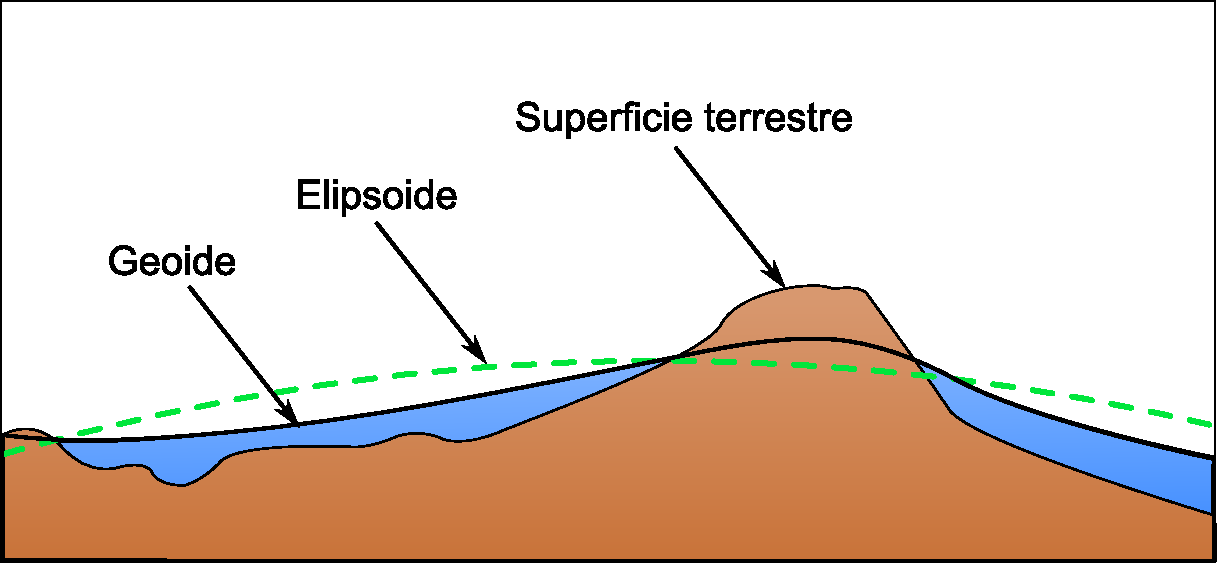
\includegraphics[width=.6\columnwidth]{Fundamentos_cartograficos/Tres_superficies.pdf}
\caption{\small Tres superficies fundamentales: superficie real de la Tierra, geoide y elipsoide (Adaptado de Wikipedia).}
\label{Fig:Tres_superficies} 
\end{figure}

En un elipsoide general, tanto la posici�n de su centro de gravedad como de su plano ecuatorial coinciden con los terrestres. Por el contrario, cuando el elipsoide es local, estas propiedades no han de cumplirse necesariamente, y el elipsoide a solas resulta insuficiente ya que carecemos de informaci�n sobre su posicionamiento con respecto a la superficie terrestre. 

Surge as� el concepto de \textbf{datum}, que es el conjunto formado por una superficie de referencia (el elipsoide) y un punto en el que <<enlazar>> este al geoide. Este punto se denomina \textbf{punto fundamental}, y en �l el elipsoide es tangente al geoide. La vertical al geoide y al elipsoide son id�nticas en el punto fundamental. 

Para un mismo elipsoide pueden utilizarse distintos puntos fundamentales, que dar�n lugar a distintos datum y a distintas coordenadas para un mismo punto.

\subsection{Sistemas de coordenadas}

Una vez hemos definido un modelo para definir la forma de la Tierra, podemos establecer un sistema de codificar cada una de las posiciones sobre su superficie y asignar a estas las correspondientes coordenadas. Para ello, encontramos dos opciones: utilizar los elementos de la \textbf{geometr�a esf�rica} y con estos definir el sistema de referencia, o utilizar la \emph{geometr�a plana}, para lo cual ser� necesario un mecanismo de \textbf{proyecci�n} de coordenadas que permita situar los elementos de la superficie del elipsoide sobre una superficie plana.

El sistema de \emph{coordenadas geogr�ficas} es un sistema de coordenadas esf�ricas mediante el cual un punto se localiza con dos valores angulares: \textbf{latitud}
y \textbf{longitud}. Las lineas de igual latitud o longitud se denominan \textbf{paralelos} y \textbf{meridianos} respectivamente.

Las coordenadas geogr�ficas resultan de gran utilidad, especialmente cuando se trabaja con grandes regiones. No obstante, no se trata de un sistema cartesiano, y tareas como la medici�n de �reas o distancias es mucho m�s complicada. Para poder crear cartograf�a y simplificar gran n�mero de operaciones posteriores, necesitamos coordenadas cartesianas. El proceso de asignar una coordenada plana a cada punto de la superficie de la Tierra (que no es plana) se conoce como \textbf{proyecci�n cartogr�fica}.

La superficie de la esfera no es \textbf{desarrollable}, es decir, no puede convertirse en un plano. Por ello, es necesario disponer de una metodolog�a para pasar puntos desde la superficie curva al plano, tal y como el que se muestra en la figura \ref{Fig:Proyeccion}.

\begin{figure}
\centering
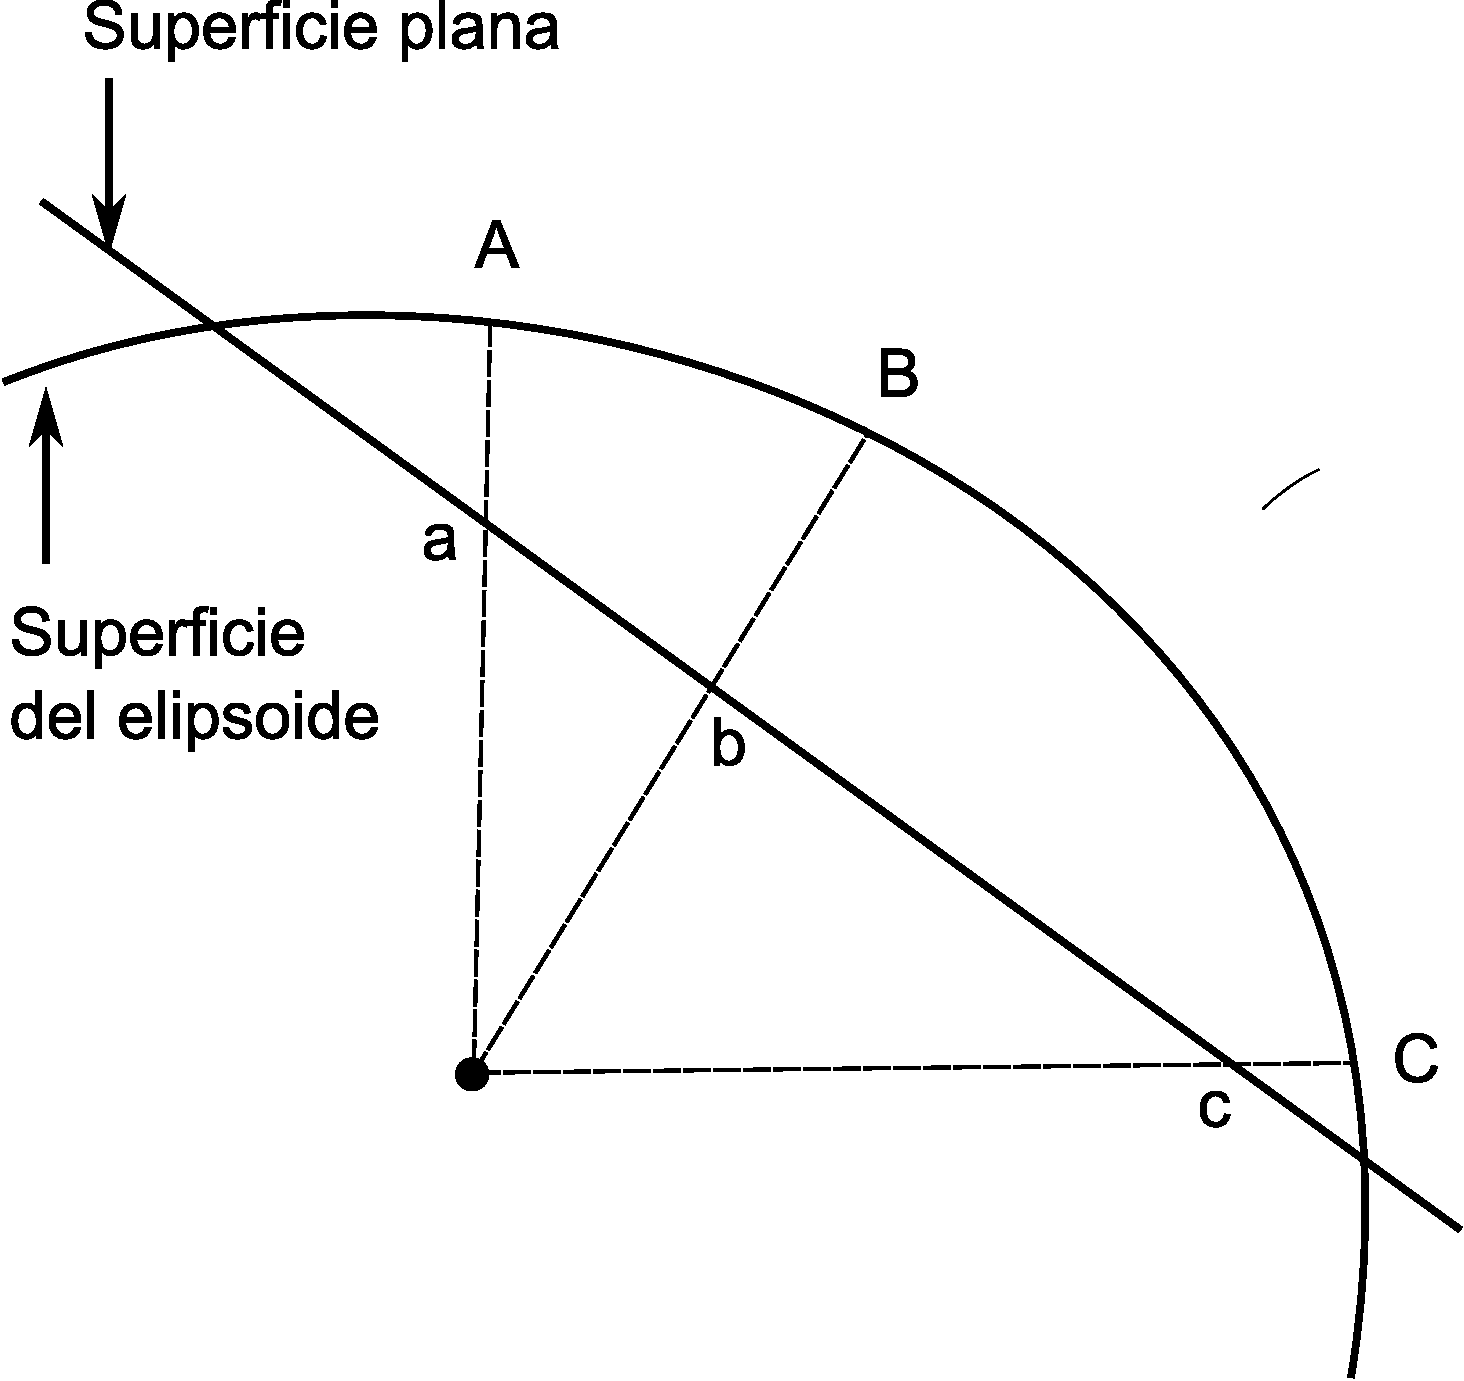
\includegraphics[width=.5\columnwidth]{Fundamentos_cartograficos/Proyeccion.pdf}
\caption{\small Esquema del concepto de proyecci�n. A los puntos $A, B$ y $C$ sobre la superficie del elipsoide se les asocian equivalentes $a, b$ y $c$ sobre un plano.}
\label{Fig:Proyeccion} 
\end{figure}


En el caso de la figura, los puntos se proyectan directamente sobre un plano. Otra opci�n es proyectarlos sobre una superficie tridimensional que, al contrario que la esfera, sea desarrollable. Las m�s habituales son el cilindro y el cono, que dan lugar a las \textbf{proyecciones c�nicas} y \textbf{cil�ndricas}.

Puede apreciarse en la figura que se producen distorsiones al realizar la proyecci�n. Por ejemplo, la distancia entre los puntos $A$ y $B$ no es igual a la existente entre los puntos $a$ y $b$. Con independencia de las caracter�sticas propias de la proyecci�n, siempre existen distorsiones, por ser la de la esfera una superficie no desarrollable. Estas distorsiones se conocen como \textbf{anamorfosis} . 


Seg�n las propiedades m�tricas que se conserven, las proyecciones pueden ser \textbf{equi�rea} (mantienen una escala constante), \textbf{conformes} (mantienen los �ngulos y la forma de los objetos) o \textbf{equidistantes} (mantienen las distancias).

La elecci�n de una u otra proyecci�n es funci�n de las necesidades concretas de cada caso de uso. 

En la actualidad, una de las proyecciones m�s extendidas en todos los �mbitos es la \textbf{proyecci�n universal transversa de Mercator}, la cual da lugar al \textbf{sistema de coordenadas UTM}. Este sistema no es simplemente una proyecci�n, sino un sistema completo para cartografiar la practica totalidad de la Tierra. Para ello, esta se divide en una serie de zonas rectangulares mediante una cuadricula y se aplica una proyecci�n y unos par�metros geod�sicos concretos a cada una de dichas zonas. En su forma actual, emplea un �nico elipsoide (WGS--84).

Con el sistema UTM, las coordenadas de un punto no se expresan como coordenadas terrestres absolutas, sino mediante la zona correspondiente y las coordenadas relativas a la zona UTM en la que nos encontremos.

La cuadricula UTM tiene un total de 60 husos numerados entre 1 y 60, cada uno de los cuales abarca una amplitud de 6\degree de longitud. El huso 1 se sit�a entre los 180\degree y 174\degree O, y la numeraci�n avanza hacia el Este. 

En latitud, cada huso se divide en 20 zonas, que van desde los 80\degree S hasta los 84\degree N. Estas se codifican con letras desde la C a la X, no utiliz�ndose las letras I y O por su similitud con los d�gitos 1 y 0. Cada zona abarca 8 grados de longitud, excepto la X que se prolonga unos 4 grados adicionales. 

Una zona UTM se localiza, por tanto, \textbf{con un n�mero y una letra}, y es en funci�n de la zona como posteriormente se dan las coordenadas que localizan un punto. Estas coordenadas se expresan en metros y expresan la distancia entre el punto y el origen de la zona UTM en concreto. El origen de la zona se sit�a en el punto de corte entre el meridiano central de la zona y el ecuador. 

Para evitar la aparici�n de n�meros negativos, se considera que el origen no tiene una coordenada X de 0 metros, sino de 500000, y una coordenada Y de 10000000 metros, lo cual hace que todas las coordenadas referidas a �l sean positivas.

\subsection{Transformaci�n y conversi�n de coordenadas}

Una situaci�n muy habitual en el trabajo con un SIG es disponer de cartograf�a en \textbf{varios sistemas de coordenadas}, o bien en un mismo sistema pero con par�metros diferentes (por ejemplo, diferente datum). Para poder emplear toda esa cartograf�a de forma conjunta, resulta necesario trabajar en un sistema �nico y bien definido, lo cual hace necesario convertir al menos una parte de ella. Cuando el datum es distinto en los sistemas de origen y destino, la \textbf{conversi�n de coordenadas} se conoce como \textbf{transformaci�n de coordenadas}.

Las operaciones de transformaci�n y conversi�n aparecen en los SIG como funcionalidades que permiten modificar los datos geogr�ficos, reemplazando sus coordenadas por coordenadas en otro sistema de coordenadas. Igualmente, aparecen como funcionalidades de representaci�n, permitiendo la conversi�n <<\textbf{al vuelo}>>, es decir, en tiempo real. En este caso, un dato en un sistema de coordenadas se puede representar en cualquier otro sin necesidad de una conversi�n previa, con lo que puede usarse conjuntamente con datos en un sistema de coordenadas distinto.

Para facilitar el uso de sistemas de referencia, existen proyectos de codificaci�n de estos, de forma que cada sistema existente puede identificarse de forma sencilla mediante un c�digo. El m�s extendido de estos es el sistema de codificaci�n \textbf{EPSG}.

\section{Conceptos cartogr�ficos b�sicos}
\label{Escala}

De entre los conceptos fundamentales de la cartograf�a que todo usuario de SIG ha de conocer, destaca el de \textbf{escala}. La escala  es la \textbf{relaci�n de tama�o} existente entre el mapa que se obtiene al desarrollar nuestra superficie de proyecci�n (de tama�o acorde con el objeto proyectado, esto es la Tierra) y el que finalmente manejamos, de tama�o m�s reducido. Conociendo esta relaci�n podemos conocer las verdaderas magnitudes de los elementos que vemos en el mapa, ya que podemos convertir las medidas hechas sobre el mapa en medidas reales. Es importante recordar que esas medidas no son tan <<reales>>, puesto que la propia proyecci�n las ha distorsionado ---lo cual no debe olvidarse---, pero s� que son medidas en la escala original del objeto cartografiado.

La escala se expresa habitualmente como un denominador que relaciona una distancia medida en un mapa y la distancia que esta medida representa en la realidad. Por ejemplo, una escala 1:50000 quiere decir que 1 cent�metro en un mapa equivale a 50000 cent�metros en la realidad, es decir a 500 metros. Este valor se conoce como \textbf{escala num�rica}.

Independientemente del tipo de proyecci�n, la escala es completamente cierta �nicamente en determinadas partes del mapa. En otros puntos de este, la escala var�a. La relaci�n entre la escala en esos puntos y la escala num�rica se conoce como \textbf{factor de escala}. 

Aunque tradicionalmente se entiende la escala como un concepto asociado a la representaci�n, los datos geogr�ficos tienen una escala inherente que no es funci�n de dicha representaci�n, sino del detalle con que han sido tomados. En este sentido es m�s conveniente entender la escala como un elemento relacionado con la \textbf{resoluci�n} de los datos, es decir, con el \textbf{tama�o m�nimo cartografiado}. Esta concepci�n no es en absoluto propia de los SIG, ya que deriva de las representaciones cl�sicas y los mapas impresos. Se sabe que el tama�o m�nimo que el ojo humano es capaz de diferenciar es del orden de 0,2 mm. Aplicando a este valor la escala a la que queremos crear un mapa, tendremos la m�nima distancia sobre el terreno que debe medirse. 

Es importante ser consciente de la limitaci�n que la escala considerada a la hora de la toma de datos (conocida como \textbf{escala operacional}) impone, especialmente en el contexto de un SIG. En un SIG, podemos aumentar el tama�o en pantalla de una cierta informaci�n geogr�fica, variando la escala de representaci�n (tambi�n conocida como \textbf{escala cartogr�fica}), pero ello no modifica la escala operacional. Por mucho que ampliemos no vamos a ver m�s detalles, ya que para ello ser�a necesario tomar m�s datos. 

Un tipo de datos particulares con los que se trabaja en un SIG, los datos \emph{r�ster}, tienen a su vez un par�metro de resoluci�n (el \textbf{tama�o de celda}) ligado a la escala. Veremos m�s al respecto en el cap�tulo \ref{Tipos_datos}.

\label{GeneralizacionCartografica}

Relacionado con el concepto de escala encontramos la denominada \textbf{generalizaci�n cartogr�fica}. Generalizar implicar expresar alguna idea o informaci�n de forma m�s resumida, de tal modo que esta sea comprensible y pueda aprovecharse de la mejor manera posible. La generalizaci�n es necesaria en un SIG para representar datos a una escala menor que su escala operacional, ya que a las limitaciones de la visi�n humana han de sumarse las limitaciones de resoluci�n que los dispositivos presentan. Por ejemplo, no tiene sentido representar el callejero de una ciudad a una escala peque�a como la que se utilizar�a para representar un mapa mundial, ya que cada peque�o punto de la pantalla contendr�a un gran n�mero de calles. Adem�s de obtener un resultado inservible, se consumir�an recursos en efectuar todos los c�lculos necesarios para producir esa representaci�n.

En ocasiones, el proceso de generalizaci�n es necesario por razones distintas a las anteriores, y requiere operaciones tambi�n distintas. Por ejemplo, podemos crear un mapa del mundo que contenga v�as de comunicaci�n, pero no todas, sino solo las principales autopistas de cada pa�s. En este caso, no vamos a encontrar problemas con distintas carreteras que se solapan en la representaci�n, ni tampoco un volumen excesivo de datos, pero debemos igualmente <<adaptar>> la representaci�n a la escala, es decir, efectuar alg�n tipo de generalizaci�n. En este caso, se representar�an las carreteras con un ancho mayor del real, ya que, de otro modo, no ser�an apenas visibles.

\begin{figure}
\centering
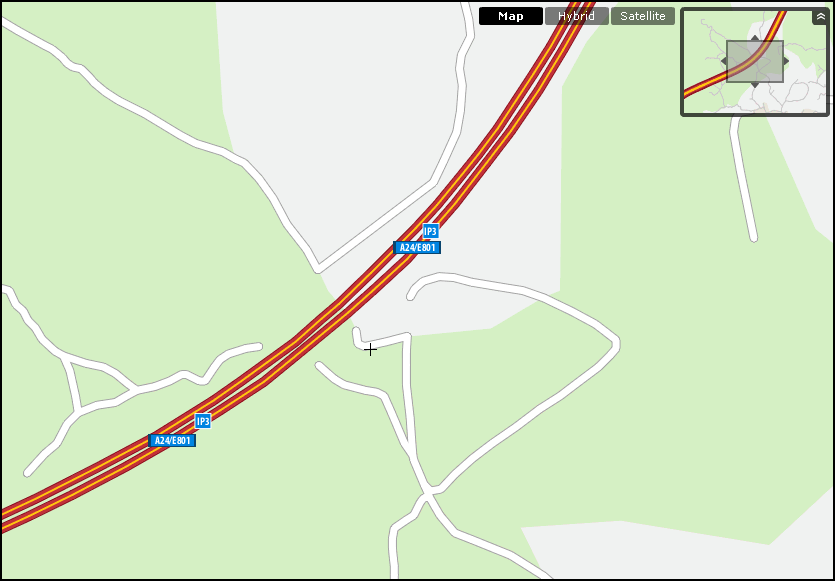
\includegraphics[width=.75\columnwidth]{Fundamentos_cartograficos/Generalizacion_agregacion.png}
\caption{\small Un ejemplo de generalizaci�n por agregaci�n. Dos carreteras pr�cticamente paralelas y unidas se representan como dos elementos en el mapa, pero en el localizador de la parte superior izquierda, a escala de menor detalle, se generalizan como una �nica (Tomado de Yahoo Maps).}
\label{Fig:Generalizacion_agregacion} 
\end{figure}

La generalizaci�n, por tanto, es un proceso que tiene como objetivo la producci�n de una imagen cartogr�fica \textbf{legible y expresiva}, reduciendo el contenido del mapa a aquello que sea posible y necesario representar. Para ello, se enfatiza lo que resulta de importancia y se suprime lo que carece de ella. 

Existen diversas operaciones que se emplean en el proceso de generalizaci�n. Algunas de las m�s relevantes son las \textbf{simplificaci�n} (representar un elemento menos complejo), la \textbf{agregaci�n} (representar varios elementos como uno solo ---Figura \ref{Fig:Generalizacion_agregacion}---), la \textbf{exageraci�n} (representar elementos con mayor tama�o del que les corresponde) y el \textbf{desplazamiento} (representar en una posici�n modificada, para garantizar la legibilidad). 




\label{Generalizacion_en_SIG}

En un SIG, la generalizaci�n puede incorporarse como parte de los propios mecanismos de representaci�n, aplic�ndose las transformaci�n correspondientes en tiempo real. A partir de un juego de datos, se elaboran las representaciones seg�n la escala a la que se est�n representando. Esta soluci�n tiene el inconveniente de producir resultados que no resultan �ptimos, por ser la generalizaci�n un proceso complejo y dif�cil de automatizar, y, sobre todo, el de consumir gran cantidad de recursos. La generalizaci�n en este caso tiene un objetivo cartogr�fico, pero en lugar de  hacer m�s fluido el trabajo con datos de gran volumen, lo hace m�s lento.

Una soluci�n alternativa y m�s adecuada de incorporar la generalizaci�n dentro de un SIG suele basarse en un enfoque multi--escalar (Figura \ref{Fig:SIG_multi_escala}), en el cual se maneja informaci�n de una misma zona de estudio a diferentes escalas, y se usa en cada momento aquella que resulte m�s conveniente. Si se trabajara con cartograf�a en papel, ser�a equivalente a tener varios mapas de una zona a diferentes escalas.

\begin{figure}
\centering
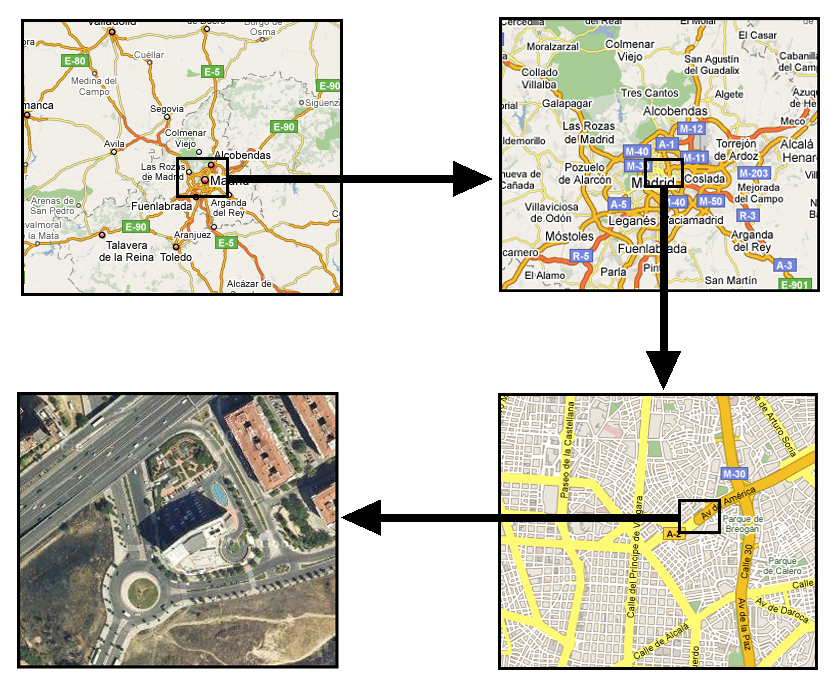
\includegraphics[width=\textwidth]{Fundamentos_cartograficos/SIG_multi_escala.png}
\caption{\small En un SIG es habitual manejar informaci�n a diferentes escalas. En funci�n de la escala de representaci�n, la informaci�n visualizada ser� una u otra.}
\label{Fig:SIG_multi_escala} 
\end{figure}


El concepto de \emph{capa},\index{Capa} que veremos en el cap�tulo \ref{Introduccion_datos} y que es vital para la idea actual de un SIG, permite este manejo simult�neo de informaci�n a distintas escalas.

En el caso de im�genes, este enfoque multi--escalar implica la creaci�n de las denominadas \textbf{pir�mides} (Figura \ref{Fig:Piramides}).


\begin{figure}
\centering
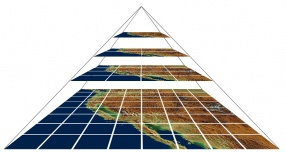
\includegraphics[width=.55\textwidth]{Fundamentos_cartograficos/Piramide.png}
\caption{\small Pir�mides de representaci�n con im�genes preparadas a distintas escalas (Fuente: OSGeo).}
\label{Fig:Piramides} 
\end{figure}

\pagestyle{empty}

\chapter{El dato geogr�fico y su almacenamiento}
\label{Introduccion_datos}



De todos los subsistemas de un SIG, el correspondiente a los datos es el pilar fundamental que pone en marcha los restantes. Los datos son el combustible que alimenta el SIG. El subsistema de datos es, a su vez, el m�s interrelacionado, y est� conectado de forma inseparable a todos los restantes. 


\pagestyle{fancy}

\section{Datos \emph{vs} Informaci�n. Tipos de informaci�n.}

Existe una importante diferencia entre los conceptos de \textbf{datos} e \textbf{informaci�n}. Un SIG es un Sistema de \emph{Informaci�n} Geogr�fica, pero maneja \emph{datos} geogr�ficos, existiendo diferencias entre estos conceptos.

Entendemos como dato al simple conjunto de valores o elementos que utilizamos para representar algo. Por ejemplo, el c�digo 502132N es un dato. 

El dato anterior podemos interpretarlo como si fuera una referencia geogr�fica, y cuyo significado ser�a entonces una latitud, en particular 50\degree $21'$ $32''$ Norte. Si lo interpretamos como un c�digo que hace referencia a un documento de identificaci�n de una persona, la informaci�n que nos aporta es en ese caso completamente distinta. El dato ser�a el mismo, formado por seis d�gitos y una letra, pero la informaci�n que da es diferente, ya que lo entendemos e interpretamos de manera distinta.

La informaci�n es, por tanto, el resultado de un dato y una \textbf{interpretaci�n}, y el trabajo con datos es en muchos casos un proceso enfocado a obtener de estos toda la informaci�n posible. 

Comprender el significado y las diferencias entre datos e informaci�n permiten entender entre otras cosas que la relaci�n entre los vol�menes de ambos no es necesariamente constante. Por ejemplo, los datos 502132NORTE o CINCUENTA VEINTIUNO TREINTAYDOS NORTE son mayores en volumen que 502132N, pero recogen la misma informaci�n espacial que este (suponiendo que los interpretamos como datos de latitud). 

En la informaci�n geogr�fica se distinguen dos componentes: \textbf{espacial} y \textbf{tem�tica}. La componente espacial hace referencia a la posici�n dentro de un sistema de referencia establecido, y responde a la pregunta \emph{�d�nde?}. La componente tem�tica responde a la pregunta \emph{�qu�?}, y define la naturaleza del fen�meno que se produce en la localizaci�n indicada por la componente espacial.


Mientras que la componente espacial va a ser generalmente un valor num�rico, pues son de esa naturaleza los sistemas de coordenadas que permiten expresar una posici�n concreta en referencia a un marco dado, la componente tem�tica puede ser \textbf{num�rica} o \textbf{alfanum�rica} (texto). Una variable num�rica puede a su vez ser de cuatro tipos: \textbf{nominal, ordinal, intervalo} o \textbf{raz�n}.


El tipo de variable condiciona las operaciones que pueden realizarse con un dato geogr�fico en funci�n de c�mo sea su componente tem�tica. 

Un concepto a tener en cuenta en relaci�n con las componentes de la informaci�n geogr�fica es la \textbf{{dimensi�n}}. Los elementos que registramos pueden ir desde sencillos puntos (0D) hasta vol�menes tridimensionales (3D).

Las diferentes formas de representar y almacenar la informaci�n, que veremos m�s adelante en este capitulo, dependen del tipo de variable con que se trabaje.



\section{Divisi�n de la informaci�n. Capas}

En un SIG, la informaci�n espacial referida a una zona de estudio est� dividida en varios niveles, de tal forma que, pese a coincidir sobre un mismo emplazamiento, informaci�n sobre distintas variables se encuentra recogida de forma independiente. Es decir, en funci�n de la componente tem�tica se establecen distintos bloques de datos espaciales. Cada uno de estos bloques tem�ticos se conoce como \textbf{capa} (Figura \ref{Fig:Concepto_capa}). 

\begin{figure}[!hbt] 
\centering
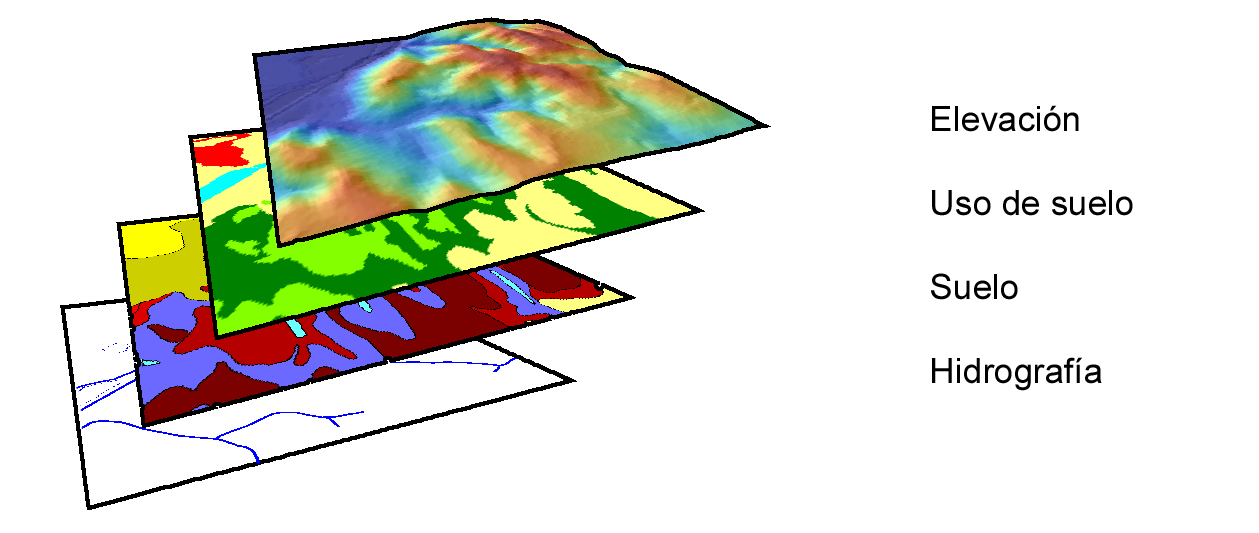
\includegraphics[width=.7\textwidth]{Introduccion_datos/Concepto_capa.png}
\caption{\small Concepto de \emph{capa} de informaci�n geogr�fica dentro de un SIG}
\label{Fig:Concepto_capa} 
\end{figure}

El concepto de capa es imprescindible para comprender todo SIG, y  favorece la correcta estructuraci�n de la informaci�n y el trabajo con ella. Toda la informaci�n geogr�fica con que trabajemos en un SIG va a ser en forma de capas. Cada una de ellas puede abrirse de forma independiente en un SIG y utilizarse por s� misma o en conjunto con otras.

Con la cartograf�a cl�sica, no es posible (o resulta dif�cil e impreciso) combinar distintos tipos de informaci�n, como por ejemplo la contenida en un mapa topogr�fico y la existente en un mapa de tipos de suelo y otro de vegetaci�n potencial. En el caso de un SIG, los distintos tipos de informaci�n se pueden combinar de forma sencilla y limpia, y no aparecen los mismos problemas

La relevancia del concepto de capa como elemento fundamental de un SIG es enorme, pues constituye el marco b�sico sobre el que se van a llevar a cabo gran parte de las operaciones. Por ejemplo, vimos en el apartado dedicado a la generalizaci�n cartogr�fica c�mo en un SIG podemos utilizar diferentes <<versiones>> de los datos correspondientes a una zona concreta, y representar una u otra de ellas en funci�n de la escala de trabajo. Estas versiones se almacenar�n como distintas capas. La capa es as� la unidad fundamental no solo en t�rminos de un �rea dada, sino tambi�n de una escala concreta, y permite una divisi�n de los datos �ptima a todos los efectos.


La separaci�n de la informaci�n en capas evita asimismo la redundancia de datos, ya que cada capa contiene un tipo de informaci�n concreto. En un mapa cl�sico se presentan siempre varias variables, algunas de ellas presentes con car�cter general, tales como nombres de ciudades principales o v�as m�s importantes de comunicaci�n. En un SIG, al encontrarse estas variables separadas en sus correspondientes capas, es el usuario quien las combina.

El trabajo con capas permite, por tanto, una estructura \textbf{m�s organizada} y una \textbf{mayor atomizaci�n} de los datos, con las consecuentes ventajas en el almacenamiento, manejo y funcionalidad que esto conlleva.


Adem�s de dividir la informaci�n geogr�fica en capas de acuerdo con su contenido, tambi�n dividimos esta con criterios puramente espaciales, <<cort�ndola>> en unidades menores que ocupen una regi�n de amplitud m�s reducida. Este es un procedimiento similar al que encontramos en un mapa impreso, ya que el territorio de un pa�s se encuentra cartografiado en diferentes \emph{hojas}. 

La principal cualidad de un SIG para integrar de forma transparente datos correspondientes a zonas distintas y formar un mosaico �nico es la \textbf{separaci�n que existe entre datos y visualizaci�n}. Los datos son la base de la visualizaci�n, pero en un SIG estos elementos conforman partes del sistema bien diferenciadas. Esto quiere decir que los datos se emplean para crear un resultado visual pero en s� mismos no contienen valores relativos a esa visualizaci�n.

De este modo, es posible combinar los datos y despu�s representarlos en su conjunto. Un proceso as� no puede realizarse con un mapa ya impreso, pues este contiene ya elementos de visualizaci�n e incluso componentes cartogr�ficos tales como una flecha indicando el Norte, una leyenda o una escala. Por ello, aunque puedan combinarse, realmente no se <<funde>> la informaci�n de cada uno de los mapas para conformar uno �nico. En un SIG, por el contrario, la visualizaci�n de cuatro o m�s bloques de datos puede ser id�ntica a la que obtendr�a si todos esos datos constituyeran un �nico bloque. 

\section{Modelos para almacenamiento de informaci�n geogr�fica}
\label{Tipos_datos}

El proceso de convertir un �rea geogr�fica y la informaci�n acerca de ella en un dato susceptible de ser incorporado a un SIG puede dividirse en tres fases:

\begin{itemize}
 \item Establecimiento de un \textbf{modelo geogr�fico}. Es decir, un modelo conceptual de la realidad geogr�fica y su comportamiento.
\item Establecimiento de un \textbf{modelo de representaci�n}. Es decir, una forma de recoger el anterior modelo conceptual y sus caracter�sticas propias, reduci�ndolo a una serie finita de elementos.
\item Establecimiento de un \textbf{modelo de almacenamiento}. Es decir, un esquema de c�mo almacenar los distintos elementos del modelo de representaci�n.
\end{itemize}
\index{Modelo!geogr�fico}\index{Modelo!de representacion}\index{Modelo!de almacenamiento}



Por su mayor importancia, nos centraremos en los modelos de representaci�n. Los modelos de representaci�n que se utilizan principalmente en un SIG son dos: \textbf{modelo raster} y \textbf{modelo vectorial}. Las capas que utilizan estos modelos se conocen como \textbf{capas raster} y \textbf{capas vectoriales}, y esta es la terminolog�a habitual en el �mbito de los SIG para referirse a la naturaleza de una determinada capa. 

\subsection{Modelo r�ster}

El modelo r�ster se basa en una \textbf{divisi�n sistem�tica} del espacio. Todo el espacio queda cubierto y caracterizado como un conjunto de unidades elementales, cada una de ellas con un valor asociado.  

Lo m�s habitual es una divisi�n en una malla de \textbf{celdas cuadradas} o rectangulares. Conociendo la orientaci�n de la malla y las dimensiones de cada una de las celdas, as� como las coordenadas de al menos una de ellas, es posible conocer las coordenadas del resto en virtud de su \textbf{estructura regular}. Con esto, conocemos los valores de la variable en todos los puntos del espacio cubierto por la capa. El \textbf{tama�o de celda} es un par�metro relacionado con la escala de trabajo de la capa, ya que define la resoluci�n de esta y est� en funci�n de la precisi�n con que se han tomado los datos correspondientes.


La figura \ref{Fig:Raster_closeup} muestra un ejemplo de una malla r�ster con valores de elevaci�n.

\begin{figure}[!hbt]   
\centering
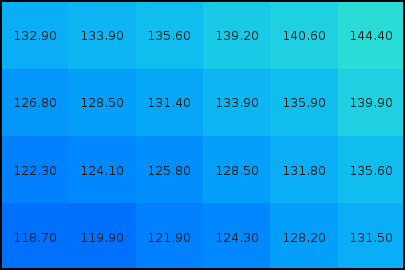
\includegraphics[width=.6\textwidth]{Tipos_datos/Raster_closeup.png}
\caption{\small Celdas de una malla r�ster con sus valores asociados.}
\label{Fig:Raster_closeup} 
\end{figure}

El n�mero de valores distintos recogidos para cada celda coincide con el n�mero de las denominadas \textbf{bandas}. Una banda contiene un �nico valor en una capa raster. Puede entenderse una capa raster de m�s de una banda como un conjunto de capas (cada banda ser�a una subcapa de ese conjunto), teniendo en todas ellas la malla de celdas las mismas caracter�sticas espaciales, y presentandose el conjunto como un �nico elemento. 

El ejemplo m�s claro de uso del modelo raster lo encontramos en las im�genes. Una imagen digital se compone de una malla de elementos (denominados \textbf{p�xeles}, cada uno de los cuales tiene un color asociado). El conjunto de estos p�xeles forman la imagen completa. Lo m�s habitual es que las im�genes contengan 3 bandas, correspondientes a las intensidades de los colores rojo, verde y azul, las cuales al combinarse permiten obtener el color de cada p�xel.

Otro uso habitual del modelo raster es en los denominados \textbf{Modelos Digitales de Elevaciones} (MDE), que recogen la topograf�a de un terreno. El modelo raster es el habitual de capa raster son las capas con modelos
De forma general, los valores de una capa r�ster, en cualquiera de sus bandas, son casi exclusivamente num�ricos, no estando los SIG preparados para manejar otro tipo de valores en la componente tem�tica de una capa r�ster. De esta forma, una capa raster puede equipararse al concepto matem�tico de una \textbf{matriz}, con las ventajas que ello supone para aplicar sobre ella herramientas matem�ticas a la hora de su an�lisis.




\subsection{Modelo vectorial}


El otro modelo principal de representaci�n es el modelo vectorial. En este modelo, no existen unidades fundamentales que dividen la zona recogida, sino que se recoge la variabilidad y caracter�sticas de esta mediante \textbf{entidades}, para cada una de las cuales dichas caracter�sticas son constantes. Las entidades se componen de \textbf{primitivas geom�tricas}, y estas pueden ser de tres tipos: \textbf{puntos, l�neas} y \textbf{pol�gonos}.

\begin{figure}[!hbt]   
\centering
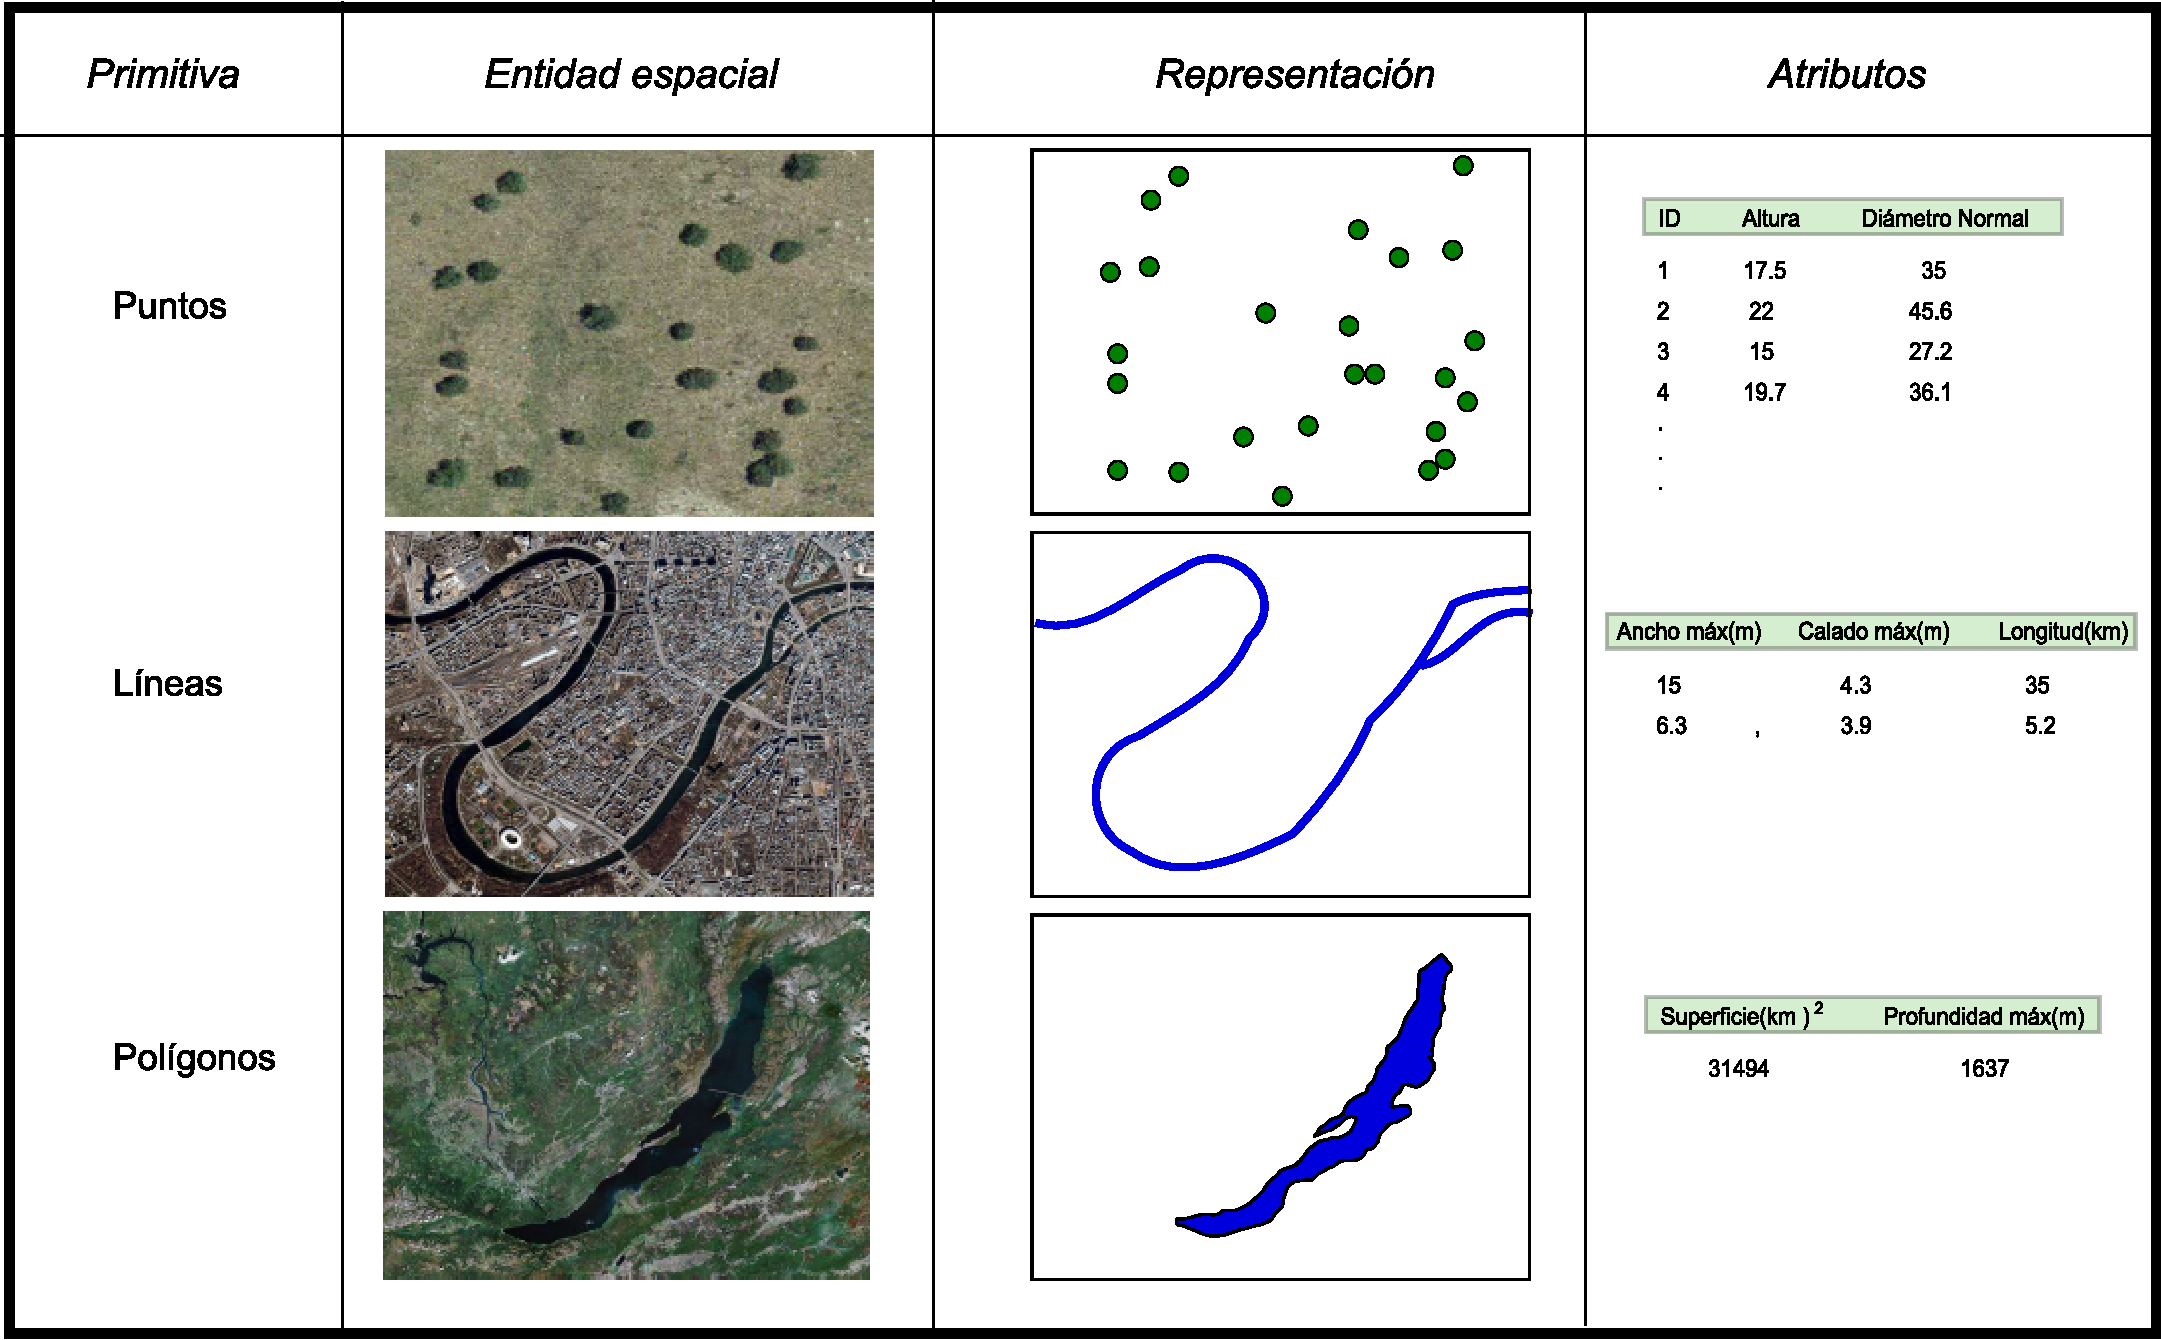
\includegraphics[width=\textwidth]{Tipos_datos/Primitivas_vectoriales.pdf}
\caption{\small Primitivas geom�tricas en el modelo de representaci�n vectorial y ejemplos particulares de cada una de ellas con atributos asociados}
\label{Fig:Primitivas_vectoriales} 
\end{figure}

Utilizando puntos, l�neas o pol�gonos, puede modelizarse el espacio geogr�fico si se asocia a estas geometr�as una serie de valores definitorios. Una entidad puede tener \textbf{varias primitivas}. Por ejemplo, en una capa de pa�ses, necesitar�amos varios conjuntos para representar Espa�a si queremos incluir tanto la peninsula como las islas que la forman. Todos estos pol�gonos constituyen una �nica entidad, ya que todos pertenecen al mismo pa�s y tendr�n el mismo conjunto de valores asociados.

A la hora de definir las formas geom�tricas b�sicas, todas ellas pueden en �ltima instancia \textbf{reducirse a puntos}. As�, las l�neas son un conjunto de puntos interconectados en un determinado orden, y los pol�gonos son l�neas cerradas, tambi�n expresables por tanto como una serie de puntos. Todo elemento del espacio geogr�fico queda definido, pues, por una serie de puntos que determinan sus propiedades espaciales y una serie de valores asociados.

Dentro de un SIG, una capa vectorial puede contener \textbf{un �nico tipo de primitiva}. As�, tenemos capas vectoriales de puntos, de l�neas y de pol�gonos, respectivamente. Una variable puede recogerse con varios tipos de primitivas (por ejemplo, puede indicarse una ciudad con un punto o con un pol�gono que delimite su per�metro), y la elecci�n de uno u otro tipo de geometr�a ha de ser funci�n del tipo de fen�meno que se pretende modelizar o la precisi�n necesaria, entre otros factores. 

La componente tem�tica en el modelo vectorial se establece mediante los denominados \textbf{atributos}, que suelen ser m�ltiples, a diferencia de lo que sucede en el modelo raster, donde lo habitual es tener un �nico valor para cada celda. Los atributos de una capa vectorial pueden contener informaci�n de cualqueir clase, siendo m�s vers�tiles que en el caso de las capas r�ster, donde ya vimos que se maneja �nicamente informaci�n num�rica. Por su estructura particular (series de atributos asociados a una entidad), la componente tem�tica en el modelo vectorial se presta especialmente a representarse en tablas y almacenarse en una \textbf{base de datos}, y puede analizarse independientemente de la componente espacial. 

Un elemento particular del modelo de representaci�n vectorial es la \textbf{topolog�a}.  Una capa vectorial contiene topolog�a si en ella se almacenan de alg�n modo las relaciones espaciales que existen entre sus elementos. Disponer de topolog�a en una capa vectorial es de gran importancia a la hora de llevar a cabo ciertos tipos de an�lisis, as� como procedimientos tales como la edici�n de los propios datos geogr�ficos. 

Aunque la mayor�a de operaciones con una capa vectorial pueden llevarse a cabo en ausencia de topolog�a, algunas de ellas como el \textbf{an�lisis de redes} no se pueden llevar a cabo sin topolog�a. Si pensamos en una capa de v�as sobre la que desarrollar ese an�lisis de redes, un mero conjunto de elementos geom�tricos (l�neas en este caso), no nos da informaci�n sobre los posibles enlaces entre las v�as que quedan representadas. Los puntos donde se cruzan dos v�as pueden ser cruces o rotondas (es decir, puede pasarse de una v�a a otra, existiendo conexi�n entre ellas), o bien pasos elevados o subterr�neos donde una de las v�as pasa por encima de la otra (y por tanto no existe comunicaci�n entre ambas). Las circunstancias son muy distintas en funci�n del tipo de cruce que exista, y por ello es imprescindible conocer esta informaci�n para efectuar un an�lisis de redes correcto (Figura \ref{Fig:Topologia_vias})

\begin{figure}[!hbt]   
\centering
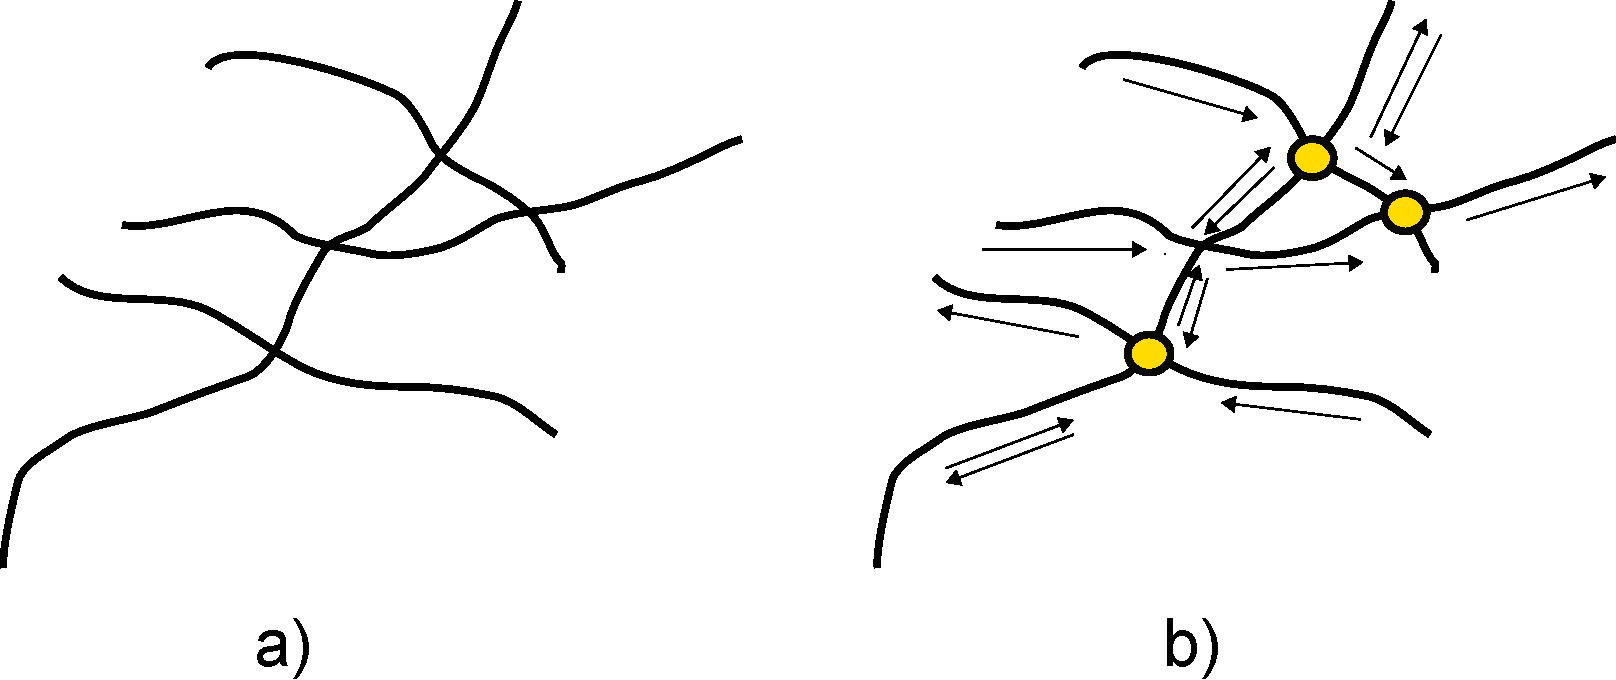
\includegraphics[width=.6\columnwidth]{Tipos_datos/Topologia_vias.pdf}
\caption{\small Capa de v�as de comunicaci�n sin topolog�a (a) o con ella (b). Los puntos en este segundo caso indican conexiones entre vias, y son una representaci�n visible de la topolog�a existente. }
\label{Fig:Topologia_vias} 
\end{figure}


El almacenamiento de entidades basado en una mera lista de coordenadas de cada entidad, sin topolog�a,  se conoce popularmente como \emph{spaghetti}, pues si pensamos en una capa de lineas sin topolog�a que se entrecruzan en el espacio, esta se asemejan en cierta forma a un ca�tico plato de \emph{spaguettis} sin orden ni relaci�n entre ellos.


\subsection{Raster \emph{vs} vectorial}


Tanto el modelo raster como el vectorial pueden emplearse para recoger \textbf{cualquier tipo de informaci�n}. La figura \ref{Fig:Esquemas_modelos_representacion} muestra un ejemplo de esto, representando una capa de v�as seg�n ambos modelos. Otro ejemplo para mostrar esto lo encontrarmos en las capas de elevaciones, que ya hemos visto que suelen recogerse en capas raster, en especial si se va a desarrollar sobre ellas alg�n tipo de an�lisis. No obstante, pueden recogerse tambi�n como una capa vectorial de puntos (este es una caso habitual si se obtienen los datos de un levantamiento topogr�fico), o bien como una capa de l�neas que contenga \textbf{curvas de nivel}, entre otras opciones.

\begin{figure}[!hbt]   
\centering
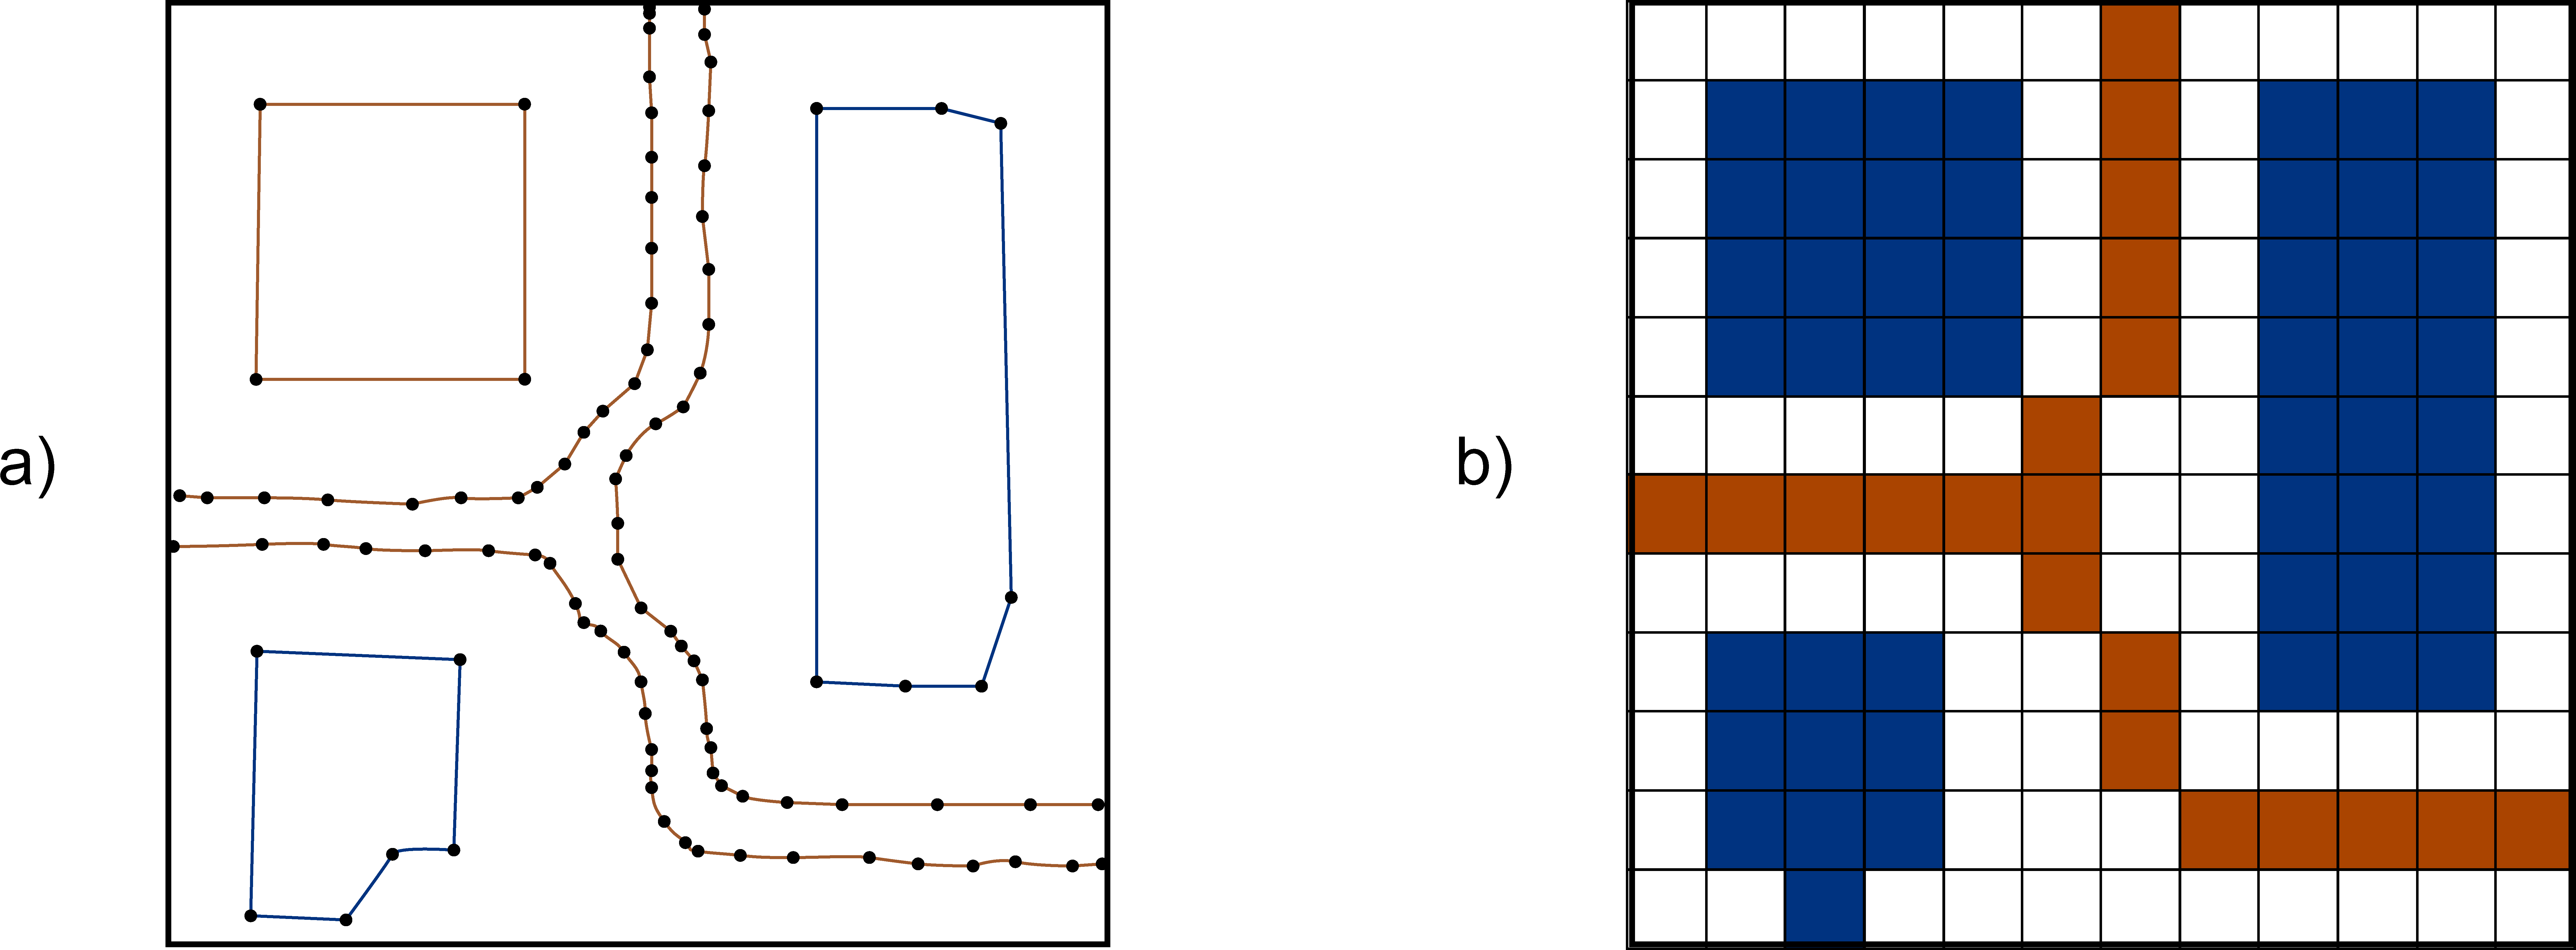
\includegraphics[width=.9\textwidth]{Tipos_datos/Esquemas_modelos_representacion.pdf}
\caption{\small Comparaci�n entre los esquemas del modelo de representaci�n vectorial (a) y r�ster (b).}
\label{Fig:Esquemas_modelos_representacion} 
\end{figure}


Resulta obvio que las diferencias entre los modelos r�ster y vectorial son muy notables, y que cada uno de ellos posee sus propias ventajas e inconvenientes. 
Algunos aspectos a los cuales puede atenderse para comparar uno y otro modelo son los siguientes:

\begin{itemize}
\item \textbf{Planteamiento}. El modelo r�ster hace m�s �nfasis en aquella caracter�stica del espacio que analizamos (\emph{qu�} y \emph{c�mo}), mientras que el modelo vectorial da prioridad a la localizaci�n de dicha caracter�stica (\emph{d�nde})
 \item \textbf{Precisi�n}. El modelo r�ster tiene su precisi�n limitada por el tama�o de celda. Las entidades menores que dicho tama�o de celda no pueden recogerse, y la variaci�n espacial que sucede dentro del espacio de la celda tampoco. 

Asimismo, existe una imprecisi�n en las formas. El detalle con el que puede recogerse la forma de una entidad geogr�fica seg�n el modelo vectorial es, en la pr�ctica, ilimitado, mientras que, como puede verse en la imagen \ref{Fig:Imprecision_raster}, el modelo r�ster restringe las formas a �ngulos rectos, ya que la unidad base es un cuadrado. 

\begin{figure}[!hbt]   
\centering
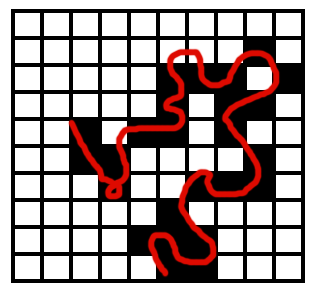
\includegraphics[width=.5\columnwidth]{Tipos_datos/Imprecision_raster.png}
\caption{\small Imprecisi�n de forma en el modelo de representaci�n r�ster. La divisi�n del espacio en unidades cuadradas impide la representaci�n fiel de entidades tales como curvas.}
\label{Fig:Imprecision_raster} 
\end{figure}

\item \textbf{Complejidad}. La regularidad y sistematicidad de las mallas r�ster hacen sencillo el implementar algoritmos de an�lisis, muy especialmente aquellos que implican el uso combinado de varias capas. Por el contrario, la irregularidad espacial de las capas vectoriales hace que la implementaci�n de los mismos algoritmos sea sumamente m�s compleja si se trabaja con estas capas.


\end{itemize}

No existe un modelo de representaci�n id�neo de forma global, sino que esta idoneidad depende de muchos factores, como por ejemplo:

\begin{itemize}
 \item \textbf{Tipo de variable o fen�meno a recoger}. Las variables \textbf{continuas} tales como la elevaci�n es m�s adecuado en general recogerlas en capas raster, para as� facilitar su an�lisis, mientras que las variables \textbf{discretas} es preferible almacenarlas como capas vectoriales.
\item \textbf{Tipo de an�lisis o tarea a realizar sobre dicha variable}. El uso que demos a una capa tem�tica condiciona en gran medida el modelo de datos id�neo. Por ejemplo, en el caso de una capa de elevaciones, su an�lisis se lleva mejor a cabo si esta informaci�n est� recogida seg�n el modelo r�ster. Sin embargo, si el objetivo principal es la visualizaci�n de esa elevaci�n en conjunto con otras variables, unas curvas de nivel pueden resultar m�s adecuadas, ya que, entre otras cosas, no interfieren tanto con otros elementos a la hora de dise�ar un mapa con todas esas variables.
\item \textbf{Contexto de trabajo}. Por ejemplo, si queremos trabajar con im�genes, esto nos condiciona al empleo de datos r�ster, ya que resulta mucho m�s sencillo combinarlos con las im�genes, las cuales siempre se presentan como capas r�ster. 
\end{itemize}


Existen procedimientos para \textbf{convertir} entre los formatos r�ster y vectorial, de forma que el disponer de datos en un modelo de representaci�n particular no implica que debamos desarrollar nuestro trabajo sobre dichos datos directamente, sino que podemos efectuar previamente una conversi�n. Los cap�tulos \ref{Creacion_capas_raster} y \ref{Creacion_capas_vectoriales} tratan estos temas en profundidad.




\pagestyle{empty}

\chapter{Fuentes principales de datos espaciales}
\label{Fuentes_datos}




No hace tanto tiempo, toda la informaci�n que se manejaba dentro de un SIG ten�a su origen en un mapa en papel, el cual deb�a \emph{prepararse} para adaptarse a la naturaleza propia del SIG. El dato geogr�fico se obten�a a partir de la \textbf{digitalizaci�n} de cartograf�a, es decir, convertir los datos geogr�ficos en formato impreso en datos en formato digital que un SIG pudiera manejar. 

Un SIG implica una aplicaci�n inform�tica, y esta se alimenta en �ltima instancia exclusivamente de datos digitales. Los datos geogr�ficos digitales tienen una serie de ventajas frente a los anal�gicos (adem�s del mero hecho de que podemos incorporarlos a nuestro SIG), y suponen, como sucede en muchos otros campos, un salto cualitativo importante. Entre estas ventajas, que son a su vez comunes a otros �mbitos,  destacan la sencillez de actualizaci�n, la facilidad de distribuci�n (en especial con la aparici�n de Internet), el menor espacio f�sico necesario para su almacenamiento, la facilidad y precisi�n del an�lisis, y la facilidad de mantenimiento (el dato digital no se degrada, lo que se degrada es su soporte, pero es sencillo replicar el dato sin p�rdida de calidad)

Hoy en d�a las t�cnicas de adquisici�n de datos han evolucionado y permiten crear datos que pueden ser directamente integrados en un SIG. Distinguimos as� \textbf{fuentes de datos primarias} y \textbf{secundarias}. 

Las fuentes de datos primarias son aquellas cuyos datos podemos emplear en un SIG, ya que estos, en su forma original, ya son susceptibles de ser sometidos a las operaciones de manejo y an�lisis que incorporan los SIG. Por su parte, las fuentes de datos secundarias generan datos que no pueden emplearse en un SIG sin un proceso de adaptaci�n previo, siendo el dato derivado el que utilizamos en un SIG, no el original. 

En este cap�tulo, veremos las distintas fuentes de datos con las que podemos trabajar un en SIG.


\section{Teledetecci�n}\index{Teledetecci�n}

La primera fuente de datos que trataremos en este cap�tulo es la teledetecci�n. Entendemos por teledetecci�n el estudio y medida de las caracter�sticas de una serie de objetos (en nuestro caso elementos de la superficie terrestre) sin que exista contacto f�sico. Para ello, se miden las perturbaciones que el objeto provoca en su entorno, principalmente las de tipo electromagn�tico.

Un sistema de teledetecci�n cuenta con los siguientes elementos (Figura \ref{Fig:Elementos_teledeteccion}):

\begin{figure}[!hbt]   
\centering
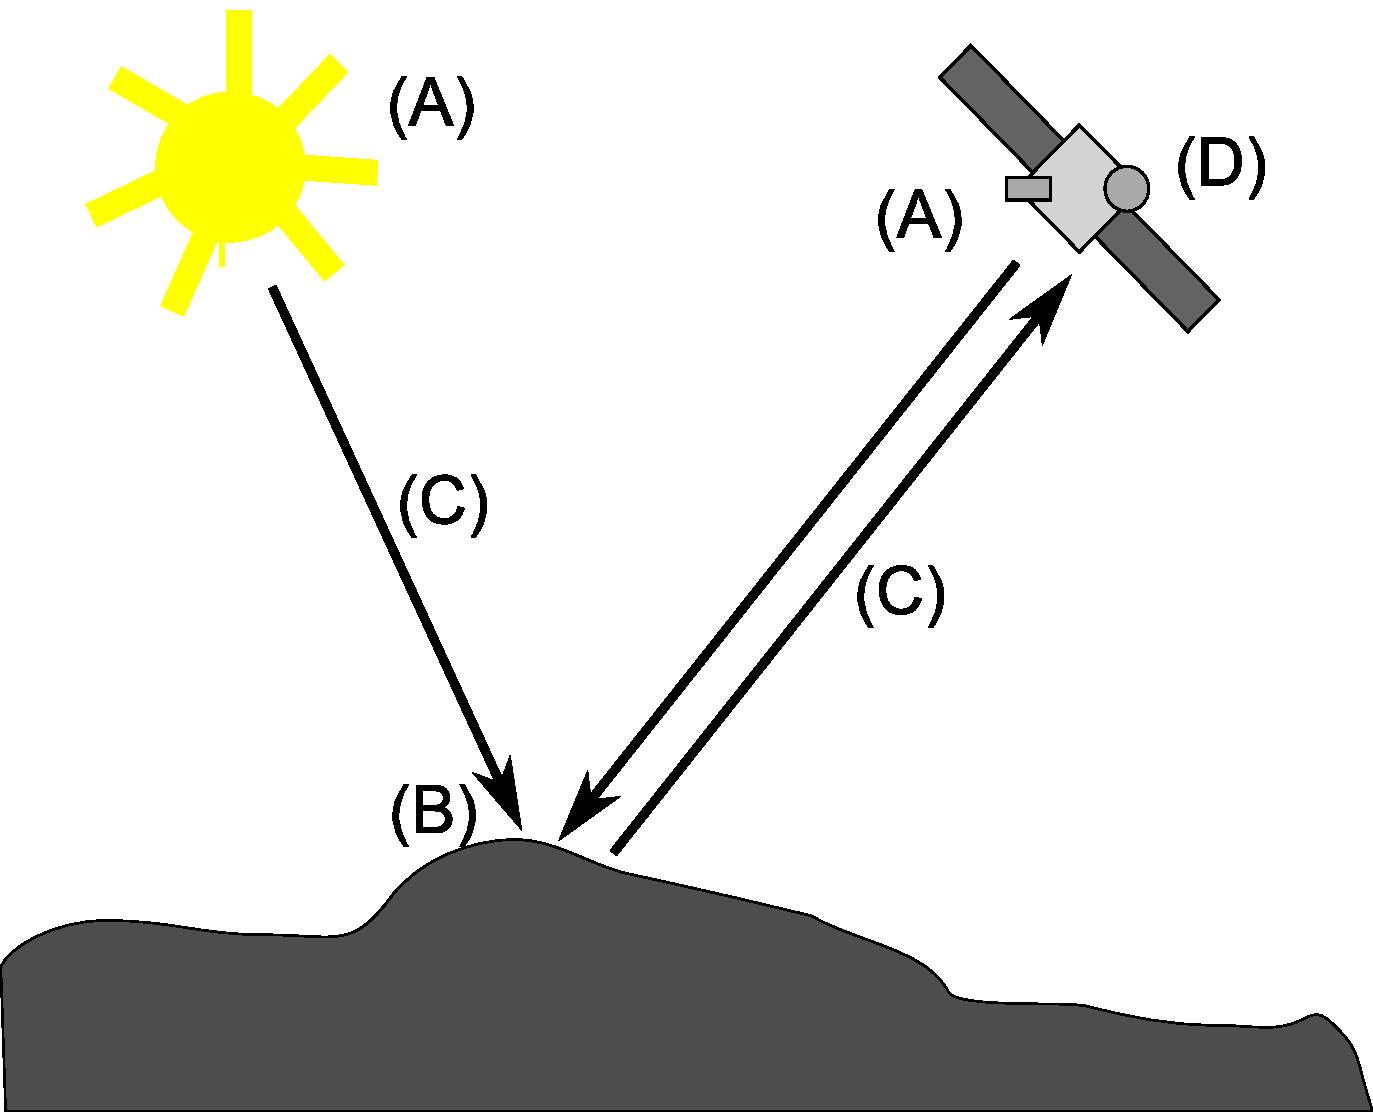
\includegraphics[width=.4\textwidth]{Fuentes_datos/Elementos_teledeteccion.pdf}
\caption{\small Esquema de un sistema de teledetecci�n.}
\label{Fig:Elementos_teledeteccion} 
\end{figure}


\begin{itemize}
	\item \textbf{Una fuente de radiaci�n (A)}\index{Fuente de radiaci�n}. Puede ser de origen natural o artificial. La radiaci�n emitida por dicha fuente llega al terreno y sufre una perturbaci�n causada por los elementos de este, siendo esta perturbaci�n el objeto de estudio de la teledetecci�n. Los propios objetos pueden ser tambi�n emisores ellos mismos de radiaci�n.
	\item \textbf{Unos objetos (B) que interaccionan con la radiaci�n} o la emiten, seg�n lo anterior.
	\item \textbf{Una atm�sfera (C)} por la que se desplaza la radiaci�n, tanto desde la fuente hasta el objeto como desde el objeto hasta el receptor. La atm�sfera tambi�n interact�a con la radiaci�n, introduciendo igualmente perturbaciones en ella.
	\item \textbf{Un receptor (D) que recoge la radiaci�n} una vez esta ha sido perturbada o emitida por los objetos. El receptor va a generar como producto final una imagen (en t�rminos de un SIG, una capa r�ster), en cuyas celdas o p�xeles se va a contener un valor que indica la intensidad de la radiaci�n. Estos valores son valores enteros que indican el nivel de dicha radiaci�n dentro de una escala definida (habitualmente valores entre 1 y 256), y se conocen dentro del �mbito de la teledetecci�n como \textbf{Niveles Digitales}.
\end{itemize}

A lo largo de este apartado veremos con detalle estos elementos. Para estudiar los dos primeros, estudiaremos los fundamentos f�sicos relativos a la radiaci�n y a la la interacci�n entre esta y la materia, mientras que para el estudio del sistema receptor analizaremos los elementos de este en dos componentes por separado: sensores y plataformas. 

La interacci�n de la atm�sfera interesa de cara a eliminar su efecto, ya que lo que resulta de inter�s en general son los objetos en la superficie terrestre, no la atm�sfera como tal. Eliminar esta influencia de la atm�sfera es parte de los procesos posteriores que se realizan con la imagen, y que se detallan en los cap�tulos dedicados al an�lisis de im�genes en lugar de en este.

\subsection{Fundamentos f�sicos}

La radiaci�n electromagn�tica es producto de las alteraciones en los campos el�ctrico y magn�tico, las cuales generan ondas correspondientes a cada uno de los campos magn�tico y el�ctrico. Estas ondas se desplazan a la velocidad de la luz, y se pueden describir con los par�metros habituales, tales como la longitud de onda o la frecuencia. El rango de longitudes de onda cubierta por la radiaci�n electromagn�tica se conoce como \textbf{espectro electromagn�tico}.

El espectro se subdivide en regiones en funci�n de su longitud de onda, tales como (de menor a mayor longitud de onda) los rayos $\gamma$, los rayos X, la regi�n ultravioleta, la regi�n visible, la regi�n infraroja, o las microondas  

La radiaci�n emitida por una fuente de radiaci�n es alterada por la presencia de los distintos objetos, ya que estos \textbf{absorben, transmiten} o \textbf{reflejan} esta.

Estos tres fen�menos se dan en diferente proporci�n en funci�n de las caracter�sticas del objeto y de la radiaci�n. La parte que  interesa a efectos de la teledetecci�n es aquella que se refleja en el objeto, ya que esta es la que posteriormente puede recogerse y emplearse para la generaci�n de las im�genes.

Como ya se dijo en el cap�tulo \ref{Introduccion_datos}, las im�genes como capas r�ster presentan habitualmente la particularidad de tener varias bandas. En lugar de un �nico valor para cada celda, existen $n$ valores, uno por cada banda. La imagen recoge la intensidad de la radiaci�n dentro de una amplitud dada del espectro, y a su vez subdivide esta en distintas franjas. Los Niveles Digitales de cada banda corresponden a la intensidad dentro de una de esas franjas del espectro en particular.

Puesto que cada objeto refleja la radiaci�n de diferentes longitudes de onda de modo distinto, esto puede considerarse como una propiedad del objeto. Se tiene as� el concepto de \textbf{firma espectral}, que es la respuesta caracter�stica de un tipo de objeto dentro del espectro electromagn�tico. 


\subsection{Sensores y plataformas}

En un sistema de teledetecci�n, dos son los elementos tecnol�gicos principales que lo definen: el \textbf{sensor} y la \textbf{plataforma}. 

El sensor es el elemento que incorpora la capacidad de <<leer>> la radiaci�n electromagn�tica y registrar su intensidad dentro de la una zona concreta del espectro. Puede ir desde una simple c�mara fotogr�fica hasta un sensor m�s especializado.

Los sensores se denominan \textbf{pasivos} aprovechan las fuentes de radiaci�n existentes en la naturaleza (fundamentalmente el Sol) y se limitan a recoger la radiaci�n de dichas fuentes reflejada por los elementos del medio, o \textbf{activos} s� emiten radiaci�n, y recogen dicha radiaci�n tras ser reflejada por dichos elementos. Para entender este concepto de un modo de un modo sencillo, podemos decir que una c�mara fotogr�fica es un sensor pasivo, mientras que una camara fotogr�fica con \emph{flash} es un sensor activo. La radiaci�n emitida por los sensores activos no ha de ser necesariamente luz visible (como en el caso del flash), sino que pueden emitir en otras secciones del espectro.

Tecnolog�as como el \textbf{radar} o el \textbf{LiDAR} (similar al radar pero con pulsos de laser en lugar de ondas de radio), se basan en sensores activos. En el caso del LiDAR, permite obtener imagenes que no tiene un caracter visual, sino que contienen en sus valores la elevaci�n de los objetos, pudiendo as� emplearse para cartografiar el relieve.


La plataforma, por su parte, es el medio en el que se sit�a el sensor y desde el cual se realiza la observaci�n.  A bordo de una plataforma pueden montarse varios sensores.

Los dos tipos principales de plataformas son aquellas situadas \textbf{{dentro de la atm�sfera} terrestre (aviones en su mayor�a) y aquellas situadas \textbf{fuera de la atm�sfera} (a bordo de sat�lites).

Los aviones tienen la ventaja de su \texbtf{disponibilidad}, ya que pueden pilotarse y de este modo permiten cubrir cualquier lugar de la tierra en cualquier momento.

A diferencia de un avi�n, un sat�lite no puede dirigirse a voluntad (no puede pilotarse), y su movimiento es una caracter�stica inherente que viene definida por una serie de par�metros. Estos par�metros se conocen como \textbf{{par�metros orbitales} pues definen la �rbita descrita por el sat�lite en torno a la Tierra. 

Las �rbitas pueden clasificarse en funci�n de su eje de rotaci�n as� como en funci�n de su movimientos. En este �ltimo caso tenemos �rbitas \textbf{geos�ncronas} (el sat�lite se sit�a sobre un punto fijo de la Tierra y su movimiento sigue al de rotaci�n de esta) o \textbf{helios�ncronas} (mientras el sat�lite recorre la �rbita, la Tierra efect�a su movimiento de rotaci�n, lo cual hace que a cada vuelta de la �rbita se cubran zonas distintas) 
	
	

\subsubsection{Resoluciones}

Uno de los par�metros principales que definen las propiedades de un sistema de teledetecci�n son las \emph{resoluciones}. Estas establecen el nivel de detalle de los productos que el sistema genera, determinando este en las distintas magnitudes en las que el sistema opera. Las resoluciones dependen del sensor y de la plataforma como binomio operativo, y de las caracter�sticas propias de ambos. Distinguimos cuatro resoluciones, a saber:

\begin{itemize}
	\item \textbf{Resoluci�n espacial}. Indica la dimensi�n del objeto m�s peque�o que puede distinguirse en la imagen. En l�neas generales es el equivalente al tama�o de p�xel\footnote{Desde un punto de vista formal, no ha de ser necesariamente as�, ya que la imagen puede tomarse originalmente con unas caracter�sticas y despu�s, mediante operaciones matem�ticas (veremos estas en el cap�tulo \ref{Algebra_de_mapas}), modificar el tama�o de p�xel\index{Pixel}. Aunque este tama�o sea menor al original, los objetos de menor dimensi�n que podr�n discernirse en esa imagen no ser�n iguales a ese tama�o, sino mayores.} es decir, a la dimensi�n real que un p�xel de la imagen tiene sobre el terreno.\index{Resoluci�n!espacial}
	
	La resoluci�n espacial est� en funci�n de la capacidad resolutiva del sensor y las caracter�sticas de la plataforma tales como la altura a la que se sit�a. Asimismo, la resoluci�n espacial esta relacionada con la superficie que cada imagen cubre sobre el terreno. El concepto de \emph{Campo Instant�neo de Visi�n}\footnote{Instantaneous Field of View (IFOV)} \index{Instantaneous Field of View (IFOV)} \index{Campo Instant�neo de Visi�n}indica el �ngulo de visi�n que abarca el sensor, y se utiliza habitualmente es este sentido. El \emph{Campo Instant�neo de Visi�n en Tierra}\footnote{Ground Instantaneous Field of Vision (GIFOV)}\index{Ground Instantaneous Field of Vision (GIFOV)} expresa esta misma idea pero en unidades de longitud sobre el terreno, y es funci�n del IFOV y la altura a la que se encuentre el sensor.\index{Campo Instant�neo de Visi�n en Tierra}
	
	En el dise�o de la �rbita de un sat�lite debe tenerse en cuenta el campo de visi�n del sensor para optimizar el ciclo de toma de im�genes, as� como para evitar que las distintas franjas que este cubre queden sin solaparse y existan zonas de las que no se tomen im�genes.
	
	\item \textbf{Resoluci�n espectral}. Todo sensor cubre una regi�n particular del espectro y almacena esta mediante un n�mero dado de bandas. La regi�n del espectro abarcada y el n�mero de bandas son los elementos que definen la resoluci�n espectral. Esta ser� elevada si el n�mero de bandas es alto, ya que cada banda cubrir� un rango de frecuencias de menor amplitud. De este modo, la informaci�n de dos frecuencias cercanas puede separarse, ya que estas ser�n recogidas en bandas distintas, mientras que si el n�mero de bandas es menor pertenecer�n a la misma banda y no podr� hacerse distinci�n alguna (la resoluci�n ser� menor).\index{Resoluci�n!espectral}
	
	En funci�n del n�mero de bandas, pueden clasificarse las im�genes y los sensores que las generan. Una imagen en blanco y negro contiene una �nica banda. Las im�genes en color contienen tres bandas, correspondientes a las frecuencias del rojo, el verde y el azul. Existen igualmente sensores con algunas bandas adicionales como la del infrarrojo, que en total generan un n�mero de bandas no superior a diez. Todas estas im�genes se conocen como \emph{multiespectrales}. 
	
	Las im�genes \emph{superespectrales} tienen una mayor resoluci�n espectral (bandas m�s estrechas), y cubren una zona del espectro m�s amplia, no limit�ndose al rango visible o el situado inmediatamente junto a este. Por ello, su n�mero de bandas es mayor, generando im�genes con varias decenas de ellas. \index{Im�genes!superespectrales}
	
	Por �ltimo, las im�genes \emph{hiperespectrales} presentan m�s de cien bandas, lo cual permite una caracterizaci�n espectral sumamente precisa.\index{Im�genes!superespectrales}
	\item \textbf{Resoluci�n radiom�trica}. Para cada una de las bandas que produce un sensor (asociada esta a una determinada regi�n del espectro seg�n su resoluci�n espectral), el dato recogido, que constituye su Nivel Digital, indica la intensidad correspondiente a esa regi�n. El nivel de detalle con el que puede medirse esa intensidad es el que define la resoluci�n radiom�trica del sensor.\index{Resoluci�n!radiom�trica}
	
	El n�mero de Niveles Digitales\index{Niveles Digitales} distintos que pueden recogerse es la medida de la resoluci�n espacial, y habitualmente es una potencia de dos (de la forma $2^n$). Tanto las im�genes en blanco y negro como las im�genes en color trabajan con 256 ($2^8$) niveles, ya que este es el valor m�s cercano al n�mero de diferentes intensidades que el ojo humano puede diferenciar\footnote{En el �mbito del tratamiento de im�genes esto se conoce como \emph{profundidad de color}. Una mayor profundidad de color indica mayor n�mero de colores posibles. Una pantalla normal de ordenador puede mostrar un total de 16.7 millones de colores distintos , que corresponden a las combinaciones entre los 256 posibles niveles de cada una de las tres bandas ($256 ^3 = 16,777,216$)}. No obstante, los sensores de teledetecci�n pueden tener una mayor resoluci�n radiom�trica (hasta 1024 o 2048 niveles), que si bien no se aprecia en la representaci�n visual, s� que supone una diferencia en el tratamiento anal�tico de esos Niveles Digitales.
	En la figura \ref{Fig:Resolucion_radiometrica} puede apreciarse la diferencia entre dos im�genes, cada una de las cuales tiene una resoluci�n radiom�trica distinta.

\begin{figure}[!hbt]   
\centering
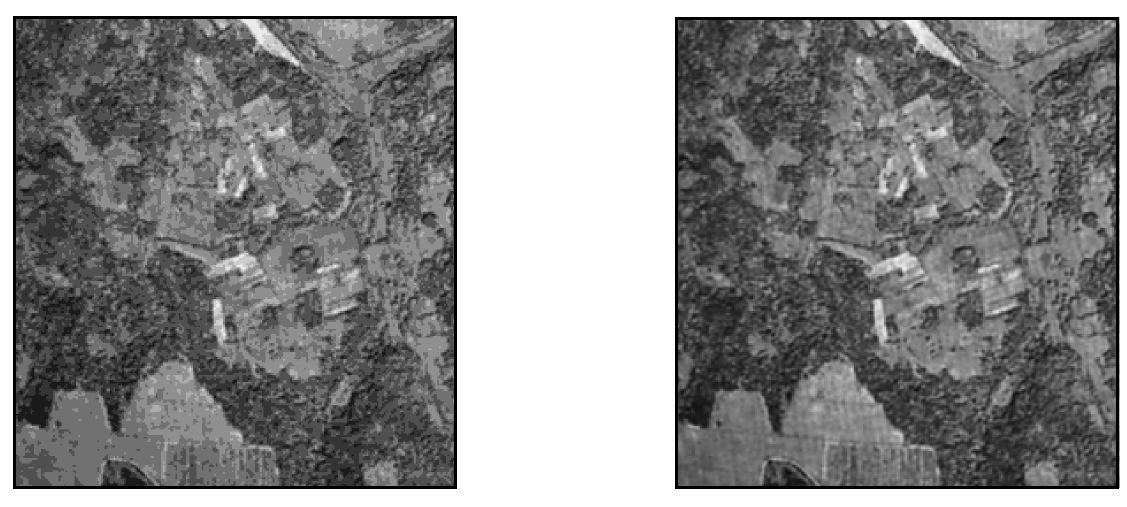
\includegraphics[width=.8\textwidth]{Fuentes_datos/Resolucion_radiometrica.png}
\caption{\small Dos imagenes con distinta resoluci�n radiom�trica (de izquierda a derecha, 8 y 256 niveles, respectivamente).}
\label{Fig:Resolucion_radiometrica} 
\end{figure}

	\item \textbf{Resoluci�n temporal}. Indica el tiempo que tarda el sensor en volver a tomar una imagen de una misma zona.  Tiene sentido en el caso de sensores orbitales, que funcionan por ciclos, y tras concluir este ciclo,  vuelven a comenzar la toma de im�genes en el mismo punto. En cada ciclo, el sensor cubre toda la superficie terrestre <<barriendo>> esta en franjas sucesivas.
	
	La resoluci�n temporal depende de la altura a la que se encuentra la plataforma que monta el sensor, as� como la resoluci�n espacial. Si el tama�o de las im�genes es reducido (GIFOV peque�o), las franjas son m�s estrechas y se requieren m�s para cubrir toda la superficie y volver a comenzar el ciclo, con lo que la resoluci�n espacial ser� menor.
\end{itemize}

Parece l�gico pensar que lo ideal en toda circunstancia ser�a disponer de im�genes procedentes de sistemas con altas resoluciones en cualquiera de las clases anteriores. De esta forma, tendr�amos im�genes con gran detalle espacial, espectral y radiom�trico, y actualizadas frecuentemente. No obstante, la tecnolog�a actual no dispone de elementos que ofrezcan resoluciones elevadas en todas las magnitudes del proceso, y en la creaci�n de los sensores se favorecen unas en detrimento de otras. Algunas resoluci�n presentan adem�s un cierto antagonismo, como hemos visto para las resoluciones espacial y temporal, con lo que no resulta viable que ambas sean elevadas simult�neamente.

As�, existen sensores con, por ejemplo, gran resoluci�n espacial, en los cuales la resoluci�n espectral no es tan elevada. Por el contrario, los sensores con mayor resoluci�n espectral no suelen ofrecer un nivel de detalle espacial tan elevado como los anteriores. En ocasiones, una misma plataforma puede montar a bordo varios sensores, de tal forma que el conjunto de ellos ofrezca informaci�n detallada de forma global, pero un �nico sensor no proporciona resoluci�n elevada en todas las variables.

Otro tipo de circunstancias relativas al sensor afectan igualmente a las resoluciones. Por ejemplo, aquellos sensores que trabajan con radiaciones de poca energ�a (en la regi�n de las microondas) y son de tipo pasivo requieren una amplia extensi�n para recoger la suficiente energ�a como para poder ser detectada por dicho sensor. Por esta raz�n, su resoluci�n espacial suele ser baja. 

A la hora de utilizar im�genes de teledetecci�n, debe considerarse qu� tipo de resoluci�n  resulta de mayor inter�s para el proyecto que se lleva a cabo, teniendo en cuenta la escala de trabajo o el objetivo final que se persigue con el an�lisis a realizar, entre otros factores. En base a esto, se escoger� uno u otro producto, que ser� el que ofrezca los valores de resoluci�n m�s adecuados en conjunto.

Si se pretende localizar elementos de peque�o tama�o, es imprescindible trabajar con altas resoluciones espaciales. Si lo que se desea es clasificar una serie de zonas en funci�n de sus caracter�sticas, la resoluci�n espectral debe ser alta, ya que, como veremos, se usa la informaci�n de todas las bandas para dar esa clasificaci�n, y un n�mero mayor de bandas dar� como resultado una mayor precisi�n.\index{Bandas}

De igual, modo, la detecci�n de cambios de intensidad en una banda hace necesario que se trabaje con una buena resoluci�n radiom�trica, pero si lo que se desea es estudiar esos cambios a lo largo de un periodo corto de tiempo, trabajar con un sensor con gran resoluci�n temporal se hace imprescindible.

En cada caso, las circunstancias particulares del trabajo condicionan la elecci�n de uno u otro sensor, puesto que, como se ha dicho, un �nico sensor no ofrece elevadas resoluciones en todas las variables.

La utilizaci�n simult�nea de datos de varios sensores en un proyecto es una alternativa en ciertos casos. Como veremos, existen t�cnicas que permiten combinar im�genes con alta resoluci�n espacial e im�genes con alta resoluci�n espectral, con objeto de obtener nuevas im�genes que combinen lo mejor de ambas y ofrezcan un nivel de detalle conjunto mayor. Estas t�cnicas realizan el proceso conocido como \emph{fusi�n de im�genes}, el cual trataremos en el apartado  \ref{Fusion_imagenes}, m�s adelante en este libro. \index{Im�genes!fusi�n de}\index{Fusi�n de im�genes}

Adem�s de lo anterior, un �nico sensor montado a bordo de un sat�lite puede operar en varios \emph{modos} distintos. Es habitual que un sensor multibanda pueda registrar tambi�n im�genes de una sola banda, recogiendo en ella la intensidad de la radiaci�n correspondiente a todo el espectro visible, de tal forma que genere una representaci�n visual real. Estas se suelen representar habitualmente en escala de grises, resultando una imagen en blanco y negro.

Las im�genes de este tipo se conocen como \emph{pancrom�ticas}\footnote{El t�rmino \emph{pancrom�tico} deriva de la fotograf�a cl�sica, conoci�ndose as� al tipo de pel�cula sensible a todas las longitudes de onda del visible. Por similitud de conceptos, se emplea el t�rmino tambi�n para hacer referencia a las im�genes digitales monobanda generadas por sensores seg�n lo comentado anteriormente}, y suelen tener mayor resoluci�n espacial, por lo que pueden emplearse para la fusi�n de im�genes se�alada anteriormente. As�, un mismo sensor provee todos los datos necesarios para llevar a cabo ese proceso, tanto la imagen de gran resoluci�n espacial (la pancrom�tica) como la de gran resoluci�n espectral (la imagen multibanda).
\index{Im�genes!pancrom�ticas}

\subsection{Principales sensores y productos}

El n�mero de diferentes productos provenientes de la teledetecci�n es muy elevado en la actualidad. Ahora que ya conocemos los fundamentos del proceso y las principales caracter�sticas de un sistema de teledetecci�n, es interesante mostrar un peque�o resumen de los principales productos disponibles. En ocasiones, desconocer la existencia de productos adecuados puede suponer la realizaci�n incorrecta o de modo ineficaz de un proyecto SIG, y dada la gran variedad existente, esto sucede con frecuencia. 

A continuaci�n se relacionan algunos de los sistemas de teledetecci�n principales y las caracter�sticas de sus productos.

\begin{itemize}
	\item \textbf{LANDSAT} \cite{webLandsat}. Se trata de un programa completo de adquisici�n de datos mediante teledetecci�n, que ha lanzado hasta la fecha un total de siete sat�lites entre 1972 y 1999. Por ello, el volumen de datos recogido es enorme, y lo convierte en una de las fuentes de datos m�s ricas  de entre las existentes en la actualidad. \index{Landsat}

	El �ltimo sat�lite, LANDSAT 7, tiene una �rbita helios�ncrona y una resoluci�n temporal de 16 d�as. A bordo de �l se monta el sensor ETM+\footnote{Enhanced Thematic Mapper Plus}, que permite la obtenci�n de im�genes pancrom�ticas con resoluci�n de 15 metros, e imagenes multibanda con resoluci�n de 60 metros. El sensor recoge un total de 8 bandas, y el tama�o de la imagen es de 170 $\times$ 183 km.

	Los sensores TM\footnote{Thematic Mapper} y MSS \footnote{Multispectral Scanner} se montan a bordo del sat�lite LANDSAT 5, todav�a en funcionamiento y con una resoluci�n temporal de 16 d�as. El sensor TM ofrece im�genes multibanda de 7 bandas con resoluci�n de 30 metros, excepto en la banda del infrarrojo t�rmico, donde la resoluci�n es de 120 metros. Las im�genes tienen un tama�o de 185 $\times$ 172 km.\index{TM (sensor)}\index{MSS(sensor)}
	\item \textbf{IKONOS} \cite{webIkonos}. Este sat�lite, lanzado en 1999, monta un sensor con resoluci�n de 1 metro para im�genes pancrom�ticas y 4 metros para im�genes multibanda (4 bandas). Las im�genes cubren una �rea de 11 $\times$ 11 km y el sat�lite tiene una resoluci�n temporal de entre 3 y 5 d�as.\index{IKONOS}
	\item \textbf{SPOT}\footnote{Satellite Pour l' Observation de la Terre} \cite{webSPOT}. Un conjunto de sat�lites lanzados inicialmente por la agencia espacial francesa, con especial �nfasis en la recogida de informaci�n relativa a variables ambientales. De los cinco puestos en �rbita, dos siguen actualmente en funcionamiento. El �ltimo de ellos, lanzado en 2002, monta el sensor HRG con capacidad de producir im�genes pancrom�ticas con resoluci�n entre 2,5 y 5 metros, e im�genes multibanda con resoluci�n de 10 metros. El periodo de revisita es de entre 1 y 4 d�as.
	Es de destacar que el sensor permite inclinaciones de hasta 27\degree respecto al nadir hacia ambos lados, por lo que puede cubrir una banda m�s ancha y tomar im�genes fuera del �rea determinada en cada instante por la �rbita.\index{SPOT}\index{Satellite Pour l' Observation de la Terre}
	\item \textbf{QuickBird}. \cite{webQuickbird}. Ofrece im�genes en pancrom�tico y multibanda (azul, verde, rojo e infrarrojo cercano). Las primeras tiene una resoluci�n de 60 cm y las multibanda de 2,4 metros, aunque combinando las dos ofrece im�genes en color con 60 cm de resoluci�n. 
	La �rbita del sat�lite es helios�ncrona y la resoluci�n temporal var�a entre los 3 y 7 d�as. Cada imagen cubre una superficie de 16,5 $\times$ 16,5 km.\index{QuickBird}
	\item \textbf{Aqua y Terra}. Dos sat�lites lanzados por la NASA dentro de un proyecto de �mbito internacional para la observaci�n de la Tierra. Cada uno de ellos monta una serie de diversos sensores, que recogen informaci�n relativa al ciclo hidrol�gico (en el caso del Aqua) y la superficie terrestre (en el caso del Terra). Entre estos sensores cabe destacar el MODIS, a bordo de ambos, o el ASTER, a bordo del sat�lite Terra. ASTER \footnote{Advanced Spaceborne Thermal Emission and Reflection Radiometer} recoge informaci�n en 14 bandas distintas, con una resoluci�n entre 15 y 90 metros, mientras que MODIS\footnote{Moderate Resolution Imaging Spectroradiometer} es un sat�lite de menor resoluci�n espacial (250, 500 o 1000 metros seg�n la banda ), 36 bandas y una resolucion temporal de 1 a 2 d�as. \index{Aqua}\index{Terra}\index{NASA}\index{ASTER}\index{MODIS}

	Adem�s de los datos directos de los sensores, se proporcionan de forma gratuita numerosos productos derivados, lo que lo convierte en una fuente de datos de primer orden para un gran n�mero de aplicaciones, especialmente las relacionadas con el estudio del medio, la vegetaci�n, etc. En la direcci�n Web \cite{webModisData} pueden obtenerse tanto datos originales como productos derivados.
	\item \textbf{NOAA--AVHRR}\footnote{Advanced Very High Resolution Radiometer}. Se encuentra principalmente enfocado al estudio de los oc�anos, aunque sus datos pueden aplicarse en muchos m�s estudios. El sensor tiene una resoluci�n de 1,1 km, y proporciona im�genes de 5 bandas en las regiones del infrarrojo y el visible. La resoluci�n temporal es de medio d�a, produciendo una imagen nocturna y otra diurna.\index{NOAA-AVHRR}
	\item \textbf{RADARSAT}. Desarrollado por la Agencia Espacial Canadiense, monta un radar de apertura sint�tica (SAR), y su principal prop�sito es el control de las variaciones ambientales y de los recursos naturales. M�s informaci�n en \cite{webRADARSAT}.\index{RADATSAT}\index{Radar de Apertura Sint�tica}\index{SAR}
	\item \textbf{ERS--1 y ERS--2}. Desarrollados por la Agencia Espacial Europea. Al igual que el anterior, ambos est�n pensados para la observaci�n medioambiental, y montan tanto sensores activos como pasivos. M�s informaci�n en \cite{webERS2}.\index{ERS--1}\index{ERS--2}
	\item \textbf{SRTM}. La misi�n SRTM\footnote{Shuttle Radar Topography Mission} es un proyecto internacional de gran envergadura destinado a la creaci�n de una cobertura de elevaciones a nivel mundial. Utilizando sensores basados en radar montados sobre una lanzadera espacial, se realiz� un vuelo global de la superficie terrestre a lo largo de 11 d�as, recogiendo el relieve de todas las zonas situadas entre los 56 grados sur y los 60 grados norte de latitud. La resoluci�n de los datos obtenidos es de un segundo de arco (aproximadamente 30 metros), aunque solo se encuentran disponibles para Estados Unidos, siendo de unos 90 metros en el resto de zonas. Los datos SRTM se pueden descargar gratuitamente en \cite{webSRTMDownload}. M�s informaci�n sobre el proyecto puede encontrarse en \cite{webSRTM}. \index{SRTM}\index{Shuttle Radar Topographic Mission}
\end{itemize}

\section{Cartograf�a impresa. Digitalizaci�n}

\index{Digitalizaci�n}

La primera fuente de cartograf�a de la que se dispon�a en las etapas iniciales de los SIG era la  cartograf�a impresa. No se trataba de elementos creados pensando en su utilizaci�n dentro de un SIG y, de hecho, su estructura no es, como veremos, la m�s adecuada para ser incorporados como datos de trabajo en un SIG. Se trata, por tanto, de una clara fuente secundaria de datos espaciales. Aun as�, esta fuente era la fuente principal de informaci�n cartogr�fica disponible entonces, y su uso ha sido desde esos tiempos una constante dentro del �mbito SIG.

A pesar de que hoy en d�a disponemos de otras fuentes cartogr�ficas, la cartograf�a impresa sigue siendo b�sica para trabajar con un SIG, ya que existe mucha informaci�n que todav�a solo se encuentra en este formato. De una u otra forma, es probable que un proyecto SIG implique en alg�n punto de su desarrollo la necesidad de recurrir a cartograf�a impresa y tratar esta para su inclusi�n dentro de un SIG.

Cuando hablamos de cartograf�a impresa, no hay que pensar �nicamente en mapas o planos, sino tambi�n en im�genes tales como fotograf�as a�reas, las cuales, dependiendo de su antig�edad, pueden encontrarse disponibles tan solo en formato impreso, como hemos visto. Mientras que resulta posible adquirir estas en formato digital cuando se trata de fotograf�as m�s actuales, la tomadas por m�todos anal�gicos correspondientes a vuelos m�s antiguos solo pueden adquirirse por regla general como un producto impreso.

Los procesos que permiten obtener un producto digital a partir de esas im�genes son costosos en tiempo y dinero, y es por ello que no todos los proveedores de estas ofrecen la posibilidad de adquisici�n de un producto digital. En esta secci�n veremos esos procesos, tanto si partimos de un mapa o plano como si partimos de una imagen o cualquier otro documento impreso que pueda contener informaci�n cartogr�fica, susceptible de ser convertida en una o varias capas seg�n se requieren para el trabajo en un SIG.

Ya conocemos los dos modelos de datos con los que trabajamos en un SIG: el modelo r�ster y el modelo vectorial. Tanto mapas como fotograf�as a�reas pueden servir como fuente de informaci�n para crear o bien capas r�ster o bien capas vectoriales, ya que la informaci�n que contienen puede de igual modo representarse seg�n uno u otro modelo (debe recordarse que, como se mencion� en el cap�tulo \ref{Tipos_datos}, puede convertirse una capa r�ster en vectorial y viceversa mediante algoritmos que detallaremos m�s adelante en este libro).\index{Conversi�n!r�ster--vectorial}

Un mapa o plano sobre un soporte impreso, sin embargo, dista considerablemente de ese concepto de capa con el que trabajamos en un SIG. Suele contener informaci�n sobre distintas variables, tales como carreteras, elevaci�n, n�cleos urbanos, uso de suelo, y todas ellas en un �nico elemento cartogr�fico. Esas variables, que en un SIG manejar�amos como capas independientes, se presentan como un conjunto que, seg�n el uso que queramos darle, va a ser mucho m�s conveniente disgregar en base a esas distintas variables.

Si pensamos en una fotograf�a a�rea, esta puede considerarse como una simple imagen dentro de un SIG, y como vimos en el cap�tulo \ref{Tipos_datos}, las im�genes se adaptan al modelo de representaci�n r�ster. Por otra parte, en esa imagen existir�n elementos tales como carreteras, r�os o �rboles, los cuales se representan mejor seg�n el modelo vectorial. En funci�n de qu� informaci�n nos interese tener dentro de un SIG o el modelo de representaci�n preferente que queramos manejar, las operaciones que debemos llevar a cabo ser�n unas u otras.

Este conjunto de operaciones posibles se conocen como de \emph{digitalizaci�n}, y en funci�n de la forma en que se desarrollen podemos distinguir los siguientes tipos:

\begin{itemize}
	\item Digitalizaci�n autom�tica 
	\item Digitalizaci�n manual
\end{itemize}

\index{Digitalizaci�n!tipos}

En la digitalizaci�n autom�tica, el sistema (inform�tico o mec�nico) se encarga de generar los elementos digitales que ya podremos incorporar a un SIG, ahorrando trabajo al operador al automatizar la tarea. Este tipo de digitalizaci�n es muy habitual para el caso de obtener un resultado r�ster mediante el proceso de \emph{escaneo}\index{Escaneo}. Tambi�n resulta posible automatizar la digitalizaci�n para el caso vectorial, aunque requiere cierta labor por parte del operario y no es un proceso tan sencillo, pudiendo obtenerse resultados desiguales. 

La digitalizaci�n manual requiere por parte del operario una definici�n expl�cita de los elementos a crear, y es por ello �nicamente adecuada para obtener un resultado vectorial, traz�ndose las entidades (sean estas puntos, l�neas o pol�gonos) manualmente mediante alg�n sistema que permita esa introducci�n de datos. 

La elecci�n de uno u otro tipo de digitalizaci�n no depende solo del tipo de capa que se desee obtener. Tanto la digitalizaci�n manual como la autom�tica, tienen cada una de ellas su propias ventajas. En el caso r�ster la opci�n manual no es viable, pero al digitalizar un mapa para obtener una capa vectorial puede ser interesante optar por una o otra metodolog�a en funci�n de las circunstancias. 

La digitalizaci�n manual es mucho m�s costosa y su resultado es muy variable en cuanto a su precisi�n espacial, ya que depende en gran medida de la experiencia del operario y de las condiciones de este (cansancio, circunstancias personales, etc.). Por el contrario, e independientemente del operario, el reconocimiento de las entidades es altamente fiable (si se trata de un mapa, este ha sido dise�ado para ser interpretado por una persona, por lo que esta reconocer� sus elementos sin dificultad y con total fiabilidad). 

Asimismo, un proceso autom�tico, en caso de proceder de forma correcta, tendr� una exactitud absoluta y <<clonar�>> con absoluta fidelidad los elementos del mapa impreso. Esto resulta una ventaja a la hora de obtener una gran precisi�n, pero impide que en el proceso de digitalizaci�n se puedan corregir errores existentes en el documento original. Un operario puede advertir esos errores y corregirlos a medida que digitaliza. Un sistema autom�tico, por el contrario, no puede.
 
\subsection{Digitalizaci�n manual}
\label{Digitalizacion_manual}\index{Digitalizaci�n!manual}

La digitalizaci�n manual es la forma m�s b�sica de crear informaci�n digital a partir de un documento cartogr�fico impreso. Un operario trabaja directamente sobre la fuente cartogr�fica y su trabajo se traduce en la creaci�n de una nueva capa, gracias a la utilizaci�n de un equipo que es capaz de convertir su trabajo en la informaci�n necesaria para crear dicha capa.

En el modelo de representaci�n r�ster, los elementos b�sicos son las celdas, que forman una malla regular que puede presentar un numero muy elevado de estas. Una definici�n manual de las caracter�sticas de cada una de esas celdas resulta inviable, por lo que la digitalizaci�n de un documento cartogr�fico impreso para la obtenci�n de una capa r�ster a partir de ella de forma manual no es factible.

Por el contrario, se puede realizar con cierta sencillez la digitalizaci�n de una entidad vectorial, trazando la forma de esta o, en caso de ser una entidad de tipo punto, sencillamente indicando su localizaci�n. Cuando el n�mero de entidades es elevado, el proceso puede llevar tiempo y ser tedioso, pero en todo caso sigue resultando una forma sencilla y accesible de crear una capa vectorial a partir de otra fuente de datos.

Para llevar a cabo ese trazado de la entidad, se necesita emplear alg�n equipo que recoja la informaci�n introducida por el operador. Existen dos alternativas principales: utilizar un equipo especializado dise�ado espec�ficamente para la digitalizaci�n, o bien digitalizar utilizando las funciones de edici�n de un GIS, realizando todo el proceso dentro de este y sin m�s herramientas que el propio ordenador y un dispositivo se�alador como el rat�n.

\subsubsection{Con equipo especializado (\emph{heads--down})} \label{heads-down}

\index{Heads--down}

La forma tradicional de proceder a la digitalizaci�n manual de entidades es utilizando equipos y perif�ricos expresamente dise�ados para llevar a cabo esta tarea. La \emph{tableta digitalizadora} (Figura \ref{Fig:Tableta_digitalizadora}) es la herramienta fundamental para este trabajo.\index{Tableta digitalizadora}

\begin{figure}[!hbt]   
\centering
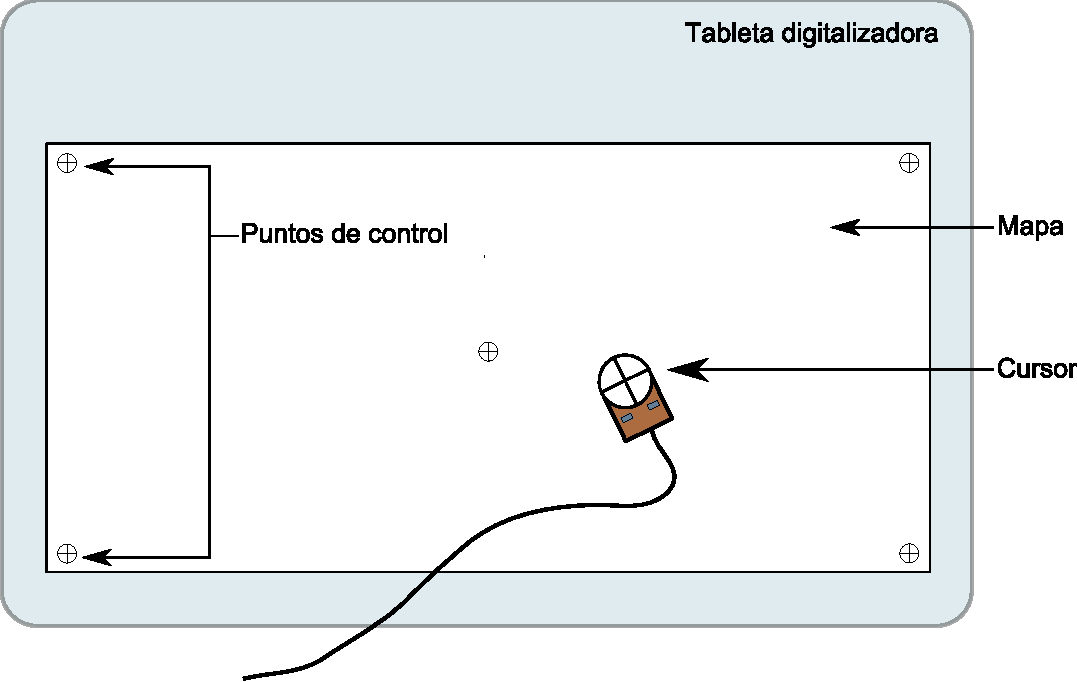
\includegraphics[width=.8\textwidth]{Fuentes_datos/Tableta_digitalizadora.pdf}
\caption{\small Esquema de una tableta digitalizadora y los elementos del proceso de digitalizaci�n.}
\label{Fig:Tableta_digitalizadora} 
\end{figure}

Se trata de una superficie plana a modo de atril, sobre la cual se sit�a el documento cartogr�fico a digitalizar, y sobre este se van trazando las distintas entidades con un cursor. Este cursor registra los movimientos del operario, convirtiendo las posiciones del cursos en coordenadas reales, que son las que van a constituir la entidad digitalizada. El trabajo del operario consiste en seguir con el cursor las formas de las distintas entidades, como si las estuviera calcando, de modo que indique al sistema las geometr�as que se quieren definir.

El proceso de digitalizaci�n implica los siguientes pasos \cite{Heywood1998Longman}:

\begin{itemize}
	\item \textbf{Registro}. La etapa fundamental del proceso, que garantiza que las coordenadas de las entidades digitalizadas sean correctas. El mapa se ha de adherir a la tableta de modo firme, normalmente con cinta adhesiva u otro medio similar, y se�alar en �l unos \emph{puntos de control} de coordenadas conocidas. Ser� en base a estos como se calcularan las restantes coordenadas de las entidades que el operario defina mediante el cursor. Habitualmente se utilizan como puntos de control las esquinas y alg�n punto central del mapa. Es importante que en el proceso de registro el mapa no presente dobleces o deterioros que puedan inducir errores en el c�lculo de coordenadas posteriores.\index{Puntos!de control}
	\item \textbf{Digitalizaci�n}. De entidades puntuales, lineales y poligonales.
	\item \textbf{Asignaci�n de atributos}. A cada una de las entidades digitalizadas se le a�aden sus correspondientes propiedades. Este paso no se realiza ya con la tableta digitalizadora.
	En el caso m�s general, estos atributos se introducen manualmente con el teclado o se toman, por ejemplo, de una base de datos. Un caso particular, no obstante, es el de la digitalizaci�n de curvas de nivel. Una vez que estas han sido digitalizadas, no es necesario asignar valores individualmente a cada una de las lineas, ya que entre ellas existe una relaci�n que puede aprovecharse para simplificar el establecimiento de una cota correspondiente a cada una. Estableciendo la elevaci�n de una y la direcci�n en que la elevaci�n aumenta, pueden sistem�ticamente asignarse elevaciones a las curvas que aparecen seg�n se avanza en dicha direcci�n. Los SIG m�s populares presentan habitualmente herramientas que facilitan este proceso.
\end{itemize}

Esta forma de digitalizar se conoce como <<cabeza abajo>> (\emph{heads--down}), en referencia a la posici�n del operario a la hora de trabajar sobre la tableta.

Se distinguen dos formas principales de registro de puntos:

\begin{itemize}
	\item \textbf{Manual}. El usuario debe ir marcando uno por uno todos los puntos que desee incorporar a la entidad digitalizada. Por ejemplo, para el caso de una l�nea, debe ir deteniendo el rat�n regularmente en aquellos puntos que considere de inter�s, y sobre ellos pulsando los botones del cursor para indicar al sistema que ha de registrar dichos puntos.
	\item \textbf{Semiautom�tica}. El operario simplemente desliza el cursor definiendo la forma de los entidades, y el propio sistema se encarga de almacenar puntos regularmente seg�n un intervalo de tiempo definido. Esto permite un ahorro de tiempo considerable y una correcta densidad de puntos recogidos para cada entidad.	
\end{itemize}

Las tabletas digitalizadoras son elementos caros, motivo por el cual se tiende a favorecer en la actualidad la digitalizaci�n en pantalla, que presenta adem�s otra serie de ventajas adicionales, como seguidamente veremos.
 
\subsubsection{En pantalla (\emph{heads--up})}

\index{Heads--up}

La otra forma de digitalizar elementos es utilizando las capacidades de edici�n de un SIG. Estas capacidades son heredadas de las aplicaciones de dise�o asistido por ordenador (CAD)\index{CAD}, y permiten <<dibujar>> en la pantalla del ordenador entidades y formas tales como los puntos, l�neas y rectas que constituyen los objetos en el modelo de representaci�n vectorial.

En este proceso se parte igualmente de un capa base, generalmente una imagen, y bas�ndose en ella se van definiendo los objetos, <<dibuj�ndolos>> sobre la pantalla, una vez m�s como si se calcara aquello que puede visualizarse en dicha imagen. El hecho de que un SIG nos permita tener varias capas simult�neamente y visualizarlas a voluntad, facilita el proceso de digitalizaci�n. Tambi�n lo facilita el poder tener varias im�genes sobre el fondo (cada una de ellas como una capa individual), de modo que podemos cubrir un �rea m�s amplia que la de una simple hoja de mapa o una �nica imagen.

En este proceso, no partimos en realidad de un documento cartogr�fico anal�gico, pues ya ha sido necesario digitalizarlo de alguna forma para incorporarlo en un SIG. El proceso es una digitalizaci�n de las entidades como tales, pero la informaci�n ya ha de estar en formato digital, aunque no en el modelo de representaci�n vectorial, sino en el modelo r�ster. Por ello, puede utilizarse como capa de partida una imagen originalmente en formato digital o bien una imagen originalmente en formato impreso. En este ultimo caso, la imagen ha debido digitalizarse previamente mediante un proceso de \emph{escaneo}, el cual se tratar� en la siguiente secci�n.

En la figura \ref{Fig:Digitalizacion_en_pantalla} puede verse un ejemplo de la digitalizaci�n de una imagen en pantalla.

\begin{figure}[!hbt]   
\centering
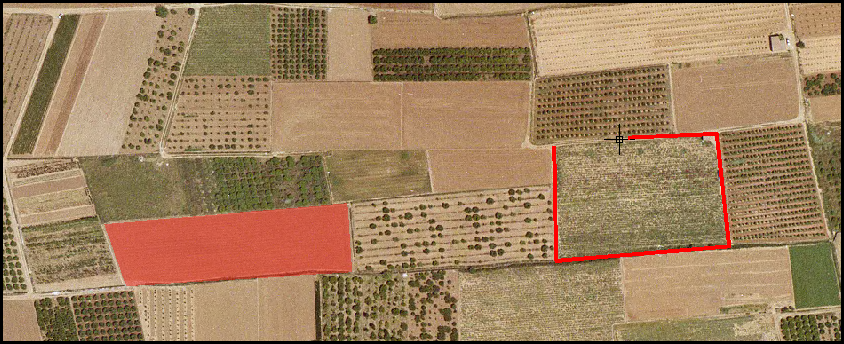
\includegraphics[width=.8\textwidth]{Fuentes_datos/Digitalizacion_en_pantalla.png}
\caption{\small Digitalizaci�n en pantalla. En rojo, pol�gono ya digitalizado. Las lineas rojas indican un nuevo pol�gono, actualmente en edici�n}
\label{Fig:Digitalizacion_en_pantalla} 
\end{figure}

En la figura, sobre una imagen a�rea en color se digitalizan las distintas parcelas que pueden distinguirse en esta. Del mismo modo, pueden digitalizarse curvas de nivel en un mapa escaneado, u otras entidades tales como r�os, lagos o v�as de comunicaci�n sobre una fotograf�a a�rea, entre muchas otras. La digitalizaci�n en pantalla puede incluso utilizarse teniendo como base no una imagen, sino capas de cartograf�a vectorial o cualquier capa de datos que aporte alg�n tipo de informaci�n que pueda delinearse con las mismas herramientas de edici�n.

La digitalizaci�n en pantalla se conoce tambi�n como digitalizaci�n <<cabeza arriba>> (\emph{heads--up}), ya que el operador centra su atenci�n en la pantalla, con una postura bien distinta a la que se tiene al trabajar con una tableta digitalizadora.

Frente a dicho trabajo con tableta digitalizadora, la digitalizaci�n en pantalla tiene las siguientes ventajas:

\begin{itemize}
	\item \textbf{Menor coste}. No se requiere equipo especializado de alto coste, ya que basta con un ordenador personal. 
	\item \textbf{Posibilidad de dividir el trabajo}. Cuando se trabaja con un mapa sobre una tableta digitalizadora, este mapa no puede ser utilizado por otro operario. Sin embargo, el uso de una capa digital dentro de un SIG como base para la digitalizaci�n, permite que varios operarios trabajen con ella simult�neamente y se repartan el trabajo.
	\item \textbf{Posibilidad de correcci�n y edici�n precisa}. Las mismas capacidades que se usan para trazar las distintas entidades puede emplearse para corregir o modificar estas una vez que estas ya han sido digitalizadas (Figura \ref{Fig:Correccion_digitalizacion}), resultando esto en un proceso de digitalizaci�n m�s flexible.
	\item \textbf{Posibilidad de ampliaci�n}. Para cartograf�as de baja calidad, puede ser dif�cil obtener precisi�n si se trabaja directamente sobre el mapa, as� como si los elementos a digitalizar son peque�os, requiri�ndose del operador un esfuerzo visual adicional. Las capacidades que tiene todo SIG para ampliar una imagen (\emph{zoom}) permiten superar esta dificultad y trabajar a distintas escalas seg�n la precisi�n del trabajo a realizar o las caracter�sticas de los objetos digitalizados.
	\item \textbf{Mayor precisi�n}. La capacidad de resoluci�n del ojo humano es mucho menor que la resoluci�n de las im�genes (v�ase m�s adelante el apartado \ref{Condiciones_digitalizacion}). Esto, unido a lo mencionado en el punto anterior, permite aprovechar mejor la informaci�n de la fuente original, y que los resultados obtenidos en la digitalizaci�n de esta sean m�s fieles a ella.
	\item \textbf{Mayor comodidad para el operario}. La postura del operario es m�s adecuada cuando se digitaliza sobre la pantalla, permitiendo unas mejores condiciones. Esto que se traduce en menor cansancio y ello indirectamente comporta resultados m�s precisos.
\end{itemize}

\begin{figure}[!hbt]   
\centering
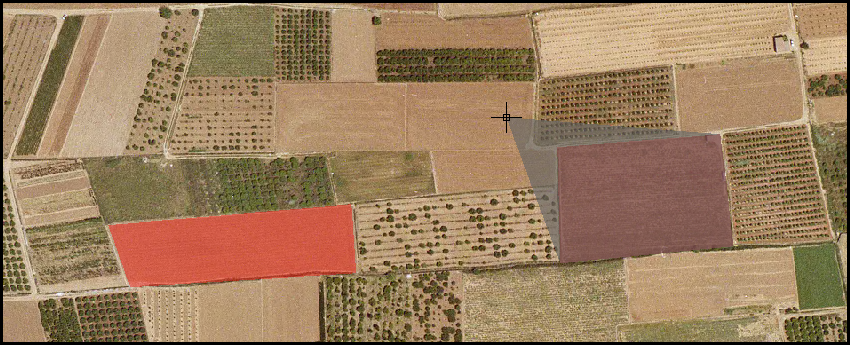
\includegraphics[width=.8\textwidth]{Fuentes_datos/Correccion_digitalizacion.png}
\caption{\small Correcci�n de entidades con las funciones de edici�n de un SIG. El pol�gono de la derecha se encuentra en edici�n, siendo modificado uno de sus v�rtices.}
\label{Fig:Correccion_digitalizacion} 
\end{figure}

Para conocer con m�s detalle las capacidades b�sicas de edici�n de un SIG, as� como las restantes capacidades que contribuyen a su vez a facilitar la labor de edici�n, cons�ltese el capitulo \ref{SIGs_escritorio}.

\subsection{Digitalizaci�n autom�tica}\index{Digitalizaci�n!autom�tica}

La digitalizaci�n autom�tica limita el trabajo del operario, ya que este no es responsable directo de definir las propiedades de los elementos que se digitalizan. Este tipo de digitalizaci�n es la  habitual en el caso de generar una capa r�ster, aunque tambi�n pueden obtenerse capas vectoriales procesando de modo autom�tico cartograf�a impresa. 

Este segundo caso, no obstante, requiere una cartograf�a en condiciones especiales, no siendo adecuada para todo tipo de mapas. En caso de no presentarse esas condiciones, los resultados de la digitalizaci�n no son �ptimos, y requieren posteriormente un gran trabajo de correcci�n y supervisi�n.

\subsubsection{Escaneo}
\label{Escaneo}

\index{Escaneo}

El escaneo es el proceso de digitalizaci�n que convierte una imagen impresa (anal�gica) en una imagen digital \cite{Jackson1991Longman}. El resultado de este proceso es, por tanto, y desde el punto de vista de un SIG, una capa r�ster. Pueden escanearse tanto mapas como fotograf�as a�reas, operando en ambos casos de un modo similar y con las mismas consideraciones, pues el objeto del proceso es el mismo: la conversi�n del documento impreso en un documento digital que pueda utilizarse dentro de un SIG o cualquier otro software tal como, por ejemplo, un software de tratamiento de im�genes.

El dispositivo fundamental para realizar este proceso es el \emph{esc�ner}. Este se compone de una \emph{cabeza} sobre la que se monta un sensor, y un soporte sobre el que se desplaza o bien la cabeza o bien el documento a escanear, de tal modo que durante el proceso de escaneo esta recorre todo el documento, recogiendo la informaci�n de toda su extensi�n.\index{Esc�ner}

Este proceso de \emph{barrido} se realiza en una �nica ocasi�n, aunque dispositivos m�s antiguos pueden hacerlo en tres ocasiones a la hora de escanear documentos en color. Aunque lo habitual es la creaci�n de una imagen en color, tambi�n  pueden obtenerse im�genes en blanco y negro o en escala de grises.

Aunque existen esc�neres espec�ficamente dise�ados para el trabajo con documentos cartogr�ficos, estos son dispositivos muy especializados y de muy elevado coste. Los esc�neres m�s gen�ricos, pensados para el trabajo con todo tipo de im�genes y para todo tipo de usos, pueden no obstante emplearse de igual modo para escanear tanto mapas como im�genes a�reas con resultados aceptables, utiliz�ndose con frecuencia.

Existen tres tipos principales de esc�neres:

\begin{itemize}
	\item \textbf{De sobremesa} (\emph{flat--bed}). Los habituales para el uso dom�stico o el escaneo de im�genes de peque�o formato, aunque tambi�n existen de mayor tama�o. El documento a escanear se sit�a sobre una placa de cristal bajo la que se desplaza la cabeza con el sensor. Puede verse uno de estos esc�neres en la figura \ref{Fig:Escaner_sobremesa}.\index{Flat--bed}
	\item \textbf{De tambor}. El mapa se sit�a sobre un tambor que rota, mientras que la cabeza se mantiene fija. La figura \ref{Fig:Escaner_tambor} muestro uno de estos esc�neres.
	\item \textbf{Alimentados}. El sensor se mantiene fijo y el documento se desplaza mediante un mecanismo de arrastre, de forma similar a como avanza el papel en una impresora dom�stica. Salvo que dispongan de mecanismos espec�ficos para corregir esta circunstancia, suelen presentar importantes distorsiones geom�tricas causadas por un desplazamiento impreciso del papel.
\end{itemize}

\begin{figure}[!hbt]   
\centering
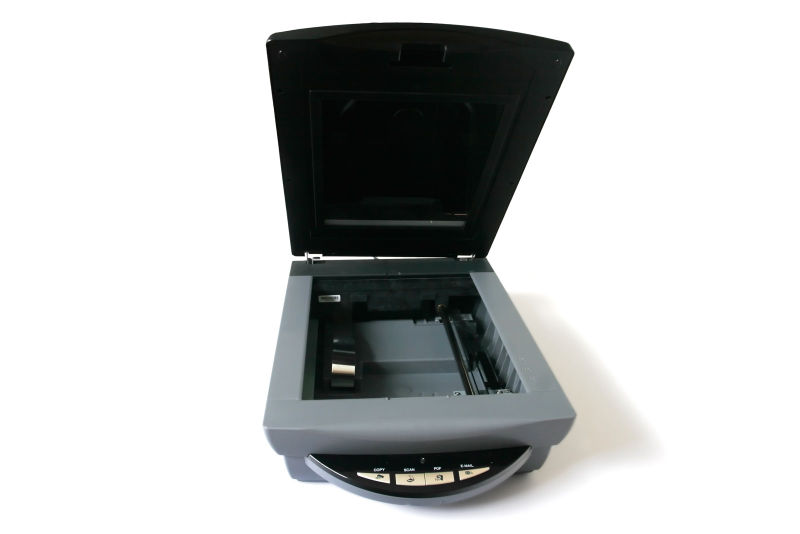
\includegraphics[width=.5\textwidth]{Fuentes_datos/Escaner_sobremesa.png}
\caption{\small Esc�ner de sobremesa (tomado de Wikipedia)}
\label{Fig:Escaner_sobremesa} 
\end{figure}

\begin{figure}[!hbt]   
\centering
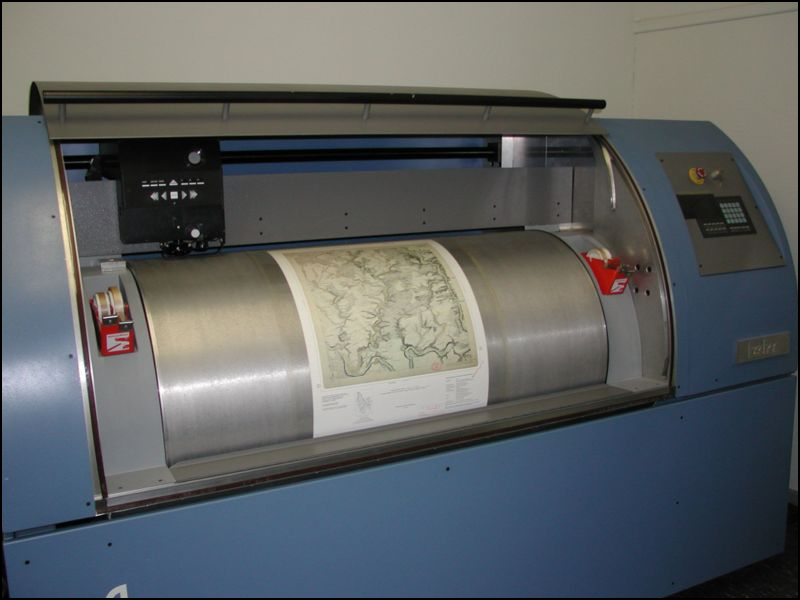
\includegraphics[width=.5\textwidth]{Fuentes_datos/Escaner_tambor.png}
\caption{\small Esc�ner de tambor (fotograf�a: Stefan Kuehn)}
\label{Fig:Escaner_tambor} 
\end{figure}

Los par�metros b�sicos que definen las caracter�sticas de un esc�ner son la resoluci�n espacial y la resoluci�n radiom�trica. La primera de estas de mide habitualmente en \emph{puntos por pulgada}\footnote{\emph{Dots per inch}(dpi)} y nos indica el n�mero de puntos (celdas) que el sensor es capaz de tomar por cada unidad de longitud sobre el papel. La resoluci�n radiom�trica, por su parte, indica la capacidad del sensor para distinguir entre dos colores distintos.\index{Dots per inch}\index{Resoluci�n!espacial}\index{Resoluci�n!radiom�trica}

A la hora de trabajar con documentos cartogr�ficos de cara a su posterior utilizaci�n en un SIG, tanto la resoluci�n espacial como la radiom�trica de los esc�neres habituales es en general m�s que suficiente, incluso en ocasiones en aquellos de uso dom�stico. No obstante, es habitual que se presenten distorsiones geom�tricas que suponen un problema importante a la hora de mantener la precisi�n cartogr�fica, y ello exige la utilizaci�n de equipos de mayor calidad si se requiere un resultado de alta precisi�n. Estos equipos no han de ser necesariamente de aquellos pensados para el trabajo con cartograf�a, sino que pueden ser de uso gen�rico, siempre, eso s�, que sean de la calidad necesaria.

La velocidad del esc�ner es otro par�metro importante, pues la preparaci�n de una base de datos cartogr�fica a partir de cartograf�a anal�gica puede llevar un tiempo considerable si el volumen de datos es elevado, ya que el proceso de escaneo es laborioso y requiere de cierto tiempo. El rendimiento del esc�ner y la velocidad a la que puede digitalizar una imagen dada est� en relaci�n directa con la resoluci�n espacial. Un esc�ner posee una resoluci�n nominal (en dpi), que es la resoluci�n m�xima a la que puede trabajar (el detalle m�ximo que puede recoger). No obstante, puede ajustarse la resoluci�n de trabajo en funci�n de las necesidades, y una resoluci�n mayor siempre lleva asociado un tiempo de proceso mayor, ya que el volumen de informaci�n generado es mayor, as� como el detalle que ha de registrarse.\index{Resoluci�n!nominal de un escaner}

Para cada documento existe una resoluci�n �ptima de escaneo en funci�n de las caracter�sticas de este. Esta resoluci�n debe elegirse teniendo en cuenta que el volumen de datos aumenta a medida que empleamos una mayor resoluci�n, buscando un equilibrio adecuado entre ese volumen de datos resultante y la cantidad de informaci�n que recogemos. Asimismo, se ha considerar igualmente el tiempo necesario para escanear el documento, tal como se dijo anteriormente.

El par�metro base es la relaci�n entre el tama�o de p�xel (la longitud real que representa el ancho de un p�xel sobre el terreno) y el tama�o de este p�xel en la imagen (lo que mide esa longitud en el mapa). Las resoluciones habituales utilizadas para el escaneo de fotograf�as a�reas var�an entre los 100 dpi ($\approx 250 \mu m$ cada punto sobre el mapa) y 2500 dpi (($\approx 10 \mu m$ cada punto sobre el mapa) \cite{Welch1996Onward}. Por ejemplo para una resoluci�n de 300 dpi, se tiene:

\begin{equation}
300 \mathrm{dpi} = \frac{300\mathrm{filas}}{2,54 \mathrm{cm\; de\; mapa}} = 118,11 \mathrm{filas/cm\; de\; mapa}
\end{equation}

En un cent�metro cuadrado se tienen $118,11^2\approx13950$ puntos.

Si trabajamos, por ejemplo, con un mapa a una escala 1:50000, tenemos que la distancia real que representa el alto de cada fila es

\begin{equation}
\frac{50000 \mathrm{cm}}{118,11 \mathrm{filas}} = 4,24 \mathrm{metros}/\mathrm{fila}
\end{equation}

Es decir, cada p�xel del mapa representa sobre el terreno un cuadrado de lado 4,24 metros.\index{Pixel}

Con c�lculos similares podemos calcular para cada posible resoluci�n el espacio real que representa, y elegir esta en funci�n del detalle que necesitemos. Como regla general, debe tratar de trabajarse con una resoluci�n que garantice que los objetos que resultan de inter�s de la imagen (por ejemplo, aquellos que van a digitalizarse despu�s manualmente mediante una digitalizaci�n en pantalla con esa imagen) sean distinguibles con claridad. 

En el caso de im�genes a�reas, la resoluci�n de estas medida en pares de lineas por mil�metro puede ser superior y permitir escanear a mayor resoluci�n, aunque ello no es estrictamente necesario, y debe una vez m�s buscarse el equilibrio entre las ventajas y los inconvenientes de trabajar con una resoluci�n m�s elevada.

En \cite{Welch1996Onward} puede encontrarse informaci�n m�s detallada sobre la elecci�n de una resoluci�n �ptima en el escaneo de im�genes a�reas.

Para el caso de mapas, no deben olvidarse los fundamentos cartogr�ficos en base a los cuales se ha creado dicho mapa, que fueron detallados en el cap�tulo \ref{Fundamentos_cartograficos}. Trabajando con una resoluci�n m�s elevada no hace necesariamente que estemos incorporando m�s informaci�n, ya que esta puede no existir en el mapa original. Tendr�amos un volumen de datos m�s elevado que el necesario para recoger toda la informaci�n del mapa.

Una diferencia fundamental entre escanear una hoja de un mapa y una imagen a�rea es la diferencia de tama�o. Los mapas suelen tener tama�os mucho mayores que los de un esc�ner com�n, lo cual obliga a utilizar equipos de gran formato o, en la mayor�a de los casos, contratar servicios de escaneo especializados, ya que estos equipos tiene un coste muy elevado. 

Una soluci�n distinta en el caso de mapas de gran tama�o es el escaneo de la hoja por partes y la posterior uni�n de las distintas partes. En este caso, es necesario asegurarse de que las partes son coherentes entre s� en lo que respecta a las condiciones bajo las que se realiza el escaneo, as� como garantizar que las distintas partes se solapan para que no existan zonas sin datos en la imagen resultante. Adem�s de esto, el solape facilita la localizaci�n de puntos comunes presentes entre partes contiguas, lo que ayuda en la composici�n de todas las partes para dar lugar al resultado global.

Otra diferencia entre trabajar con mapas e im�genes es la relativa al tipo de soporte. En el caso de mapas, el documento original se encuentra siempre impreso en papel. En el caso de fotograf�as a�reas puede presentarse tanto en papel como en diapositiva. Los esc�neres est�n preparados para capturar la imagen tanto por \emph{reflexi�n} (cuando se trabaja con un documento en papel) como por \emph{transmisi�n} (cuando se trabaja con una diapositiva o cualquier otro soporte transparente), por lo que ambos tipos de fuentes pueden utilizarse indistintamente para generar una imagen digital, siendo esta diferencia menos relevante a efectos pr�cticos.

Por �ltimo, un aspecto clave en el escaneo de cartograf�a es la asignaci�n de coordenadas a la capa resultante. Cuando utilizamos una tableta digitalizadora, debemos definir los \emph{puntos de control}, que son los que establecen la referencia geogr�fica en base a la cual se calculan las coordenadas de los elementos que digitalizamos con el cursor. En el caso de escanear un mapa o una fotograf�a a�rea, esa informaci�n est� presente en el mapa en forma de marcas fiduciales o una ret�cula con coordenadas impresas, pero no se digitaliza como tal.\index{Puntos!de control}\index{Marcas fiduciales}

Si simplemente escaneamos el documento, se digitaliza la marca fiducial o la etiqueta que indica las coordenadas, pero tan solo como una imagen, y no como un dato aprovechable por el SIG para otras tareas. En esta imagen, un operador puede ver las coordenadas de un punto, pero si realizamos un proceso de digitalizaci�n vectorial en pantalla utilizando esa imagen, el SIG no tiene forma de calcular las coordenadas de los puntos que introducimos, pues carece de una referencia.

Para que una imagen procedente del escaneo de un documento impreso tenga plena validez y utilidad dentro de un SIG, es necesario a�adirle informaci�n sobre la localizaci�n en el espacio del �rea representada en dicho documento. Este proceso se denomina \emph{georreferenciaci�n}.\index{Georreferenciaci�n}

La georreferenciaci�n es un proceso tratado dentro de este libro en el apartado \ref{Rectificacion}, puesto que no es puramente un proceso que forme parte de la adquisici�n de datos, sino un tratamiento a aplicar una vez que el proceso de digitalizaci�n ha sido realizado. No obstante, es necesario recalcar de nuevo la importancia vital de este proceso, ya que sin �l no resulta posible aprovechar el resultado del escaneo dentro de un SIG.

\subsubsection{Vectorizaci�n autom�tica}

\index{Vectorizaci�n}

La vectorizaci�n autom�tica es un proceso completamente distinto al de escaneo, y no es tan habitual en el �mbito de los SIG, principalmente debido a la mayor dificultad que entra�a. Como resultado de este proceso, se obtiene una capa vectorial, pero, a diferencia de la vectorizaci�n manual, el operario no tiene que se�alar los puntos de estas o trazar los contornos de las entidades.

Existen distintos procesos de vectorizaci�n autom�tica, entre los que distinguiremos los siguientes:

\begin{itemize}
	\item Vectorizaci�n en base a una imagen digital, por reconocimiento de entidades en un software apropiado.
	\item Vectorizaci�n mediante dispositivos espec�ficos que trabajan sobre un documento anal�gico.
\end{itemize}

En el primer caso, partimos de una imagen digital, que puede proceder o no de un proceso de escaneo. Sobre esta imagen se aplican algoritmos que identifican de modo autom�tico las distintas entidades y crean los correspondientes objetos vectoriales. 

El mayor inconveniente de esta t�cnica es que requiere que la imagen tenga unas condiciones especiales, pues de otro modo es dif�cil que esos algoritmos de identificaci�n den resultados correctos. En ocasiones pueden crear entidades donde estas no existen o bien ignorar algunas por no ser capaces de detectarlas, as� como crear entidades de forma y tama�o incorrectos. El trabajo de digitalizaci�n por parte del operario desaparece, pero es necesario un trabajo posterior de comprobaci�n y correcci�n, que en funci�n de las caracter�sticas de la imagen de partida puede ser importante.

Esta forma de vectorizaci�n autom�tica es, al igual que la georreferenciaci�n, un proceso a llevar a cabo sobre la imagen. Por esta raz�n, no se trata en este cap�tulo sino en el cap�tulo \ref{Procesado_imagenes} dedicado al tratamiento de im�genes. Igualmente, el cap�tulo \ref{Creacion_capas_vectoriales}, dedicado a la conversi�n entre capas r�ster y vectoriales, incluye informaci�n acerca de procesos de vectorizaci�n autom�tica, con particular atenci�n a la conversi�n de un mapa escaneado en una capa vectorial de curvas de nivel.

La otra forma de digitalizaci�n es totalmente diferente y no se realiza en el ordenador, sino en un perif�rico externo a este, tal como una tableta digitalizadora o un esc�ner. El dispositivo en cuesti�n es m�s similar a un esc�ner que a una tableta digitalizadora, pero su comportamiento imita al de un operario trabajando sobre esta �ltima.

Para ello, dispone de sensores luminosos y de l�ser\index{Laser@L�ser} que buscan las l�neas en la imagen y las recorren, almacenando las coordenadas por las que han pasado en el recorrido. De este modo, se genera un resultado vectorial en lugar de uno r�ster. El barrido de la imagen no es sistem�tico como el de un esc�ner, sino que <<sigue>> las l�neas que est�n presentes en la imagen, y que son las que van a digitalizarse. 

Al igual que con la digitalizaci�n autom�tica, las condiciones de la imagen de partida son b�sicas para obtener resultados de calidad. En un mapa, por ejemplo, las l�neas habitualmente se ven interrumpidas por etiquetas (por ejemplo, para indicar la altura de una curva de nivel), o bien se dibujan en trazo punteado, o bien puede aparecer alguna mancha sobre ellas. Este tipo de elementos dificultan o incluso imposibilitan el correcto funcionamiento del dispositivo, ya que este no puede seguir las l�neas adecuadamente, obteni�ndose resultados de poca calidad.\index{Curva!de nivel}

\subsection{Digitalizaci�n o creaci�n de capas a partir de coordenadas. Geocodificaci�n}
\label{Geocodificacion}

\index{Geocodificaci�n}

Junto a las formas de digitalizaci�n que acabamos de ver, existe una forma a�n m�s b�sica: la digitalizaci�n directa de valores y coordenadas, sin necesidad alguna de dispositivos especializados o elementos gr�ficos. En este tipo de digitalizaci�n no existe un mapa o documento cartogr�fico, sino simplemente una serie de datos espaciales expresados de forma alfanum�rica que son susceptibles de convertirse en una capa y emplearse as� dentro de un SIG.

Este proceso se conoce como \emph{geocodificaci�n} \cite{Davis2003Geoinfo} e implica la asignaci�n de coordenadas a puntos de inter�s, los cuales pueden ser de naturaleza muy variada. Asimismo, la procedencia de estos datos tambi�n puede ser muy variada, y en general muchas formas de trabajo en campo dan lugar a datos que, a�n no estando originalmente dispuestos sobre mapas, s� que pueden emplearse como base para la creaci�n de capas. Algunos ejemplos son los siguientes:\index{Geocodificaci�n}

\begin{itemize}
	\item Muestreos de campo tales como la medici�n de parcelas en un inventario forestal. Cada parcela tiene una coordenada correspondiente a su centro, y los �rboles medidos se referencian con un rumbo y una direcci�n en base a ese centro.
	\item Calicatas para an�lisis de suelo
	\item Levantamientos topogr�ficos con instrumentaci�n tanto anal�gica como digital. Existe un conjunto de instrucciones y procedimientos denominado COGO (\emph{COordinate GeOmetry}), que facilita el trabajo con datos en forma de distancias y �ngulos, de forma que las mediciones efectuadas a lo largo de un recorrido empleando un equipo tal como una estaci�n total, un teodolito o un nivel con una mira, todos ellos pueden posteriormente convertirse con sencillez a coordenadas mediante la incorporaci�n al SIG de ese conjunto de valores.\index{Coordinate GeOmetry (COGO)}
	\item Coordenadas en las que han sucedido alg�n tipo de sucesos. Por ejemplo, la geocodificaci�n de localizaciones en las que han tenido lugar sucesos criminales permite posteriormente el an�lisis de su distribuci�n y el establecimiento de pol�ticas de seguridad m�s acordes con el escenario real.
	\item Coordenadas de cierto tipo particular de elementos, tales como elementos arquitect�nicos, �rboles singulares, paradas de autob�s. Estas permiten la localizaci�n r�pida de estos y una f�cil catalogaci�n, adem�s de, en conexi�n con otras capas, c�lculos como, por ejemplo, la forma m�s r�pida de desplazamiento hasta uno de ellos.
	\item Coordenadas correspondientes a otras formas de codificaci�n espacial. Sistemas de localizaci�n espacial tales como c�digos postales o, por ejemplo, los sistemas de indexaci�n espacial CGDG o \emph{c-squares} \cite{WebCSquares}, pueden todos ellos vincularse a coordenadas geogr�ficas, de tal modo que a cada uno de los c�digos de estos sistemas se le asigne una de tales coordenadas.\index{CGDG}\index{c-squares}
	\item En la actualidad, Internet est� viendo aparecer tendencias relacionadas con la asignaci�n de una localizaci�n geogr�fica a muchos de sus elementos. As�, puede a�adirse a una p�gina Web informaci�n sobre el emplazamiento donde ha sido creada, o a�adirla a una fotograf�a digital que forme parte de un �lbum alojado en otra Web. Los datos con los que trabajamos en la Web (textos, im�genes, etc.) llevan asociados a su vez otros datos (metadatos) con informaci�n sobre su localizaci�n. El proceso de a�adir estos metadatos\index{Metadatos} se conoce como \emph{geotagging}.\index{Geotagging}
\end{itemize}

Todos estos datos presentan en com�n que, recogidos de un modo u otro, conforman un conjunto de coordenadas puntuales que habitualmente sirven para el trabajo fuera de un SIG y no llegan a incorporarse a este, o que al menos no est�n dispuestos en la forma habitual de capa con la que trabajamos en un SIG. 

En el caso de encontrarse en formato anal�gico, estos datos pueden digitalizarse mediante la simple introducci�n manual de coordenadas a trav�s del teclado o bien mediante alg�n sistema m�s espec�fico como el escaneo del documento y el empleo de alg�n software de reconocimiento de caracteres (OCR)\footnote{Optical Character Recognition}.\index{OCR}\index{Escaneo}

En el caso de encontrarse ya en formato digital, estos datos pueden presentarse como tablas en una hoja de c�lculo, datos asociados a otro dato de cualquier tipo (como en el caso del \emph{geotagging}) o incluso simples archivo de texto. Muchos SIG incorporan m�todos para leer estos archivos y despu�s utilizar las coordenadas que contienen con el fin de crear una nueva capa, en general de puntos.

Un caso particular de la creaci�n de puntos con coordenadas es la asignaci�n de direcciones dentro de n�cleos urbanos, tales como direcciones postales o c�digos postales. Estas direcciones son de especial importancia en el desarrollo de actividades dentro del entorno urbano, ya que es m�s habitual referirse al emplazamiento de un determinado elemento (por ejemplo, un comercio), en t�rminos de su direcci�n postal que en coordenadas espaciales tales como las que se manejan en un SIG.

La geocodificaci�n de estos elementos implica establecer una coordenada geogr�fica correspondiente a cada direcci�n postal. Al realizar este proceso, es frecuente la interpolaci�n de las coordenadas en las que se sit�an los distintas direcciones de una misma calle, ahorrando as� esfuerzos. Mediante esta forma de operar, conociendo los n�meros de los portales en ciertos puntos (habitualmente en cruces o n�meros de portal m�ltiplos de un valor dado) se pueden asignar coordenadas a los restantes portales si se asume que estos se distribuyen de forma homog�nea a lo largo de un tramo de calle, aplicando sencillos m�todos de interpolaci�n. La figura \ref{Fig:Geocodificacion} muestra un ejemplo de ello.\index{Interpolaci�n}

\begin{figure}
\centering
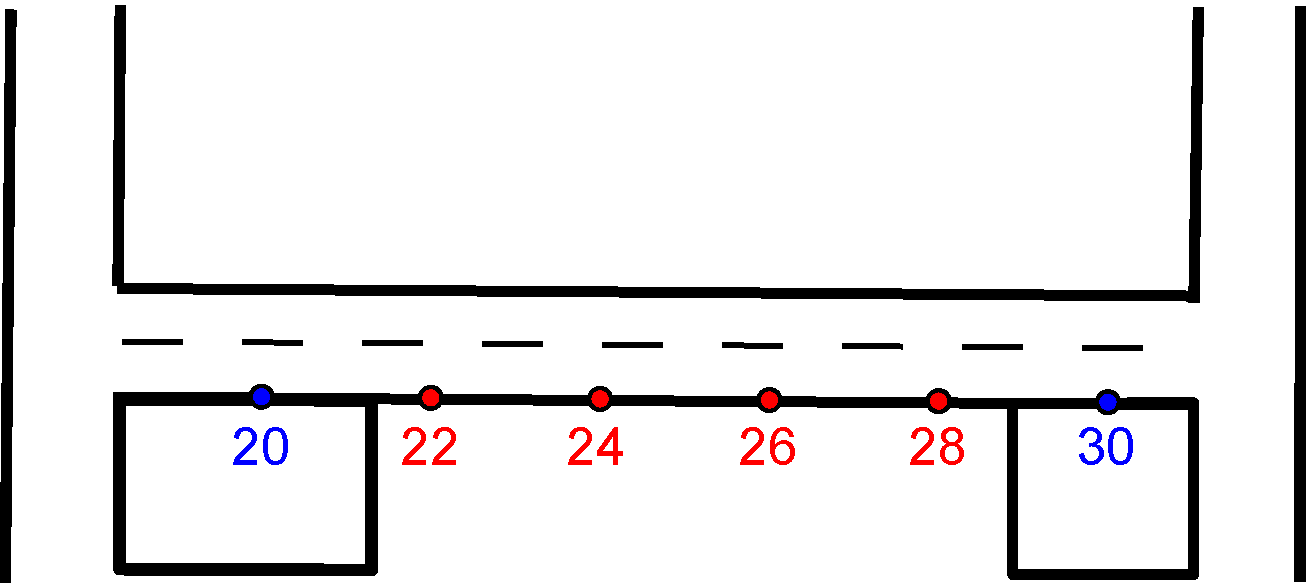
\includegraphics[width=.65\textwidth]{Fuentes_datos/Geocodificacion.pdf}
\caption{\small Interpolaci�n de direcciones. En azul, direcciones conocidas. En rojo, direcciones interpoladas.}
\label{Fig:Geocodificacion} 
\end{figure}

Esta pr�ctica, no obstante, no es del todo precisa, ya que asume que los edificios se encuentran equiespaciados, y por tanto son del mismo tama�o todos ellos, lo cual no sucede en la pr�ctica.  Adem�s de ello, el proceso presenta otras consideraciones particulares, tales como el hecho de que no en todos los pa�ses se sigue un mismo sistema de asignaci�n de direcciones postales, teniendo cada uno el suyo propio, que puede diferir en mayor o menor medida de lo que podr�a considerarse un sistema est�ndar. El supuesto habitual en que las direcciones pares se sit�an a un lado de la calle y las impares al lado contrario no resulta siempre cierto.

Otro aspecto a tener en cuenta es que el edificio se�alado con una direcci�n dada se identifica con una coordenada puntual, pero realmente ocupa una superficie \cite{WikipediaGeocoding}. Si esta es grande, puede presentar incluso varios puntos de acceso al mismo (o incluso accesos por varias calles distintas), con lo que la informaci�n que se recoge al geocodificar dicho edificio puede ser imprecisa e insuficiente.

Por todo ello, la interpolaci�n de direcciones permite una aproximaci�n v�lida para muchos usos, pero en aquellos casos en los que se requiera m�s precisi�n no pueden emplearse estas direcciones con total seguridad, ya que la exactitud de las coordenadas asociadas por el proceso de interpolaci�n puede variar notablemente seg�n sea la propia configuraci�n de los distintos edificios.

\subsection{Fotogrametr�a}
\label{Fotogrametria}

\index{Fotogrametr�a}

Un caso particular de digitalizaci�n lo encontramos en la \emph{fotogrametr�a}. En la definici�n cl�sica de \cite{Bonneval1972Eyrolles}, esta se define como la t�cnica para estudiar y definir con precisi�n la forma, dimensiones y posici�n en el espacio de un objeto cualquiera, utilizando medidas realizadas sobre una o varias fotograf�as. Esta definici�n no limita el alcance de la fotogrametr�a al �mbito de lo geogr�fico, y se utilizan sus principios en campos tales como la arqueolog�a o la documentaci�n de obras y monumentos, empleando para ello fotograf�as no a�reas, sino terrestres. Es la denominada \emph{fotogrametr�a terrestre}. No obstante, la rama de inter�s para este libro es la de la \emph{fotogrametr�a a�rea}, cuya base de trabajo tradicional son las fotograf�as a�reas.

Esta clase de fotogrametr�a viene, pues, ligada �ntimamente a los inicios de la teledetecci�n, cuando los sensores modernos que hemos estudiado antes en este mismo cap�tulo no se hab�an desarrollado, y los existentes (b�sicamente c�maras fotogr�ficas especialmente adaptadas a la toma de fotograf�as de tipo cartogr�fico) se montaban a bordo de aviones. Es por esta raz�n que tradicionalmente existe una conexi�n indudable entre ambas materias, no existiendo una frontera clara entre ambas, y se consideran en ocasiones como t�rminos id�nticos que hacen referencia la disciplina global de obtenci�n de im�genes y tratamiento de estas.

Hist�ricamente, el t�rmino \emph{teledetecci�n} aparece con posterioridad, una vez que las t�cnicas de toma de im�genes avanzan y dan un gran salto cualitativo con la aparici�n de las im�genes satelitales y los sensores electro--�pticos que ya conocemos. Algunos autores engloban la fotogrametr�a dentro de la teledetecci�n, mientras que otros se refieren con el termino teledetecci�n a las tecnolog�as m�s actuales y las consideran disciplinas distintas aunque muy relacionadas. Junto con la fotogrametria a�rea aparece la fotogrametr�a espacial, encargada de operar sobre im�genes de sat�lite bajo unos principios similares.

Dentro de este libro entenderemos por teledetecci�n todo el conjunto de t�cnicas y operaciones de obtenci�n de im�genes (que ya conocemos), as� como las de tratamiento y posterior extracci�n de resultados a partir de estas (que iremos viendo en otros cap�tulos), obteni�ndose estos resultados sin necesidad de establecer contactos con los objetos a estudiar, como corresponde a la definici�n dada en el apartado correspondiente. Dentro de ese conjunto de operaciones que nos llevan desde las im�genes a los resultados, entendemos como parte de la fotogrametr�a aquellas que tienen relaci�n con la acepci�n original del t�rmino, es decir, aquellas que derivan de la medici�n de elementos.

La denominaci�n, no obstante, no es tan relevante, y s� lo es sin embargo comprender la importancia de ambas, particularmente dentro de este cap�tulo como t�cnicas de producci�n cartogr�fica. 

En lo que respecta a la fotogrametr�a, el proceso de \emph{restituci�n} es el que interesa principalmente para el contenido de este cap�tulo, pues ofrece como resultado nuevas capas de datos tanto bidimensionales como, especialmente, tridimensionales. As�, pueden obtenerse tanto las capas vectoriales digitalizadas que ve�amos por ejemplo en el apartado \ref{Digitalizacion_manual}, como directamente Modelos Digitales de Elevaciones a partir de im�genes.\index{Restituci�n}

En realidad, los procesos de digitalizaci�n que ya hemos visto son tambi�n parte de la fotogrametr�a digital, y es habitual encontrarlos en los textos al uso sobre esta. Tambi�n lo son los procesos de rectificaci�n que se han citado en su momento, y que analizaremos en detalle m�s adelante en el cap�tulo \ref{Procesado_imagenes}. Como puedes ver, todas las t�cnicas est�n sumamente relacionadas, y las divisiones que hacemos pueden ser unas u otras en funci�n del enfoque que se d� para su estudio

Todas estas operaciones se llevan a cabo con una \emph{estaci�n fotogram�trica}, que comprende las herramientas necesarias para llevar estas a cabo (algunas, como los esc�neres, ya las conocemos). En funci�n del tipo de herramientas y t�cnicas distinguimos los siguientes tipos de fotogrametr�a, que representan a su vez la evoluci�n de la disciplina.\index{Estaci�n fotogram�trica}

\begin{itemize}
	\item Fotogrametr�a \textbf{anal�gica}. Basada en mediciones y procedimientos sobre im�genes anal�gicas
	\item Fotogrametr�a \textbf{anal�tica}. Basada en formulaciones matem�ticas y t�cnicas computacionales, permite obtener grandes precisiones.
	\item Fotogrametr�a \textbf{digital}. Basada en el trabajo con im�genes digitales dentro de un entorno computerizado.
\end{itemize}

El inter�s principal desde el punto de vista de los SIG es en la fotogrametr�a digital, ya que existe una gran relaci�n entre estos y las aplicaciones empleadas en dicho tipo de fotogrametr�a. Es en esta en la que pueden englobarse los procesos de digitalizaci�n que ya hemos visto, y no en las restantes formas m�s antiguas de fotogrametr�a. En la fotogrametr�a digital, la estaci�n fotogram�trica se articula sobre un ordenador en el cual se llevan a cabo los distintos procesos, no existiendo operaciones externas al mismo. As�, las im�genes se manejan dentro del ordenador y se visualizan a trav�s de �l, y la generaci�n de nueva cartograf�a tambi�n se produce de forma digital.

Esto no es muy diferente de lo que ve�amos en el caso de la digitalizaci�n en pantalla algunas paginas atr�s, pero el trabajo fotogram�trico engloba otros procesos adem�s de los que ya hemos visto. Uno de ellos es la generaci�n directa de cartograf�a de elevaciones, para la cual se requiere que el equipo empleado disponga de algunos elementos adicionales. Es decir, la estaci�n fotogram�trica digital es m�s compleja que un simple ordenador, un dispositivo de marcado (un rat�n) y un SIG, que eran los requisitos b�sicos para digitalizar en pantalla una imagen.

Una estaci�n fotogram�trica digital ha de tener, por ejemplo, capacidad para generar visualizaciones con sensaci�n de profundidad a partir de pares de im�genes, que son las que permiten la posterior digitalizaci�n de los elementos con sus elevaciones correspondientes. Los principios en los que se basan este tipo de visualizaciones son los mismos empleados en la fotogrametr�a no digital, fundamentados en la visi�n estereosc�pica. \index{Par estereosc�pico}

La visi�n tridimensional en el ser humano se basa en el hecho de que la imagen que ve cada ojo es ligeramente distinta a la del otro, lo cual permite al cerebro extraer informaci�n volum�trica y generar una verdadera visi�n tridimensional. En el caso de la fotogrametr�a, si en lugar de utilizar una �nica imagen a�rea o de sat�lite empleamos dos, cada una de ellas tomada desde un punto distinto, resulta posible recrear el efecto que ambas im�genes tendr�an para la reconstrucci�n tridimensional de la escena, y <<enga�ar>> al cerebro del observador para que este pueda observar la escena con volumen y profundidad.

Cuando se emplean im�genes de sat�lite, los pares se pueden obtener con aquellas plataformas y sensores que permiten variar el �ngulo de visi�n, de modo que en la misma pasada del sat�lite se toman im�genes de una zona desde distintos puntos. El sensor toma una imagen cenital y posteriormente, una vez ha superado la zona en su recorrido, toma una segunda imagen mirando <<hacia atr�s>>, la cual, combinada con la primera, permite el levantamiento del terreno y la realizaci�n de los procesos fotogram�tricos (Figura \ref{Fig:Par_estereo_satelite}).

\begin{figure}[!hbt]
\centering
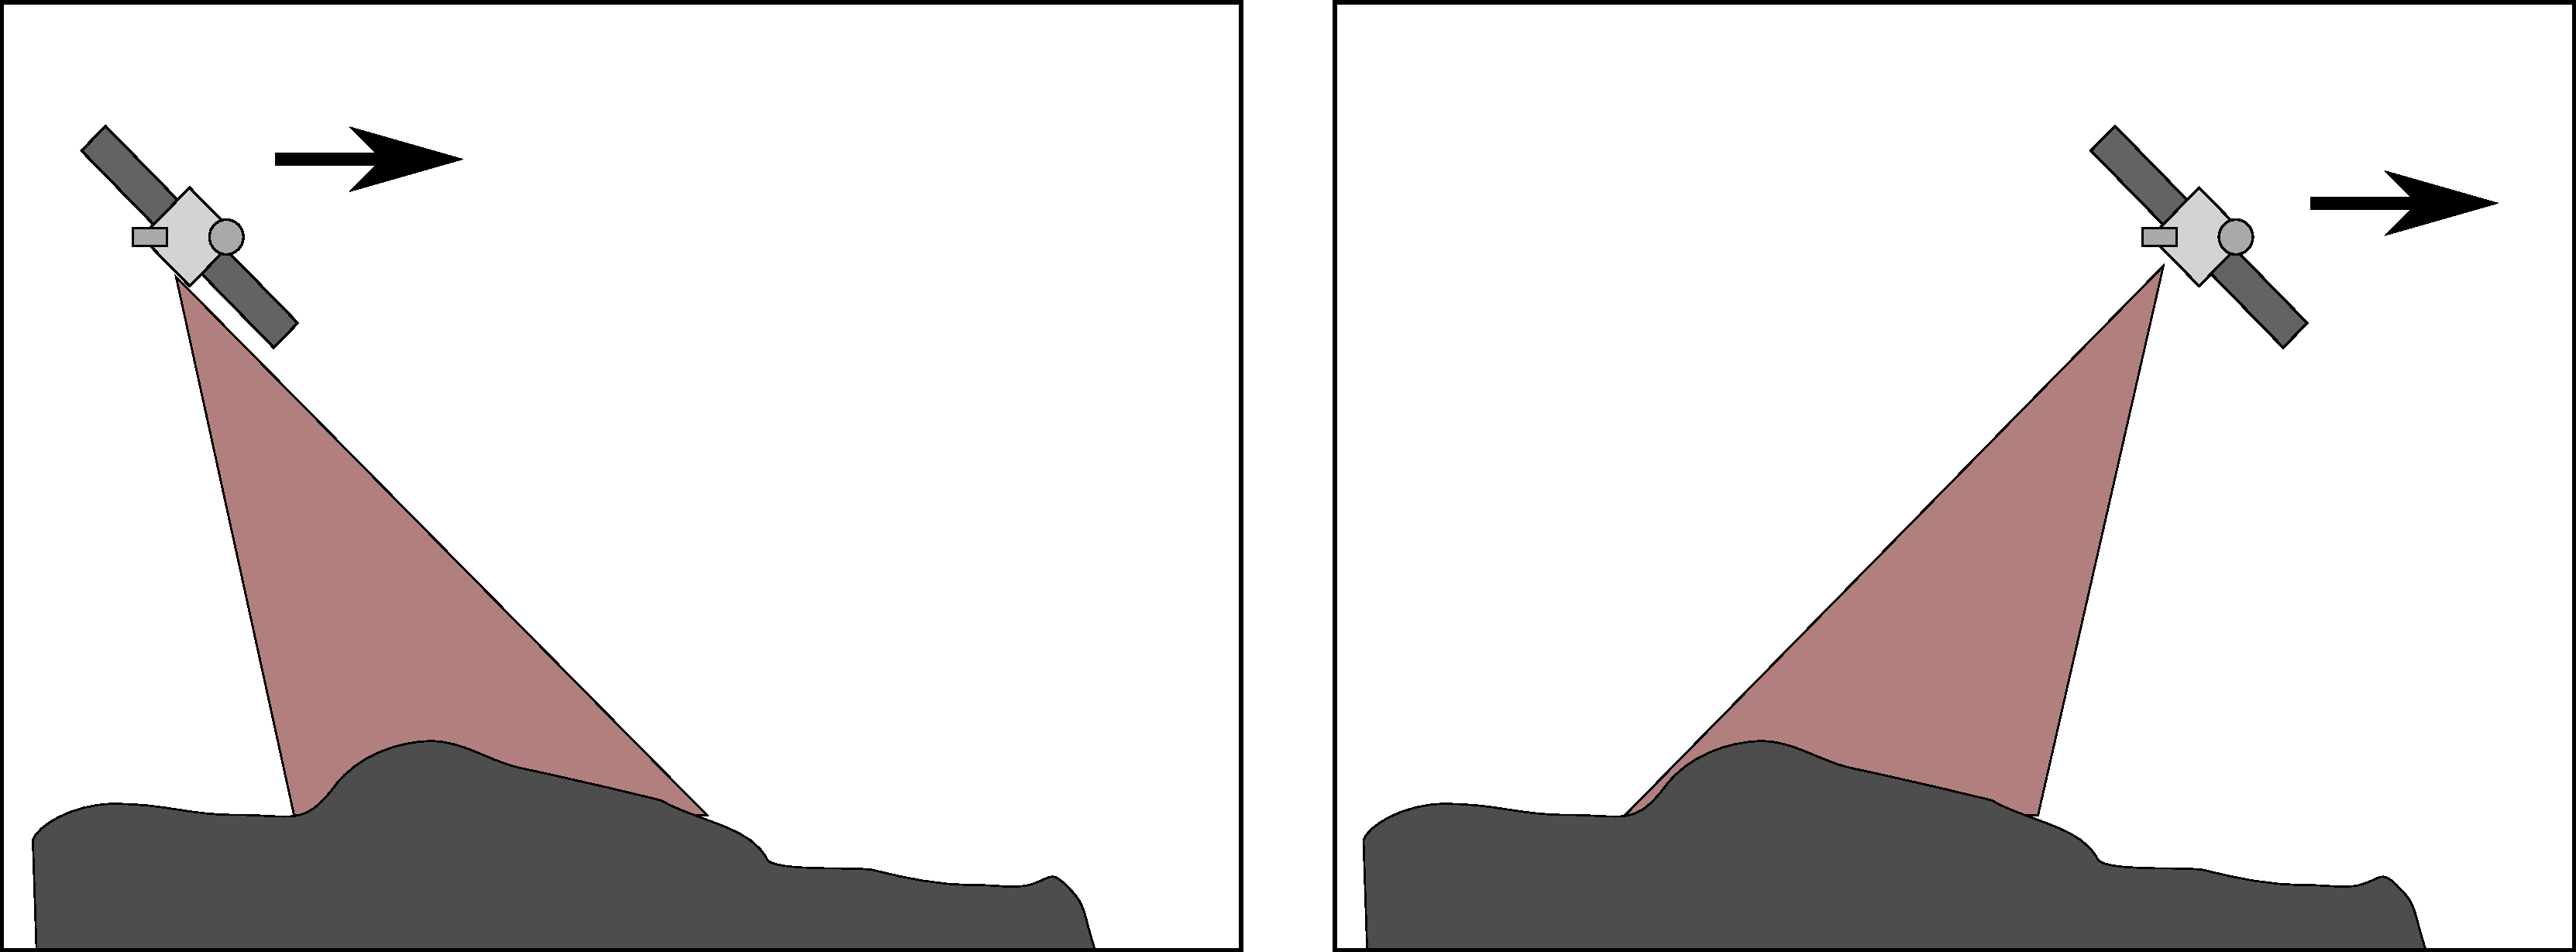
\includegraphics[width=.85\textwidth]{Fuentes_datos/Par_estereo_satelite.pdf}
\caption{\small Toma de pares de im�genes estereos�picas desde un sat�lite, mediante variaci�n del �ngulo de visi�n.}
\label{Fig:Par_estereo_satelite} 
\end{figure}

El sensor HRS que montan los sat�lites SPOT, o el sensor ASTER, ambos son capaces de tomar este tipo de im�genes. En la direcci�n Web \cite{webSPOTDEM} puede encontrarse informaci�n detallada sobre las cartograf�a de elevaciones generada a partir de pares de im�genes tomadas por el sat�lite SPOT, junto con algunas ilustraciones y animaciones explicativas al respecto. \index{SPOT}\index{ASTER}

Las formas de conseguir que el observador perciba la profundidad de la escena a partir de las im�genes son variadas, y van desde el uso de sencillos instrumentos �pticos o la generaci�n de anaglifos (im�genes que combinan la informaci�n del par estereosc�pico y que se han de observar con gafas con filtros distintos para cada ojo), hasta otras t�cnicas m�s complejas y elaboradas. En la fotogrametr�a no digital, el empleo de restituidores anal�ticos %como el mostrado en la figura \ref{Fig:Restituidor_analitico} 
ha sido la metodolog�a habitual. En la fotogrametr�a digital, este puede sustituirse por un equipo con dos monitores, cada uno de los cuales muestra una de las im�genes del par, y se emplean gafas especiales que son las encargadas de generar en el observador la sensaci�n de profundidad .\index{Anaglifos}

\begin{figure}
\centering
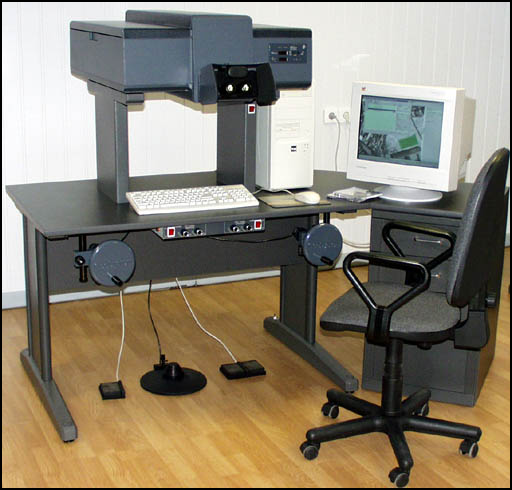
\includegraphics[width=.5\textwidth]{Fuentes_datos/Estacion_fotogrametrica_digital.png}
\caption{\small Estaci�n fotogram�trica digital.}
\label{Fig:Estacion_fotogrametrica_digital} 
\end{figure}

Adem�s de lo anterior, la estaci�n fotogram�trica digital dispone de perif�ricos espec�ficos tales como ratones 3D, o manivelas como las que presentan los restituidores anal�ticos, facilitando as� la adaptaci�n de los operarios a este tipo de estaci�n (Figura \ref{Fig:Estacion_fotogrametrica_digital}).

Por �ltimo el software que implementan, y que es el encargado de representar las im�genes y acoger el proceso de digitalizaci�n, suele ser espec�fico, y es frecuente que se distribuya como parte de toda una estaci�n fotogram�trica compuesta por los elementos rese�ados anteriormente. Algunos SIG incorporan progresivamente capacidades adaptadas de este tipo de programas, pero por el momento la labor fotogram�trica queda reservada para este tipo de aplicaciones espec�ficas, siendo el SIG tan solo un beneficiario directo de sus productos.

Para el lector interesado en saber m�s acerca de los distintos elementos de la fotogrametr�a, obras como  \cite{Lerma2002UPV} o \cite{Brito2002IME} son recomendables, esta �ltima disponible de forma libre. En la direcci�n Web \cite{webFotogrametriaUNEX} puede encontrarse otra excelente referencia libre en dos tomos sobre fotogrametr�a anal�tica y digital.

\subsection{Calidad de la digitalizaci�n}
\label{Condiciones_digitalizacion}

\index{Digitalizaci�n!calidad}

Uno de los aspectos m�s importantes del proceso de digitalizaci�n es la calidad del resultado obtenido, que debe tratar de ser lo m�s cercano posible a la calidad original de la informaci�n que se digitaliza, es decir, del mapa o imagen original. Independientemente de la precisi�n del equipo utilizado o la habilidad y experiencia del operario, la digitalizaci�n no es por completo perfecta, conteniendo siempre ciertas deficiencias y errores. 

Adem�s de los errores que puedan incorporarse en las distintas fases del proceso de digitalizaci�n (sea este del tipo que sea), hay que considerar que las fuentes originales a digitalizar tambi�n pueden incluir los suyos propios. As�, el proceso de escaneado puede incorporar distorsiones geom�tricas, pero es posible que el mapa o fotograf�a a�rea de partida tambi�n presente alguna distorsi�n como consecuencia de su deterioro, m�s patente cuanto m�s antigua sea esta. 

La informaci�n contenida en el documento cartogr�fico puede tambi�n contener elementos problem�ticos de cara a obtener un producto de calidad, que pueden ir desde l�neas borradas total o parcialmente a manchas en el propio mapa derivadas de su uso habitual \cite{Heywood1998Longman}.

Dentro de los errores que aparecen como consecuencia de la digitalizaci�n en s�, un tipo importante de ellos son las discrepancias y coincidencias imperfectas entre las distintas entidades, tal como las que se muestran en la figura \ref{Fig:Imprecisiones_digitalizacion}

\begin{figure}[!hbt]   
\centering
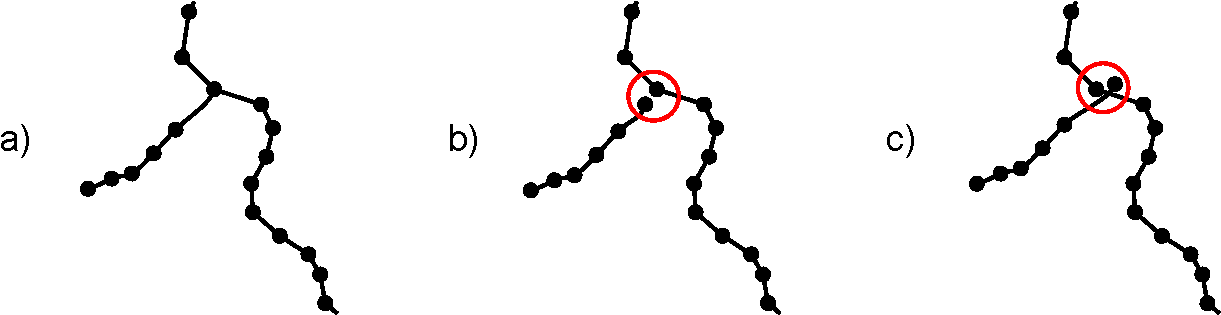
\includegraphics[width=.8\textwidth]{Fuentes_datos/Imprecisiones_digitalizacion.pdf}
\caption{\small Errores derivados del proceso de digitalizaci�n. a) Versi�n correcta, con nodos coincidentes. b) y c) Versiones con errores que causan una falsa desconexi�n entre las l�neas.}
\label{Fig:Imprecisiones_digitalizacion} 
\end{figure}

Estas imprecisiones son causantes de numerosos problemas, tales como la aparici�n de pol�gonos esp�reos en las operaciones de solape entre capas vectoriales, que veremos en el cap�tulo \ref{Operaciones_geometricas}.\index{Pol�gono!espureo}

Debido a esto, las capacidades de edici�n de los SIG incorporan funcionalidades que permiten evitar estos errores en el momento de la digitalizaci�n, ayudando al operario en su tarea y permiti�ndole alcanzar una exactitud y precisi�n imposible de lograr sin estas funcionalidades. Entre ellas, es especialmente importante el establecimiento de tolerancias y ajuste autom�tico en funci�n de ellas (esto se conoce con el t�rmino ingles \emph{snapping}), que ayudan a garantizar la coincidencia entre los distintos v�rtices. \index{Snapping}

De este modo, pol�gonos adyacentes o lineas que se cortan en un punto dado lo hacen con total exactitud. Dichos pol�gonos comparten exactamente el mismo lado con las mismas coordenadas exactas, o se cruzan en el mismo e id�ntico punto, y no �nicamente pasan por un punto cercano (pero distinto) definido con la precisi�n con la que el operador haya podido ajustar ambas entidades visualmente. La coincidencia no es solo visual, sino num�rica. La figura \ref{Fig:Snapping} muestra un ejemplo de la utilizaci�n de \emph{snapping} en un proceso de digitalizaci�n.

\begin{figure}
\centering
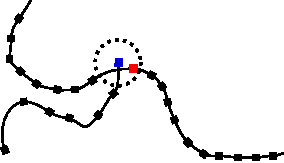
\includegraphics[width=.4\textwidth]{Fuentes_datos/Snapping.pdf}
\caption{\small Ajuste autom�tico mediante tolerancia(\emph{snapping}). El nodo azul representa el nodo en edici�n. La tolerancia de enlace queda marcada por el circulo punteado. Puesto que el nodo rojo de la l�nea preexistente se encuentra dentro de esa tolerancia, al a�adir el nuevo nodo (azul), este autom�ticamente se situar� en las coordenadas del nodo rojo, garantiz�ndose as� la coincidencia.}
\label{Fig:Snapping} 
\end{figure}

Mediante estas funcionalidades, el operador simplemente selecciona un punto, y el sistema digitalizador lo desplaza para que coincida con el punto existente m�s cercano, siempre que se encuentre a menos distancia que la tolerancia establecida de antemano.

El hecho de que exista una completa coincidencia es especialmente importante cuando la capa vectorial que se digitaliza contiene informaci�n topol�gica. La topolog�a exige que la coincidencia sea correcta y defina perfectamente la relaci�n entre las entidades. Para los ejemplos b) y c) de la figura \ref{Fig:Imprecisiones_digitalizacion}, las l�neas no est�n conectadas ya que no existe coincidencia en el nodo. Si los puntos est�n suficientemente cercanos, puede <<parecer>> que son coincidentes, pero el SIG no los detectar� como tales y no se podr� llevar a cabo ning�n an�lisis topol�gico con esas l�neas (por ejemplo, suponiendo que representan v�as de comunicaci�n y se quiere hacer un an�lisis de redes con ellas).

La digitalizaci�n de entidades en caso de querer recoger la topolog�a\index{Topolog�a} de las mismas debe obedecer una serie de reglas, a saber\cite{GrassDigitizing}:

\begin{itemize}
	\item Las l�neas deben cruzarse en nodos, en caso de que exista relaci�n (conexi�n) entre ellas.
	\item Las lineas que coinciden en un nodo com�n deben coincidir exactamente. Las funciones de \emph{snapping} se han de utilizar por ello durante la digitalizaci�n.
	\item Los lados comunes de los pol�gonos deben digitalizarse una �nica vez.
	\item Las �reas deben ser cerradas (el primer punto ha de coincidir exactamente con el �ltimo). Las funciones de \emph{snapping} o el cierre autom�tico de l�neas (asignar sistem�ticamente al �ltimo punto del contorno del pol�gono las coordenadas del primero) deben emplearse para ello.
\end{itemize}

Todos aspectos relativos a la calidad de datos, entre los cuales se incluyen las aspectos relativos a los errores del proceso de digitalizaci�n, se tratan con mayor profundidad en el cap�tulo \ref{Calidad_datos}.\index{Datos!calidad}


\section{GPS}
\label{GPS}

Uno de los hitos en la aparici�n de nuevas fuentes de datos geogr�ficos es la aparici�n de los \emph{Sistemas Globales de Navegaci�n por Sat�lite} (GNSS)\footnote{\emph{Global Navigation Satellite System}}, que permiten la obtenci�n de coordenadas geogr�ficas de un modo inmediato, con las consecuencias que esto tiene para su uso en actividades como la elaboraci�n de cartograf�a.\index{GNSS}\index{GPS}

En esencia, un GNSS es un sistema que permite conocer en todo momento y en cualquier punto del globo la localizaci�n exacta de dicho punto con un margen de error del orden de unos pocos metros o menos. Para ello, se basan en el env�o de se�ales entre un dispositivo situado en el punto concreto y una red de sat�lites, pudiendo establecerse la posici�n exacta mediante las caracter�sticas de dicha transmisi�n.

El ejemplo m�s extendido de un GNSS es el Sistema de Posicionamiento Global (Global Positioning System, o GPS)\footnote{El nombre completo del sistema es NAVSTAR--GPS (NAVigation SysTem And Ranging - Global Position System)}, originalmente puesto en funcionamiento por el Departamento de Defensa de los Estados Unidos. Actualmente, este es el �nico GNSS completamente operativo, aunque existen otros tales como el GLONASS ruso, el COMPASS chino o el \emph{Galileo} europeo, cuyo funcionamiento completo est� previsto a corto plazo. \index{GLONASS}\index{Galileo}\index{COMPASS}

\subsection{Fundamentos del sistema GPS}

El sistema GPS se divide en tres subsistemas o \emph{segmentos}:

\begin{itemize}
	\item \textbf{Segmento espacial}. Lo componen los sat�lites de la constelaci�n GPS (un total de 27, siendo 24 de ellos operativos y 3 de reserva), con los cuales se comunican las unidades receptoras, y en funci�n de los cuales puede triangularse la posici�n actual de estas.
	\item \textbf{Segmento de control}. Lo forman un conjunto de estaciones terrestres que controlan el funcionamiento de los sat�lites, pudiendo enviar se�ales a estos para modificar su comportamiento.
	\item \textbf{Segmento de usuarios}. Lo conforman los receptores GPS y todos los dispositivos que hacen uso de la se�al de los sat�lites para el c�lculo de posiciones.
\end{itemize}

\index{Segmentos!del sistema GPS}

Los sat�lites del segmento espacial emiten una se�al compleja cuyo contenido puede dividirse esencialmente en dos bloques de informaci�n:

\begin{itemize}
	\item \textbf{Se�ales empleadas para el c�lculo de distancias}. Estas incluyen dos c�digos: P(Precise) y C/A (Coarse/Aquisition). El segundo de ellos es el empleado habitualmente, ya que el primero se encuentra encriptado y est� pensado para uso militar, mientras que el C/A esta disponible para todos los usuarios.
	\item \textbf{Mensajes de navegaci�n}. Estos informan de la posici�n orbital del sat�lite (conocida como \emph{efem�ride}), y pueden asimismo contener informaci�n adicional referente al segmento espacial.
\end{itemize}

\index{Efem�ride}

Las se�ales para el c�lculo de distancias (en la terminolog�a GPS estas distancias se conocen como \emph{pseudodistancias}) se env�an mediante una onda portadora conocida como L1, correspondiente a una frecuencia de 1575,42 MHz . El c�digo P se env�a adem�s en una segunda portadora denominada L2, con una frecuencia de 1227,60 MHz.\index{Pseudodistancias}

El funcionamiento del sistema se basa en la triangulaci�n de la posici�n mediante las se�ales procedentes de un cierto n�mero de los sat�lites. Esta posici�n se calcula no �nicamente en sus coordenadas \emph{x} e \emph{y}, sino tambi�n en \emph{z}, es decir en elevaci�n. El sistema GPS emplea como sistema geod�sico de referencia el WGS84 \cite{WGS84}. La precisi�n en el c�lculo de la elevaci�n es menor que la correspondiente a las restantes coordenadas, aunque tambi�n es de utilidad y puede emplearse en aplicaciones que van desde levantamientos y replanteos a usos en tiempo real como el c�lculo de elevaci�n en vuelos \cite{Graas1991Navigation}.\index{WGS84}

La posici�n de los sat�lites es conocida en todo momento, y los propios sat�lites informan de ella a los receptores a trav�s de los mensajes de navegaci�n. En base a esas posiciones orbitales, el proceso de triangulaci�n que se lleva a cabo en el sistema GPS no se basa en el trabajo con �ngulos, sino con distancias.

El c�lculo de la distancia puede realizarse utilizando la informaci�n de las se�ales (los c�digos C/A o P), o bien empleando las propias portadoras. El primer m�todo es m�s sencillo y r�pido, ya que no es necesario que el receptor <<escuche>> la se�al durante un periodo prolongado de tiempo, lo cual s� es necesario en el segundo, como a continuaci�n veremos. 

En el caso de emplear la portadora, se mide el desfase entre esta y una se�al generada por el receptor, lo cual permite calcular una parte de la distancia (la que es menor que la longitud de onda de la se�al). La distancia total es igual a esta parte calculada m�s un numero entero de veces la longitud de onda. El valor de este numero entero es, no obstante, desconocido. Su c�lculo se conoce como \emph{resoluci�n de la ambig�edad} (AR), y requiere escuchar la se�al del sat�lite durante un cierto tiempo para recopilar datos suficientes que permitan el c�lculo del valor antedicho.\index{Resoluci�n!de la ambig�edad}

As�, la resoluci�n de la ambig�edad es la que hace necesario un tiempo de \emph{inicializaci�n} de la unidad, con objeto de conocer esa constante en el desfase. Si la unidad pierde contacto con el sat�lite, es necesario de nuevo proceder a la resoluci�n de las ambig�edades, quedando el receptor inoperativo durante ese periodo de tiempo. M�s detalles sobre la resoluci�n de la ambig�edad en el sistema GPS puede encontrarse en \cite{Torrecillas1998Mapping}.

Puesto que la velocidad a la que la se�al se desplaza es muy elevada, se requieren relojes muy precisos para poder medir con precisi�n los tiempos tan cortos que tarda dicha se�al en recorrer la distancia entre sat�lite y receptor. A bordo de los sat�lites se montan relojes at�micos de muy alta precisi�n, pero las unidades receptoras no disponen de relojes tan precisos. Es por este motivo que, como veremos, han de introducirse correcciones y c�lculos adicionales con el fin de obtener mayores precisiones en la medida del tiempo.

Si el receptor es capaz de establecer comunicaci�n con tres sat�lites, dispone ya de informaci�n suficiente para conocer su posici�n $(x,y)$ como intersecci�n de las esferas centradas en cada uno de dichos sat�lites y con radio la distancia existente entre este y el receptor. Con cuatro sat�lites se puede ya obtener la posici�n $(x,y,z)$.

Un n�mero mayor de sat�lites (cuatro al menos) es necesario, no obstante, para eliminar las imprecisiones debidas a los distintos elementos implicados, y se emplean habitualmente modelos m�s complejos que utilizan los datos de m�ltiples sat�lites y efect�an correcciones en funci�n de ellos. Las deficiencias de los relojes que emplean los receptores pueden corregirse mediante la utilizaci�n de nuevos sat�lites, que permiten calcular con exactitud el tiempo, variable de gran importancia en el proceso y sin la cual no se pueden obtener precisiones elevadas.

Los receptores actuales est�n preparados para trabajar con un n�mero m�ximo de sat�lites habitualmente igual a 12, por lo que en todas circunstancias el receptor trata de localizar siempre el mayor n�mero posible de sat�lites con objeto de lograr una mayor precisi�n.

El dise�o de la red de sat�lites est� pensado para garantizar que en cualquier punto de la superficie terrestre y en cualquier momento, un receptor puede localizar el n�mero necesario de sat�lites para obtener con exactitud su precisi�n. La localizaci�n en la que se disponen los sat�lites con los que se establece comunicaci�n no es irrelevante, ya que condiciona la precisi�n del posicionamiento, afectando a lo que se conoce como \emph{diluci�n de la precisi�n} (DOP\footnote{Dilution of Precision}). Si los �ngulos de los sat�lites son grandes, la precisi�n que se obtiene es mayor que si estos son menores (Figura \ref{Fig:DOP}).\index{Dilution of Precision}

\begin{figure}
\centering
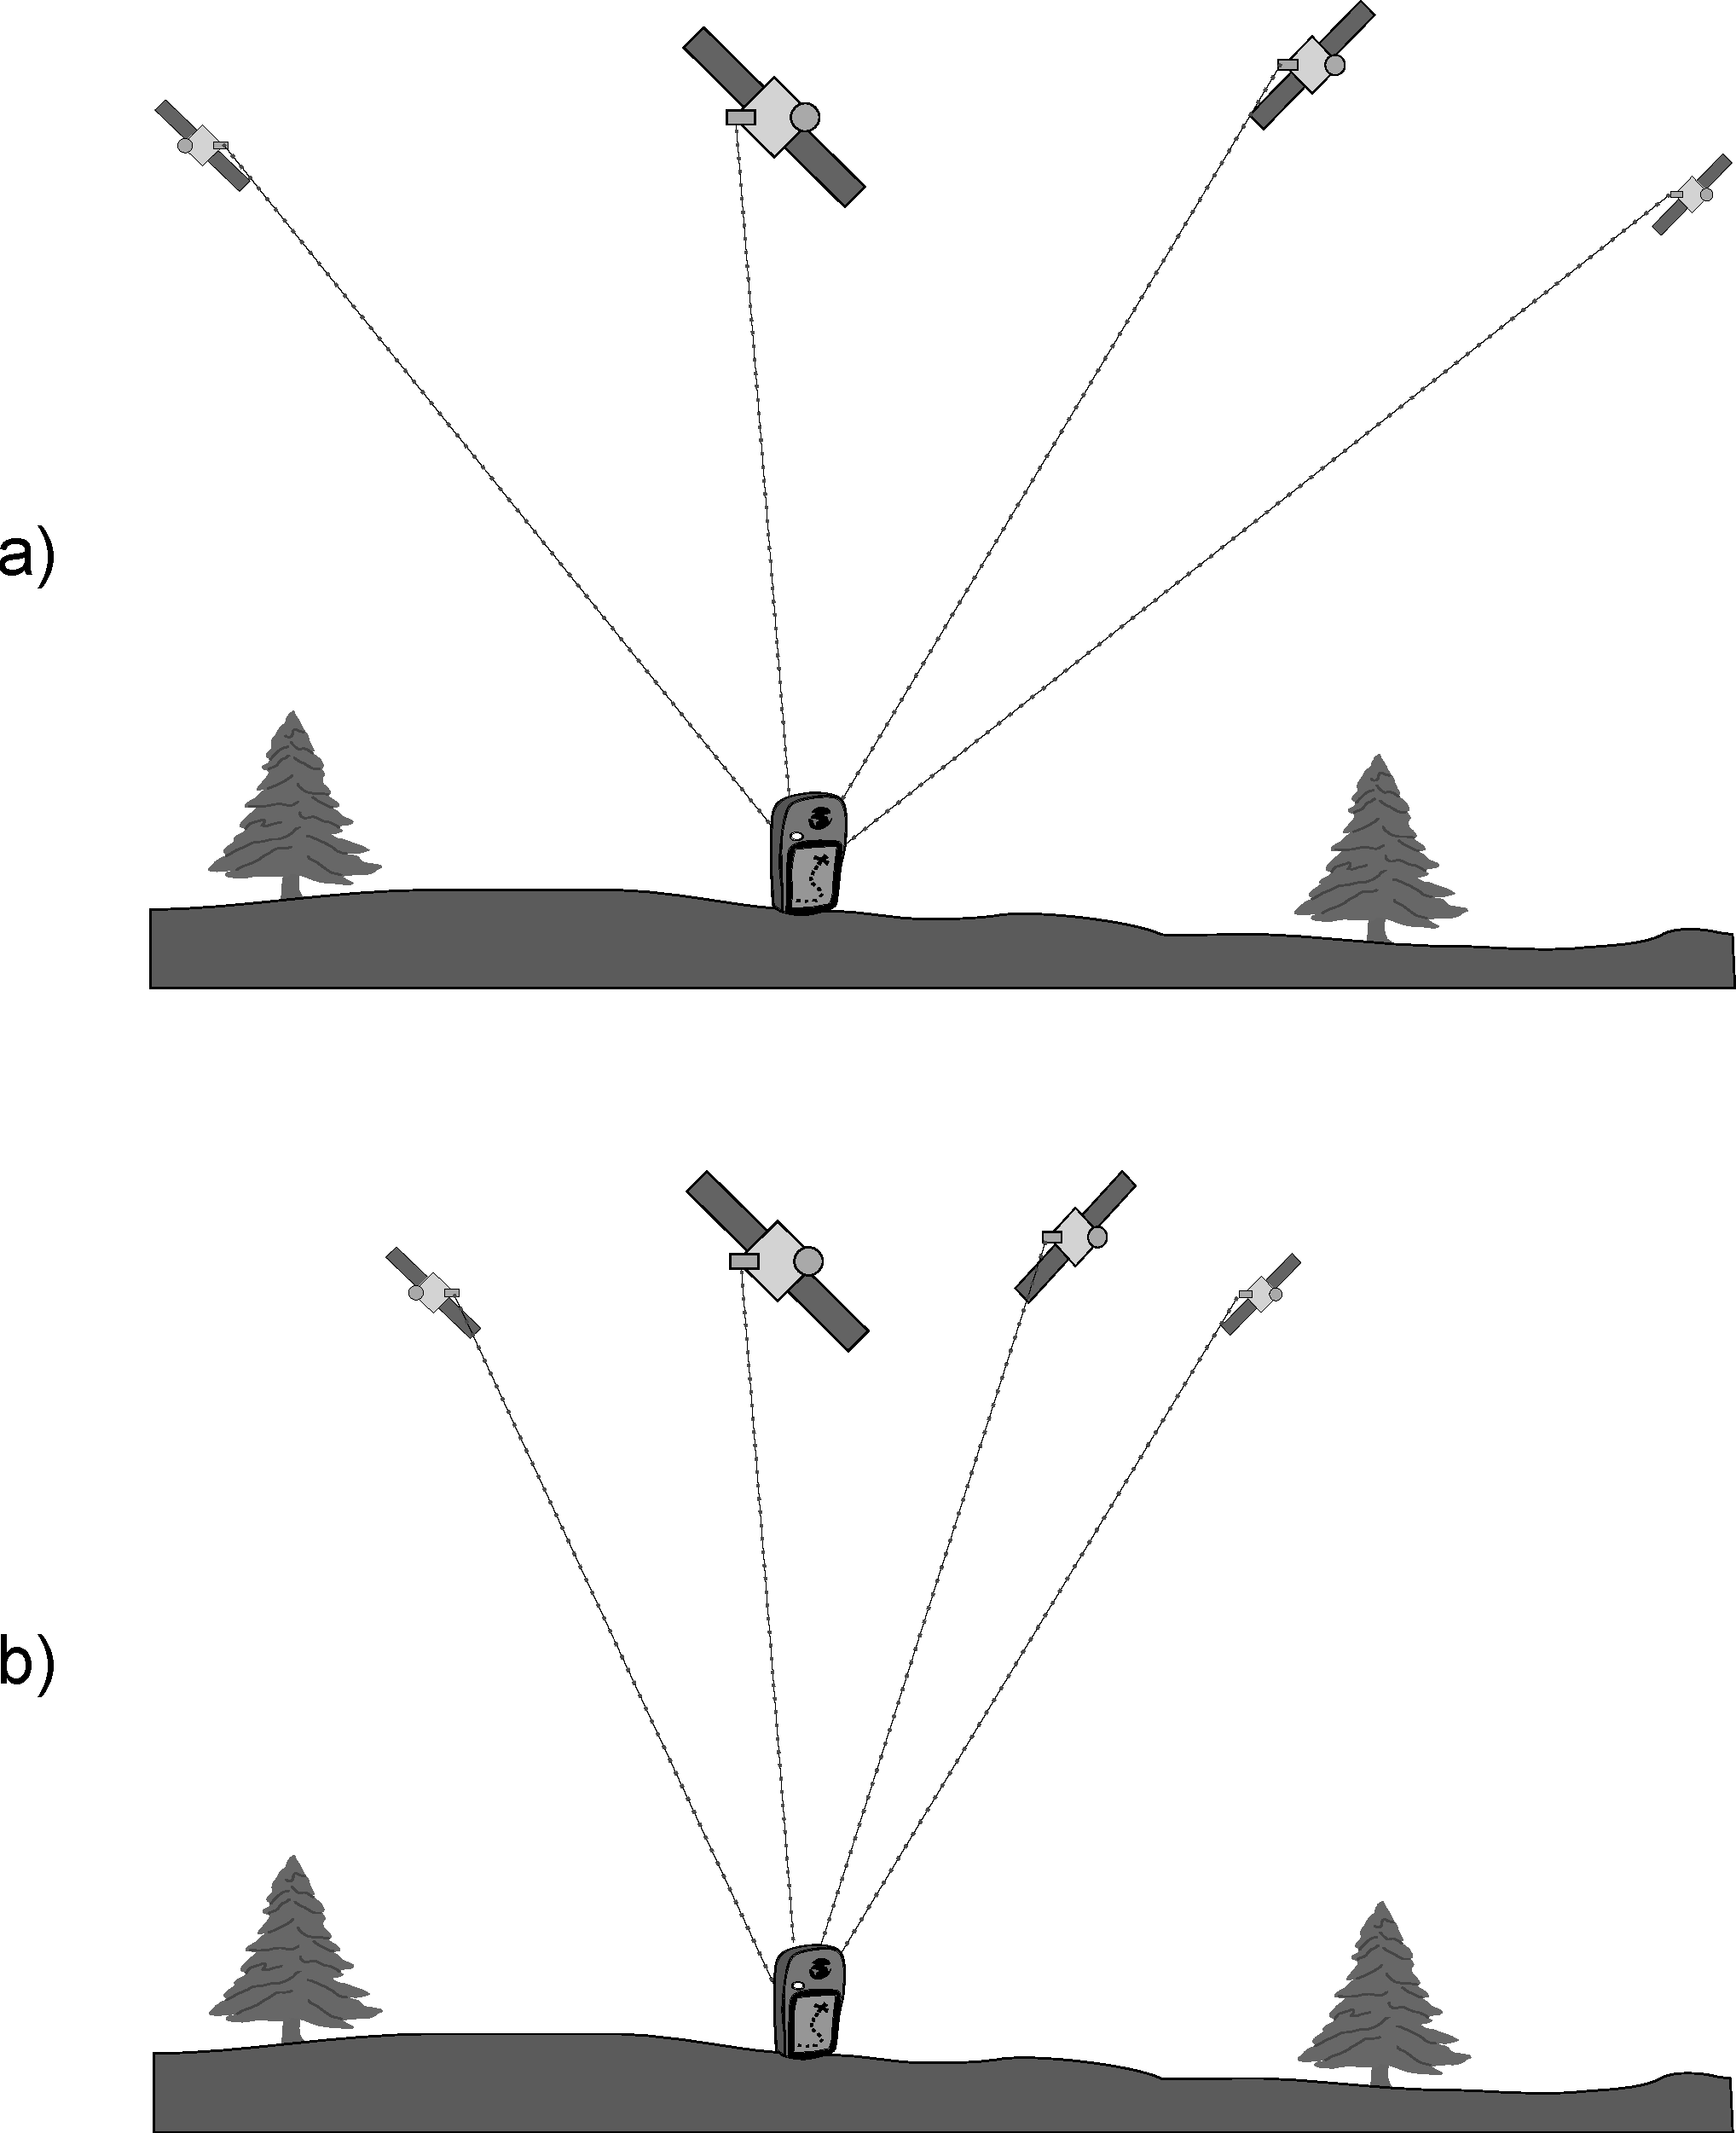
\includegraphics[width=.5\textwidth]{Fuentes_datos/DOP.pdf}
\caption{\small Diluci�n de la precisi�n. La geometr�a de los sat�lites en el ejemplo a) da una mayor precisi�n en el c�lculo de la posici�n del receptor que la del ejemplo b).}
\label{Fig:DOP} 
\end{figure}

Junto a esto, existen otras muchas fuentes de error en el sistema GPS, cada una de las cuales afecta a la precisi�n del mismo. Entre ellas, cabe destacar las siguientes:

\begin{itemize}
	\item Errores en la posici�n de los sat�lites.
	\item Errores por el rebote de la se�al en otros elementos tales como edificios, con anterioridad a alcanzar el receptor.
	\item Errores derivados del paso de la se�al por la atm�sfera. Al atravesar la ionosfera y la troposfera se genera un retraso por la alteraci�n que dicho paso produce sobre la se�al.
	\item Errores en la precisi�n de los relojes, ya mencionados.
	\item \emph{Disponibilidad selectiva}. Debido a su concepci�n como una herramienta militar, el departamento de Defensa de los Estados Unidos, propietario del sistema, introduc�a errores aleatorios en las se�ales, de tal forma que esta quedaba degradada y los usuarios civiles no pod�an obtener una precisi�n muy elevada. La disponibilidad selectiva fue eliminada en el a�o 2000.
\end{itemize}

\index{GPS!fuentes de error}

En conjunto, todos estos errores suman desviaciones apreciables, que sin embargo pueden corregirse con la aplicaci�n de t�cnicas adicionales, por ejemplo incorporando informaci�n adicional procedente de otros receptores. Una de estas t�cnicas es el denominado \emph{GPS diferencial}, pensado en origen para eliminar el error de la disponibilidad selectiva, aunque tambi�n eficaz para corregir una buena parte los restantes errores citados anteriormente.\index{GPS!diferencial}

Para la aplicaci�n del GPS diferencial se requiere no solo un receptor �nico (aquel del cual se quiere calcular su posici�n), sino tambi�n otro receptor fijo de referencia cuyas coordenadas se conocen con alta precisi�n. Este receptor fijo es, a su vez, un receptor de alta precisi�n y, adem�s de calcular su propia posici�n, emite informaci�n que las unidades receptoras pueden aprovechar para corregir sus mediciones. El receptor m�vil, l�gicamente, tiene que soportar este tipo de correcciones, para poder hacer uso de la se�al de la estaci�n de referencia.

Los datos que permiten llevar a cabo la correcci�n puede obtenerse en el receptor mediante radio, descargarse por Internet mediante una conexi�n inal�mbrica, o bien utilizar una constelaci�n de satelites adicional dedicada a elaborar y servir este tipo de datos.

La correcci�n puede realizarse fuera del propio receptor, a posteriori, utilizando software adecuado y los mismos datos de correcci�n que si se realiza la correcci�n en tiempo real.

El fundamento de este sistema es que los errores que afectan al receptor m�vil tambi�n afectan al de referencia. No obstante, la magnitud del error que afecta al receptor de referencia puede conocerse, ya que se conoce la coordenada exacta de este, y en base a eso puede eliminarse el error que afecta al receptor m�vil, asumiendo que ambos errores son de similar �ndole.

En la actualidad, aplicando estas t�cnicas de correcci�n diferencial, un GPS puede obtener precisiones del orden de 2 metros en latitud y longitud, y 3 en altitud\cite{wikipediaGPS}. Sin correcci�n diferencial, esta precisi�n es de unos 10--20 metros.

La figura \ref{Fig:DGPS} muestra un esquema del funcionamiento del GPS diferencial.

\begin{figure}
\centering
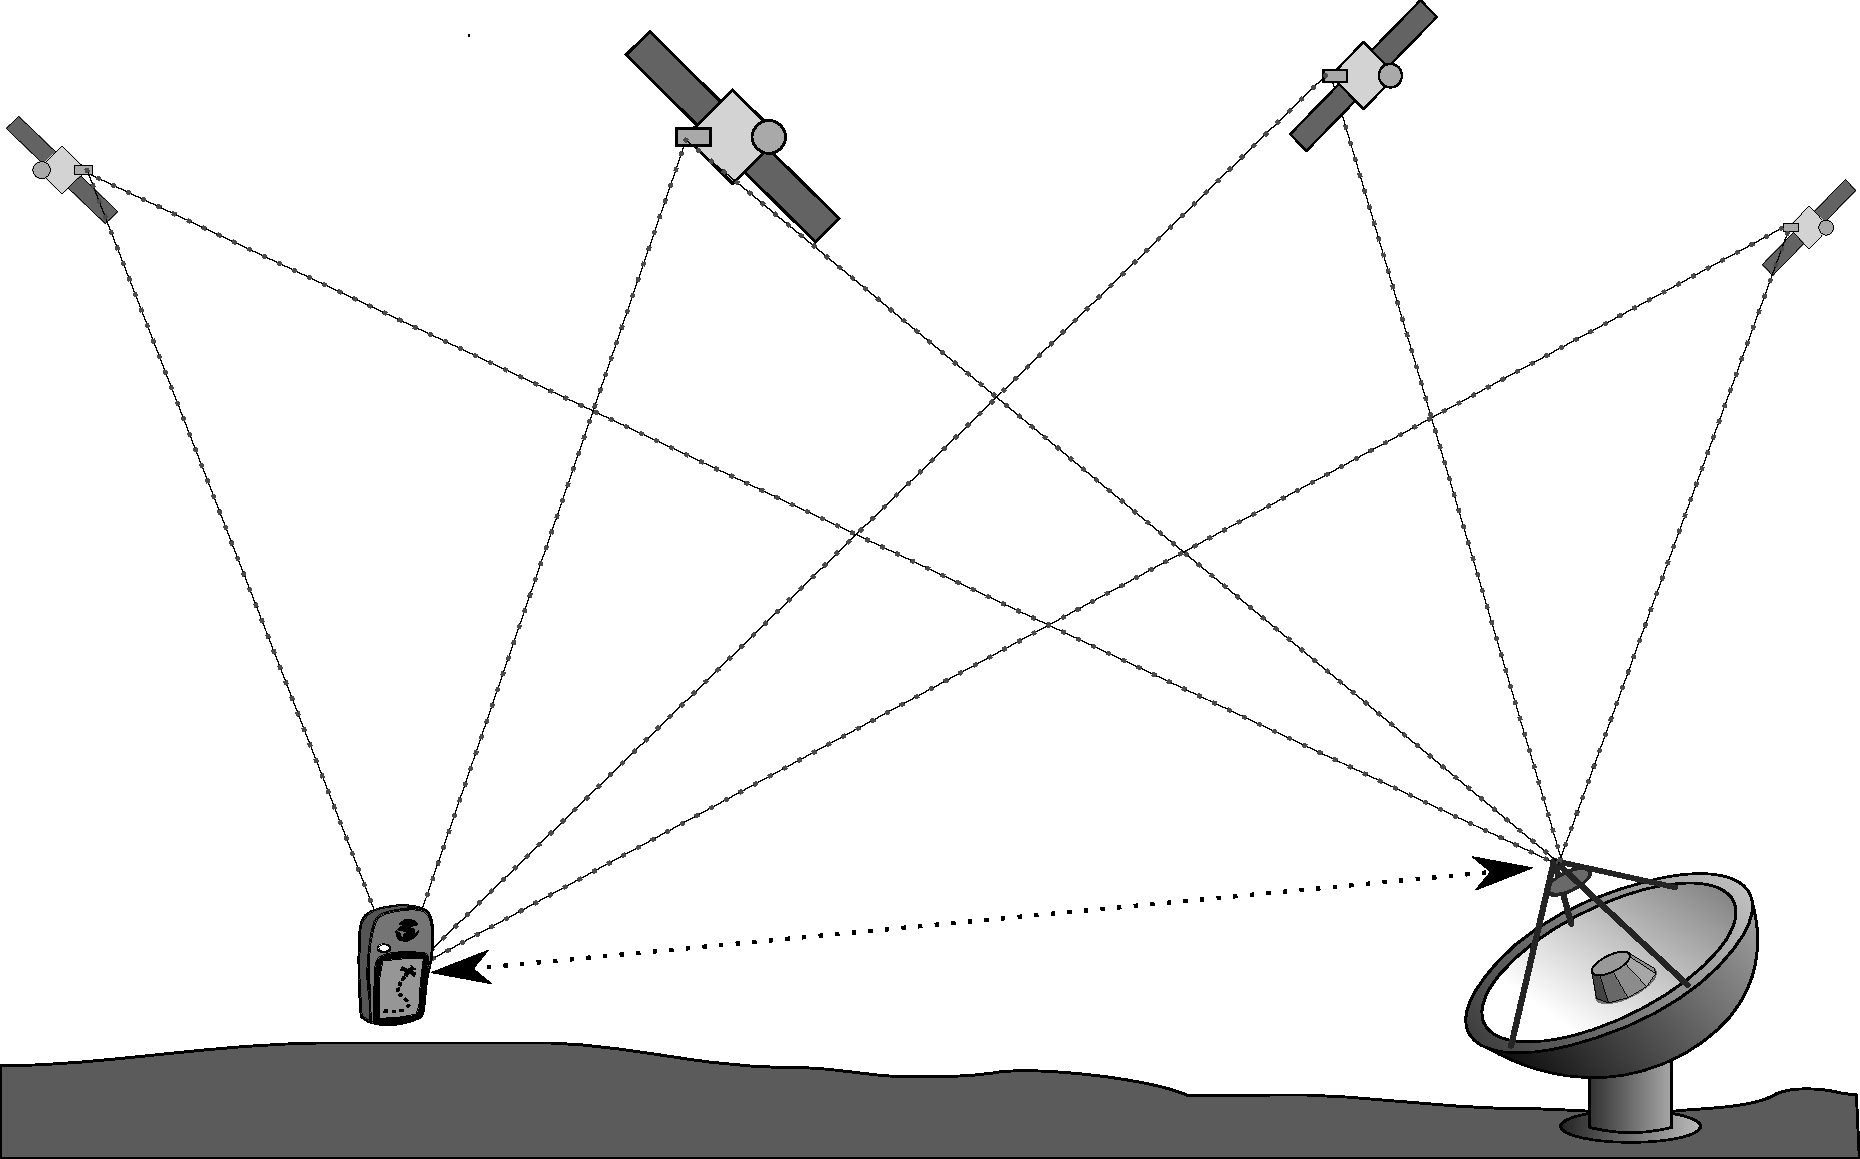
\includegraphics[width=.5\textwidth]{Fuentes_datos/DGPS.pdf}
\caption{\small Esquema de funcionamiento del GPS diferencial}
\label{Fig:DGPS} 
\end{figure}

Adem�s de la literatura abundante sobre GPS, los fabricantes de receptores GPS, muy populares hoy en d�a para numerosas actividades, ponen a disposici�n del p�blico una gran cantidad de informaci�n sobre sus productos y tambi�n sobre los fundamentos del sistema GPS. En ese sentido, una buena referencia es el sitio Web \cite{webTrimble}, donde puede encontrarse una descripci�n detallada de los distintos elementos del sistema GPS, acompa�ada de im�genes y animaciones sumamente did�cticas. En \cite{webHowWorkGPS} tambi�n puede encontrarse informaci�n de inter�s y f�cil acceso.


\subsection{Tipos de receptores}

La precisi�n del sistema global GPS depende del tipo de receptor GPS (o, en el lenguaje com�n, GPS a secas) que se emplee, obteni�ndose mayores precisiones con receptores m�s avanzados, siempre dentro de las posibilidades del propio sistema GPS.

En funci�n de sus caracter�sticas y de la forma en que operan, podemos distinguir los siguientes tipos de receptores GPS:

\begin{itemize}
	\item \textbf{Receptores secuenciales}. Establece conexiones secuenciales con los distintos sat�lites disponibles, estando conectado a uno o dos a lo sumo simult�neamente. Estos receptores son m�s econ�micos, ya que esta forma de operar requiere equipos menos complejos, aunque la precisi�n que se obtiene tambi�n es menor.
	\item \textbf{Receptores continuos}. Disponen de m�s canales de radio que los anteriores y ello permite que la conexi�n a los sat�lites sea continua, sin tener que alternar entre uno y otro. La precisi�n que se obtiene es mayor, pero se trata de equipos m�s caros.
	\item \textbf{Receptores con canales multiplexados}. El esquema de funcionamiento es similar al secuencial, alternando entre los distintos sat�lites y utilizando un �nico canal. No obstante, utilizan software m�s complejo y procesadores m�s potentes, de forma que esta alternancia se puede producir con una frecuencia mucho m�s elevada. 
\end{itemize}

\index{GPS!receptores}

A d�a de hoy, es habitual que incluso los GPS de menor coste tengan m�ltiples canales, permitiendo la conexi�n continua con un n�mero elevado de sat�lites.

Como hemos visto, las se�ales emitidas por los sat�lites contienen dos c�digos (C/A y P) que se transmiten modulados sobre dos ondas portadoras distintas (L1 y L2). No todos los receptores GPS son capaces de utilizar estos elementos de las se�ales, y en funci�n de ello podemos tambi�n clasificarlos. 

Los m�s sencillos �nicamente basan sus c�lculos en el c�digo C/A, mientras que los m�s avanzados y complejos son capaces de utilizar el c�digo P (encriptado, por lo que es necesaria una clave correspondiente), as� como las portadoras para un c�lculo m�s preciso, seg�n se explic� en un punto anterior.

Por �ltimo, y teniendo en cuenta que el sistema GPS mide las coordenadas $(x,y,z)$ y el tiempo, y que existen diferentes precisiones en funci�n de la tecnolog�a que los receptores utilicen, encontramos una gran variedad de unidades receptoras, seg�n estas se adapten para uno u otro uso principal. En l�neas muy generales, los siguientes son algunos de los tipos principales en funci�n de dicho uso.

\begin{itemize}
	\item GPS para uso general. Unidades peque�as y port�tiles, de bajo coste, para actividades al aire libre, donde no se requiere una precisi�n elevada sino simplemente un conocimiento de la posici�n aproximada. Se emplean, por ejemplo, para recoger rutas en senderismo o navegaci�n. Estas unidades, adem�s de informar de la posici�n y ser capaces de almacenar esta, suelen disponer de capacidades de representaci�n de mapas en pantalla, de forma que la informaci�n sobre la posici�n sea m�s �til para el usuario. Otros, como los navegadores GPS para coche, son capaces de calcular rutas �ptimas, combinando la posici�n calculada con una cartograf�a de v�as previamente incorporada al dispositivo.
		La figura \ref{Fig:gps_1}a muestra un receptor GPS de uso general.
	\item GPS para la medici�n topogr�fica. Unidades de medio tama�o, generalmente con una antena independiente que se conecta a la unidad y que el propio operario carga a la espalda. La antena garantiza mayor precisi�n y una mejor localizaci�n de sat�lites en condiciones tales como zonas bajo arbolado. Est�n pensados para un uso profesional en levantamientos o replanteos, ofreciendo buena precisi�n en todas las coordenadas. 
	En la figura \ref{Fig:gps_1}b puede verse unos de estos receptores.
	Estos son los GPS de mayor inter�s para el uso dentro de un SIG, ya que ofrecen datos de campo precisos que cumplen con las necesidades que habitualmente se tienen en un proyecto SIG. Los datos recogidos por estas unidades pueden ser sencillamente incorporados a un ordenador, y en ocasiones la propia unidad dispone de aplicaciones propias, m�s all� de la mera visualizaci�n de cartograf�a asociada, como en el caso anterior.
	\item GPS para la medici�n del tiempo. Estos GPS no resultan de tanto inter�s para su uso en un SIG, ya que se encuentran fijos en un punto y no conceden importancia a la localizaci�n espacial, sino tan solo al tiempo. Se utilizan en estudios que requieran una medici�n muy precisa del tiempo, ya que la referencia temporal que ofrece el sistema GPS es muy precisa y estable.
\end{itemize}

\begin{figure}
\centering
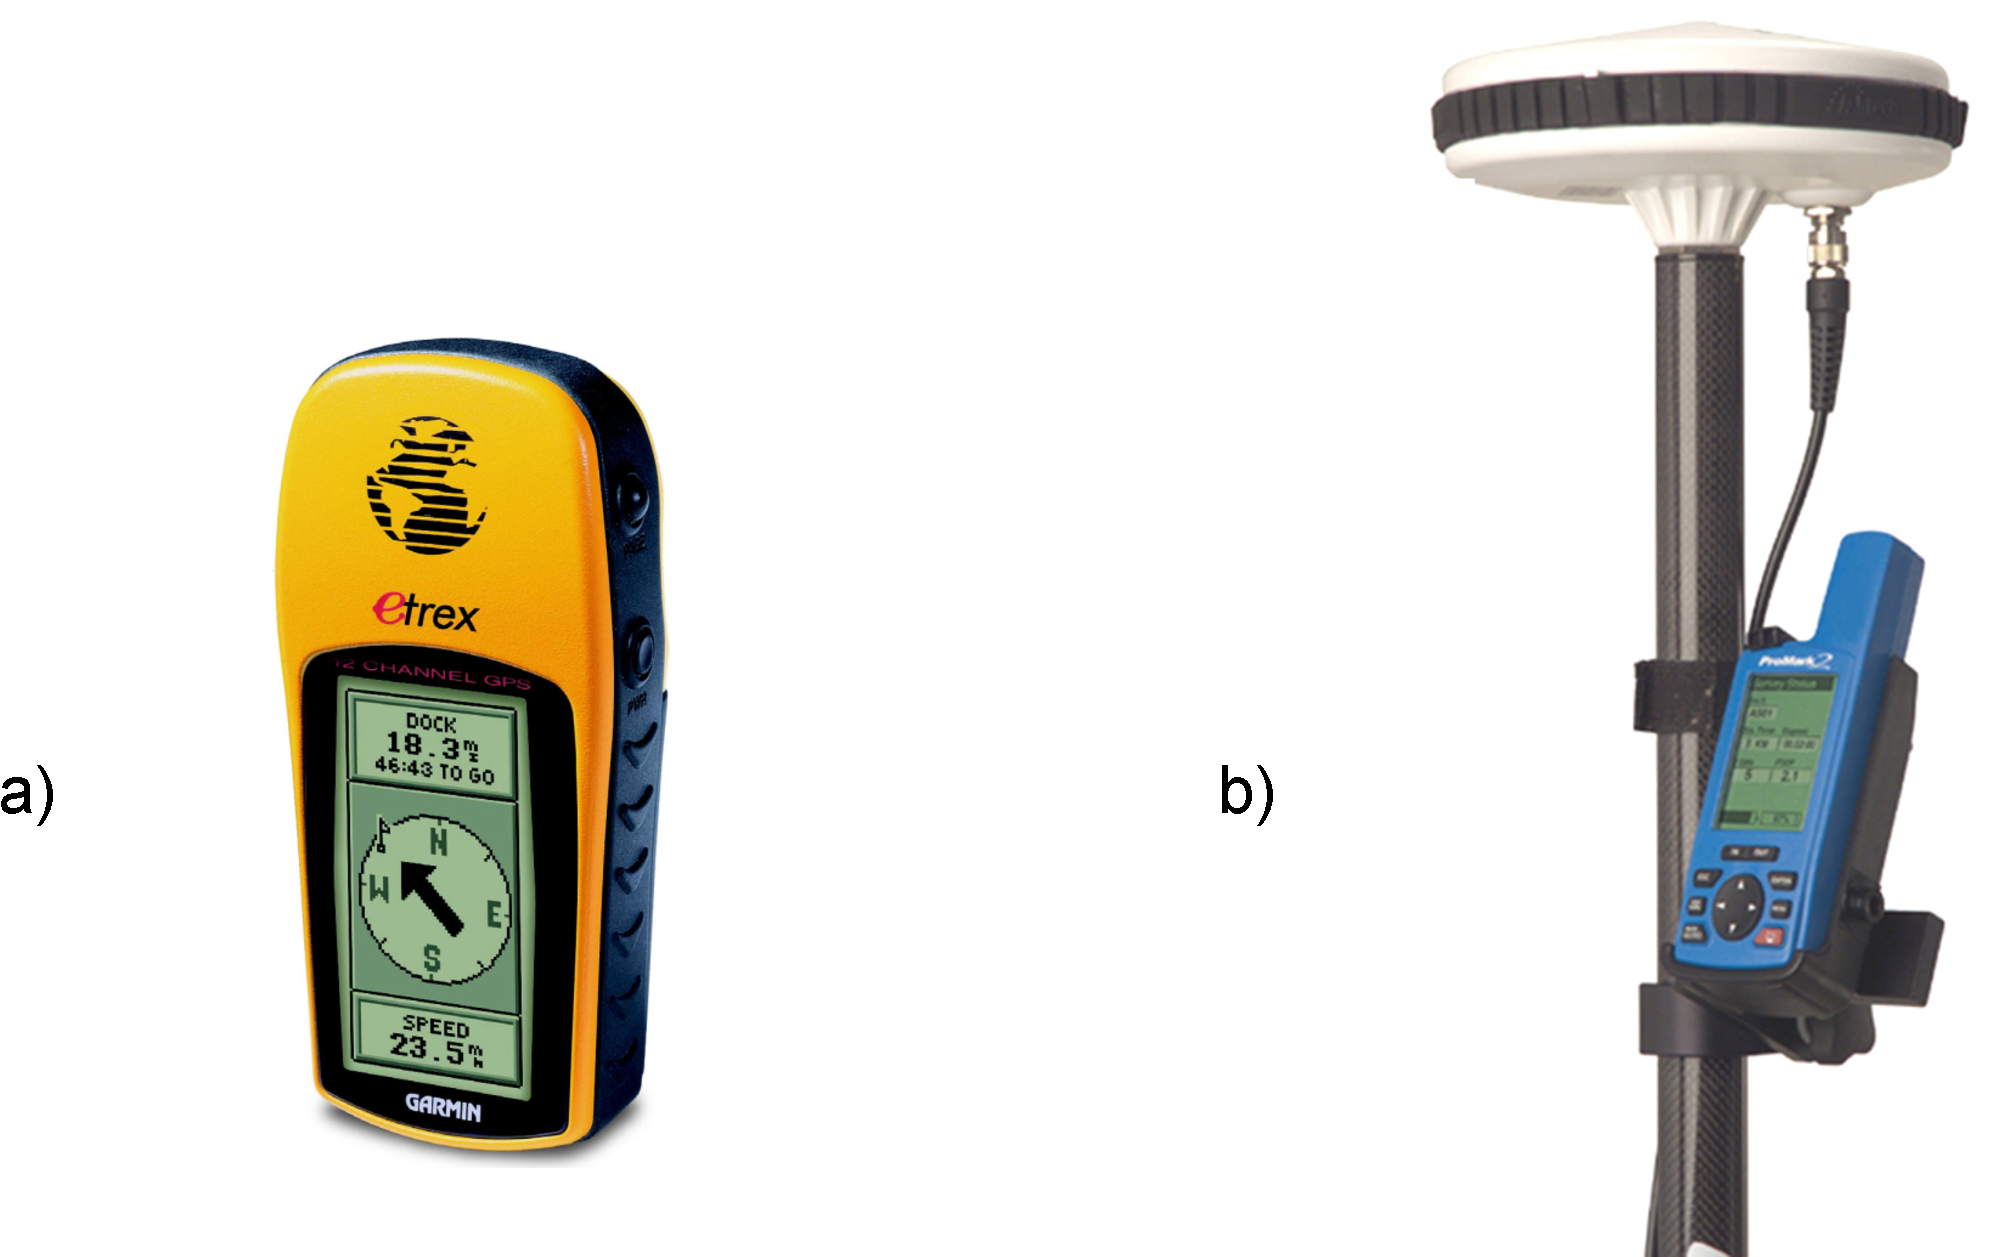
\includegraphics[width=.6\mycolumnwidth]{Fuentes_datos/gps.pdf}
\caption{\small Receptor GPS de bajo coste para uso general (a) y receptor GPS de alta precisi�n con antena externa (b)}
\label{Fig:gps_1} 
\end{figure}

\subsection{Operaciones con la unidad GPS}

La forma en que utilizamos el receptor GPS para recoger los datos que emplearemos posteriormente en el SIG puede ser muy variada en funci�n del tipo de dato, la precisi�n necesaria o las caracter�sticas del propio receptor. 

Los receptores de menor coste est�n generalmente pensados para ser de utilidad directamente en el campo, por ejemplo para localizar un punto concreto y conocer la direcci�n en la que hay que moverse para llegar hasta �l, pero tienen tambi�n capacidad para recoger coordenadas. Estas capacidades son las que resultan de inter�s desde el punto de vista de un SIG, ya que las coordenadas recogidas ser�n despu�s los datos que llevemos a este.

Por su parte, las unidades de mayor precisi�n est�n concebidas para tareas tales como levantamientos topogr�ficos, donde la toma de datos es lo fundamental, pero tambi�n para otras tales como replanteos, donde se requiere situar un punto de coordenadas conocidas. Al igual que en el anterior, las actividades que pueden llevarse a cabo con estos GPS y que interesan desde el punto de vista del SIG son aquellas que van a recoger coordenadas, pues son las que generan datos y convierten al GPS en una fuente de ellos.

Las capacidades de recogida de datos en una unidad GPS de bajo coste permiten almacenar puntos o trazados completos, encontr�ndose el operario inm�vil o bien en movimiento a lo largo de dicho trazado. Es habitual utilizar los vocablos ingleses de la terminolog�a GPS para denotar los distintos elementos que pueden recogerse, conoci�ndose a un punto de inter�s aislado como \emph{waypoint} y un trazado como \emph{track}. Una serie ordenada de \emph{waypoints} se conoce como \emph{route} (ruta).\index{Waypoint}\index{Track}\index{Route}

En el trabajo con el receptor GPS, el operario se puede detener en un punto cualquiera y memorizar las coordenadas del mismo, a�adiendo as� un \emph{waypoint} a la lista de los ya almacenados. Para crear un trazado, se suele disponer de funcionalidades de recogida autom�tica de puntos, de tal modo que el receptor memoriza estos a intervalos fijos de tiempo. El operario simplemente ha de desplazarse por el trazado y dejar que el receptor haga su trabajo mientras tanto. Dependiendo del tipo de dato que quiera obtenerse, la edici�n posterior en gabinete habr� de ser m�s o menos intensa. 

Esta edici�n no est� relacionada solo con la introducci�n de correcciones, sino con la interpretaci�n de los distintos puntos recogidos. Por ejemplo, para registrar el trazado de una calle, el operario puede recorrerla, pero es probable que no lo haga de forma perfectamente rectil�nea. El trabajo posterior con el conjunto de puntos debe resultar en la obtenci�n de una l�nea recta a partir de estos, y ello requiere la interpretaci�n de los datos disponibles.

Pese a que la precisi�n de estas unidades es limitada y no permiten t�cnicas avanzadas de correcci�n (tal precisi�n no es necesarias para las actividades tales como senderismo o navegaci�n para las que han sido dise�ados estos receptores), los GPS de uso cotidiano pueden ser una fuente de datos de primer orden para la recogida de datos. Un ejemplo significativo de ello es el proyecto OpenStreetMap\cite{webOSM}, un proyecto colaborativo para crear mapas libres  cuya principal fuente de datos son unidades GPS sencillas.\index{OpenStreetMap} Este proyecto es uno de los muchos que existen actualmente de este tipo, los cuales se engloban dentro de la idea de \emph{Informaci�n Geogr�fica Voluntaria o Participativa}, sobre la que hablaremos algo m�s adelante en el apartado \ref{VGI}.

Para trabajos de mayor precisi�n tales como levantamientos topogr�ficos, estos receptores no son, sin embargo, suficientes. El uso de receptores m�s precisos y de t�cnicas avanzadas es necesario para obtener precisiones mayores, que pueden ser incluso milim�tricas. 

Estos receptores pueden emplearse individualmente del mismo modo que se hace con un GPS de bajo coste, y registrar puntos de forma similar. La verdadera potencia, no obstante, se obtiene cuando se realizan mediciones con la ayuda de una o varias unidades adicionales, las cuales aportan valores de referencia que permiten aumentar la precisi�n. 

Entre el receptor m�vil y el de referencia se establece una \emph{l�nea base}, y en el c�lculo de la posici�n lo que se calcula es el vector $(x, y, z)$ que une a ambas. Se trata pues, de una medici�n relativa, ya que expresa la posici�n del receptor m�vil a partir de la del receptor de referencia. Puesto que la posici�n de este �ltimo se conoce con gran precisi�n y ese vector tambi�n se calcula con precisi�n, la posici�n buscada que se obtiene es altamente precisa.

La principal ventaja con respecto a m�todos topogr�ficos cl�sicos es que no es necesario que haya visibilidad entre los dos receptores. De esta forma, puede utilizarse una estaci�n de referencia aunque no sea visible desde un punto cuyas coordenadas queremos medir, y las l�neas base pueden ser de mayor longitud.

Otras ventajas tambi�n destacables son el hecho de que puede obtenerse una productividad mucho mayor, ya que una �nica unidad de referencia puede ser utilizada por varias unidades m�viles.

El n�mero de t�cnicas existentes en la actualidad para realizar este tipo de mediciones (ya sea con uno o con varios receptores) es variada. El hecho de que se busquen mediciones precisas hace que se realicen mediciones utilizando la fase de la portadora, que como vimos implica una mayor necesidad de tiempo para registrar correctamente una posici�n. En funci�n de las caracter�sticas de la linea base y los requerimientos concretos del trabajo, ser�n unas u otras las m�s adecuadas para cada caso. 

La diferencia principal entre estas t�cnicas es el tiempo necesario para la recogida de un punto. En general, un mayor tiempo equivale a una mayor precisi�n. Entre las t�cnicas habituales, cabe citar las siguientes:

\begin{itemize}
	\item \textbf{Est�tico}. En base a dos puntos de referencia (con una unidad GPS fija en cada uno de ellos), se calcula la posici�n de un tercero en un punto dado. Se trata del m�todo m�s preciso, pero requiere tiempos de observaci�n muy largos (superiores a una hora), lo que lo hace inadecuado para levantamientos o replanteos. Este tipo de procedimientos se emplean casi exclusivamente en trabajos geod�sicos y las lineas base pueden ser de gran longitud. 
	\item \textbf{Est�tico r�pido}. Igual que el anterior, pero con tiempos menores, del orden de 5--10 minutos por punto medido.	
	\item \textbf{Cinem�tico}. En el m�todo cinem�tico los tiempos son a�n menores que en el est�tico r�pido, del orden del minuto. El fundamento de la t�cnica es distinto a los anteriores, ya que tras la inicializaci�n el receptor m�vil puede desplazarse con m�s velocidad y no es necesario que se detenga durante un periodo largo de tiempo en cada punto, pero ello exige que durante el desplazamiento tanto la unidad m�vil como la fija de referencia mantengan la recepci�n de las se�ales, que han de ser de al menos cuatro sat�lites (preferiblemente cinco), y los mismos para ambas unidades. Si alguna de ellas pierde la conexi�n, se hace necesario repetir de nuevo el proceso de inicializaci�n \cite{Remondi1988IN}.
	
	Existe una gran variedad de procedimientos de tipo cinem�tico, cuya filosof�a es esencialmente la misma, pero bajo nombres distintos. Aunque pueden existir diferencias en los fundamentos te�ricos, la forma de proceder es en muchos casos muy similar. T�cnicas como \emph{Stop \& Go}\index{Stop \& Go} o \emph{pseudocinem�tico} pueden incluirse en este tipo de m�todos. En general, estos y otros se engloban bajo la denominaci�n de procedimientos cinem�ticos, aunque sus caracter�sticas sean distintas en cada caso. 
	
	Muchos de estos procedimientos vienen definidos por el equipo a utilizar, y los tiempos de paradas en cada punto medido, as� como otros aspectos, son recomendados por el propio fabricante. La forma m�s correcta de llevar a cabo una toma de datos en campo, en este caso, es seguir las indicaciones concretas del fabricante de para cada producto.
	
	Un caso particular dentro de los m�todos cinem�ticos es el \emph{cinem�tico en tiempo real} (RTK)\footnote{Real Time Kinematic}, en el que, a diferencia de los anteriores, las correcciones necesarias se efect�an en tiempo real y no requieren postproceso. Se trata de la t�cnica m�s actual, y proporciona al operario mediciones exactas de su posici�n de forma instant�nea, con las ventajas que ello conlleva. Las mediciones son m�s precisas, ya que el operario que las toma conoce el valor recogido en el mismo momento de hacer la medici�n, y puede de esa forma realizar una comprobaci�n en el acto. Informaci�n m�s detallada sobre esta t�cnica puede encontrarse en \cite{Rizos1998BCG}.
\end{itemize}\index{Real Time Kinematic}

Para profundizar m�s al respecto, en \cite{Asenjo1997UPV} puede encontrarse informaci�n sobre la realizaci�n de levantamientos con GPS, as� como en \cite{GPSUSArmy}.

En base a los ejemplos anteriores, y para concluir esta parte, podemos dar una clasificaci�n de las operaciones con un receptor GPS en funci�n de tres criterios b�sicos: el n�mero de unidades que se emplean simult�neamente, el movimiento (o ausencia de �l) del receptor y el momento en el que se obtiene el dato ya listo para su utilizaci�n posterior.

Seg�n el n�mero de unidades, tenemos:

\begin{itemize}
	\item \textbf{Absolutas}. Se tiene un �nico receptor y un �nico operario. La posici�n se calcula con la informaci�n de los sat�lites, sin apoyo de otra unidad adicional.
	\item \textbf{Relativas}. Se emplea una unidad adicional a modo de referencia. Las medidas se basan en la informaci�n de los sat�lites y la que aporta dicha unidad de referencia, y la posici�n se calcula en relaci�n a esta en lugar de en t�rminos absolutos. Estas operaciones alcanzan un grado de precisi�n mayor que las de tipo absoluto.
\end{itemize}

Atendiendo al movimiento del receptor encontramos:

\begin{itemize}
	\item \textbf{Est�ticas}.
	\item \textbf{Cinem�ticas}.
	\item \textbf{Variantes intermedias}.
\end{itemize}

Por �ltimo, en funci�n de la obtenci�n de datos, distinguimos:

\begin{itemize}
	\item \textbf{En tiempo real}. Las correcciones pertinentes se realizan en el acto, y el resultado que se visualiza en el receptor o se almacena en este ya ha sido filtrado y corregido.
	\item \textbf{Con necesidad de postproceso}. Las correcciones se realizan en gabinete posteriormente, con informaci�n que el receptor no posee o no es capaz de procesar de modo inmediato durante su utilizaci�n.
\end{itemize}

\subsection{Integraci�n de GPS y SIG}

\index{GPS!integraci�n con SIG}

La utilidad de un GPS como fuente de datos para el trabajo en un SIG es innegable. Multitud de trabajos que requieren la toma de datos en campo y la medici�n de coordenadas pueden efectuarse ventajosamente con equipos GPS, y la informaci�n derivada de ese uso puede ser posteriormente incorporada a un SIG.

EL GPS puede emplearse como una fuente de datos est�tica (se utiliza como herramienta para la creaci�n de una capa de informaci�n geogr�fica y esta despu�s se emplea en el SIG de la forma habitual), o bien para la obtenci�n de datos en tiempo real. Los SIG sobre dispositivos m�viles (v�ase el apartado \ref{SIG_Moviles}) pueden aprovechar los receptores GPS que estos dispositivos habitualmente incorporan, y alimentarse con los datos de dichos receptores en tiempo real.

Un caso particular de esto son los cada d�a m�s populares navegadores GPS. Estos dispositivos aunan el receptor GPS y una aplicaci�n de tipo SIG que presenta un visor y permite ejecutar un n�mero reducido de procesos, en concreto los de c�lculo de rutas �ptimas entre dos puntos a trav�s de una red de comunicaci�n (apartado \ref{Rutas_optimas}). Uno de los puntos (el de destino) es fijado por el usuario, mientras que el punto de origen es el punto actual en que se encuentra el dispositivo, que se obtiene a partir del GPS.

Como herramientas est�ticas, el trabajo en campo con un GPS genera un conjunto de puntos o de trazados, que pueden f�cilmente transferirse al ordenador para poder trabajar con ellos. Este trabajo puede realizarse dentro de un SIG, ya que, o bien este incluye la capacidad de importar los archivos generados por el GPS, o el software que acompa�a a dicho GPS incorpora herramientas para ayudar en la comunicaci�n entre SIG y GPS.

Adem�s de la informaci�n posicional que deriva del sistema GPS, los receptores GPS pueden incorporar elementos que permitan la entrada de la componente tem�tica asociada a las distintas entidades, es decir, los atributos. Si solo se registra la componente espacial, la informaci�n que se almacena en el GPS es de mucha menos utilidad que si se acompa�a de atributos.

Las funcionalidades incorporadas en el receptor suelen ser sencillas, pero permiten que desde este se pueda llevar a cabo todo el proceso de creaci�n de la capa que posteriormente se emplear� en el SIG. El trabajo de campo incluye de este modo tanto el registro y creaci�n de las entidades como la edici�n de las propiedades no espaciales de estos. Existe, no obstante, la posibilidad de completar la fase de introducci�n de atributos en el SIG, durante el trabajo en gabinete, lo cual en ocasiones resulta m�s sencillo y pr�ctico.

El volumen de trabajo que se requiere una vez que los datos han sido recogidos depender� tambi�n de las necesidades de precisi�n que se presenten y del tipo de trabajo en que se enmarque dicha recogida de datos. La realizaci�n de correcciones y la edici�n avanzada de los datos no puede en ocasiones realizarse dentro de un SIG, ya que este no dispone de las herramientas necesarias para un tratamiento avanzado de los datos del GPS. El SIG est� preparado para trabajar con las coordenadas que salen del GPS, pero este puede almacenar m�s datos (datos <<en bruto>>), que pueden procesarse en gabinete para la obtenci�n de dichas coordenadas de forma m�s precisa. Para realizar esta tarea  es necesario software especializado, y las funcionalidades del SIG se emplear�n posteriormente, cuando ya se hayan verificado los datos del GPS y elaborado las capas correspondientes.

Para el lector interesado, una referencia completa sobre el uso de GPS de cara a la integraci�n de los datos en un SIG es \cite{Steede2000ESRI}.  En el ya mencionado apartado \ref{SIG_Moviles} veremos con detalle la tecnolog�a de los SIG m�viles, un �mbito en el que SIG y GPS se unen para conformar herramientas conjuntas. 

\section{Informaci�n Geogr�fica Voluntaria}
\label{VGI}

Hemos mencionado ya que los dispositivos tales como receptores GPS de bajo coste pueden emplearse para recoger informaci�n geogr�fica y crear datos geogr�ficos, y que cuando esto se une a los conceptos participativos de la denominada Web 2.0, surgen iniciativas de gran inter�s en las que el usuario de a pie, sin necesidad de una formaci�n espec�fica como cart�grafo, puede aportar sus datos para que otros los exploten posteriormente. Aunque no se trata de una fuente de datos como tal, y los elementos y dispositivos empleados ya los hemos visto a lo largo de este cap�tulo, el cambio que supone la inclusi�n de una filosof�a acorde con las ideas de la Web 2.0 es tan notable que merece ser tratado por separado. No se trata de un cambio en la propia toma o preparaci�n de datos, o de una tecnolog�a nueva que se aplique a estos, sino de un cambio social y filos�fico que redefine el propio concepto de la informaci�n geogr�fica en lo que a la creaci�n del dato geogr�fico respecta, y cuyas consecuencias son ciertamente importantes, ya que abren el �mbito de la creaci�n cartogr�fica a un nuevo y amplio grupo de personas.\index{Web 2.0}

Se conoce como \emph{Informaci�n Geogr�fica Voluntaria o Participativa} (en ingl�s Volunteered Geographical Information, VGI)\cite{Goodchild2007VGI} al uso de Internet para crear, gestionar y difundir informaci�n geogr�fica aportada voluntariamente por usuarios de la propia red. El conjunto de herramientas y t�cnicas que emplean esos usuarios para aportar su informaci�n conforma lo que se ha dado en llamar \emph{neogeograf�a}. La comparaci�n entre proyectos de creaci�n de VGI y la bien conocida Wikipedia, tal y como se coment� en otro punto anterior en este mismo cap�tulo, sirve perfectamente para ilustrar qu� es lo que entendemos por VGI y neogeograf�a.
\index{Neogeograf�a}\index{VGI}\index{Informaci�n Geogr�fica Voluntaria|see{VGI}}\index{Wikipedia}

En el caso particular de esta �ltima, la neogeograf�a ha supuesto un profundo cambio en algunas de las ideas b�sicas de la cartograf�a, modificando asimismo la concepci�n tradicional de la informaci�n geogr�fica, sus caracter�sticas o el papel que esta ven�a desempe�ando en muchos �mbitos (o incluso d�ndole un papel en campos donde con anterioridad el uso de informaci�n geogr�fica era escaso). Algunas de las ideas principales sobre la neogeograf�a son las siguientes:

\begin{itemize}
	\item Popularizaci�n y democratizaci�n. La producci�n cartogr�fica ha estado siempre en manos de gobiernos u organismos, y en muchas ocasiones fuertemente censurada debido a su elevado valor estrat�gico. Con la VGI, la creaci�n de informaci�n geogr�fica se democratiza y se convierte en un proceso participativo libre y sin restricciones.  Se invierte el esquema <<hacia abajo>> de producci�n y uso de informaci�n geogr�fica.
	\item Los ciudadanos se convierten en <<sensores>> y tienen mayor consciencia de su realidad geo--espacial.
	\item Se elimina parte del <<misticismo>> de la producci�n de informaci�n geogr�fica	
\end{itemize}

En parte, estas ideas son tambi�n comunes a otros fen�menos basados en la Web 2.0, ya que todas se fundamentan en una mayor democratizaci�n de la informaci�n, sea esta geogr�fica o no. Tambi�n se comparten algunos de los problemas o cr�ticas que otros �mbitos han recibido al adoptar esquemas de producci�n similares. Por ejemplo, la calidad de la informaci�n es puesta en entredicho al promover la participaci�n de todo tipo de personas, con independencia de su perfil. En el caso de la informaci�n geogr�fica, con una producci�n tradicionalmente como hemos dicho limitada a profesionales muy especializados, esto es especialmente relevante. Con la proliferaci�n de la VGI, se da voz y poder sobre la informaci�n geogr�fica a individuos en gran medida sin formaci�n, que no obtienen un beneficio tangible obvio y no pueden aportar garant�as de veracidad o autoridad alguna. Esto puede plantear dudas l�gicas acerca de la conveniencia de usar esa informaci�n.

No debe olvidarse no obstante, que la Web 2.0 tambi�n tiene sus mecanismos de regulaci�n, y que en otros casos ya se ha demostrado que, para otros tipos de informaci�n, la calidad y rigor de esta no es inferior a la creada con esquemas m�s cl�sicos y menos abiertos. Un hecho particularmente curioso que tiene lugar a este respecto con la informaci�n geogr�fica es el relacionado con los denominados \emph{elementos trampa}, y particularmente con el m�s popular de ellos, las \emph{calles trampa}. Aunque se trata de una pr�ctica negada por buena parte de los productores de cartograf�a, es sabido que estos introducen elementos err�neos (tales como una calle inexistente en un callejero) como medida para proteger sus derechos de autor y poder reconocer copias ilegales. En el caso de la VGI, puesto que no existe esa necesidad ya que la informaci�n generada y aportada por los voluntarios es libre, no existen este tipo de errores intencionados. La comparaci�n de informaci�n geogr�fica cl�sica con VGI ha puesto de manifiesto que se trata de una pr�ctica real que, obviamente, disminuye la calidad del dato geogr�fico.

Por otra parte, el hecho de que se use equipo de bajo coste y los usuarios no sean t�cnicos especializados no es necesariamente un problema. Un usuario sin formaci�n no est� capacitado para efectuar un levantamiento topogr�fico preciso, pero s� para situarse delante de la puerta de una tienda y marcar su posici�n, a�adiendo esta a un proyecto que catalogue los comercios de la zona y su localizaci�n. Este tipo de informaci�n geogr�fica, de puntos de inter�s muchas veces no recogidos en cartograf�a m�s especializada, constituye una gran parte de la VGI, y las metodolog�as e instrumental con que se crea son m�s que suficientes para otorgarle validez y precisi�n adecuada al uso del que posteriormente va a ser objeto.

En resumen, la neogeograf�a es en la actualidad un fen�meno que no debe dejarse de lado, ya que los proyectos que aglutina se est�n convirtiendo paulatinamente en proveedores fundamentales de datos cuya calidad en muchos casos es excelente.

Aunque las hemos tratado dentro de este cap�tulo dedicado a las fuentes de datos, la VGI y la neogeograf�a tienen una indudable vinculaci�n con todo lo desarrollado en la parte de este libro dedicada al factor organizativo, ya que se trata de un fen�meno social m�s que t�cnico. De igual modo, el cap�tulo \ref{SIG_movil}, dedicado a los SIG m�viles, est� tambi�n muy relacionado con ambas, puesto que son los dispositivos y aplicaciones que veremos entonces, as� como los servicios sobre ellos, los que han posibilitado el desarrollo de la neogeograf�a y la abundante producci�n actual de VGI. \index{SIG m�vil}


\section{Sobre cartograf�a de elevaciones}

La cartograf�a de elevaciones es probablemente la de mayor importancia de entre todas las que se emplean de forma habitual dentro de cualquier proyecto SIG. Su relevancia deriva del hecho fundamental de que la practica totalidad de procesos que se estudian en un SIG tienen alg�n tipo de componente relacionada con el terreno y su relieve, y por tanto puede obtenerse amplia informaci�n sobre dichos procesos a partir de una capa con datos de elevaci�n.

Como dato relevante, dedicaremos en este libro un cap�tulo entero, el \ref{Geomorfometria}, al conjunto de operaciones de an�lisis basadas en el MDE\index{Modelo Digital de Elevaciones}, que van desde el simple c�lculo de pendientes hasta la extracci�n de par�metros m�s complejos, pasando por la definici�n del comportamiento hidrol�gico de una zona seg�n las caracter�sticas de su relieve, entre otros. Asimismo, gran n�mero de otras formulaciones que veremos en la parte dedicada a procesos tienen su principal aplicaci�n sobre datos de elevaci�n, en particular los m�todos de interpolaci�n que veremos en el cap�tulo \ref{Creacion_capas_raster}, y que nos permitir�n crear cartograf�a de elevaciones en formato r�ster. Este es, como veremos, el formato preferido para el an�lisis de la cartograf�a de elevaciones, ya que ofrece un mayor abanico de posibilidades frente a otros.\index{Interpolaci�n}

Aunque el formato r�ster es el m�s indicado para llevar a cabo los an�lisis correspondientes, la cartograf�a de elevaciones puede crearse originalmente con muy diversas caracter�sticas. De igual modo, y debido tambi�n a la gran importancia de este tipo de capas, su origen puede ser muy variado, ya que son muchas las t�cnicas distintas que existen para su creaci�n. Es de inter�s, por tanto, exponer en este cap�tulo sobre fuentes de datos algunas de las ideas principales relativas a la creaci�n de capas de elevaciones, las caracter�sticas de estas o las ideas fundamentales que residen tras las metodolog�as m�s importantes. Posteriormente, esto nos ayudar� a entender mejor las restantes formulaciones y conceptos relativos al manejo y an�lisis de este tipo de cartograf�a, abundantes en este libro como ya se ha dicho.

A modo de resumen, he aqu� una lista de metodolog�as a partir de las cuales puede obtenerse cartograf�a de elevaciones, gran parte de las cuales han sido tratadas con detalle antes en este mismo cap�tulo.

\begin{itemize}
\item \textbf{GPS}. Como ya sabemos, un GPS toma datos no solo de la posici�n que ocupa en coordenadas $x$ e $y$, sino tambi�n su elevaci�n. La utilizaci�n de GPS permite obtener una nube de puntos de elevaci�n, aunque si esta ha de cubrir un territorio amplio y con cierta precisi�n en las medidas, resulta poco id�neo el trabajar con esta tecnolog�a, ya que es costoso en tiempo. Es m�s adecuada para obtener levantamientos precisos de �reas m�s reducidas, donde se demuestra como una herramienta sumamente eficaz.
\item \textbf{Digitalizaci�n de curvas de nivel}. En ocasiones la cartograf�a de elevaciones ya existe, aunque no en el formato adecuado para su empleo en un SIG. Ya conocemos los m�todos de digitalizaci�n de entidades, tanto manuales como autom�ticos, y ya sea en pantalla o en equipo especializado, y mediante ellos podemos digitalizar las curvas de nivel, obteniendo una capa de l�neas con la informaci�n altitudinal que contiene un mapa topogr�fico habitual.\index{Digitalizaci�n!de curvas de nivel}\index{Curva!de nivel!digitalizaci�n}
\item \textbf{Estereograf�a}. A partir de pares estereosc�picos, y con el concurso de una estaci�n fotogram�trica digital pueden delinearse l�neas o puntos de una elevaci�n dada, digitalizando as� la informaci�n altim�trica. El procedimiento es similar a la simple digitalizaci�n de curvas de nivel, solo que en este caso estas no est�n presentes expl�citamente en las im�genes de partida, y se infieren a partir de la visualizaci�n tridimensional de las mismas.\index{Estereograf�a}
\item \textbf{Interferometr�a}. La interferometr�a es una t�cnica cuyos fundamentos son en cierta medida similares a los de la estereograf�a, pues se basan en la informaci�n recogida de un punto concreto desde dos puntos distintos. Si en el caso de emplear simples im�genes esto permit�a crear una imagen tridimensional, en el caso de la interferometr�a el estudio de las diferencias de fases entre las ondas recibidas en dos puntos distintos permite el c�lculo de distancias. Se trata, por tanto, de un proceso automatizado, que requiere menos intervenci�n que en el caso de la restituci�n fotogram�trica.\index{Interferometr�a}

Un uso muy habitual de esta t�cnica es con los denominados \emph{Radares de Apertura Sint�tica}\footnote{Synthetic Aperture Radar (SAR)}, utilizado por ejemplo en el caso de la misi�n SRTM, que rese�amos anteriormente como producto importante. La medici�n desde dos puntos puede hacerse con dos pasadas de sat�lite (caso por ejemplo del ERS) o bien en una sola si la plataforma dispone de dos receptores separados una cierta distancia (caso del SRTM). En \cite{SARInterferometry} puede encontrarse una descripci�n detallada de este tipo de t�cnicas y las etapas que comprenden.
\item \textbf{LiDAR}. La t�cnica m�s avanzada en la actualidad es el uso de aparatos de altimetr�a basados en l�ser, como el LiDAR, que ya hemos visto en este mismo cap�tulo. El LiDAR ofrece posibilidades muy interesantes tales como la obtenci�n de MDE y MDS (Modelo Digital de Superficie) por separado. \index{Radar de Apertura Sint�tica}\index{Synthetic Aperture Radar}\index{LiDAR}\index{SRTM}\index{Modelo Digital de Superficie}

El resultado de un trabajo con LiDAR es una nube de puntos, normalmente en un n�mero muy elevado debido a la precisi�n del instrumento, la cual puede emplearse para crear otro tipo de capas, tales como capas r�ster. El nivel de postproceso que se requiere para la obtenci�n final de una capa es mucho menor que con otras t�cnicas.
\end{itemize}

A la hora de plantear un proyecto SIG, debe elegirse entre estas fuentes, tanto si se desea adquirir la cartograf�a ya elaborada como si se desea crearla a partir de otras fuentes. La variedad de opciones existentes es grande, y cada una de ellas tiene sus caracter�sticas peculiares. Para saber m�s al respecto, algunas referencias donde puede encontrarse una comparaci�n entre las metodolog�as anteriores son \cite{Nikolakopoulos2006IJRS}, \cite{Mercer1999ISPRS} y \cite{Mercer2001PW}.

\section{Formatos de archivo}
\label{Formatos_archivo}

Como hemos visto, las fuentes de datos son muy variadas, y a la hora de elaborar un proyecto SIG podemos recoger datos de muchas procedencias distintas. Conocer todas estas fuentes de datos es importante para elaborar una base de datos geogr�fica que permita obtener los mejores resultados posibles, pero tambi�n lo es el conocer la forma en que esos datos pueden obtenerse. Los datos geogr�ficos se van a almacenar en archivos, existiendo muchos formatos de archivo distintos para recoger un mismo conjunto de datos.

Estos archivos son la materializaci�n de los modelos de almacenamiento que ve�amos en el apartado \ref{Modelos_almacenamiento}, y su existencia obedece a distintas razones. Pueden haber sido definidos por alguna casa comercial para ser utilizados en su software, por un colectivo, o bien pueden ser est�ndares internacionales definidos para tratar de homogeneizar la forma en que se presentan los datos dentro de un determinado �mbito de trabajo.

Datos de una misma procedencia pueden presentarse de forma distinta si se emplean diferentes formatos de archivo. Las circunstancias por las cuales se opta por uno u otro formato pueden basarse �nicamente en el hecho de que el software empleado soporte o no dicho formato, pero deber�an fundamentarse en las propias caracter�sticas del formato y lo adecuadas que estas son para recoger la informaci�n con la que trabajamos.

La existencia de muchos formatos de archivo dificulta el trabajo con los datos en un SIG, principalmente porque ning�n SIG implementa la capacidad de poder <<leer>> todos los formatos existentes. La interoperabilidad y la comunicaci�n entre distintos SIG, o incluso entre un SIG y otras aplicaciones (bases de datos, aplicaciones para manejo de im�genes, aplicaciones CAD) no es completa, y el aprovechamiento de todos los datos disponibles dentro de un proyecto requiere normalmente tiempo para la gesti�n adecuada de datos en formatos variados.\index{CAD}

Un problema m�s serio, no obstante, es el desconocimiento por parte de los usuarios de las implicaciones que tiene el uso de uno u otro formato, ya que en ocasiones no permiten aprovechar de modo pleno los datos de que se dispone. Por ejemplo, dentro de un SIG es habitual emplear datos procedentes de CAD. Los datos en un CAD se almacenan en formatos de datos definidos por esas aplicaciones CAD, los cuales han sido definidos para satisfacer las necesidades del �mbito de trabajo en el que se han desarrollado (el dise�o asistido por ordenador). Aunque los SIG pueden leer esos formatos de archivo y se encuentra informaci�n muy valiosa almacenada en ellos, no son ideales para el manejo de capas de datos SIG (en este caso, capas vectoriales), y es importante conocer este hecho.

La existencia de librer�as que act�an a modo de interpretes facilita el desarrollo de aplicaciones SIG con capacidades de lectura y escritura en muchos formatos distintos, pero a�n as� se requiere un cierto grado de comprensi�n de estos por parte del usuario.

Debemos pensar asimismo que los formatos de archivo no solo se emplean en un proyecto SIG para los datos de entrada, sino tambi�n para almacenar los resultados que se generan a lo largo de ese proyecto. Estos datos ser�n utilizados en el propio SIG en otras ocasiones posteriores, o bien en otros programas. De este modo, tomamos datos que pueden provenir de aplicaciones y fuentes diversas, pero tambi�n <<damos>> datos a esas aplicaciones, por lo que la comunicaci�n es bidireccional. Puesto que es a trav�s de archivos como dicha comunicaci�n se produce, y estos tienen que tener un formato dado, el conocimiento de estos formatos mejora tanto esa comunicaci�n como la potencialidad de nuestros datos para todo tipo de uso, ya sea dentro o fuera de un SIG.

En esta secci�n no se pretende describir todos los formatos existentes, ya que estos son demasiados y ello no tendr�a sentido. Se describir�n solo los m�s populares (que no siempre han de ser necesariamente los mejores) para que el lector obtenga un conocimiento general de \emph{c�mo} se van a presentar sus datos, y a trav�s de estos formatos se describir�n los principales enfoques existentes, que son los que realmente ha de conocer un usuario de SIG para saber discernir si un formato es o no adecuado para sus datos y las operaciones que quiere aplicar sobre ellos.

Junto con estos formatos de archivo, en el cap�tulo \ref{Estandares} se presentan los est�ndares de datos, que tambi�n se emplean para el intercambio y almacenamiento de datos SIG, y que presentan una relaci�n estrecha con el contenido de esta secci�n. El capitulo \ref{Bases_datos}, que veremos dentro de esta misma parte, tambi�n guarda relaci�n con este apartado, pues estudia las diferentes formas en que los SIG han solucionado a lo largo del tiempo el acceso a los datos, incluyendo entre ellas el acceso directo a archivos.

\subsection{Formatos para datos r�ster}

Los formatos de archivo para datos r�ster son muy abundantes, existiendo numerosas alternativas con diferencias en ocasiones notables entre s�. Debido a que uno de los datos r�ster m�s habituales en un SIG son las im�genes, a los formatos de datos espec�ficos para datos r�ster hay que sumar aquellos ya existentes para el almacenamiento de im�genes, que son de por s� muy variados. Estos formatos, adaptados a la naturaleza particular de las im�genes de un SIG, pueden emplearse para almacenar datos r�ster y son de hecho de uso habitual en el �mbito de los Sistemas de Informaci�n Geogr�fica.

\subsubsection{Formatos para im�genes}

Como ya sabemos, las im�genes son un tipo de dato muy habitual en un SIG, y estas se corresponden con el modelo de datos r�ster. Por ello, los formatos de archivo empleados para el almacenamiento de im�genes digitales se emplean tambi�n para las im�genes particulares que utilizamos en un SIG (por ejemplo, fotograf�as a�reas o mapas escaneados, seg�n vimos antes en este mismo cap�tulo), e incluso para otros datos r�ster que no son im�genes como tales, como por ejemplo un Modelo Digital de Elevaciones.

Los formatos de archivo para im�genes son adecuados para recoger los colores de las im�genes, pero esto no es suficiente a la hora de almacenar otros valores (por ejemplo, valores decimales) o bien cuando son necesarios un n�mero m�s elevado de bandas, como en el caso de im�genes hiperespectrales. 

Una imagen en blanco y negro o en escala de grises contiene una banda. Una imagen en color contiene tres, ya que los colores se expresan como una terna de colores b�sicos: rojo, verde y azul. Este es el fundamento del modelo de color RGB, en el cual todo color es la combinaci�n de distintas intensidades de los anteriores colores b�sicos. Las intensidades de cada banda (o las intensidades de la �nica banda en el caso de una imagen en escala de grises) se expresan habitualmente con valores entre 0 y 255, un rango que resulta insuficiente para el manejo de otras variables tales como las variables f�sicas que pueden emplearse en un SIG, ya que estas presentan valores continuos.  \index{Modelo!de color RGB}

En estos casos, los formatos de im�genes no son adecuados en su forma original, y deben o bien adaptarse o bien emplearse formatos m�s espec�ficos que tengan en cuenta el tipo particular de im�genes que se almacenan.

Otro problema es la presencia de celdas sin datos. La existencia de celdas sin datos es un hecho que no contemplan los formatos de im�genes. A estas celdas se les asigna un valor establecido por defecto, el cual ha de definirse en el propio archivo para que despu�s sea reconocido por el SIG (para que sepa que, donde aparezca ese valor, realmente no existen datos), pero muchos formatos de imagen no puede almacenarlo. Una posible soluci�n es la utilizaci�n de formatos que permitan transparencia. En estos, se puede especificar un color como transparente, que a efectos de su utilizaci�n en un SIG puede considerarse como indicaci�n de la ausencia de datos. Estos formatos, no obstante, no son los m�s adecuados para datos SIG, y esta soluci�n no resuelve por completo esta deficiencia.

Otra deficiencia de los formatos de im�genes es que no pueden recoger la referencia geogr�fica de la imagen. Salvo que las im�genes sean utilizadas en un SIG, no hay necesidad de que estas contengan informaci�n tal como el tama�o de p�xel (los metros que cada p�xel representa en la realidad) o las coordenadas de la zona que recogen. Por ello, las definiciones de los formatos de imagen, al estar pensadas para recoger meras im�genes digitales (y no im�genes de sat�lite o a�reas destinadas a un an�lisis espacial), no tienen en cuenta estas necesidades.

Una forma habitual de resolver esto es acompa�ar cada fichero de imagen con un peque�o fichero de texto plano donde se contengan los datos geogr�ficos correspondiente a la imagen. Este fichero se denomina \emph{World File}, y tiene una forma como la siguiente:\index{World file}

\begin{minipage}{\linewidth}
\begin{verbatim}
1.0
0.0
0.0
-1.0
691200.0
4576000.0
\end{verbatim}
\end{minipage}

El significado de las anteriores l�neas es el siguiente:
\begin{itemize}
\item L�nea 1. Tama�o de celda en la direcci�n Este--Oeste
\item L�neas 2 y 3. �ngulos de rotaci�n del plano respecto a los ejes X e Y. Estos valores son siempre iguales a cero.
\item L�nea 5. Tama�o de celda en la direcci�n Norte--Sur, con signo negativo
\item L�neas 6 y 7. Coordenadas \emph{x} e \emph{y} del p�xel superior izquierdo de la imagen.
\end{itemize}

Este \emph{World File} tiene el mismo nombre que el archivo de imagen, y su extensi�n se forma con la primera y la �ltima letra de la extensi�n de dicho archivo, y la letra \texttt{w}. As�, para un archivo \texttt{imagen.tif}, se tendr� un archivo \texttt{imagen.tfw}. Cuando el SIG abre la imagen, busca dicho fichero y, en caso de existir este, toma de �l la informaci�n que necesita para poder incorporar la imagen al SIG de forma completa, de tal modo que sobre ella puedan llevarse a cabo an�lisis espaciales u operaciones como la digitalizaci�n en pantalla (heads--up) que hemos visto anteriormente.
\index{Heads--up}

Por �ltimo, un aspecto importante de los archivos de imagen es el tipo de compresi�n que utilizan. Las im�genes con las que se trabaja en un SIG pueden ser muy voluminosas, y para almacenarlas es necesaria gran cantidad de espacio (puede ser del orden de \emph{gigabytes} para el caso de im�genes de alta resoluci�n). Por esta raz�n, los formatos de imagen, especialmente los que han sido creados  espec�ficamente para im�genes SIG, incluyen alg�n m�todo de compresi�n para disminuir el volumen del archivo.

En el apartado relativo a los modelos de almacenamiento vimos algunas ideas sobre compresi�n, presentando la codificaci�n \emph{run--length}. Esta es una estrategia para almacenar la informaci�n de forma que se minimice el tama�o de los datos necesarios, y en base a los datos recogidos puede recuperarse toda la imagen de forma exacta. Es decir, la utilizaci�n de estas formas de compresi�n no supone una degradaci�n de la informaci�n contenida en la imagen, y nada de esta se pierde en el proceso. Podemos comprimir y descomprimir la imagen tantas veces como queramos, y el resultado siempre ser� el mismo, fiel a la imagen original. Un formato de archivo que cumple esto se dice que emplea un m�todo de compresi�n \emph{sin p�rdidas}.\index{Compresi�n!sin p�rdidas}\index{Run--Length Encoding}	

Por el contrario, existen otros m�todos de compresi�n \emph{con p�rdidas}, en los cuales se pierde informaci�n y la imagen resultante, adem�s de ocupar menos espacio, tiene una menor calidad y no es exactamente igual a la original, sino simplemente muy similar a esta. Los algoritmos de compresi�n con p�rdidas toman de la imagen original la informaci�n m�s importante para despu�s recrear esta, ignorando la menos relevante, que se pierde en aras de obtener un menor volumen de almacenamiento.\index{Compresi�n!con p�rdidas}

Siempre que sea posible, los formatos de compresi�n sin p�rdidas deben preferirse frente a los que utilizan algoritmos de compresi�n son p�rdidas, ya que no se pierde informaci�n alguna con ellos. En funci�n de las necesidades que se tenga con respecto a las im�genes a almacenar, debe elegirse el formato adecuado, considerando siempre la degradaci�n que la compresi�n con p�rdidas implica.

Algunos formatos de imagen que emplean compresi�n con p�rdidas son altamente populares, ya que se emplean para tareas donde la reducci�n de tama�o de los ficheros es prioritaria, y este tipo de compresi�n ofrece una reducci�n en general mayor que la de los algoritmos sin p�rdidas. As�, por ejemplo, las im�genes que se incorporan en paginas Web han de ser de peque�o tama�o para agilizar su carga, y ese tama�o resulta un factor decisivo, especialmente donde la velocidad de conexi�n es limitada. Para el trabajo con un SIG, no obstante, la calidad de la imagen es de mucho mayor importancia que su tama�o, y los formatos de compresi�n sin p�rdidas responden mejor a las necesidades del almacenamiento de datos SIG.

En la imagen \ref{Fig:Compresion_con_perdidas} puede verse el efecto de la utilizaci�n de compresi�n con p�rdidas.

\begin{figure}
\centering
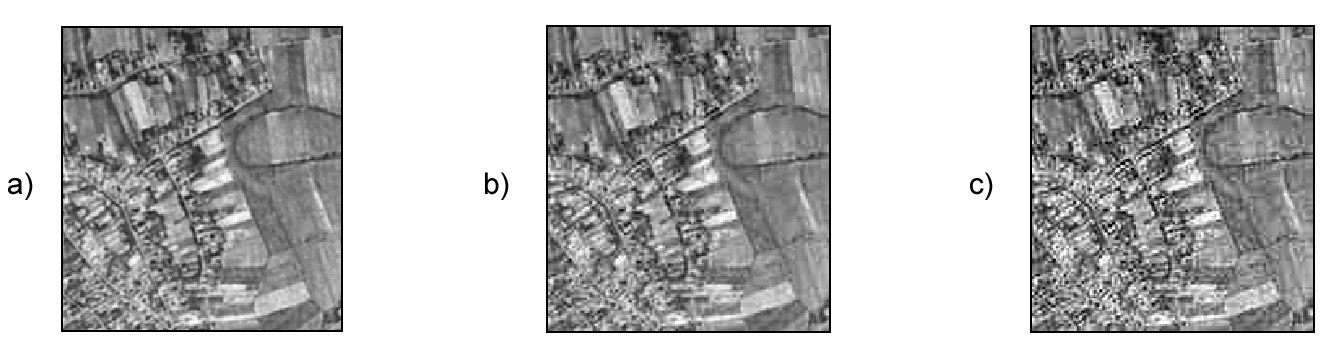
\includegraphics[width=.9\textwidth]{Fuentes_datos/Compresion_con_perdidas.png}
\caption{\small Efectos de la utilizaci�n de algoritmos de compresi�n con p�rdidas. a) Imagen original. b) Imagen almacenada mediante compresi�n con p�rdidas. c) Imagen tras diez procesos de lectura y almacenamiento en un formato de archivo con compresi�n con p�rdidas. El efecto de la degradaci�n sucesiva que la imagen sufre es claramente apreciable.}
\label{Fig:Compresion_con_perdidas} 
\end{figure}

\subsubsection{Formatos para datos SIG}

Junto con los formatos de archivo para im�genes, los SIG r�ster han desarrollado sus propios formatos para el almacenamiento de capas r�ster en general, y en particular de aquellas que no representan im�genes, tales como capas de variables f�sicas.

Estos formatos est�n pensados para las caracter�sticas de estas capas, que habitualmente recogen valores decimales (a diferencia de los valores enteros de los Niveles Digitales de una imagen), y que no suelen contener m�s que una �nica banda.

Adem�s de corresponder a un SIG particular (pr�cticamente cada SIG tiene su propio formato de archivo r�ster), otras aplicaciones que trabajan con este tipo de datos, tales como todas aquellas que usan por una u otra raz�n informaci�n de elevaciones, tambi�n disponen de sus formatos particulares. Muchos SIG pueden leer algunos de estos formatos junto con los suyos propios o los de otros SIG.

A la hora de almacenar una capa tal como un Modelo Digital del Terreno o cualquier otra de similar �ndole, estos formatos son preferibles en general a las im�genes, ya que los formatos de imagen, aunque ya hemos visto que pueden adaptarse y ser en algunos casos plenamente operativos para otro tipo de variables, no son formatos puramente pensados para este tipo de informaci�n.

\subsubsection{Principales formatos existentes}

Dentro de la gran variedad de formatos existentes, he aqu� una breve lista de los principales, los cuales suelen encontrarse con frecuencia a lo largo del desarrollo de un proyecto SIG habitual.

Dentro de los formatos para im�genes, cabe destacar los siguientes:

\begin{itemize}
	\item \textbf{Tagged Image File Format (tif)}. Se trata de un formato complejo y altamente flexible, con muchas variantes distintas. Puede incorporar tanto compresi�n con p�rdidas como sin p�rdidas, en funci�n del algoritmo que se utilice. Se utiliza habitualmente tanto en el �mbito del tratamiento de im�genes como en el �mbito SIG. En este �ltimo, permite tambi�n el almacenamiento de valores decimales, siendo apto para almacenar capas que no representen im�genes como tal.
	Es un formato habitualmente generado por los esc�neres, con lo cual es frecuente su utilizaci�n al trabajar con cartograf�a escaneada, seg�n vimos antes en este mismo cap�tulo.
	Existe una variante denominada GeoTIFF, que permite incorporar en el propio fichero la georreferencia de la imagen, haciendo innecesario el uso de un \emph{World File} asociado.
	\item \textbf{Joint Photographic Experts Group (jpg o jpeg)}. Un formato muy popular para im�genes (todas las c�maras digitales lo utilizan), no es sin embargo adecuado para el trabajo con SIG. Incorpora compresi�n con p�rdidas (el ejemplo de la figura \ref{Fig:Compresion_con_perdidas} ha sido realizado utilizando este formato), y no es apto para almacenar capas r�ster que no sean de tipo imagen.
\end{itemize}
\index{Tagged Image File Format (TIFF)}\index{Joint Photographic Experts Group (JPEG)}\index{GeoTIFF}

Algunos formatos espec�ficos para im�genes SIG tales como im�genes de sat�lite, son:

\begin{itemize}
	\item \textbf{Enhanced Compression Wavelet (ecw)}. Formato desarrollado por Earth Resource Mapping. Al igual que el siguiente, est� especialmente preparado para almacenar im�genes de gran tama�o, ya que las im�genes a�reas o de sat�lite en general tiene tama�os mayores que las im�genes de uso gen�rico para las que est�n pensados los formatos como TIFF o JPEG. 
	En el uso de estas im�genes de gran tama�o en un SIG, es habitual que se quiera acceder a la imagen (por ejemplo para su visualizaci�n) solo en una parte determinada de la misma. Para optimizar este tipo de acceso, el formato soporta acceso sin necesidad de descomprimir la totalidad del archivo (descompresi�n selectiva).
	Se trata de un formato de compresi�n con p�rdidas, y su grado de compresi�n es alto. 
	\item \textbf{Multi--resolution Seamless Image Database (MrSID)} (sid). Al contrario que el anterior, que es un formato abierto, el formato MrSID es un formato cerrado, pero sus caracter�sticas son similares: alta compresi�n, preparado para im�genes de gran volumen y con posibilidad de descompresi�n selectiva.
\end{itemize}
\index{Enhanced Compression Wavelet (ECW)}\index{Multi--resolution Seamless Image Database (MrSID)}

Por �ltimo, entre los formatos para datos r�ster (no im�genes) m�s comunes destacar el siguiente:

\begin{itemize}
	\item \textbf{ArcInfo ASCII (asc)}. Un formato en texto plano ASCII\footnote{\emph{American Standard Code for Information Interchange}. Un esquema de codificaci�n de caracteres ampliamente utilizado.}. �nicamente soporta una �nica banda, y permite almacenar el valor a considerar como valor de sin datos.
\end{itemize}
\index{ArcInfo ASCII (formato)}\index{American Standard Code for Information Interchange (ASCII)}

\subsection{Formatos para datos vectoriales}

Sin ser tan abundantes como los formatos para datos r�ster, existe tambi�n un buen n�mero de formatos de archivo para datos vectoriales. Al igual que en el caso r�ster, estos formatos de archivo no derivan �nicamente de los SIG, sino tambi�n de otras aplicaciones que utilizan capas de tipo vectorial, con  particular importancia de las de dise�o asistido por ordenador (CAD).

A la hora de definir las caracter�sticas de un formato de archivo para datos vectoriales, encontramos dos aspectos principales, a saber:

\begin{itemize}
	\item Capacidad para recoger la topolog�a de la capa
	\item Capacidad para recoger los atributos de las entidades.
\end{itemize}

En el primer aspecto, debemos considerar que existen SIG no topol�gicos, es decir, que no son capaces de manejar informaci�n sobre la topolog�a de la capa, y por tanto no la necesitan. Los formatos de archivo de estos SIG no estar�n por tanto pensados para trabajar con topolog�a, y por ello no la almacenan.

Respecto a la capacidad para recoger los atributos de una capa, este aspecto afecta principalmente a los formatos propios de las aplicaciones CAD. En estas, la componente espacial es la que prima, no teniendo tanta relevancia la componente tem�tica. Los puntos, l�neas y pol�gonos con los que se trabaja en un CAD no tiene atributos asociados salvo aquellos relacionados con su propia representaci�n tales como color, grosor o estilo. Existen formas de asociar una componente tem�tica a esas entidades, pero estas son variadas y la interoperabilidad disminuye en caso de emplearlas, ya que no est�n soportadas con car�cter general en los distintos SIG. 

Por esta raz�n, estos formatos son aptos para introducir informaci�n dentro de un SIG o para exportarla a un CAD con objeto de utilizar capacidades de este que no se tengan en el SIG, pero como formatos de almacenamiento de datos dentro de un SIG no son los m�s id�neos, y debe optarse por otros m�s espec�ficos para datos SIG.

\subsubsection{Principales formatos existentes}

Los formatos m�s extendidos para datos SIG vectoriales son los siguientes:

\begin{itemize}
	\item \textbf{Shapefile (shp)}. Propuesto por la empresa ESRI, es el formato m�s utilizado en la actualidad, convertido en un est�ndar \emph{de facto}. No soporta topolog�a y se compone de diversos ficheros, cada uno de los cuales contiene distintos elementos del dato espacial (geometr�as, atributos, �ndices espaciales, etc.)
	\item \textbf{Spatialite}. Una extensi�n espacial para la base de datos \emph{SQLite}. Se trata de una base de datos, pero no tiene la arquitectura cl�sica de esta, con aplicaci�n cliente y un servicio que provee los datos (lo veremos con m�s detalle en el cap�tulo \ref{Bases_datos}), sino que toda ella se encuentra almacenada en un fichero que puede copiarse o eliminarse de la forma habitual.
	\item \textbf{GeoJSON}. Un formato de texto plano basado en notaci�n JSON\footnote{JavaScript Object Notation}, de uso extendido debido a su simplicidad. Existe una variante denominada TopoJSON, que permite el almacenamiento de topolog�a.
\end{itemize}

\section{Resumen}

Los datos con los que trabajamos en un SIG pueden venir de muy distintas procedencias. Distinguimos aquellos que provienen directamente de alg�n tipo de medida o del empleo directo de alguna instrumentaci�n (fuentes de datos primarias), y otros que proceden de procesar un dato ya existente para adaptarlo a su uso en un SIG (fuentes de datos secundarias).

Una forma b�sica de crear datos espaciales digitales es la utilizaci�n de fuentes no digitales y su digitalizaci�n. Este proceso puede llevarse a cabo tanto de forma manual como automatizada, y puede dar como resultado tanto capas r�ster como capas vectoriales.

La teledetecci�n es una fuente de datos de gran importancia para los SIG. Dentro de ella se incluyen t�cnicas de muy diversa �ndole cuyos productos son muy distintos entre s�. El fundamento de la teledetecci�n es la medici�n de las propiedades de los objetos realizada sin que medie contacto con estos. Para ello, se emplean sensores que pueden ir a bordo de aviones o montados sobre sat�lites, y que pueden ser de tipo pasivo o activo. El resultado del proceso de teledetecci�n son im�genes con un n�mero variable de bandas, aunque tecnolog�as como el radar o el LiDAR pueden emplearse para la generaci�n de cartograf�a de elevaciones.

Dentro de las tecnolog�as que permiten la recogida de datos en campo, el GPS ha supuesto un cambio en la realizaci�n de este tipo de trabajos, y su integraci�n en SIG es sencilla. Esto les ha convertido en una fuente de datos muy utilizada en un gran n�mero de proyectos SIG.

Independientemente de su origen, los datos espaciales se almacenan en archivos cuyos formatos son a su vez muy variados. En este cap�tulo hemos visto algunos de los m�s habituales, as� como los aspectos m�s importantes que los definen, y que han de tenerse en cuenta a la hora de trabajar con dichos formatos y elegir los m�s adecuados.

\pagestyle{empty}

\chapter{Software y teconolog�a}
\label{Software}


\pagestyle{fancy}


El concepto cl�sico de un SIG es el de una aplicaci�n completa en la cual se implementan herramientas para llevar a cabo las tareas b�sicas del trabajo con datos geogr�ficos: creaci�n o edici�n, manejo y an�lisis. Junto a este enfoque tradicional, con el tiempo han surgido otras formas distintas de aplicaciones que tambi�n pueden considerar como parte del �mbito del SIG. 

Veremos en este cap�tulo las caracter�sticas de las aplicaciones SIG, divididas en tres grupos fundamentales: herramientas de escritorio, cartograf�a en la Web (\emph{Web--mapping}) y SIG m�vil. Asimimoso, veremos algunos aspectos tecnol�gicos relacionados con ellas.


\section{Herramientas de escritorio}

Podemos dividir las funciones b�sicas de un SIG de escritorio en cinco bloques: \textbf{entrada y salida de datos, visualizaci�n, edici�n, an�lisis y generaci�n de cartograf�a}. Una aplicaci�n de escritorio habitual presenta todas estas capacidades en cierta medida, aunque no necesariamente con el mismo nivel de implementaci�n.

\subsection{Entrada y salida de datos}

Una aplicaci SIG de escritorio debe implementar capacidades para leer datos y, opcionalmente, para guardarlos. Esta ultima es necesaria en el caso en que el SIG pueda generar nuevos datos geogr�ficos (nuevas capas), pero no en aquellas aplicaciones sin capacidades de an�lisis o edici�n, donde su empleo no ha de crear nuevos datos.

La existencia de librer�as y componentes de acceso a datos en los que las aplicaciones SIG de escritorio pueden apoyarse permite dar soporte al gran n�mero de formatos de datos existentes, mejorando la \textbf{conectividad} entre estas.

Adem�s de acceder a ficheros de datos, en la actualidad es importante poder acceder a \textbf{bases de datos} o \textbf{servicios remotos}. Hablaremos de  estos �ltimos m�s adelante dentro de este cap�tulo.

\subsection{Visualizaci�n}
\label{Funcion_SIG_Visualizacion}

La visualizaci�n es una funci�n fundamental dentro de los SIG y del trabajo con cartograf�a en general. Tiene importancia cuando la representaci�n de los datos es el prop�sito principal de utilizar un SIG, pero tambi�n cuando el trabajo est� enfocado a la edicion o la realizaci�n de an�lisis, ya que la visualizaci�n y exploraci�n visual de los datos de partida es un paso previo.


Esta estructura se compone fundamentalmente de un lienzo sobre el que se sit�an las distintas capas de informaci�n geogr�fica, y que el usuario va conformando a�adiendo nuevas capas y editando la forma en la que estas se representan. Las capas se sit�an en un orden dado dentro del lienzo, lo que permite establecer una jerarqu�a de representaci�n y as� lograr el aspecto deseado.

Junto a este lienzo existen herramientas de navegaci�n que permiten ampliar o reducir la escala, o bien modificar el encuadre (Figura \ref{Fig:Herramientas_navegacion}). 

\begin{figure}[!hbt]
\centering
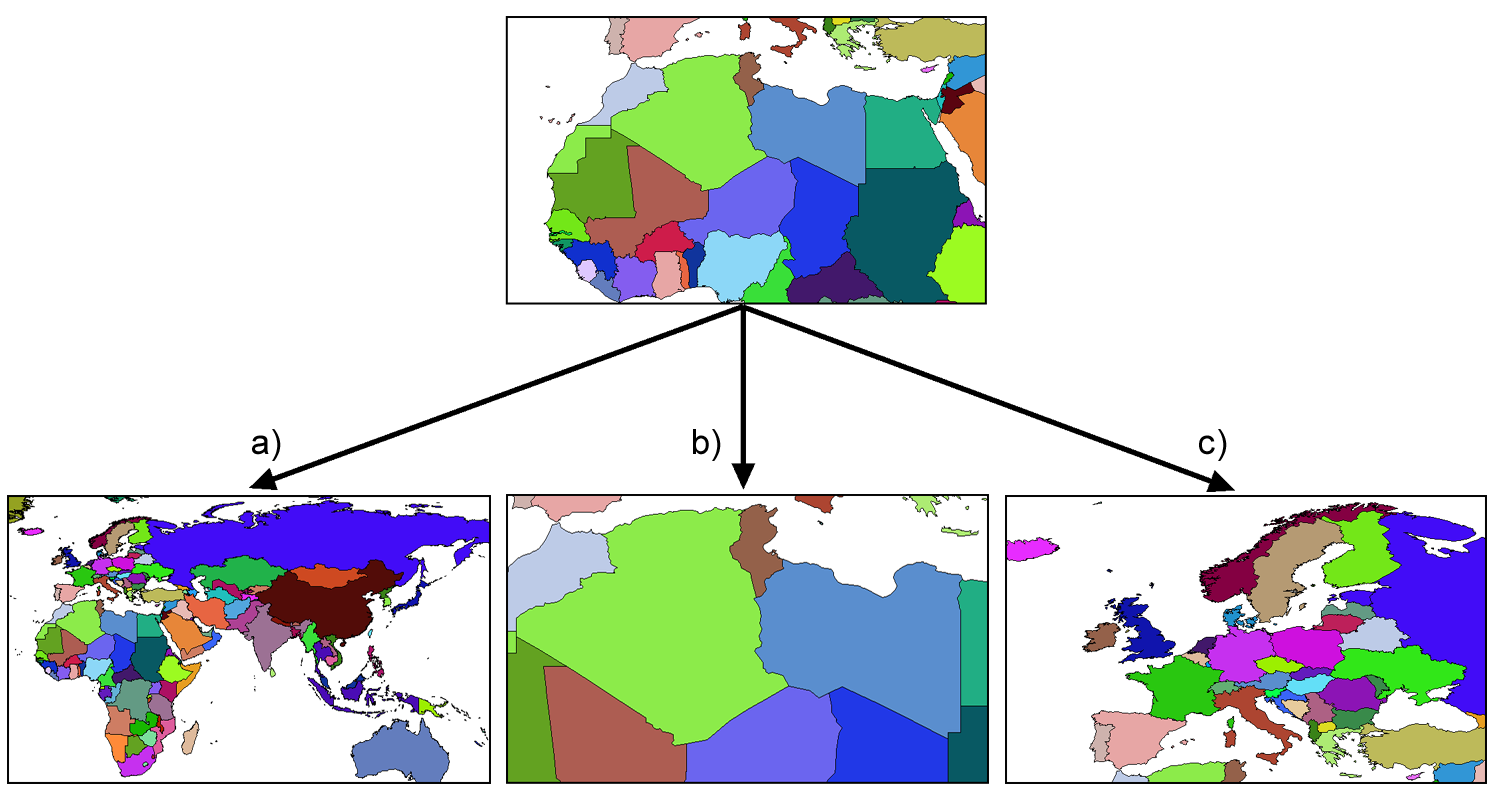
\includegraphics[width=.99\textwidth]{Software/Herramientas_navegacion.png}
\caption{\small Herramientas de navegaci�n fundamentales en el entorno gr�fico de un SIG de escritorio. a) alejamiento (\emph{zoom out}), b) acercamiento (\emph{zoom in}), c) desplazamiento (\emph{pan})}
\label{Fig:Herramientas_navegacion} 
\end{figure}

El aspecto m�s destacable de la visualizaci�n de datos espaciales en un SIG es que, a diferencia de un mapa cl�sico donde no pueden modificarse sus caracter�sticas, el usuario puede aqu� de forma r�pida y sencilla elegir \emph{qu�} ve y \emph{c�mo} lo ve. El dato espacial digital es independiente de la informaci�n necesaria para su representacion (colores, texturas, etc.), y un mismo dato puede por tanto representarse de maneras diferentes. Esto es particularmente cierto para el caso de capas vectoriales, as� como para capas r�ster que contengan un valor de tipo no gr�fico, es decir, aquellas que no sean im�genes.

Aunque en el caso m�s habitual, la representaci�n de una capa en un lienzo de un SIG es bidimensional, de la misma forma que se representa en un mapa impreso, existen tambien SIGs con capacidades de visualizaci�n tridimensional. En este caso, las herramientas de navegaci�n son m�s complejas, existiendo ajustes relativos a la perspectiva, a los �ngulos de visi�n o a la exageraci�n del relieve, entre otros par�metros. 






\subsection{An�lisis}

Si hubi�ramos de ordenar cronol�gicamente las distintas funcionalidades que un SIG de escritorio presenta, probablemente el an�lisis fuera una de las primeras. Por encima de otras capacidades, los ordenadores han sido y son principalmente herramientas de c�lculo capaces de realizar operaciones y computar resultados, y este ha sido uno de los usos fundamentales relativos al manejo de datos geogr�ficos. Otros usos, tales como la visualizaci�n, pese a ser pr�cticamente imprescindibles hoy en d�a, estaban muy limitados en los primeros SIG. No ocurr�a as� en el �mbito del an�lisis ya que, aunque con capacidades como es l�gico menores que las actuales, los ordenadores ofrec�an una potencia de calculo que los convert�a en herramientas de an�lisis tan interesantes como en la actualidad.

La tendencia actual en los SIG es considerar las capacidades de an�lisis como herramientas modulares que se ejecutan sobre una plataforma base, la cual comprende las capacidades de visualizaci�n y entrada y salida de datos. Todas estas capacidades de an�lisis son independientes entre s�, aunque pueden coordinarse y emplearse en conjunto para alcanzar un resultado concreto. De otro modo, cada una de las formulaciones o algoritmos que vimos en cap�tulos anteriores aparece dentro del SIG como una herramienta individual que opera sobre una serie de capas y genera un resultado dado, tomando en muchas ocasiones esas capas de entre aquellas que se est�n representando en el SIG, e incorporando asimismo a dicha representaci�n las nuevas capas generadas.

Las herramientas de an�lisis pueden aparecer igualmente como programas independientes, y el SIG de escritorio ser una herramienta aglutinadora que centraliza estas, facilitando su uso y la gesti�n de los datos implicados en los procesos de an�lisis.

Cuando las herramientas de an�lisis utilizan directamente la base del SIG donde se encuentran las capacidades de visualizaci�n y manejo de datos, puede existir cierto grado de interactividad. Las operaciones de consulta, por ejemplo, las cuales vimos en el cap�tulo \ref{Consultas}, son en general de este tipo, ya que el usuario puede actuar sobre el lienzo para hacer una selecci�n de modo gr�fico. M�s a�n, esa selecci�n puede condicionar los posteriores an�lisis sobre la capa cuyas entidades se seleccionan, ya que los procesos que operen sobre ella pueden restringir su alcance a aquellas entidades seleccionadas.\index{Consultas}

En caso de no existir este tipo de interacci�n entre elementos de an�lisis y elementos de visualizaci�n y exploraci�n de datos, los procesos de an�lisis suelen constituir utilidades autocontenidas que simplemente toman una serie de datos de entrada, realizan un proceso en el que el usuario no interviene, y finalmente generan un resultado con car�cter definitivo. Este resultado podr� ser posteriormente visualizado o utilizado como entrada para un nuevo an�lisis.

A modo de ejemplo, podemos analizar el caso particular del c�lculo de una ruta que conecte una serie de puntos a trav�s de una red (los fundamentos de este an�lisis los vimos en el apartado\ref{Analisis_redes}). \index{Ruta �ptima}

Una de las formas de implementar este an�lisis es aquella que requiere del usuario la introducci�n de la informaci�n necesaria (una capa de lineas con la red viaria y otra de puntos con los puntos de inicio, paso, y llegada correspondientemente ordenados) como par�metros que el proceso toma y en funci�n a los cuales se genera una nueva capa. El proceso es una tarea perfectamente definida, con unas entradas y una salidas, y tras la selecci�n de unas capas de entrada se genera un nuevo resultado en forma de otra capa. Este proceso puede implementarse de forma aislada del SIG, aunque coordinada con �l para lograr mejores resultados y una utilizaci�n m�s sencilla.\index{Interactividad}

Otra forma con un enfoque distinto ser�a presentando un proceso interactivo en el cual se introduce como �nico par�metro inicial la red viaria. Posteriormente, el usuario puede operar sobre el lienzo en el que esta se encuentra representada para ir definiendo y editando la lista de puntos de paso. El c�lculo se va efectuando cuando se produce alg�n cambio en la misma y debe aplicarse de nuevo el algoritmo pertinente para adaptar el resultado ---la ruta �ptima--- a ese cambio.

Este tipo de formulaciones interactivas son m�s intuitivas y agradables de usar, pero en realidad menos productivas de cara a un trabajo dentro de un proyecto SIG. Aparecen por ello en aquellas funciones que tienen una mayor componente visual o, especialmente, en las que representan un an�lisis puntual que se realiza de forma com�n como algo individual. Estos son los an�lisis que se implementan en las aplicaciones que veremos m�s adelante como parte del grupo de SIG enfocados a la exploraci�n visual de datos geogr�ficos, que adem�s de esta proveen alguna serie de utilidades de an�lisis, pocas en general, sin que estas est�n concebidas para un trabajo completo en un proyecto SIG de cualquier �ndole, sino m�s bien para un uso ocasional.

En un proyecto SIG de cierto tama�o, lo m�s com�n es que la fase de an�lisis, a la que seguir� una fase tambi�n compleja de preparaci�n e interpretaci�n de resultados, y previa a la cual se ha debido llevar a cabo la preparaci�n de los datos de partida, comprenda no uno, sino muchos an�lisis distintos. Estos an�lisis, a su vez, no son independientes, sino que est�n relacionados entre s� y lo m�s habitual es que definan como tales un flujo de trabajo que comienza en los datos de partida y desemboca en los resultados finales a trav�s de una serie de procesos. 

Por su naturaleza, tanto los datos espaciales como los procesos en los que estos intervienen se prestan a formar parte de estos flujos de trabajo m�s o menos complejos, y es por ello que en los SIG actuales una funcionalidad b�sica es la creaci�n de tareas complejas que permiten simplificar todo un proceso de muchas etapas en una �nica que las engloba a todas. La forma anteriormente comentada en que aparecen las formulaciones dentro de un SIG, de forma atomizada y modular, facilita la creaci�n de estos <<modelos>> a partir de procesos simples.

Para entender esta idea, podemos ver un ejemplo aplicado. La extracci�n de una red de drenaje en formato vectorial a partir de un MDE requiere una serie de procesos, a saber (para repasar los fundamentos de cada uno de estos procesos y comprender mejor la operaci�n global, puede consultarse el cap�tulo \ref{Geomorfometria}, donde se describieron en su momento, as� como la secci�n \ref{Vectorizacion_lineas}):

\begin{enumerate}
	\item Eliminaci�n de depresiones del MDE.
	\item C�lculo de una capa de �rea acumulada a partir del MDE corregido
	\item Extracci�n de capa r�ster con la red de drenaje a partir de la capa anterior y un valor umbral
	\item Vectorizaci�n de la capa resultante del paso anterior
\end{enumerate}

\index{Modelo Digital de Elevaciones}

Lo anterior podr�a simplificarse si se agruparan en una sola operaci�n todos los procesos anteriores, de forma que tomando dos datos de entrada (un MDE y un umbral), se realizara todo el proceso de forma continua. Las capacidades de creaci�n de modelos que implementan los SIG de escritorio (en particular, los m�s enfocados al an�lisis) permiten crear nuevos procesos compuestos utilizando entornos gr�ficos intuitivos, y estos procesos pasan a formar parte del conjunto de ellos de que dispone el SIG, permitiendo que cada usuario <<resuma>> en procesos unitarios una serie de operaciones que, de otro modo, deber�an realizarse de forma individual con el coste operacional que ello implica.

Una vez que se ha creado un proceso compuesto, este puede aplicarse sobre nuevos datos de entrada, reduci�ndose as� el tiempo y la complejidad con que nuevos par�metros de entrada pueden ser procesados seg�n el esquema de trabajo definido en dicho proceso.

Debe pensarse que el proceso presentado como ejemplo es muy sencillo y �nicamente implica cuatro operaciones encadenadas de forma lineal. Un proceso de an�lisis habitual puede contener muchas m�s operaciones individuales, y estas disponerse de forma m�s compleja, con dependencia de distinta �ndole entre sus resultados. 

La imagen \ref{Fig:Proceso_complejo} muestra el aspecto de uno de tales procesos implementado en QGIS, un software GIS con capacidad de de creaci�n de modelos. El proceso representado en la figura \ref{Fig:Esquema_MonteCarlo} tambi�n es un ejemplo de otro tipo de an�lisis que puede adaptarse ventajosamente en este tipo de herramientas de modelizaci�n.


\begin{figure}[!hbt]
\centering
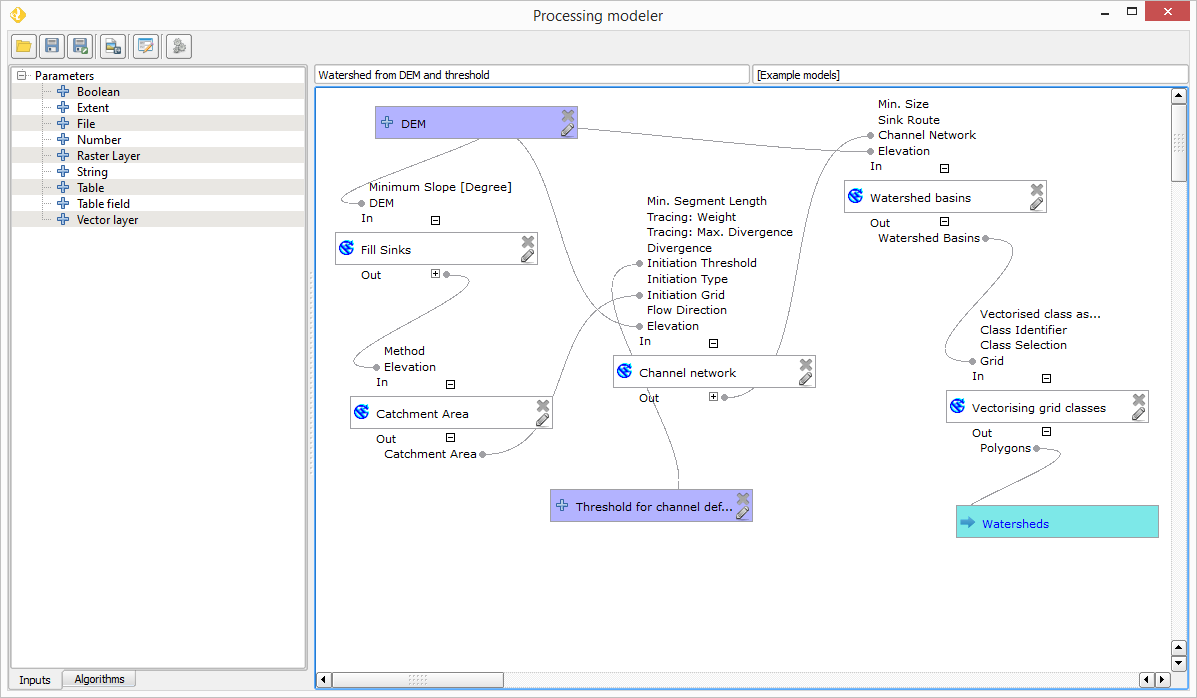
\includegraphics[width=.9\textwidth]{Software/Proceso_complejo.png}
\caption{\small Esquema de un proceso complejo creado a partir de operaciones simples de an�lisis con datos SIG.}
\label{Fig:Proceso_complejo} 
\end{figure}

Asimismo, las herramientas SIG que contienen funcionalidad de an�lisis suelen permitir el acceso a estas a traves de lenguajes de \emph{scripting}, lo cual facilita la creaci�n de flujos de trabajo y la automatizaci�n de rutinas complejas de an�lisis. Si bien este trabajo no se realiza de un modo gr�fico e intuitivo como en el ejemplo mostrado anteriormente, y requiere mayores conocimientos, la flexibilidad y potencia que ofrece es mucho mayor.







\subsection{Edici�n}


Los datos geogr�ficos con los que trabajamos en un SIG no son una realidad est�tica. La informaci�n contenida en una capa es susceptible de ser modificada o corregida, y las funciones que permiten estas tareas son importantes para dotar al SIG de versatilidad. Sin ellas, los datos espaciales pierden gran parte de su utilidad dentro de un SIG, ya que se limitan las posibilidades de trabajo sobre estos. Las funcionalidades de edici�n son, por tanto, b�sicas en una herramienta de escritorio.

Las operaciones de edici�n pueden emplearse para la creci�n de nueva cartograf�a (como vimos en el cap�tulo \ref{Fuentes_datos}), as� como para la actualizaci�n de esta. 

Aunque las tareas de edici�n m�s habituales son las relacionadas con la edici�n de geometr�as, no es esta la �nica edici�n que puede realizarse dentro de un SIG. Podemos distinguir las siguientes formas de edici�n:

\begin{itemize}
\item Edici�n de geometr�as de una capa vectorial.
\item Edici�n de atributos de una capa vectorial, incluyendo la adici�n o eliminaci�n de atributos en toda una capa.
\item Edici�n de valores de una capa r�ster.
\end{itemize}

Las herramientas destinadas a la edici�n de entidades geom�tricas heredan sus caracter�sticas de los programas de dise�o asistido por ordenador (CAD), cuya funcionalidad principal es precisamente la edici�n de elementos gr�ficos. Aparecen en algunos casos herramientas adicionales, como sucede en el caso de que se registre informaci�n topol�gica.



\subsection{Generaci�n de cartograf�a}
\label{GeneracionCartografia}

La mayor�a de las herramientas de escritorio incorporan capacidades de creaci�n de cartograf�a impresa, generando un documento cartogr�fico que posteriormente puede imprimirse y emplearse como un mapa cl�sico. Estas capacidades permiten la composici�n de documentos cartogr�ficos de acuerdo con un dise�o dado, y la impresi�n directa de estas en alg�n perif�rico tal como una impresora com�n o un \emph{plotter} de gran formato. 

Las funciones de dise�o que se implementan por regla general en un SIG son similares a las que pueden encontrarse en un software de maquetaci�n gen�rico, permitiendo la composici�n gr�fica del documento general y el ajuste de los distintos elementos que lo forman. Entre estos elementos, destaca el mapa como tal, es decir, aquel que contiene la representaci�n del dato geogr�fico.

Junto a esto, las herramientas de escritorio incluyen funcionalidades para automatizar la producci�n cartogr�fica, tales como la creaci�n de plantillas o las generaci�n de series de mapas que cubren en su conjunto una amplia extensi�n, fragmentando esta en unidades (Figura \ref{Fig:Serie_mapas})

\begin{figure}[!hbt]
\centering
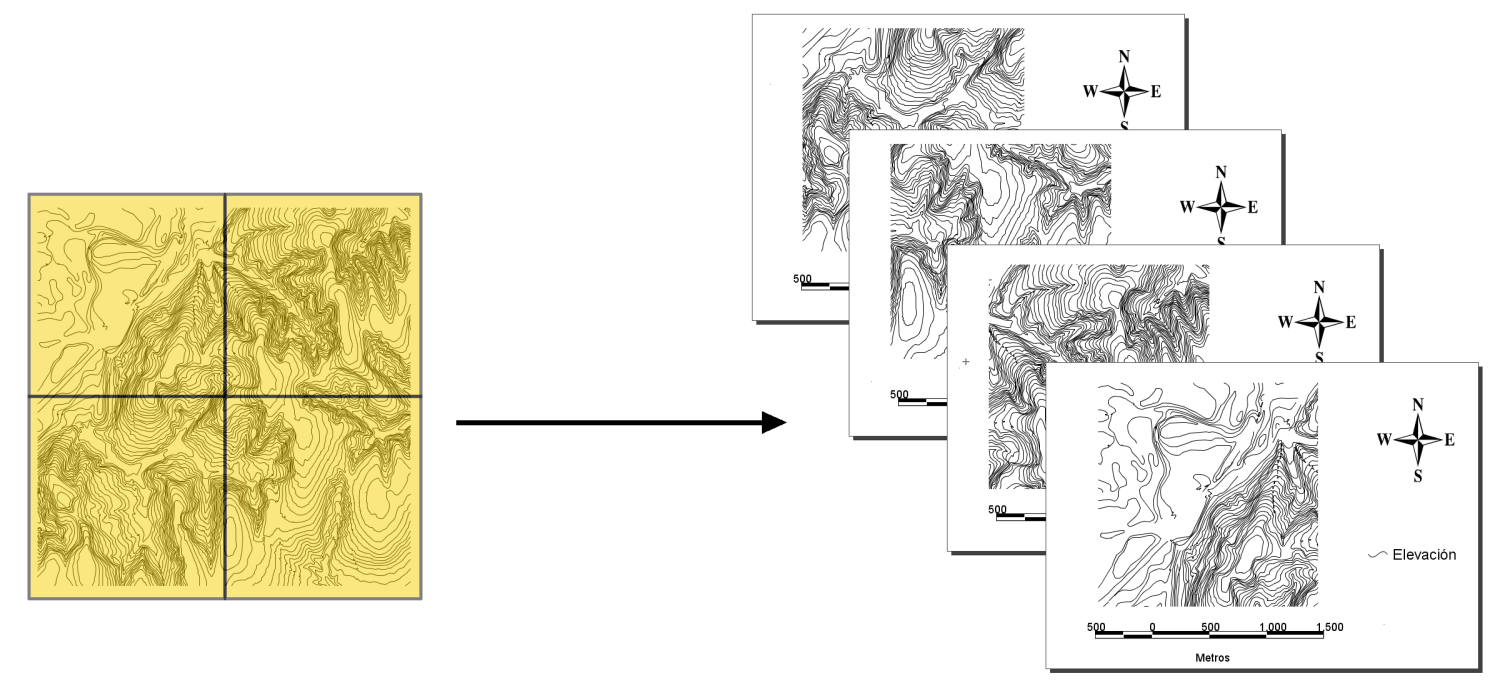
\includegraphics[width=.9\textwidth]{Software/Serie_mapas.png}
\caption{\small La automatizaci�n de las tareas de creaci�n cartogr�fica permite simplificar la producci�n de grandes vol�menes de cartograf�a, como por ejemplo al dividir un �rea geogr�fica en una serie dada de mapas.}
\label{Fig:Serie_mapas} 
\end{figure}

Estas posibilidades surgen de la \textbf{separaci�n entre los datos espaciales y el dise�o del documento cartogr�fico} que los contiene, del mismo modo que ya vimos que existe entre datos y par�metros de representaci�n a la hora de visualizar los primeros.


\section{Cartograf�a en la Web (\emph{Web--mapping}). Clientes y servidores}


Uno de los avances m�s importantes en la historia de los SIG lo constituye la llegada del \emph{Web Mapping}. Entendemos como tal a las tecnolog�as que permiten incorporar las ideas de los SIG dentro de paginas Web, utilizando un navegador Web como aplicaci�n principal. Asimismo, estas tecnolog�as, junto a la importancia de Internet, han propiciado el desarrollo de otros elementos tecnol�gicos tales como servicios de datos remotos, que se utilizan tanto en las aplicaciones de escritorio como en el propio \emph{Web Mapping}.

Los conceptos de \textbf{servidor} y \textbf{cliente} son fundamentales en este contexto. Veamos algunas ideas generales al respecto.

Conocemos como \emph{servidor} al elemento encargado de \emph{servir} alg�n tipo de contenido. En el �mbito SIG, se trata fundamentalmente de datos geogr�ficos, que constituyen el principal producto que se distribuye a trav�s de la red dentro de nuestro campo. 

El \emph{cliente} es responsable de \emph{pedir} ese dato al servidor, tomarlo y trabajar con �l. Un navegador Web es un cliente, ya que  realiza una petici�n para mostrar una p�gina Web. Al introducir una direccion Web en la barra de direcciones del navegador, proporcionamos una serie de datos que son los que se emplean para realizar el proceso, y que vamos a ver a continuaci�n en detalle.

Supongamos la direcci�n Web \texttt{http://victorolaya.com/writing}. Al visitar esa p�gina, se efectua una petici�n a trav�s de su direcci�n, la cual se compone de las siguientes partes:

\begin{itemize}
	\item \texttt{http}: El protocolo a usar, que define la forma en que se van a comunicar cliente y servidor.
	\item \texttt{victorolaya.com}: Esta cadena identifica la m�quina donde reside la p�gina que buscamos. Es en realidad una versi�n m�s legible para el ojo humano de un c�digo num�rico que indica la direcci�n concreta. 
	\item \texttt{writing}: La p�gina que buscamos dentro de todas las que hay en esa m�quina. 
\end{itemize}
\index{FTP}

El proceso mediante el que podemos ver esa p�gina en un navegador Web comprende los cuatro pasos siguientes:

\begin{enumerate}
	\item El cliente realiza la petici�n.
	\item La petici�n se conduce a trav�s de la red hasta el servidor.
	\item El servidor busca la p�gina y la devuelve a trav�s de la red en caso de encontrarla, o devuelve una pagina de error en caso de no tenerla.
	\item El cliente recibe la p�gina y la representa.
\end{enumerate}


La figura \ref{Fig:Asi_funciona_internet} muestra un esquema de este proceso.

\begin{figure}[!hbt]   
\centering
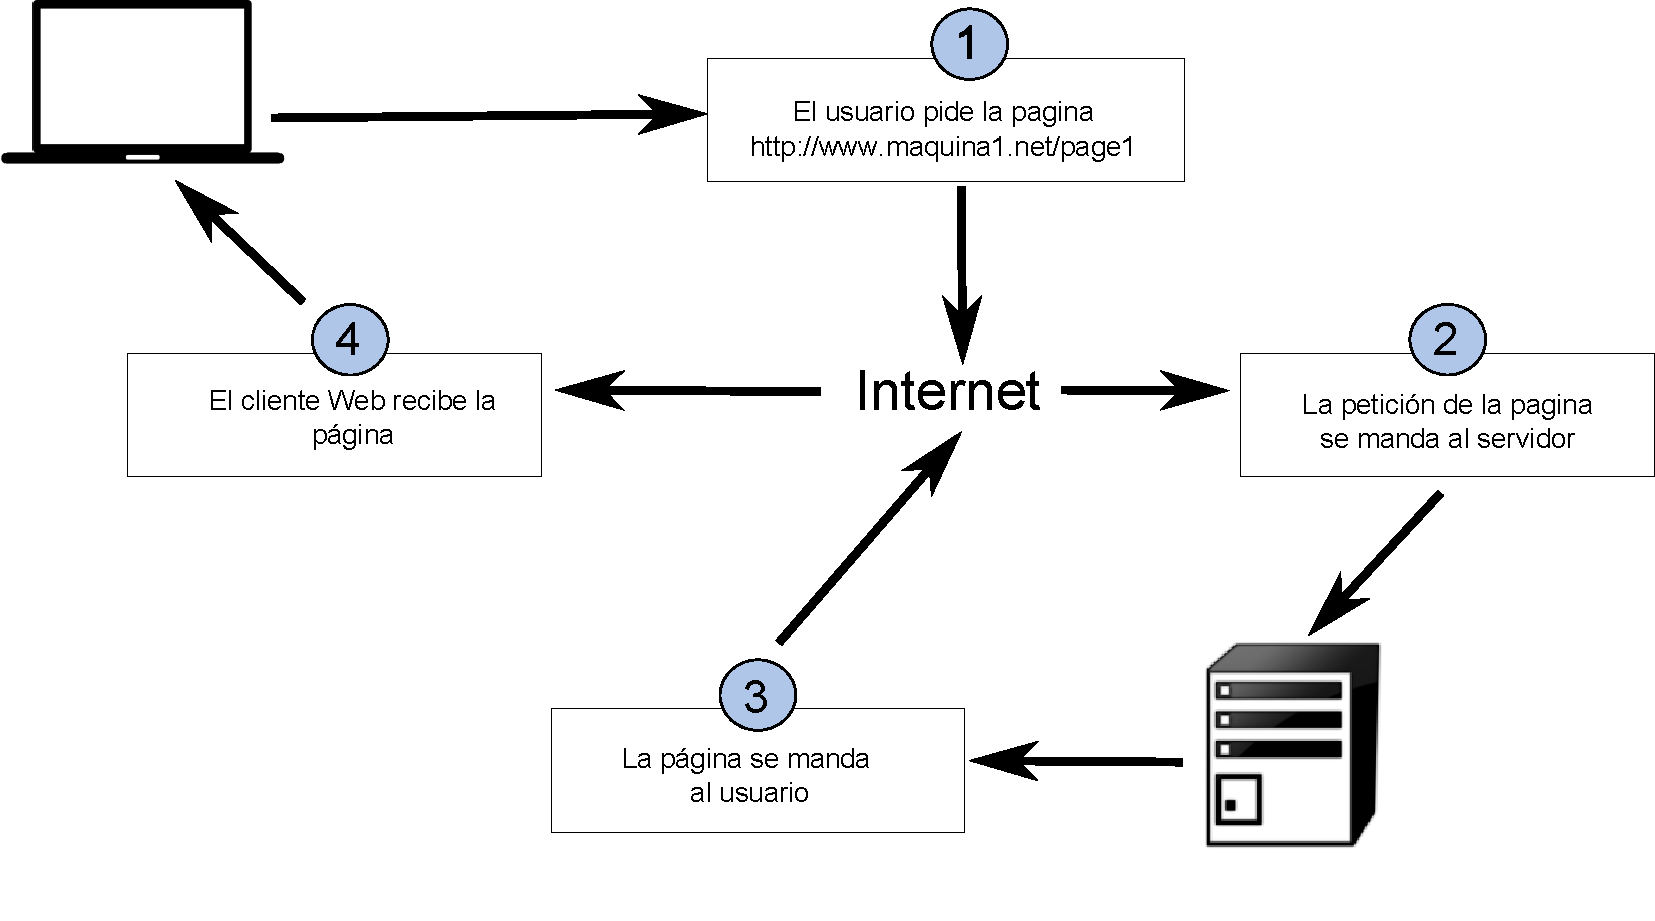
\includegraphics[width=.95\mycolumnwidth]{Cliente_servidor/Asi_funciona_internet.pdf}
\caption{\small Esquema del proceso de consulta de una p�gina Web desde un navegador.}
\label{Fig:Asi_funciona_internet} 
\end{figure}

De modo gr�fico, la relaci�n entre ambos elementos puede representarse seg�n la figura \ref{Fig:Servidores_y_clientes}. En ella, un n�mero variable de clientes se <<conectan>> a un servidor, del cual obtienen una serie de datos cuando este responde a las peticiones formuladas por cada uno de los clientes. En la arquitectura cliente--servidor, este �ltimo es el que posee la informaci�n a compartir a trav�s de los servicios, mientras que en cada uno de los clientes se almacena tan solo la informaci�n personal de estos.

\begin{figure}[!hbt]   
\centering
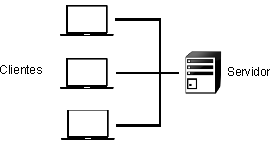
\includegraphics[width=0.75\mycolumnwidth]{Cliente_servidor/Servidores_y_clientes.pdf}
\caption{\small Relaci�n entre clientes y servidores.}
\label{Fig:Servidores_y_clientes} 
\end{figure}

Veamos ahora algunas caracter�sticas de los servidores y clientes dentro del �mbito SIG.

Respecto a los servidores, las capacidades fundamentales en este contexto pueden dividirse en los siguientes grupos:

\begin{itemize}
\item \textbf{Servir representaciones de los datos}. Los servicios de cartograf�a Web, tanto en sus or�genes como en la actualidad, son eminentemente gr�ficos, y en �ltima instancia lo que la aplicaci�n Web correspondiente va a hacer es mostrarnos alg�n tipo de imagen con un mapa formado a partir de una serie de datos geogr�ficos. El servidor puede responder directamente a este tipo de necesidades, preparando una imagen a partir de los datos geogr�ficos de los que dispone. En el caso de que estos sean ya im�genes ---por ejemplo, im�genes de sat�lite u ortofotos---, bastar� servir estas, transmitiendo una versi�n escalada de las dimensiones exactas que el cliente necesite para representar en pantalla. En caso de que los datos sean de tipo vectorial, o bien r�ster sin una forma de representaci�n impl�cita ---por ejemplo, un Modelo Digital del Terreno--- es necesario emplear alg�n m�todo para asignarles dicha representaci�n. Este puede ser asignado por defecto por el servidor, que establecer� una simbolog�a fija, o bien ofrecer un servicio m�s complejo en el que el cliente no solo pide una representaci�n gr�fica de una serie de datos para una zona dada, sino que adem�s puede especificar \emph{c�mo} crear esa representaci�n.\index{Modelo Digital del Terreno}\index{Ortofotograf�a}

Asimismo, el servidor puede ofrecer la posibilidad de seleccionar los datos empleados para crear la representaci�n gr�fica. En t�rminos de un SIG de escritorio esto es equivalente a seleccionar qu� capas se van a representar de entre el total de las que se encuentran abiertas o bien en nuestro cat�logo de datos al que tenemos acceso desde el SIG. En el caso de un servicio Web, el servidor dispone de una serie de capas a las que puede acceder, y a la hora de servir una imagen puede preparar esta usando unas u otras seg�n las necesidades que el cliente especifique a la hora de hacer la petici�n del servicio. De igual modo, el orden en que se desea que las capas se pinten en el mapa tambi�n debe poder ser especificado por el cliente.

\item \textbf{Servir los datos directamente}. Una opci�n m�s flexible que lo anterior es que el servidor provea directamente los datos geogr�ficos y sea despu�s el cliente quien los utilice como corresponda, bien sea simplemente represent�ndolos ---en cuyo caso deber�a ser el propio cliente quien establezca la simbolog�a, ya que esta tarea ya no queda en manos del servidor--- o bien trabajando con ellos de cualquier otra forma, como por ejemplo analiz�ndolos. 

Aunque las posibilidades son mayores en este caso, se requieren por parte del cliente unas capacidades mayores, ya que mientras que representar una imagen es algo sumamente sencillo desde el punto de vista t�cnico, crear esta a partir de los datos geogr�ficos es m�s complejo.

\item \textbf{Servir consultas}. Un paso m�s all� en la funcionalidad que puede ofrecer el servidor es responder a \emph{preguntas} realizadas por el cliente relativas a los datos, ya sean estas relativas a la parte espacial de dichos datos, o bien a su componente tem�tica. El servidor puede ofrecer como respuesta conjuntos reducidos de los datos de los que dispone, o valores que describan a estos. Estas consultas pueden ser �tiles, por ejemplo, para establecer filtros previos cuando se dispone de un conjunto amplio de or�genes de datos. Un cliente Web puede obtener datos de distintos servidores, y puede consultar si, para un zona dada, estos servidores disponen de informaci�n, sin m�s que consultar la extensi�n cubierta por los datos de cada uno de ellos y comprobar si se interseca con la regi�n de inter�s. En funci�n de la respuesta, puede o no realizarse posteriormente el acceso a los datos en s�. Como ya vimos en el cap�tulo \ref{Metadatos}, los \emph{metadatos} son de gran utilidad para conseguir que este tipo de consultas se realicen de forma eficiente.\index{Metadatos}\index{Consultas}

\item \textbf{Servir procesos}. Por �ltimo, un servidor puede ofrecer nuevos datos, espaciales o no espaciales, resultantes de alg�n tipo de proceso o c�lculo a partir de datos espaciales. En este caso, el proceso constituye en s� el servicio ofrecido por el servidor, y el cliente debe definir los par�metros de entrada de este y los posibles par�metros de ajuste que resulten necesarios. Los datos con los que se trabaja pueden ser proporcionados por el cliente, incorpor�ndolos a su propia petici�n, o bien pueden residir en el propio servidor. En este �ltimo caso, el servidor ofrece tanto los datos, como la posibilidad de extraer resultados a partir de ellos, es decir, los datos y una herramienta para explotarlos. Tambi�n pueden emplearse datos en un servidor distinto, a los que el servidor de procesos puede acceder si estos est�n disponibles, convirti�ndose en cliente de ese segundo servidor (Figura \ref{Fig:Datos_y_procesos_remotos}).

Las posibilidades que estos servicios brindan son muy numerosas. Por una parte, pueden a�adirse funcionalidades avanzadas a interfaces Web, llevando a estas las capacidades propias de los SIG de escritorio. Por otra, la difusi�n de algoritmos de an�lisis geogr�fico resulta m�s sencilla, pudiendo ofrecerse estos a todo tipo de usuarios sin necesidad de ning�n software especializado. Y por �ltimo, en ciertos casos pueden rebajarse los tiempos de proceso, ya que, en el caso de operaciones complejas, la mayor potencia del servidor respecto al cliente puede resultar en un mayor rendimiento. El reparto de tareas entre varios servidores (computaci�n distribuida) es otra de las posibilidades que pueden a su vez ampliar la eficiencia de los procesos.\index{Computaci�n distribuida}

\begin{figure}[!hbt]   
\centering
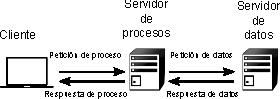
\includegraphics[width=0.75\textwidth]{Cliente_servidor/Datos_y_procesos_remotos.pdf}
\caption{\small Esquema de acceso a un servicio de procesos remotos, el cual a su vez utiliza datos de un segundo servidor. El encadenamiento de procesos permite ampliar notablemente la utilidad de estos.}
\label{Fig:Datos_y_procesos_remotos} 
\end{figure}

\end{itemize}

\subsection{Clientes}

\index{Cliente}
El cliente es el elemento que utiliza los datos proporcionados por el servicio. Para ello, realiza una petici�n a la que el servicio responde enviando dichos datos, que ser�n los que despu�s se emplear�n para realizar cualquier otra tarea, principalmente la representaci�n de estos para que el usuario pueda visualizarlos. El cliente es, de este modo, el intermediario entre el usuario y los servicios y datos que el servidor ofrece.

Como hemos visto al estudiar los servidores, las principales capacidades de estos implican la transmisi�n de im�genes con cartograf�a ya elaborada, o bien directamente capas, ya sean de tipo r�ster o vectoriales. En algunos casos, el servicio ofrecido es un servicio de procesos, pero su resultado generalmente es tambi�n una capa, por lo que, desde el punto de vista del cliente, la funcionalidad es en cierto modo similar (aunque internamente requiera una implementaci�n por completo distinta).

El cliente, por tanto, debe disponer de capacidades para formular peticiones a servidores como los anteriormente descritos, as� como para emplear las posibles respuestas que estos devolver�n. Estas �ltimas incluyen por lo general componentes de representaci�n, habitualmente con la forma t�pica de un visor en el que se permite cambiar la escala y desplazar la vista, tal y como ya vimos en el cap�tulo \ref{SIGs_escritorio}. No obstante, estas capacidades pueden variar ampliamente de un cliente a otro, desde el m�nimo necesario para simplemente representar los datos obtenidos del servidor hasta conjuntos de funcionalidades mucho m�s avanzadas pensadas para un uso intensivo de esos mismos datos.

Distinguimos as� dos tipos de clientes en funci�n de las capacidades que tengan: \emph{clientes ligeros} y \emph{clientes pesados}.

\begin{itemize}
	\item \textbf{Cliente ligero}. Se denomina \emph{ligero} por el tama�o relativamente reducido del programa en s�, lo cual va consecuentemente asociado a unas capacidades limitadas. Hablamos de clientes ligeros cuando nos referimos a \emph{Web Mapping} y a clientes que se ejecutan sobre un navegador Web, los cuales son siempre sencillos en cuanto a sus funcionalidades. En el momento de la carga de la p�gina Web que contiene al cliente, el navegador descarga toda la l�gica del programa, lo cual hace necesario limitar el tama�o de este.
	
	No obstante, los clientes Web empiezan progresivamente a ampliar sus posibilidades, y en ello juegan un importante papel otros servicios distintos a los de mapas o los de datos, como pueden ser los de procesos. Estos permiten que las funcionalidades adicionales no se implementen en el propio cliente (y por tanto sin aumentar en exceso su tama�o y sin disminuir su <<ligereza>>), sino que sean accedidas tambi�n como servicios remotos.
	
	La evoluci�n de la cartograf�a Web en esta direcci�n se dirige desde el \emph{Web Mapping} al \emph{Web GIS}, tal y como comentamos algunas p�ginas atr�s.





		Adem�s de modificar la zona representada, un usuario debe poder modificar la forma en que los datos dentro de esa zona se muestran. Es decir, debe poder cambiar el estilo de los elementos representados, variando colores o formas de la misma manera que esto puede hacerse en un SIG de escritorio. Asimismo, muchas aplicaciones Web permiten la consulta de varias capas de datos, incluso de datos provenientes de varios servidores distintos, datos que no necesariamente han de mostrarse todos simult�neamente. Igual que en un SIG de escritorio seleccionamos unas u otras capas para su visualizaci�n y podemos alterar el orden de representaci�n de estas, tambi�n podemos realizar estas operaciones en una aplicaci�n SIG Web.

		Esto hace que una aplicaci�n SIG dentro de un navegador se convierta en una herramienta completa para el acceso a uno o varios juegos de datos remotos cuyo contenido es abundante (no solo en extensi�n sino tambi�n en tipos de datos suministrados), ya que permite una gran configurabilidad y deja en manos del cliente (esto es, del usuario), la forma de tomar esos datos y mostrarlos.

		Las capacidades de edici�n tambi�n tienen lugar en los SIG Web, ampliando las posibilidades que la interactividad m�s b�sica ofrece. Un usuario puede a�adir su propia informaci�n a un SIG Web o bien modificar una capa existente empleando su navegador. Las tecnolog�as SIG siguen en este sentido a las tecnolog�as Web m�s generales, adoptando los conceptos de la Web 2.0 y ampliando las posibilidades de los usuarios de colaborar directamente en los contenidos de la red. Por ejemplo, \emph{OpenStreetMap} \cite{webOSM} es un sitio equivalente a la bien conocida Wikipedia, en el cual los usuarios pueden a�adir sus propias descripciones de elementos geogr�ficos que ellos mismos definen.\index{Wikipedia}\index{OpenStreetMap}

		A estas mismas tecnolog�as se les puede dar usos m�s restringidos sin que necesariamente sea dentro de un proyecto colaborativo abierto. Por ejemplo, una administraci�n local puede dar acceso a los propietarios de suelo para que puedan consultar su catastro, mediante un sistema de autenticaci�n conveniente, incluso editar informaci�n de sus parcelas. Est� informaci�n puede ser de tipo no espacial (es decir, los l�mites de las parcelas ser�an fijos), ya que las capacidades de edici�n no han de limitarse a la componente espacial.\index{Autenticaci�n}

		Por �ltimo, y aunque en la actualidad son pocos los servicios de este tipo que existen, y no pueden compararse las prestaciones con las que ofrecen los SIG de escritorio, la cartograf�a Web puede ofrecer herramientas de an�lisis. Adem�s de representar un conjunto de datos geogr�ficos y permitir al usuario navegar en ellos e incluso editarlos, pueden extraerse resultados a partir de esos datos. 

		Un tipo de aplicaci�n bastante extendida de este tipo es el c�lculo de rutas �ptimas. A partir de una capa con v�as de comunicaci�n un usuario establece un punto de salida y otro de destino y la aplicaci�n Web calcula la ruta que optimiza el tiempo empleado o la distancia total recorrida, seg�n lo explicado en el cap�tulo \ref{Costes}. \cite{webGuiaCampsa} es un ejemplo de este tipo de aplicaciones en el cual la interfaz no es la de un SIG de escritorio habitual, sino que se introducen los lugares de origen y destino tecleando sus nombres y despu�s la ruta calculada se muestra sobre un mapa y tambi�n como un conjunto de indicaciones a seguir. Es decir, que sobre una base de c�lculo SIG se crea una aplicaci�n m�s completa que la que es habitual encontrar en un SIG, aprovechando la mayor riqueza de elementos que pueden utilizarse dentro de un navegador Web.

		El t�rmino \emph{Web Mapping}, habitualmente empleado para designar a la cartograf�a Web, se sustituye por \emph{Web GIS} a medida que las capacidades de las aplicaciones Web aumentan, para indicar as� que todos los componentes que forman parte de un SIG en su sentido cl�sico, esto es, un SIG de escritorio, se incorporan a dicha aplicaci�n Web.\index{Web GIS}




	
	\item \textbf{Cliente pesado}. A diferencia del cliente ligero, el cliente \emph{pesado} es una aplicaci�n individual que no se ejecuta sobre otra aplicaci�n soporte como puede ser un navegador Web. Al ser un programa independiente, debe ocuparse de toda la l�gica del proceso y de proveer todas las funcionalidades necesarias, por lo que su tama�o es generalmente mayor. Pese a ello, un cliente pesado no ha de ser necesariamente m�s potente y con m�s funcionalidades que uno ligero (aunque habitualmente lo es), ya que existen aplicaciones muy sencillas con capacidad para conectarse a servicios de mapas, que ofrecen poco m�s que un visor de cartograf�a. La diferencia no estriba en las capacidades del programa, sino en el enfoque a la hora de implementar este y el uso o no de otra aplicaci�n <<plataforma>>, generalmente en forma de un navegador Web.
	
	Los clientes pesados suelen permitir el uso de datos no procedentes directamente del acceso a servicios, tales como datos en ficheros locales, y no est�n pensados exclusivamente como clientes, sino como aplicaciones m�s amplias que adem�s disponen de capacidades para aprovechar un determinado tipo de servicios. Dicho de otro modo, un cliente pesado tal y como un SIG de escritorio tiene utilidad aunque no se emplee como cliente de ning�n servicio y no se disponga de conexi�n a red alguna, ya que puede alimentarse con datos locales y todas sus restantes funcionalidades (an�lisis, preparaci�n de cartograf�a, etc.) pueden aprovecharse con dichos datos.
\end{itemize}

\index{Cliente!ligero}\index{Cliente!pesado}

\section{Limitaciones y problemas de la cartograf�a Web}

Trasladar las ideas de los SIG de escritorio a la Web no es sencillo, por cuanto el entorno en el que nos movemos es muy distinto en uno y otro caso. La Web tiene sus propias limitaciones e inconvenientes, que en muchos casos no existen en el caso de una aplicaci�n de escritorio, y este hecho presenta dificultades complejas de salvar, obligando a desarrollar soluciones alternativas.

Una limitaci�n b�sica es la impuesta por el propio navegador como marco de trabajo. Las propias ventajas que este aporta son tambi�n responsables de ciertas limitaciones, ya que en el desarrollo de una aplicaci�n SIG Web no se tiene la misma libertad que al desarrollar una aplicaci�n de escritorio. Este no es un problema exclusivo del \emph{Web Mapping}, sino en general de todas las aplicaciones Web, que, pese a los avances que han tenido lugar en este sentido y la r�pido evoluci�n de las tecnolog�as Web, siguen sin poder ofrecer exactamente las mismas funcionalidades en lo que a interfaces respecta. 


A lo anterior debemos sumar el hecho de que las tecnolog�as Web en general son recientes y en cierto modo inmaduras, y aunque se emplea gran cantidad de medios y esfuerzo en el �mbito Web debido a su vital importancia en la actualidad, una buena parte de los elementos tecnol�gicos sobre los que se fundamenta el \emph{Web Mapping} actual no est�n todav�a completamente desarrollados y necesitan a�n evolucionar.

El aspecto m�s problem�tico es, no obstante, la propia red, especialmente en lo que respecta a su fiabilidad y rendimiento. Todos los datos que el cliente emplea en una aplicaci�n de cartograf�a Web provienen de la red, y por tanto existe una fuerte dependencia entre la aplicaci�n y el funcionamiento tanto de esta como del servidor que a trav�s de ella nos proporciona esos datos.

Si abrimos un archivo con datos espaciales en nuestro ordenador desde un SIG de escritorio, podemos casi garantizar que esa misma operaci�n funcionar� de igual modo si la repetimos en otro momento. Tener esa misma seguridad cuando se trabaja con datos remotos no es tan sencillo, ya que la red puede no funcionar o el servidor puede estar recibiendo en este momento gran cantidad de peticiones de otros clientes y no ser capaz de gestionarlas eficientemente y ofrecernos al instante respuesta a nuestra petici�n. En definitiva, las mismas circunstancias que afectan a todas las aplicaciones Web y que son conocidas por todos.

El rendimiento de la red es m�s importante a�n si cabe en el caso de trabajar con informaci�n geogr�fica, ya que los datos suelen ser voluminosos. Visualizar un mapa y que este pueda desplazarse y modificarse de forma igual de fluida que al trabajar con una aplicaci�n de escritorio requiere por un lado un ancho de banda suficiente para transmitir la gran cantidad de datos necesarios, y por otro la implementaci�n de algunas t�cnicas particulares que facilitan este proceso. Por su importancia, veremos en detalle las t�cnicas de \emph{tiling} (divisi�n horizontal de los datos geogr�ficos en teselas) y \emph{cacheo} (almacenamiento temporal de datos en la m�quina del cliente), utilizadas habitualmente en la actualidad.

\subsection{\emph{Tiling} y \emph{cacheo}}

\index{Tiling}\index{Cacheo}

Dos t�cnicas b�sicas que se emplean actualmente en los clientes Web que manejan informaci�n geogr�fica son el \emph{tiling} y el \emph{cacheo}. Estas t�cnicas permiten que la experiencia de trabajar con informaci�n geogr�fica dentro de una aplicaci�n SIG Web sea m�s agradable, logrando una mayor fluidez y superando en cierta medida las limitaciones de la red. Aunque es cierto que cada vez disfrutamos de mayores anchos de banda y velocidades de transmisi�n m�s altas, tambi�n aumentan de igual modo los vol�menes de datos manejados, con lo que las dificultades siguen existiendo de manera similar.

Ambas t�cnicas se utilizan en servicios en los que el servidor provee im�genes, ya que es en estos en los que resultan aplicables, y tambi�n donde es m�s necesario recurrir a este tipo de t�cnicas.

El \emph{tiling} es una t�cnica consistente en dividir las im�genes con las que se trabaja en im�genes menores que formen un mosaico. Esto permite un trabajo m�s r�pido, al utilizar unidades m�nimas de menor tama�o y poder reducir la necesidad de transmitir datos a trav�s de la red si se realiza una gesti�n correcta del conjunto de elementos de ese mosaico.

Esta divisi�n es similar en forma a la propia que se da en los datos originales, ya que, como sabemos (v�ase secci�n \ref{divisionHorizontal}), estos tambi�n se encuentran divididos horizontalmente. No obstante, se trata de una estrategia propia del sistema cliente--servidor, que divide las propias im�genes que luego se representar�n en este �ltimo, de forma que en lugar de transmitir una �nica imagen se transmiten varias de menor tama�o y la informaci�n correspondiente a la posici�n relativa de estas.

El \emph{cacheo}, por su parte, es una t�cnica no exclusiva del �mbito SIG, sino de la Web en general, y consiste en almacenar de forma temporal los datos obtenidos de un servidor en la m�quina local o bien en una m�quina intermedia (\emph{proxy}\index{Proxy}). De este modo, si volviera a resultar necesario acceder a esos datos, no han de pedirse al servidor, sino que pueden recuperarse de la copia local, con las ventajas que ello tiene en cuanto a la velocidad de acceso y la fiabilidad del proceso.

El uso conjunto de \emph{tiling} y \emph{cacheo} puede disminuir sensiblemente el volumen de datos a transmitir para, por ejemplo, modificar el encuadre de un mapa en una aplicaci�n SIG Web. La figura \ref{Fig:Tiling} muestra un ejemplo sencillo que servir� para comprender el ahorro de datos que puede conseguirse con el uso conjunto de estas t�cnicas.

\begin{figure}[!hbt]   
\centering
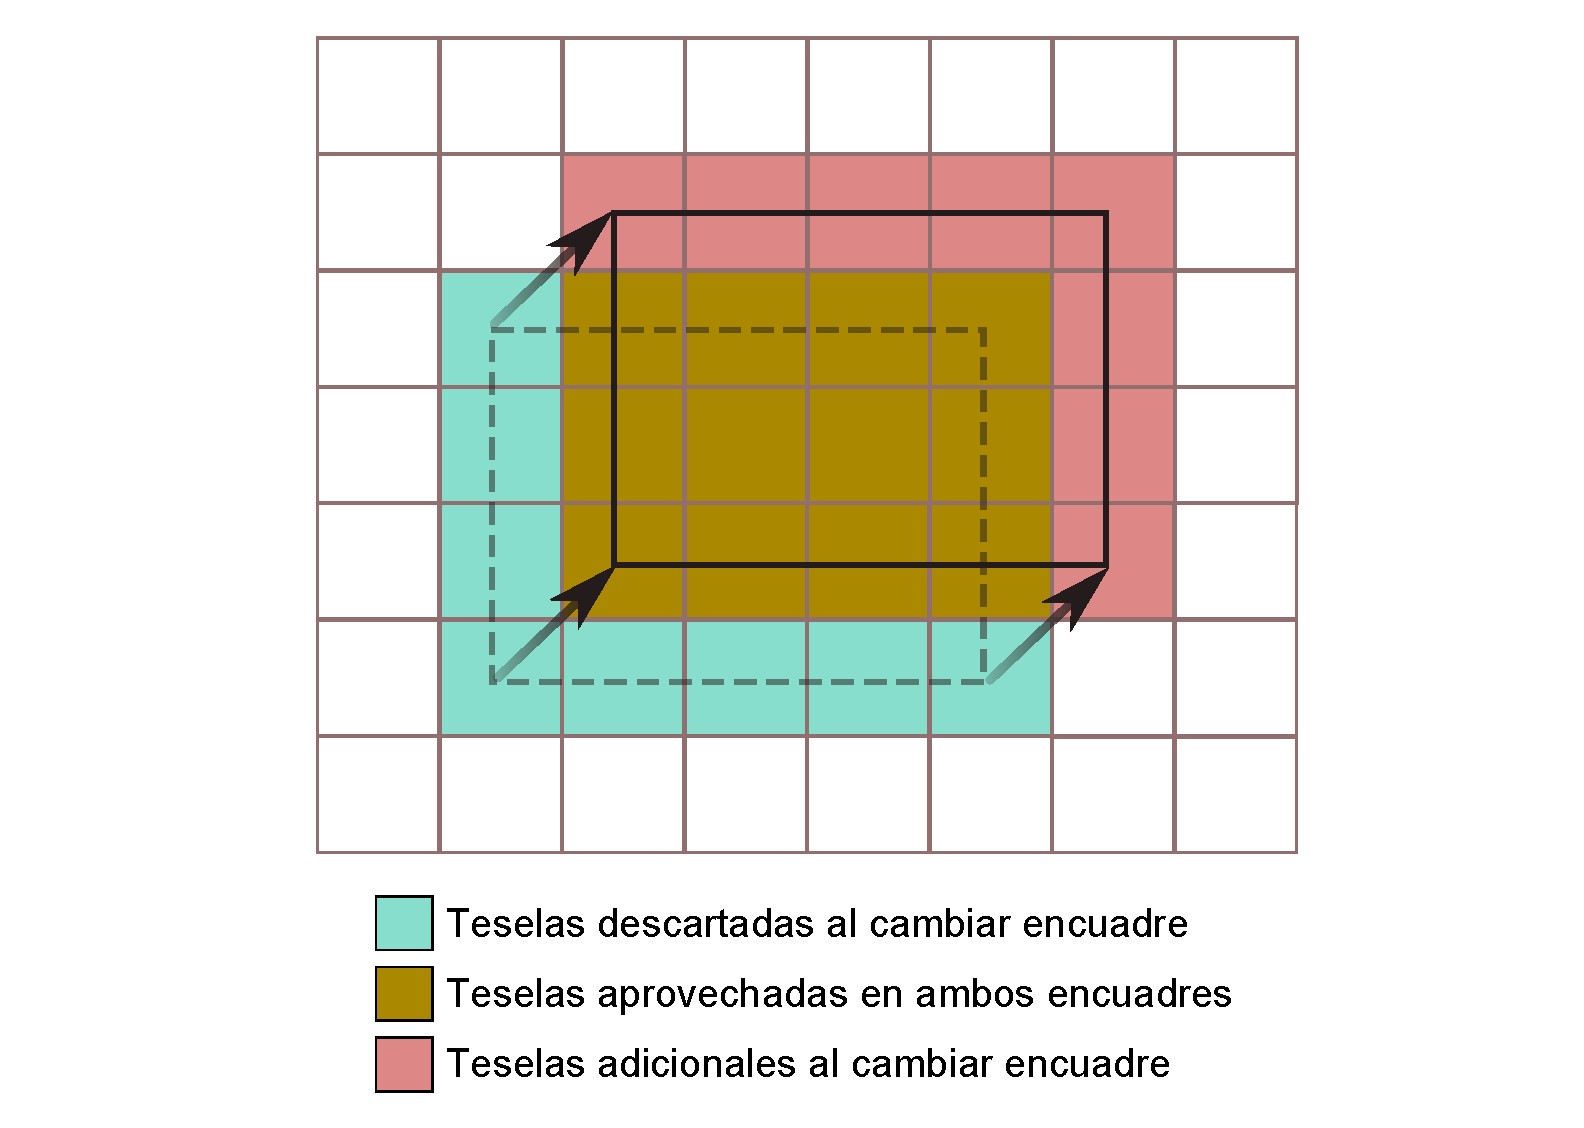
\includegraphics[width=.8\textwidth]{Cliente_servidor/Tiling.pdf}
\caption{\small Esquema del uso de \emph{tiling} y \emph{cacheo} para optimizar la transmisi�n de datos en una aplicaci�n SIG Web}
\label{Fig:Tiling} 
\end{figure}

En la figura puede verse del dato global al que se accede, dividido en una serie de unidades. Ello no quiere decir que el dato tenga ese n�mero de divisiones o que existan otros tantos ficheros. Puede tratarse de un �nico fichero, o de un n�mero muy elevado de ellos. Las divisiones se realizan a efectos de crear el mosaico de im�genes a la hora de transmitir estas.

Inicialmente, la aplicaci�n Web encuadra una regi�n que cubre 20 elementos o teselas. Si el usuario desplaza el encuadre para que cubra otro �rea distinta, como en el caso mostrado en la figura, el cliente realizar� una nueva petici�n y obtendr� una nueva imagen, que tendr� exactamente el tama�o con que esa imagen va a representarse. Este es exactamente el mismo tama�o que la imagen que encontramos inicialmente en el encuadre original, y por tanto la representaci�n de este encuadre original y posteriormente el encuadre modificado requiere transmitir dos im�genes que cubren cada una de ellas veinte teselas.

Si, por el contrario, aplicamos conjuntamente las t�cnicas anteriores de \emph{tiling} y \emph{cacheo}, al variar el encuadre no es necesario obtener del servidor una imagen que cubra todo el �rea a representar, sino tan solo los 8 elementos correspondientes a la zona no cubierta por la imagen inicial, ya que los restantes ya habr�n sido obtenidos con anterioridad y se encontrar�n almacenados (\emph{cacheados}) en nuestro ordenador. Es decir, el cliente crea la imagen a representar con 8 subimagenes pedidas al servidor y otras 12 ya descargadas previamente, reduciendo sensiblemente el volumen de datos pedidos al servidor.

Cuando este esquema de funcionamiento se combina con tecnolog�as como AJAX, citada anteriormente, y que a�ade a su vez mayor fluidez y una mejor respuesta de la aplicaci�n Web, el resultado es una aplicaci�n SIG altamente funcional y cuyo comportamiento se asemeja en cuanto a rendimiento al de un SIG de escritorio trabajando con datos locales.\index{AJAX}

Este tipo de t�cnicas no son exclusivas de los SIG en Internet, sino que tambi�n se aplican por igual al caso de SIG de escritorio cuando estos act�an como clientes y acceden a datos remotos. Particularmente, son de especial relevancia en el caso de los globos tridimensionales, en los cuales estas mismas t�cnicas se aplican no solo para las im�genes a visualizar, sino tambi�n para los datos de elevaci�n empleados para dar forma al relieve.

La combinaci�n de \emph{tiling} y \emph{cacheo} se lleva a cabo a m�ltiples escalas, de forma que se reduce el n�mero de operaciones a realizar y se obtiene un mayor rendimiento. Se emplean las denominadas \emph{pir�mides}, que ya vimos en el apartado \ref{Generalizacion_en_SIG} dedicado a la generalizaci�n cartogr�fica en un SIG. Estas pueden ser empleadas tambi�n en el lado del servidor, incluso cuando este sirve mapas creados a partir de cartograf�a vectorial. Para evitar tener que rasterizar los datos vectoriales cada vez que se realiza una petici�n (lo cual supondr�a un gran coste en t�rminos de proceso), se rasterizan de antemano a distintas escalas, de forma que cuando el cliente efect�a la petici�n ya se dispone de una imagen que servirle, sea cual sea la escala que pida.\index{Pir�mides}.

Una t�cnica de reciente aparici�n es la denominada emph{tiling vectorial}. Aplicando los mismos principios que el \emph{tiling}, es decir, la subdivision de los datos de forma regular, las capas vectoriales se <<trocean>> en el origen y se env�an despu�s solamente los datos necesarios para el area cubierta en el cliente. Combinando este enfoque con el uso de capas con distinto detalle seg�n la escala, se logran dos ventajas: 

\begin{itemize}
\item Disminuci�n del volumen de datos. 
\item Capacidad de modificar la simbolog�a en el cliente.
\end{itemize}

Al enviar los datos en lugar de una representaci�n de estos, el cliente es quien debe establecer la simbolog�a, lo cual permite que sea el usuario quien seleccione c�mo representar los elementos vectoriales. Al mismo tiempo, se logran ventajas en la experiencia de usuario, debidas principalmente a la escalabilidad de los datos vectoriales, que permite por ejemplo presentar transiciones m�s fluidas cuando se modifica la escala del mapa.

Obviamente, este tipo de enfoque es v�lido unicamente para el caso de capas vectoriales.



\section{Est�ndares}

Para garantizar el buen funcionamiento de un sistema cliente--servidor, es importante definir de forma adecuada c�mo se establece la comunicaci�n entre clientes y servidores, de forma que estos primeros no solo puedan obtener los propios datos geogr�ficos de estos �ltimos, sino tambi�n realizar consultas o conocer qu� otras funcionalidades se encuentran disponibles.

En otras palabras, resulta necesario definir una \emph{lingua franca} para que todas las comunicaciones se produzcan de forma fluida. Esto obliga a establecer una cierta normalizaci�n y crear elementos estandarizados que sean conocidos e implementados por las distintas partes, y hacerlo para cada uno de los servicios ofrecidos, as� como para los propios datos. Esta \emph{lingua franca} es lo que denominamos un \emph{Est�ndar}.

El modelo de cliente--servidor en t�rminos tecnol�gicos no es muy diferente de la idea de un cliente y un proveedor de servicios en la vida real. Una persona (el cliente) que quiera adquirir un producto de un distribuidor (el servidor) debe igualmente comunicarse con �l para preguntarle si dispone del producto deseado, realizar una petici�n de este y despu�s recibirlo cuando el distribuidor se lo env�e. Por ejemplo, un usuario puede consultar el cat�logo para localizar un dato concreto y despu�s acceder a �l remotamente mediante, por ejemplo, un cliente Web. Ambos esquemas de funcionamiento son muy semejantes.

Imaginemos ahora la situaci�n en la que una persona en Espa�a desea adquirir un producto electr�nico de un proveedor chino. En primer lugar, es probable que tenga dificultades para entender el cat�logo de productos, pues este describir� cada uno de ellos en chino. Si consigue localizarlo y desea adquirirlo, es igualmente probable que encuentre dificultades para comunic�rselo al proveedor, ya que seguir� existiendo la misma barrera ling��stica. Y si finalmente recibe el producto, puede tener dificultades al utilizarlo, ya que este puede funcionar a un voltaje distinto al de la red el�ctrica espa�ola o bien estar preparado para un tipo de enchufe distinto. 

Este peque�o ejemplo nos hace ver que en la relaci�n cliente--servidor pueden surgir problemas derivados de la falta de elementos comunes entre ambos actores. Si todos los elementos que toman parte en el establecimiento de esa relaci�n comercial estuvieran normalizados y fueran �nicos, un comprador de cualquier parte del mundo podr�a de forma inmediata comprar un dispositivo a cualquier vendedor de otro pa�s comunic�ndose en un �nico idioma, y tener despu�s la garant�a de poder usarlo sin problemas.

En el �mbito de la informaci�n geogr�fica la situaci�n es similar a la anterior. Hay muchos formatos distintos para almacenarla y muchas formas distintas de transmitirla, y ello dificulta el trabajo. Igual que los clientes espa�oles no hablan el mismo idioma que los vendedores chinos, no todos los clientes SIG hablan el mismo idioma que todos los servidores, y dos cualesquiera de ellos no han de <<entenderse>> necesariamente.

De hecho, hist�ricamente los distintos fabricantes de clientes defin�an por s� mismos la forma en que sus programas se comunicaban, que no coincid�a con la del resto de fabricantes. Un cliente de un fabricante dado no podr�a acceder a los servicios de un servidor creado por un fabricante distinto. Este paradigma, caracter�stico del software privativo, es un problema, pues dificulta el acceso a los datos.

En circunstancias ideales, debe existir una total \emph{interoperabilidad} con independencia de los formatos y las aplicaciones empleadas, pudiendo interactuar entre s� los distintos clientes y servidores. Los est�ndares son el elemento que va a permitir esa interoperabilidad, definiendo el marco com�n que clientes y servidores emplear�n para entenderse. En un contexto altamente heterog�neo tanto en datos como en herramientas, lograr esto no resulta una tarea sencilla\cite{Lemmenes2006IEEE}, y los est�ndares son los encargados de aportar homogeneidad tecnol�gica.

\subsection{Est�ndares abiertos e interoperabilidad}

La interoperabilidad implica que podemos sustituir unos elementos del sistema en el que se incluyen los clientes y servidores por otros distintos, teniendo la seguridad de que van a interaccionar entre ellos sin dificultades. Las funcionalidades que un cliente o servidor nos ofrece pueden ser distintas a las de otro, pero independientemente de su origen (independientemente del fabricante), si esos elementos implementan un est�ndar dado, siempre podr�n interactuar con todos aquellos que tambi�n lo implementen.

La clave, por tanto, est� en los est�ndares, y en particular en que estos sean est�ndares \emph{abiertos}. Un est�ndar es un documento o pr�ctica que busca armonizar los aspectos t�cnicos de un producto o servicio. 

Un est�ndar se considera como tal cuando es empleado por un grupo o comunidad, que lo acepta para la definici�n de las caracter�sticas de ese producto o servicio en su seno. Si �nicamente es el uso del est�ndar el que lo ratifica como tal, se denomina est�ndar \emph{de facto}. El formato \emph{shapefile} para capas vectoriales, por ejemplo, es uno de estos est�ndares, ya que est� ampliamente difundido y existe tal cantidad de datos en este formato que todas las aplicaciones deben implementarlo para tener valor pr�ctico.\index{Shapefile}

Existen est�ndares que se convierten en normas o est�ndares \emph{de iure}, cuando estos son promovidos por alg�n organismo oficial de normalizaci�n o su uso se impone con car�cter legal. 

Un est�ndar \emph{abierto} es aquel cuya definici�n se encuentra disponible y todo aquel que lo desee puede conocerla y emplearla para el desarrollo de la actividad relacionada con ese est�ndar. En nuestro campo de trabajo, eso quiere decir que cualquier desarrollador que desee crear un nuevo cliente o servidor para datos SIG puede acceder al est�ndar y desarrollar en base a este.

Los principios fundamentales de los est�ndares abiertos son los siguientes \cite{perensEstandares}:

\begin{itemize}
	\item \textbf{Disponibilidad}. Los est�ndares abiertos est�n disponibles para todos el mundo para su lectura y uso en cualquier implementaci�n.
	\item \textbf{M�xima posibilidad de elecci�n para los usuarios finales}. Los est�ndares abiertos crean un mercado competitivo y justo, y no bloquean a los usuarios en el entorno de un vendedor particular. Desde el punto de quienes venden la tecnolog�a SIG, esto no es tan ventajoso, ya que permite la aparici�n de competidores que antes no pod�an existir. Si un fabricante basa sus productos en un est�ndar cerrado definido por �l mismo, otros no pueden elaborar soluciones que trabajen con esos productos, ya que no conocen el est�ndar empleado. 
	
	Asimismo, el fabricante puede cambiar el est�ndar utilizado por, por ejemplo, su producto de servidor, y obligar a los consumidores y a todo aquel que quiera utilizar un servicio basado en ese servidor a que actualicen tambi�n los clientes, pues los anteriores ya no podr�n comunicarse con el nuevo servidor. Utilizando est�ndares abiertos, la competencia entre fabricantes ha de basarse puramente en las capacidades que ofrecen, con lo que los consumidores ganan en calidad de los productos y en posibilidades de elecci�n.
	\item \textbf{Gratuidad}. Implementar un est�ndar es gratuito, sin necesidad de pagar, como en el caso de una patente. Los organismos que generan los est�ndares pueden cobrar una cierta cantidad por acceder a la definici�n de los est�ndares, con objeto de financiar as� la labor que desarrollan, y tambi�n pueden cobrar por emitir certificados de que un determinado producto o servicio se ha desarrollado de acuerdo con el est�ndar.
	\item \textbf{Discriminaci�n}. Los est�ndares abiertos y las organizaciones que los desarrollan no favorecen de ning�n modo a uno u otro implementador sobre los restantes.
	
	\item \textbf{Extensi�n o creaci�n de subconjuntos de un est�ndar}. Los est�ndares abiertos pueden ser extendidos o bien presentados como subconjuntos del est�ndar original.
	\item \textbf{Pr�cticas predatorias}. Los est�ndares abiertos pueden tener licencias que requieran a todo aquel que desarrolle una extensi�n de dicho est�ndar la publicaci�n de informaci�n acerca de esa extensi�n, y el establecimiento de una licencia dada para todos aquellos que creen, distribuyan y vendan \emph{software} compatible con ella. Un est�ndar abierto no puede prohibir de otro modo el desarrollo de extensiones.
\end{itemize}

Para tener una noci�n de lo que en la pr�ctica realmente significa el uso de est�ndares abiertos en el campo de los SIG, podemos ver la figura \ref{Fig:Esquema_no_interoperable}, donde se representa el esquema de una arquitectura no interoperable. Es decir, una arquitectura que no se basa en este tipo de est�ndares.

\begin{figure}[!hbt]   
\centering
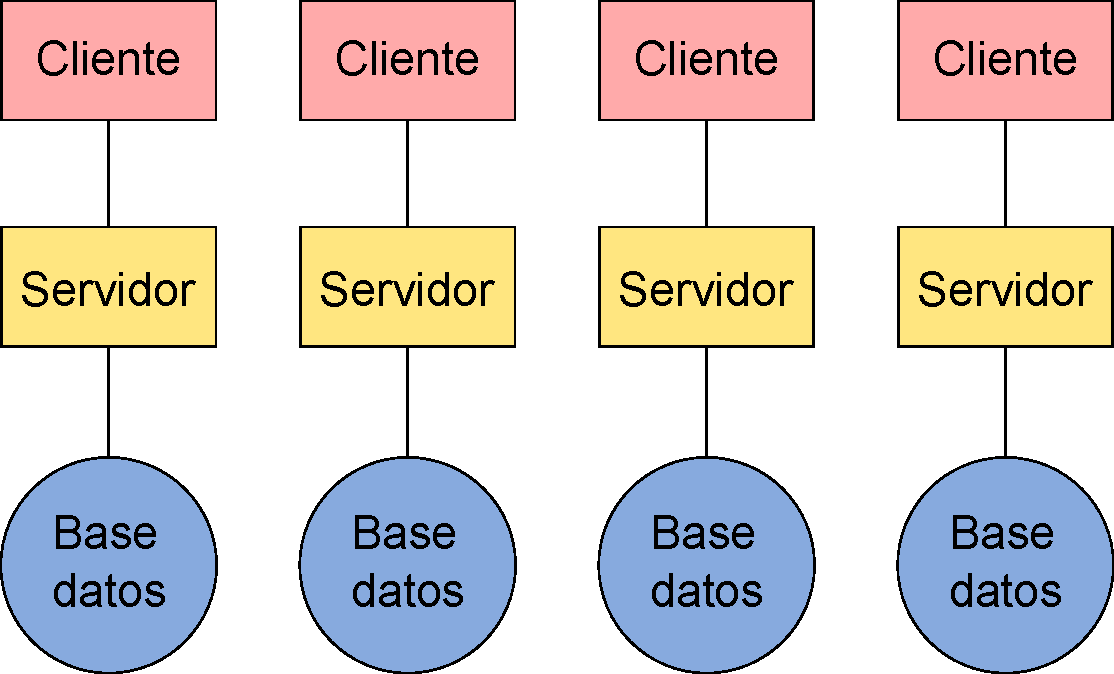
\includegraphics[width=.5\mycolumnwidth]{Cliente_servidor/Esquema_no_interoperable.pdf}
\caption{\small Esquema de una arquitectura no interoperable.}
\label{Fig:Esquema_no_interoperable} 
\end{figure}

Los datos que se encuentran en cada base de datos son accesibles �nicamente a trav�s de un �nico cliente, que es aquel correspondiente al servidor que ofrece servicios basados en esos datos. Los restantes datos quedan fuera del alcance de ese cliente, ya que no es capaz de acceder a ellos. Las diferentes soluciones cliente--servidor crean en esta situaci�n un conjunto de islas tecnol�gicas, cada una completamente independiente y sin posibilidad alguna de interactuar con las restantes.

Entre los principales inconvenientes de una arquitectura no interoperable como la representada podemos citar los siguientes:

\begin{itemize}
\item \textbf{ Desperdicio de recursos}. Cada servicio debe gestionar sus propio conjunto de datos, lo cual requiere abundantes recursos y no es sencillo, adem�s de implicar un elevado coste.
\item \textbf{ Necesidad de conocer m�ltiples clientes}. Si para acceder a cada servicio necesitamos su cliente particular, acceder al conjunto de servicios ofrecidos por esos servidores requiere por parte de los usuarios aprender a utilizar tantos clientes como servidores existan.
\item \textbf{ Imposibilidad de combinar datos}. Dos datos a los que pueda accederse a trav�s de dos servidores distintos no podr�n utilizarse simult�neamente en un �nico cliente, ya que este no podr� comunicarse con ambos servidores. Un an�lisis que requiera distintos tipos de datos no podr� realizarse si todos ellos no se ofrecen a trav�s de un mismo servidor.
\item \textbf{Imposibilidad de combinar funcionalidades}. Los datos ofrecidos por un servidor pueden usarse para el desarrollo de muchas tareas. Estas tareas requieren que las correspondientes herramientas est�n disponibles en los clientes, y estos se diferencian notablemente, de la misma forma que lo hacen tambi�n los SIG de escritorio entre s�. Si acceder a los datos a trav�s de un servidor solo se puede hacer empleando un cliente concreto, no existe la posibilidad de aprovechar las funcionalidades de otro cliente sobre esos mismos datos, y el usuario ve as� limitadas sus posibilidades de trabajo.
\end{itemize}

En contraste con lo anterior, tenemos una situaci�n de plena interoperabilidad basada en est�ndares abiertos como la representada en el esquema de la figura \ref{Fig:Esquema_interoperable}.

\begin{figure}[!hbt]   
\centering
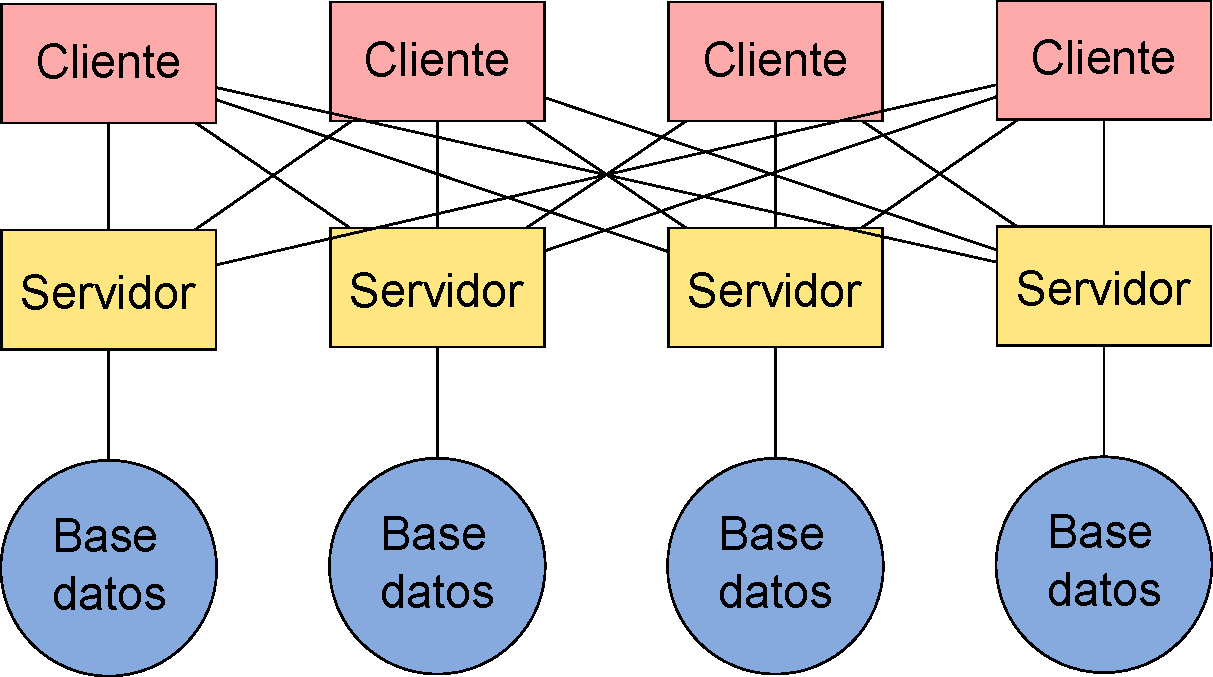
\includegraphics[width=.5\mycolumnwidth]{Cliente_servidor/Esquema_interoperable.pdf}
\caption{\small Esquema de una arquitectura interoperable.}
\label{Fig:Esquema_interoperable} 
\end{figure}

En este caso, existe un servidor que es el que gestiona y ofrece los servicios para cada base de datos, pero a �l pueden acceder todos los clientes, ya que por el hecho de estar basados en est�ndares abiertos es posible una comunicaci�n plena entre dos cualesquiera de ellos.

En esta situaci�n, un usuario puede emplear su cliente favorito (siempre que este implemente los est�ndares pertinentes) para acceder a muchos servicios distintos, o bien puede utilizar varios clientes para acceder a unos mismos datos, eligiendo en cada momento el que m�s le convenga seg�n sus necesidades. Las posibilidades de trabajo se multiplican cuando la arquitectura del sistema se fundamenta en est�ndares abiertos.

Las ventajas no son solo para los usuarios, sino tambi�n para los desarrolladores. A la hora de crear un cliente, no es necesario comprobar que este se comunica bien con todos los servidores y funciona correctamente, sino simplemente seguir las especificaciones del est�ndar. Todo aquel servidor que las implemente funcionar� sin dificultades, ya que el est�ndar garantiza la buena comunicaci�n y la interoperabilidad.

\subsection{Entidades creadoras de est�ndares}

Crear un est�ndar no es una labor sencilla. Se han de recoger las principales necesidades y armonizar todas ellas en una especificaci�n �nica, de modo que clientes y servidores que implementen ese est�ndar sean de la mayor utilidad posible para todos los usuarios.

Existen organizaciones dedicadas a redactar las especificaciones correspondientes a est�ndares que cubran los distintos servicios, as� como a promoverlas y mejorarlas. Los est�ndares m�s habituales en el campo de la informaci�n geogr�fica son elaborados por tres organizaciones: el Open Geospatial Consortium (OGC), ISO y W3C.

\subsubsection{Open Geospatial Consortium (OGC)}

El Open Geospatial Consortium \cite{webOGC} es una organizaci�n internacional y voluntaria dedicada a la elaboraci�n de est�ndares. En el OGC participan m�s de 350 organizaciones miembro, incluyendo entre ellas a los principales fabricantes del sector, agencias nacionales, grupos de investigaci�n u organizaciones sin �nimo de lucro, entre otros. Estas organizaciones miembro colaboran para alcanzar consensos y desarrollar e implementar est�ndares en el �mbito de los contenidos geoespaciales.

Algunos de los est�ndares OGC m�s relevantes, los cuales veremos a lo largo de este cap�tulo, son los siguientes:

\begin{itemize}
\item \textbf{ WMS}. Para obtener im�genes de mapas.
\item \textbf{ WCS}. Para obtener y consultar coberturas.
\item \textbf{ WFS}. Para obtener y editar entidades geogr�ficas y sus atributos asociados.
\item \textbf{ WPS}. Para servicios de procesos remotos.
\item \textbf{ GML}. Para almacenamiento de informaci�n geogr�fica.
\item \textbf{ CSW}. Para consultas en cat�logos.
\end{itemize}

Cada uno de estos est�ndares est� descrito en una especificaci�n, y estas est�n sujetas a cambios y mejoras, existiendo varias versiones en cada caso. 

\subsubsection{ISO}

ISO \cite{webISO} es una organizaci�n internacional dedicada a la elaboraci�n de est�ndares no solo en el �mbito geogr�fico, sino en todas las �reas. ISO es responsable, por ejemplo, de est�ndares bien conocidos y aplicados en la industria actual, tales como los relacionados con la gesti�n medioambiental en empresas o los est�ndares de calidad.

Dentro de ISO existen diversos comit�s t�cnicos, cada uno de los cuales se encarga de definir los est�ndares correspondientes a un campo de trabajo. El comit� ISO/TC 211 es el responsable de aquellos relacionados con la informaci�n geogr�fica digital.

ISO redacta Especificaciones T�cnicas y Est�ndares Internacionales, catalogando estos con un n�mero que los identifica. Los elaborados por ISO/TC 211 corresponde a la serie 19100.

Existe una estrecha relaci�n entre ISO y OGC, y los est�ndares elaborados por ambas organizaciones son muchos de ellos muy similares o incluso id�nticos. De hecho, algunos de los est�ndares desarrollados por el OGC, como WMS o GML, citados anteriormente y que en breve detallaremos, son tambi�n est�ndares ISO.

En \cite{webDocsISOTC211} puede consultarse la lista de normas ISO/TC211 aprobadas y el estado de cada uno de sus documentos de trabajo.

\subsubsection{W3C}

El Consorcio World Wide Web (W3C) es un consorcio internacional donde las organizaciones miembro, personal a tiempo completo y el p�blico en general, trabajan conjuntamente para desarrollar est�ndares Web. Seg�n su propia definici�n\cite{webW3C}, la misi�n del W3C es <<guiar la Web hacia su m�ximo potencial a trav�s del desarrollo de protocolos y pautas que aseguren el crecimiento futuro de la Web>>.

El W3C no guarda una relaci�n directa con los SIG, pero parece l�gico pensar que todo aquello que se haga en el seno de Internet deber�a acomodarse a las pautas establecidas por este consorcio, en especial si lo que se desea es maximizar la interoperabilidad, como ya hemos visto que resulta de inter�s en el �mbito SIG. Puesto que la mayor�a de los est�ndares abiertos que vamos a ver en este cap�tulo se aplican sobre tecnolog�as que operan en la red, estos se han de fundamentar siempre que sea posible en otros existentes desarrollados por el W3C, o al menos seguir las recomendaciones de este organismo.

Visto de otro modo, el W3C persigue objetivos similares a los de las organizaciones que elaboran est�ndares para la informaci�n geoespacial, pero su campo de actuaci�n es la red en t�rminos generales.

De entre todos los elementos definidos por el W3C, resulta de especial importancia el lenguaje XML (eXtensible Markup Language\footnote{Lenguaje de Marcado Extensible}).\index{XML} XML no es un lenguaje en s�, sino que permite definir la gram�tica de otros lenguajes. Es lo que se conoce como \emph{metalenguaje}. De este modo, puede utilizarse para definir reglas para crear formas de expresi�n que permitan recoger cualquier tipo de informaci�n. Esto hace que pueda emplearse para el intercambio de informaci�n de toda clase, y es la base de la mayor�a de est�ndares a tratar en este apartado.

Entrar en detalles acerca de XML escapa del �mbito de este libro. No obstante, para aquellos que deseen saber m�s, Internet est� llena de buenas referencias libres sobre XML, como por ejemplo \cite{wikibookXML}.

\subsection{Est�ndares para representaci�n y obtenci�n de informaci�n geogr�fica}

Entre los est�ndares m�s importantes encontramos aquellos que especifican la forma de recoger la informaci�n geogr�fica, as� como aquellos que definen el modo en que esta se transmite.

Los siguientes est�ndares OGC forman parte de este grupo.

\subsubsection {Simple Features for SQL (SFS)}
\label{SimpleFeatures}

Sabemos del cap�tulo \ref{Consultas} que el lenguaje SQL en su forma b�sica no sirve para recoger las geometr�as que forman la parte espacial de una entidad, sino �nicamente los datos no espaciales de esta. Sin embargo, versiones posteriores de SQL permiten la definici�n de tipos personalizados, y esto puede emplearse para poder incorporar estos elementos espaciales dentro del lenguaje.

El problema surge debido a que la propia flexibilidad de este mecanismo permite que los tipos se implementen de diversas formas, lo cual no favorece la interoperabilidad. Si una consulta se establece sobre unos tipos definidos de forma distinta a como lo est�n en la base de datos que recibe la consulta, esa consulta no podr�n procesarse correctamente. Es necesario definir una forma estandarizada de definir esos tipos, y una pauta a seguir para su implementaci�n.

OGC define la especificaci�n \emph{Simple Features for SQL} (SFS) \cite{webSFS} con objeto de hacer frente al problema anterior. SFS define por un lado unos tipos estandarizados para geometr�as, los cuales se basan en otra especificaci�n OGC denominada \emph{OpenGIS Geometry Model}, que establece una forma de definir geometr�as. Por otra parte, se definen una serie de operaciones SQL que operan sobre esos tipos.

Todas las geometr�as que pueden definirse seg�n este esquema son geometr�as en un espacio bidimensional, y cada objeto geom�trico est� asociado a un sistema de referencia en el cual se define.

Existe un objeto fundamental denominado \emph{Geometry} del que heredan los restantes en una jerarqu�a bien definida (Figura \ref{Fig:Jerarquia_clases_SFS}). Los m�todos de este objeto son de tres tipos:

\begin{itemize}
	\item M�todos b�sicos. Proveen informaci�n sobre el objeto (dimensi�n, tipo de geometr�a, sistema de referencia, etc.)
	\item M�todos para comprobar relaciones espaciales entre objetos geom�tricos (cruza a, contiene a, se intersecta con, etc.)
	\item M�todos que efect�an alg�n tipo de an�lisis (uni�n de geometr�as, distancia entre geometr�as, area de influencia de una geometr�a, etc.)
\end{itemize}

Cada uno de los objetos derivados de la clase ra�z \emph{Geometry} tiene adem�s a su vez sus propios m�todos espec�ficos, siempre dentro de alguno de los grupos anteriores.

Con estos objetos y sus m�todos se da respuesta a todas las necesidades que aparecen en la realizaci�n de consultas sobre bases de datos espaciales. La especificaci�n SFS permite as� dotar de potencia al lenguaje de consulta SQL y hacerlo de forma estandarizada para ampliar la interoperabilidad en las operaciones de consulta.

\subsubsection {Geography Markup Language (GML)}

El \emph{Geography Markup Language} (GML) \cite{webGML} es un lenguaje basado en XML, dise�ado para el almacenamiento de informaci�n geogr�fica. Utilizando este lenguaje, resulta posible el intercambio de informaci�n geogr�fica de forma interoperable.

GML puede utilizarse para transmitir informaci�n a trav�s de una red, como parte de un servicio. Este es el caso del servicio WFS que veremos m�s adelante, que devuelve informaci�n geogr�fica codificada seg�n este lenguaje. No obstante, puede emplearse igualmente para almacenar la informaci�n con la que trabajamos de un SIG, del mismo modo que utilizamos cualquiera de los formatos de archivo que vimos en el cap�tulo \ref{Fuentes_datos}. Es decir, sin que tengan que mediar servicios en ning�n momento.

Algunos SIG permiten este uso, y soportan GML como un formato m�s de archivo. No obstante, no es una pr�ctica com�n, ya que, pese a las ventajas de ser un est�ndar aceptado, GML es un formato de fichero de tipo texto (est� basado en XML) y produce archivos de gran tama�o. Para este uso, es m�s habitual recurrir a alg�n otro formato.

GML es un lenguaje extremadamente gen�rico, que permite recoger tanto datos r�ster como vectoriales y hacerlo con mucha flexibilidad. Permite, por ejemplo, recoger datos vectoriales sin que exista una geometr�a asociada, es decir, simplemente almacenando unos atributos como si se tratara de una base de datos no espacial. Esta gran flexibilidad, que es uno de los puntos fuertes de GML, es tambi�n uno de sus inconvenientes, ya que la especificaci�n es muy compleja y dif�cil de implementar en su totalidad.

La versi�n m�s reciente de GML es GML3, aunque GML2 es la m�s extendida.

Existe un dialecto conocido como \emph{Simple Features Protocol} que trata de solucionar el problema de la excesiva complejidad de GML3, ofreciendo las ventajas m�s importantes de este frente a GML2, pero sin incorporar todos sus elementos.

\subsubsection {Web Feature Service (WFS)}

El servicio \emph{Web Feature Service} WFS \cite{webWFS} est� relacionado con los datos de tipo vectorial, y a trav�s de �l se sirven directamente las entidades de un dato vectorial con sus geometr�as y datos alfanum�ricos asociados. Desde este punto de vista, acceder a un servicio WFS es similar a acceder a una capa vectorial cualquiera o a una base de datos, ya que el SIG puede recuperar la informaci�n correspondiente (tanto la componente geogr�fica como la tem�tica de cada entidad) y operar con ella.

En particular, las operaciones que permite un servicio WFS son:

\begin{itemize}
	\item Crear una nueva entidad.
	\item Borrar una entidad.
	\item Actualizar una entidad.
	\item Obtener o consultar el conjunto de entidades en base a condiciones espaciales y no espaciales.
\end{itemize}

Distinguimos dos tipos de servicios WFS:

\begin{itemize}
	\item Un servicio WFS b�sico, que solo permite consultar los datos, pero no modificarlos.
	\item Un servicio WFS transaccional (WFS--T) que implementa la operaci�n de transacci�n y por tanto permite realizar modificaciones en las entidades.
\end{itemize}

La versi�n m�s actual de la especificaci�n WFS es la 1.1. No obstante, la versi�n 1.0 es la implementada mayoritariamente en los servidores actuales. WFS 1.1 utiliza GML3 como lenguaje para la codificaci�n de la informaci�n a servir, mientras que WFS 1.0 usa GML2.

\subsubsection{Filter Encoding}

Cuando un cliente efect�a una petici�n a un servidor WFS, no es necesario que obtenga de este todas las entidades de una capa. Incluso para una zona geogr�fica dada, el usuario puede querer obtener a trav�s del cliente solo aquellas entidades que cumplan un criterio dado. 

Ya conocemos elementos que permiten realizar ese tipo de consultas para trabajar con un subgrupo de las entidades de una capa. En el cap�tulo \ref{Consultas} vimos el lenguaje SQL, mediante el cual pod�an definirse consultas de esta clase.

El est�ndar Filter Encoding \cite{FilterEncoding} define un formato basado en XML para el almacenamiento de expresiones de filtrado seg�n otro est�ndar OGC conocido como \emph{OGC Common Catalog Query Language}. La expresi�n del filtro expresada seg�n la especificaci�n Filter Encoding puede ser validada y procesada por herramientas adicionales para convertirla en las expresiones correspondientes en otro lenguaje para consulta de bases de datos espaciales. Por ejemplo, en una clausula \texttt{WHERE} de SQL que emplear en una sentencia \texttt{SELECT}.

Las expresiones que pueden recogerse empleando \emph{Feature Encoding} pueden ser consultas con componente espacial o hacer referencia a la parte tem�tica de la informaci�n geogr�fica. Es decir, que permiten recoger toda la variabilidad de las consultas espaciales que vimos en el cap�tulo \ref{Consultas}

Adem�s de emplear estas expresiones para consultar servicios WFS, pueden utilizarse igualmente para otros como los servicios de Nomencl�tor (Gazetteer) que veremos m�s adelante, y en general en todos aquellos en los que tenga sentido especificar alg�n tipo de restricci�n a la hora de realizar una petici�n al servidor.

\subsubsection {Web Coverage Service (WCS)}

Si el est�ndar WFS permite obtener de un servidor datos vectoriales en forma de entidades, el est�ndar \emph{Web Coverage Service} hace lo propio con datos r�ster. Este servicio est� pensado para tratar con \emph{coberturas}, es decir, representaciones de un fen�meno que var�a en el espacio. Como ya vimos en su momento, las coberturas se corresponden con el modelos de campos.

Representar una cobertura puede hacerse de muchas formas distintas: capas r�ster, Redes de Tri�ngulos Irregulares (TIN) o funciones matem�ticas. No obstante, por el momento el est�ndar WCS solo est� preparado para el trabajo con mallas r�ster regulares.

EL servicio WCS ofrece los datos de la capa r�ster como tales, con su sem�ntica original. Es decir, que un servicio WCS puede servir un MDE y el cliente obtiene directamente los valores de elevaci�n en sus unidades correspondientes. 


\subsection{Est�ndares para mapas y visualizaci�n}

De entre todos los est�ndares que vamos a ver en esta secci�n, los m�s importantes por ser los m�s extendidos son los que sirven mapas. Entendemos por \emph{mapa} en este contexto a una representaci�n gr�fica de una determinada informaci�n geogr�fica, elaborada a partir de una o m�s capas.

Gran parte de los sitios Web que ofrecen informaci�n geogr�fica lo hacen en forma de mapas, es decir, que permiten simplemente <<ver>> los datos geogr�ficos, y los est�ndares de esta secci�n son los encargados de definir ese tipo de servicios.

El est�ndar WMS, el principal en esta categor�a, est� ampliamente probado e implementado en gran cantidad de software, y es el soporte fundamental para cientos de aplicaciones basadas en mapas, lo que ratifica su utilidad y validez.


\subsubsection{Web Map Service (WMS)}

El est�ndar \emph{Web Map Service} (WMS) \cite{webWMS} define los elementos necesarios para un servicio de mapas.

Un servicio WMS devuelve una imagen con informaci�n geogr�fica, pero esta solo contiene la propia informaci�n visual para que el cliente pueda mostrarla. Es decir, si se pide a este servicio un mapa creado a partir de un MDE, la informaci�n de los p�xeles no contiene la elevaci�n de la coordenada correspondiente, sino el color asociado en funci�n de un determinado criterio. La imagen puede contener otros elementos visuales tales como etiquetas o s�mbolos, en funci�n de c�mo se haga la representaci�n en el servidor. Una vez que el cliente recibe la imagen, no puede actuar sobre esta para cambiar la forma de representaci�n de una capa, sino simplemente representarla como es.

En un servicio WMS, cuando el cliente pide un mapa al servidor, puede controlar en cierto modo la forma en que este va a representarlo (colores, estilos, etc.). El servidor ofrece una serie de opciones predeterminadas, de las cuales el cliente solo conoce su nombre, y puede elegir una de ellas. No obstante, no puede saber exactamente qu� caracteriza a cada uno de esos perfiles predeterminados de representaci�n ni tampoco puede definir los suyos propios.

Para solucionar esto y ampliar las capacidades del servicio WMS, aparece otro nuevo est�ndar: SLD.

\subsubsection{Standard Layer Description (SLD)}
\label{SLD}

El est�ndar OGC \emph{Standard Layer Description} (SLD) \cite{webSLD} define una forma de almacenar los par�metros de representaci�n empleados para crear un mapa a partir de los datos geogr�ficos. Este est�ndar permite extender las capacidades de WMS, ofreciendo al cliente la posibilidad de definir sus propias configuraciones.

SLD es un est�ndar complejo que permite cubrir situaciones variadas y no solo las m�s sencillas y habituales. Permite, por ejemplo, el ajuste de elementos tales como etiquetas o simbolog�as personalizadas para elementos puntuales (por ejemplo, representar cada punto de una capa de localizaciones de estaciones de autob�s con un peque�o dibujo de un autob�s), Para esto �ltimo se apoya en otros est�ndares tales como SVG \cite{webSVG}, dise�ado para la representaci�n de gr�ficos vectoriales.

Las simbolog�as recogidas en un documento SLD pueden emplearse para la representaci�n tanto de capas r�ster como vectoriales.

A la hora de definir una simbolog�a para una capa, es necesario conocer cierta informaci�n acerca de esta. Para definir una simbolog�a sencilla en la que todos los elementos de una capa van a ser representados de igual forma (por ejemplo, todos las l�neas de una capa de r�os con un grosor dado y en color azul), esta informaci�n no es imprescindible, pero en caso de que se quiera variar ese color o ese grosor en funci�n de un atributo, ser� necesario conocer qu� atributos tiene la capa y de qu� tipo son.

Para hacer esto, pueden emplearse las operaciones de los servicios de donde se toman los datos a representar. La operaci�n \emph{DescribeLayers} del servicio WFS permite conocer los tipos de entidades de una capa representada. La informaci�n sobre los atributos puede obtenerse con la operaci�n \emph{DescribeFeatureTypes}.

\subsubsection{Web Mapping Context (WMC)}

El est�ndar \emph{Web Mapping Context} (WMC) \cite{webWMC} define un formato estandarizado para almacenar un \emph{contexto}. Un \emph{contexto} recoge la informaci�n necesaria para reproducir las condiciones de una determinada sesi�n de uso de un cliente, de tal forma que ese cliente pueda restablecerlas posteriormente. El contexto se almacena en un archivo XML.

En el contexto se almacena informaci�n sobre las capas que forman el mapa representado por el cliente y los servidores de los que estas se obtienen, la regi�n cubierta por el mapa, as� como informaci�n adicional para anotar este mapa.

Los usos que se le pueden dar a un contexto son variados, entre ellos los siguientes:

\begin{itemize}
	\item Mediante un contexto se puede definir una configuraci�n particular de inicio para distintos tipos de usuario del cliente.
	\item Un contexto puede emplearse para almacenar el estado del cliente a medida que el usuario navega y modifica elementos, pudiendo retornar a una configuraci�n establecida anteriormente.
	\item El contexto puede almacenarse y despu�s transferirse a otro cliente distinto en el que comenzar en una misma configuraci�n.
\end{itemize}

Los contextos pueden a su vez catalogarse y descubrirse, ofreciendo as� un nivel de granularidad m�s amplio que las capas individuales. Pueden crearse diferentes contextos predefinidos y despu�s hacer estos accesibles para facilitar el establecimiento de una determinada configuraci�n en un cliente.

\subsection{Est�ndares para metadatos, cat�logos y consulta de datos}
\label{estandaresCatalogos}

Los metadatos y las operaciones sobre ellos tienen sus propios est�ndares bien definidos. 

Por una parte, existen est�ndares dedicados a los metadatos en s� y a la forma de almacenarlos. Estos pueden especificar par�metros relativos a los metadatos tales como los siguientes:

\begin{itemize}
	\item Contenido de los metadatos, definiendo qu� campos son obligatorios y cu�les opcionales.
	\item Formato de almacenamiento. En general, una descripci�n del formato a emplear.
	\item Pr�cticas adecuadas de creaci�n y actualizaci�n. Se definen las pautas correctas que han de seguirse a lo largo del ciclo de vida de los datos.
	\item Reglas de conformidad. Reglas que permiten comprobar si un determinado metadato se encuentra conforme con el est�ndar.
\end{itemize}

Por otro lado, un conjunto de metadatos conforma la base para las consultas sobre un cat�logo, el cual describe a su vez un conjunto de datos. Como ya vimos, el cat�logo constituye una forma m�s sencilla y eficaz de consultar los datos, agilizando las operaciones y permitiendo el descubrimiento de datos de forma �ptima, por lo que la consulta de estos metadatos tambi�n debe estar estandarizada, y debe definirse c�mo los clientes deben obtener la informaci�n de los metadatos para posteriormente, a partir de dicha informaci�n, realizar el acceso a los datos correspondientes que resulten de inter�s.

\subsubsection{ISO 19115 e ISO 19119}

ISO 19115 e ISO 19119 son los est�ndares ISO para metadatos asociados a informaci�n geogr�fica. Definen m�s de 400 elementos, de los cuales los siguientes forman parte de su n�cleo fundamental.

\begin{itemize}
	\item T�tulo
	\item Fecha de referencia de los datos
	\item Idioma
	\item Categor�a en que encuadrar la tem�tica de los datos
	\item Resumen
	\item Punto de contacto para los metadatos
	\item Fecha de los metadatos
	\item Organismo responsable de los datos
	\item Localizaci�n
	\item Juego de caracteres de los datos
	\item Resoluci�n espacial
	\item Formato de distribuci�n
	\item Tipo de representaci�n espacial
	\item Sistema de referencia
	\item Recurso en l�nea
	\item Identificador del fichero de metadatos
	\item Nombre del est�ndar de metadatos
	\item Versi�n del est�ndar de metadatos
	\item Idioma de los metadatos
	\item Juego de caracteres de los metadatos
\end{itemize}

En Espa�a, existe el N�cleo Espa�ol de Metadatos (NEM), un subconjunto de la ISO 19115 definido por un subgrupo de trabajo de la Infraestructura de Datos Espaciales de Espa�a (IDEE).


\subsubsection{Nomencl�tor (Gazetteer)} \label{Nomenclator}

Un \emph{nomencl�tor} o {gazeteer} permite la localizaci�n de fen�menos geogr�ficos a partir de un determinado nombre. El cat�logo sobre el que se basa es una colecci�n de estos fen�menos, cada uno de ellos asociados a un identificador geogr�fico. Dicho identificador es una referencia espacial en forma de etiqueta o c�digo que identifica un lugar en el mundo real \cite{iso19112}. Ejemplos de tales identificadores son los nombres de ciudades o pueblos (Burgos, Plasencia), los c�digos postales (10600), los accidentes geogr�ficos (Puerto de Navacerrada, Pico de la Miel) o las direcciones (Carretera N--V p.k.35, Calle Mayor 32), entre otros. As�, el servicio de nomencl�tor permite establecer un sistema de referencia basado en identificadores geogr�ficos.

El servicio recibe como entrada un nombre y utiliza este para localizar los fen�menos geogr�ficos que cumplen un criterio. Este criterio puede ser variable, pudiendo exigir que el nombre coincida plenamente, que comience por �l, o que lo contenga, entre otras opciones. Es habitual adem�s que el cat�logo contenga una tipolog�a de los fen�menos recogidos (poblaci�n, r�o, puerto, lago, etc.), de forma que esta tambi�n puede utilizarse para establecer el criterio de consulta (por ejemplo, para localizar todos los r�os que comiencen con las letra <<b>>).

En el terreno de los nomencl�tor encontramos la Norma ISO 19115:2003 (\emph{Geographic Information -- Spatial referencing by Geographic Identifiers}), y los \emph{OGC Catalog Services}, que permiten estandarizar procesos de consulta como los mencionados.

\subsection{Est�ndares para procesamiento}

Adem�s de servir datos, pueden servirse procesos sobre esos datos, de tal forma que existan procesos remotos a los que los clientes pueden acceder. Tambi�n debe estandarizarse la forma de acceso a estos servicios y c�mo los clientes efectuar�n las peticiones de procesos y la transmisi�n o definici�n de los datos que han de tomarse para esos procesos.

\subsection {Web Processing Service (WPS)}

El est�ndar \emph{Web Processing Service} (WPS) de OGC est� enfocado a definir el marco en el que se ha de producir el servicio de procesos remotos. WPS define una interfaz est�ndar que facilita la publicaci�n de procesos y su uso posterior por parte de clientes. Se entiende por proceso en este contexto a todo aquel algoritmo, c�lculo o modelo que opere sobre datos georreferenciados.

Los procesos que pueden definirse son sumamente flexibles, pudiendo tener un n�mero cualquiera de entradas y salidas, y operar con distintos tipos de datos. Es decir, que ofrece un marco para definir cualquier tipo de proceso de an�lisis geogr�fico, tanto si este utiliza datos r�ster como si utiliza datos vectoriales. Todos los procesos que hemos visto en la parte correspondiente al an�lisis espacial pueden ofrecerse como servicios remotos a trav�s de WPS.

Los datos empleados para alimentar los procesos pueden encontrarse en el propio servidor o ser transmitidos a trav�s de la red al igual que la propia petici�n de proceso por parte del cliente. Asimismo, puede relacionarse este est�ndar con otros que ya hemos visto, como por ejemplo WFS. Los datos necesarios para ejecutar un proceso que requiera una capa vectorial pueden obtenerse llamando a un servicio WFS, en cuyo caso debe indicarse en los par�metros del proceso los propios par�metros que corresponden a la petici�n a ese servicio WFS.


\subsection{Relaci�n entre est�ndares}

Los est�ndares que hemos visto a lo largo de est�s p�ginas guardan una l�gica relaci�n entre ellos. Dentro de un mismo �mbito, los est�ndares pueden guardar relaci�n con otros similares aun habiendo sido desarrollados por entidades distintas. El objetivo de armonizaci�n tecnol�gica que pretenden los est�ndares resulta m�s dif�cil de lograr si el n�mero de est�ndares para una misma tecnolog�a es elevado, ya que los fabricantes necesitan dedicar m�s tiempo y recursos a implementar todos ellos, y lo normal es que opten por implementar solo algunos.

Por este motivo, las organizaciones que promueven est�ndares trabajan conjuntamente y suelen producir est�ndares muy similares. En algunos casos, como ya hemos mencionado, algunos est�ndares OGC son tambi�n est�ndares ISO, existiendo no una similitud sino una absoluta coincidencia.

M�s importante es la relaci�n que guardan entre s� est�ndares dedicados a �reas distintas. Las tecnolog�as para la gesti�n y transmisi�n de datos  incluyen diversos elementos que forman un todo interrelacionado como vimos en el cap�tulo \ref{Servidores_y_clientes_remotos}. Los est�ndares correspondientes a esos elementos y a cada proceso particular que se desarrolla deben formar tambi�n un todo conectado y poder a su vez <<entenderse>> con otros est�ndares relacionados.

Un caso particular de esto es, por ejemplo, el de los est�ndares WMS, SLD y WFS. El servicio WMS ofrece un mapa, que no es sino una representaci�n de unos datos seg�n unos criterios dados. Esos datos pueden obtenerse de un servicio WFS y los criterios para representarlos pueden expresarse utilizando el est�ndar SLD. La ventaja de los est�ndares abiertos, m�xime si estos han sido adem�s creados por una misma organizaci�n, es la capacidad de interoperar entre ellos, de forma que WMS puede tomar datos de servicios WFS o WCS, o una consulta conforme a Filter Encoding puede aplicarse para consultar un servicio WFS y tambi�n un servicio de nomencl�tor.

Otro ejemplo en esta l�nea es el que hemos descrito para un servicio WPS que toma datos de un servicio WFS para operar con ellos.

En su conjunto deben verse todos los est�ndares como una gran familia de elementos que armoniza el trabajo con la informaci�n geogr�fica.



\section{Resumen}

Hemos visto en este cap�tulo las ideas fundamentales del binomio cliente--servidor, tanto en su definici�n m�s general referente a servicios Web de cualquier tipo, como en aquellos espec�ficos del �mbito SIG. En base a esto, existen distintas formas de llevar a la red tanto los propios datos geogr�ficos como las funcionalidades principales de los SIG de escritorio, y que pueden variar en cuanto a su complejidad, desde simples mapas est�ticos hasta aplicaciones Web complejas. Pese a las elevadas posibilidades que existen hoy en d�a en cuanto a tecnolog�as Web, es importante conocer tambi�n las limitaciones del entorno de trabajo, las cuales derivan tanto de la propia red como de otros aspectos, por ejemplo el hecho de que la aplicaci�n Web se ejecute dentro de un navegador. Estas limitaciones llevan al desarrollo de t�cnicas particulares para optimizar el funcionamiento de las aplicaciones SIG Web, entre las que se han de destacar el \emph{tiling} y el \emph{cacheo}.

Asimismo, conocemos ya las funcionalidades principales que debe presentar un servidor para responder a las peticiones de un cliente SIG, que son principalmente servir representaciones de los datos geogr�ficos, servir los datos en s� o consultas sobre estos, o bien servir procesos de an�lisis basados en dichos datos.

Con el fin de garantizar la fluidez en las operaciones dentro del sistema cliente--servidor, aparecen los est�ndares, los cuales permiten que los elementos de este sistema sean interoperables.

\pagestyle{empty}

\chapter{Bases de datos}
\label{Bases_datos}

 

\pagestyle{fancy}

Las bases de datos son un elemento fundamental en el entorno inform�tico hoy en d�a y tienen aplicaci�n en la pr�ctica totalidad de campos. Concebidas con un prop�sito general, son de utilidad para toda disciplina o �rea de aplicaci�n en la que exista una necesidad de gestionar datos, tanto m�s cuanto m�s voluminosos sean estos. En el �mbito particular de los SIG, los datos son cada d�a m�s voluminosos, debido no solo a una mayor cantidad de informaci�n, sino tambi�n a una mayor precisi�n en esta, la cual implica un mayor volumen de datos. Adem�s, presentan otra serie de caracter�sticas (uso m�ltiple, necesidad de acceso eficiente para an�lisis, necesidad de indexaci�n, etc.), haciendo todas ellas que sea recomendable el uso de bases de datos y tecnolog�as espec�ficas para su manejo.


Entendemos como \emph{Base de Datos} un \textbf{conjunto de datos estructurado y almacenado de forma sistem�tica} con objeto de facilitar su posterior utilizaci�n. Una base de datos puede, por tanto, constituirse con cualquier tipo de datos, incluyendo los de tipo puramente espacial (geometr�as, etc.) tales como los que se utilizan en un SIG, as� como, por supuesto, datos num�ricos y alfanum�ricos como los que constituyen la componente tem�tica de la informaci�n geoespacial. Los elementos clave de la base de datos son esa estructuraci�n y sistematicidad, pues ambas son las responsables de las caracter�sticas que hacen de la base de datos un enfoque superior a la hora de gestionar datos.


Las ventajas de utilizar una base de datos frente a una gesti�n no organizada de estos las encontramos tanto en los propios datos como en el uso que se hace de ellos. Algunas ventajas que afectan directamente a los datos son las siguientes:

\begin{itemize}
	\item \textbf{Mayor independencia}. Los datos son independientes de las aplicaciones que los usan, as� como de los usuarios.
	\item \textbf{Mayor disponibilidad}. Se facilita el acceso a los datos desde contextos, aplicaciones y medios distintos, haci�ndolos �tiles para un mayor n�mero de usuarios.
	\item \textbf{Mayor seguridad (protecci�n de los datos)}. Mayor facilidad de replicaci�n de datos y mejor sincronizaci�n.
	\item \textbf{Menor redundancia}. Con el consiguiente menor volumen de datos y mayor rapidez de acceso.
	\item \textbf{Mayor eficiencia en la captura, codificaci�n y entrada de datos}.
\end{itemize}

Esto tiene una consecuencia directa sobre los resultados que se obtienen de la explotaci�n de la base de datos, present�ndose al respecto ventajas como, por ejemplo:

\begin{itemize}
	\item \textbf{Mayor coherencia}. La mayor calidad de los datos que se deriva de su mejor gesti�n deriva en mayor calidad de los resultados.
	\item \textbf{Mayor eficiencia}. Facilitando el acceso a los datos y haciendo m�s sencilla su explotaci�n, la obtenci�n de resultados es m�s eficiente.
	\item \textbf{Mayor valor informativo}. Resulta m�s sencillo extraer la informaci�n que los datos contienen, ya que uno de los cometidos de la base de datos es aumentar el valor de estos como fuente de informaci�n.
\end{itemize}

Por �ltimo, los usuarios de la base de datos tambi�n obtienen ventajas al trabajar con estas, entre los que cabe citar:

\begin{itemize}
	\item \textbf{Mayor facilidad y sencillez de acceso}. El usuario de la base de datos se debe preocupar �nicamente de \emph{usar} los datos, disponiendo para ello de las herramientas adecuadas y de una estructura solida sobre la que apoyarse.
	\item \textbf{Facilidad para reutilizaci�n de datos}. Esto es, facilidad para compartir.
\end{itemize}

De forma resumida, puede decirse que la principal bondad de una base de datos es la \textbf{centralizaci�n} que supone de todos los datos con los que se trabaja en un contexto determinado, con las consecuencias que ello tiene para una mejor gesti�n, acceso o estructuraci�n de estos.


\section{Bases de datos relacionales}


De entre los distintos modelos existentes para plantear una base de datos, el m�s habitual, tanto dentro como fuera del ambito de los SIG, es de las denominadas \textbf{bases de datos relacionales}. Este modelo utiliza un esquema basado en \textbf{tablas}, que resulta a la vez sencillo de comprender y f�cil de utilizar para el an�lisis y la consulta de los datos. Las tablas contienen un n�mero dado de \textbf{registros} (equivalentes a las filas en la tabla), as� como \textbf{campos} (columnas),

La tabla en s� se conoce como \textbf{relaci�n}, ya que recoge la relaci�n existente entre sus elementos, y constituye as� el eje central del modelo relacional. Las columnas representan los distintos \textbf{atributos} asociados a la entidad, mientras que las filas conforman los distintos \textbf{registros}. Una fila se forma con un conjunto de $n$ atributos, constituyendo una \textbf{tupla}.

Una base de datos contiene normalmente m�s de una tabla, ya que suelen ser muchos los tipos de datos a almacenar y resulta conveniente dividirlos en distintas tablas.  Adem�s de las relaciones que la tabla en s� implica, es necesario definir interrelaciones entre las distintas tablas, y para ello se emplean los denominados atributos \textbf{clave}. Un atributo clave es aquel que tiene valor \textbf{�nico e invariable} para cada tupla, pudiendo servir para representar a esta plenamente. Por ejemplo, en una tabla  con nombres de personas e informaci�n adicional sobre ellas, el n�mero de su DNI puede servir como atributo clave. 


Cuando trabajamos con datos espaciales, es habitual emplear la \textbf{componente espacial como clave}, ya que esta suele ser �nica. 

Las interrelaciones entre tablas pueden ser de distintos tipos, seg�n el n�mero de entidades de una tabla con los que se relacionen las entidades de la otra. Tenemos as� relaciones de \textbf{uno a muchos}, de \textbf{uno a uno} o de \textbf{muchos a muchos}. Por ejemplo, en una tabla con entidades que representan personas y otra con entidades que representan ciudades, si establecemos una interrelacion \emph{vive en}, se tratar� de una interrelaci�n de uno a muchos, ya que en una ciudad pueden habitar varias personas.



\section{Sistemas gestores de bases de datos}

Junto con las bases de datos, el elemento fundamental para el aprovechamiento de estas son los \textbf{Sistemas Gestores de Bases de Datos} (SGDB o DBMS, del ingl�s \emph{DataBase Management System}). Estos sistemas representan un elemento intermedio entre los propios datos y los programas que van a hacer uso de ellos, facilitando las operaciones a realizar sobre aquellos. Los programas tales como un SIG no acceden directamente a la base de datos, sino que lo hacen a trav�s de un SGBD.


Algunas caracter�sticas que ha de tener un SGBD son las siguientes:

\begin{itemize}
	\item \textbf{Acceso transparente a los datos}. El SGBD debe crear una abstracci�n de los datos que haga el trabajo con estos m�s sencillo, ocultando aspectos internos que no sean relevantes para dicho trabajo.
	
	Procedimientos como las \textbf{consultas}, que veremos en la seccion \ref{Consultas}, se realizan a trav�s del SGBD, que es quien se encarga de interpretar dichas consultas, aplicarlas sobre la base de datos y devolver el resultado correspondiente. El SIG no accede a los datos, sino que se comunica con el SGBD y deja en manos de este el proceso de consulta en s�.
	\item \textbf{Protecci�n de los datos}. Si la base de datos almacena informaci�n sensible, el SGBD debe \textbf{controlar el acceso} a esta, restringiendo el acceso cuando corresponda (por ejemplo, estableciendo distintos permisos de acceso para distintos tipos de usuarios) e implementando los mecanismos de protecci�n necesarios.
	\item \textbf{Eficiencia}. El SGBD debe ser capaz de gestionar de forma fluida \textbf{grandes vol�menes de datos o de operaciones} (por ejemplo, muchos usuarios accediendo simult�neamente), de modo que d� una respuesta r�pida a las peticiones de los usuarios de la base de datos.
	\item \textbf{Gesti�n de transacciones}. Las operaciones sobre la base de datos tales como la adici�n o borrado de un registro se realizan mediante transacciones. El SGBD ha de encargarse de gestionarlas de manera eficiente y segura para que todos los usuarios de la base de datos puedan hacer su trabajo de forma transparente. Se denomina \textbf{transaccional} al SGBD capaz de garantizar la integridad de los datos, no permitiendo que las transacciones puedan quedar en un estado intermedio. 

\end{itemize}

En este sentido, resulta de especial importancia la existencia de \textbf{lenguajes de consulta}, que son los que una aplicaci�n utilizar� para comunicarse con el SGBD y expresar las operaciones que desea realizar con los datos de la base de datos. El lenguaje de consulta mas extendido es \textbf{SQL} (Standard Query Language)

\subsection{Bases de datos espaciales}

Todo cuanto hemos visto en los puntos anteriores constituye el conjunto de ideas fundamentales sobre las que se asienta la creaci�n y uso de bases de datos de cualquier �ndole. La inclusi�n de datos espaciales en este esquema no es en absoluto obvia, y presenta una complejidad adicional que requiere de nuevos planteamientos. Para que una base de datos pueda considerarse espacial, debe adaptarse y a�adir elementos adicionales. 

En primer lugar, el dato espacial debe poder \textbf{almacenarse de forma nativa} en la base de datos. Esto quiere decir que una geometr�a debe poder almacenarse asociada a una entidad en una tabla, del mismo modo que sucede con otros tipos de datos tales como valores num�ricos o cadenas de texto. El dato no solo debe poder almacenarse, sino tambien \textbf{entenderse} por parte del SGBD, para as� comprender la naturaleza su naturaleza espacial y poder responder a peticiones relativas a esta por parte del usuario. Esto se denomina \textbf{almacenamiento transparente}, frente al almacenamiento \textbf{opaco}, en el cual la base de datos es capaz de recoger cualquier tipo de valor, pero sin ser capaz de entender su naturaleza y utilizarlo.

Aunque existen planteamientos para almacenar datos raster en bases de datos, en general \textbf{son los datos vectoriales los que se emplean} y aquellos para los que las bases de datos actuales est�n mejor adaptadas. Las geometr�as del dato vectorial se incluyen, como ya se ha dicho, dentro de los valores de un registro de la tabla (que se corresponde con una entidad en el modelo de datos vectoriales). Por su parte, la componente tem�tica del dato espacial puede almacenarse sin problema en la base de datos, sin necesidad de ning�n tipo de adaptaci�n.

Cuando la base de datos est� preparada para almacenar y trabajar con los datos espaciales, es necesario \textbf{adaptar el lenguaje de consulta}. A las operaciones habituales que un SGBD es capaz de realizar en funci�n de los datos, se a�aden otras que utilizan las propiedades espaciales del dato espacial. Se tiene as� un \textbf{lenguaje de consulta espacial}, que permite consultas con componente espacial.


\section{Consultas}
\label{Consultas}


Entendemos por consulta una operaci�n en la cual \emph{preguntamos} a los datos geogr�ficos alg�n tipo de cuesti�n simple, generalmente basada en conceptos formales sencillos. Este tipo de an�lisis, aunque no implica el uso de conceptos anal�ticos complejos, es uno de los elementos clave de los SIG, pues es parte b�sica del empleo diario de estos.

Aunque las consultas no son algo exclusivo de las bases de datos, es mediante el concurso de estas que adquieren toda su potencia y permite efectuar gran parte de las operaciones habituales de un SIG.

En el contexto espacial, una consulta representa un uso similar al que damos a un mapa cl�sico, cuando en base a este respondemos a preguntas como \emph{�qu� hay en la localizaci�n X?} o \emph{�qu� r�os pasan por la provincia Y?} No obstante, no debemos olvidar que los datos espaciales tienen dos componentes: una espacial y otra tem�tica. Preguntas como las anteriores hacen referencia a la componente espacial, pero igualmente pueden efectuarse consultas que se apliquen sobre la parte tem�tica. Y m�s a�n, pueden efectuarse consultas conjuntas que interroguen a los datos geogr�ficos acerca de los atributos espaciales y tem�ticos que estos contienen.


El resultado de una consulta en un SIG generalmente es lo que conocemos como \emph{selecci�n}. De todos los registros de la tabla de datos, aquellos que cumplen el criterio indicado se marcan como seleccionados, y posteriormente pueden utilizarse �nicamente estos como base de otro an�lisis, o simplemente el usuario puede ver cu�les han sido los seleccionados para as� obtener la respuesta a su consulta. La figura \ref{Fig:Seleccion} muestra un ejemplo t�pico de esto, en el que el usuario define un rect�ngulo y se seleccionan las entidades que cumplen la condici�n de intersecar con �l.

\begin{figure}[!hbt]   
\centering
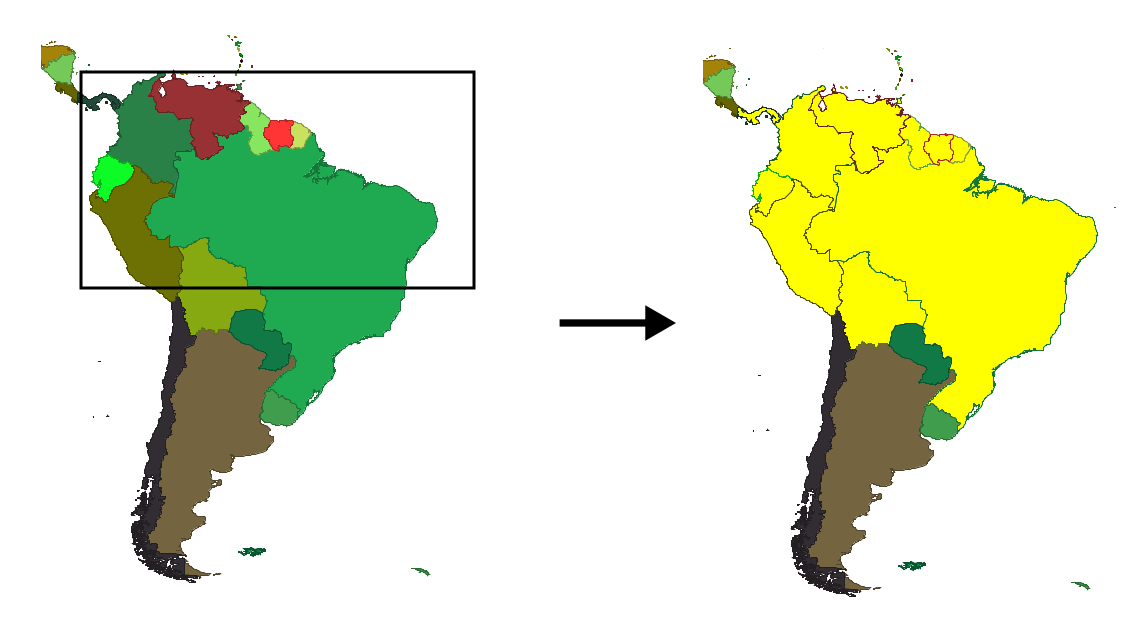
\includegraphics[width=\textwidth]{Bases_datos/Seleccion_rectangulo.png}
\caption{\small Una consulta sencilla mediante la definici�n gr�fica de un rect�ngulo. Todas las entidades dentro de este son el resultado de la consulta y quedan seleccionadas en el SIG.}
\label{Fig:Seleccion} 
\end{figure}


Una consulta nos vale tambi�n para extraer informaci�n de una base de datos de acuerdo a nuestras necesidades, y para crear posteriormente y a partir de dicha informaci�n una nueva capa. Esta operaci�n es �til cuando la base de datos de la que disponemos es muy voluminosa y solo resulta de inter�s para nuestro trabajo una parte de ella. Puede tratarse de una parte en el sentido espacial (la base de datos contiene datos a nivel mundial y se quiere trabajar a nivel estatal), en el sentido tem�tico (la base de datos contiene mucha informaci�n de cada entidad y solo interesan algunos campos), o en una combinaci�n de ambas. Para extraer dicha parte y trabajar �nicamente con ella, utilizaremos una consulta.

Veamos algunos ejemplos de consultas. Sea  una capa con los distintos pa�ses del mundo y una serie de valores econ�micos y sociales asociados a cada uno de ellos. Consideremos las siguientes preguntas:

\begin{itemize}
 \item �Qu� pa�ses tienen un Producto Interior Bruto mayor que el de Espa�a?
\item �Qu� pa�ses han experimentado un crecimiento econ�mico en el �ltimo a�o?
\item �Cu�ntos pa�ses tienen m�s de 200 millones de habitantes? 
\end{itemize}

En todos estos casos estamos haciendo referencia a pa�ses, los cuales, como sabemos, estar�n asociados a elementos geom�tricos que definan sus propiedades espaciales, es decir, a una componente espacial. Esta componente es la que permite que, adem�s de poder plantear las consultas anteriores, podamos representar cada pa�s en la pantalla y visualizarlo, o saber cu�les de ellos se encuentran en el hemisferio norte (esta ser�a una consulta espacial, de las que m�s adelante en este mismo cap�tulo veremos).

Sin embargo, cuando realizamos consultas como las tres anteriores, no acudimos para nada a la componente espacial. Consultas como estas podr�an resolverse si en lugar de una capa dentro de un SIG tuvi�ramos, por ejemplo, un simple anuario estad�stico lleno de tablas con datos correspondientes a cada pa�s. 

Las consultas pueden incluir varios criterios en una sola pregunta. Por ejemplo:

\begin{itemize}
 \item �Qu� pa�ses de la zona euro tienen m�s de 40 millones de habitantes?
\item �En qu� pa�ses de habla inglesa aument� la poblaci�n durante el �ltimo a�o?
\end{itemize}

Para expresar esas consultas se han de incluir elementos de la denominada \textbf{l�gica booleana}\footnote{Denominada as� por el matem�tico irland�s George Boole(1815, 1864)}. Esta implica el uso de \textbf{operadores l�gicos}, mediante los cuales se reescribir�an las consultas anteriores de la siguiente manera:

\begin{itemize}
 \item �Qu� pa�ses tienen como moneda el euro \emph{y} a la vez tienen m�s de 40 millones de habitantes?
\item �Que pa�ses hablan ingl�s \emph{y} sufrieron un aumento de poblaci�n durante el �ltimo a�o?
\end{itemize}

Los lenguajes de consulta que se emplean para transmitir estas operaciones a un SGBD, permiten el uso de tales operadores para formular consultas.

Si el SGBD es de tipo espacial y \emph{entiende} que algunas de las columnas de una tabla continene informacion espacial (es decir, que cada entidad no solo tiene informacion tem�tica), pueden plantearse consultas que hacen uso de esta, tales como las siguientes.

\begin{itemize}
\item �Qu� pa�ses comparten frontera con Alemania?
\item �Cu�ntos pa�ses se encuentran completamente en el hemisferio sur?
\item �Qu� pa�ses est�n a menos de 2000 km de Espa�a?
\end{itemize}

Para dar respuesta a esas cuestiones, basta analizar la componente espacial y no necesitamos para nada los datos con los que hemos trabajado anteriormente. Son consultas puramente espaciales. Aunque estas consultas ampl�an lo que ya conocemos, en realidad no abren ninguna nueva v�a de estudio de los datos geogr�ficos. Son consultas a las que podr�amos responder utilizando un mero mapa impreso, sin aprovechar el hecho de que dentro de un SIG las componentes espacial y tem�tica se hallan �ntimamente vinculadas. La verdadera potencia de las consultas espaciales la encontramos en la combinaci�n de estas consultas sobre la componente espacial y las que vimos anteriormente sobre la componente tem�tica. As�, se pueden plantear, por ejemplo, cuestiones como:

\begin{itemize}
 \item �Qu� pa�ses del hemisferio norte tiene una densidad de poblaci�n mayor que la de Per�?
\item �Cu�ntos pa�ses con m�s de 10 millones de habitantes se encuentran a menos de 1000 km de la frontera de Rusia?
\end{itemize}

Estas consultas incorporan elementos que hacen necesario acudir a la tabla de atributos, y otros que requieren analizar la componente espacial, estudiando las relaciones espaciales y topol�gicas de las geometr�as asociadas. 

Las consultas pueden incluir \textbf{varias capas}. Por ejemplo, si ademas de la capa de pa�ses disponemos de una capa de r�os del mundo, podr�amos responder a la pregunta \emph{�qu� pa�ses atraviesa el Nilo?}


Igualmente, las uniones entre tablas que hemos visto para el caso de la componente tem�tica pueden establecerse mediante un criterio espacial. Se tiene as� una \textbf{uni�n espacial}.

Un ejemplo muy sencillo de uni�n espacial es el que encontramos si combinamos la capa de pa�ses del mundo que venimos utilizando con una capa de ciudades del mundo. Podemos unir a la tabla de esta segunda capa todos los valores que caracterizan al pa�s al que pertenece cada ciudad. Si existe un campo com�n entre ambas tablas de atributos (por ejemplo, el nombre del pa�s), esto servir�a para efectuar esta uni�n. No obstante, esto no es necesario, ya que existe otro elemento com�n que no se encuentra almacenado dentro de la tabla, pero que puede tomarse de la componente espacial: toda ciudad debe estar situada dentro de los l�mites del pa�s al que pertenece. Esto sirve para establecer la relaci�n entre las tablas, y cada ciudad debe relacionarse con aquella entidad dentro de cuya geometr�a se encuentre el punto que la representa.



\subsection{�ndices espaciales}
\label{Indices_espaciales}


Si realizamos una consulta a una base de datos, el resultado es un subconjunto de esta con los elementos que cumplen el criterio expresado en la consulta. Si se implementa de forma \emph{directa} dicha consulta, esta operaci�n implica comprobar todos los elementos de la base de datos y ver cu�les son los que cumplen con el citado criterio. Teniendo en cuenta que una base de datos puede tener un gran tama�o, esta forma de proceder no es la �ptima.

Los �ndices nos permiten \emph{alcanzar} los elementos que constituyen la respuesta a nuestra consulta, haci�ndolo de la forma m�s r�pida y llegando hasta ellos sin tener que pasar por todos los restantes.

Un ejemplo f�cil de entender es el de una gu�a telef�nica en la que los nombre est�n ordenados alfab�ticamente. Gracias a ese orden y a que se conoce el alfabeto, se puede buscar rapidamente un nombre sin necesidad de leer todos ellos.

Al utilizar una base de datos, si no disponemos de un �ndice deberemos recorrer toda ella para dar respuesta a nuestras consultas. No sabemos \emph{d�nde} buscar las respuestas a nuestras consultas, del mismo modo que si en una guia telef�nica no supi�ramos que carece de sentido buscar en la letra F el n�mero telef�nico del se�or P�rez.

Ademas de �ndices para datos de tipo num�rico o texto, en los que resulta obvio establecer un orden natural, en el �mbito de los SIG tienen importancia los denominados \textbf{�ndices especiales}. Aunque sus fundamentos te�ricos son distintos, el concepto es similar al de �ndices de bases de datos no espaciales: elementos que permiten optimizar las consultas mediante una correcta estructuraci�n de los datos, en particular en este caso de su componente espacial.

Puede enterderse la idea de un �ndice espacial mediante un sencillo ejemplo de c�mo empleamos ideas parecidas a los �ndices espaciales de forma natural cuando tratamos de resolver una consulta espacial sin la ayuda de un SIG. Supongamos que tenemos nuestro mapa de pa�ses del mundo y queremos averiguar qu� pa�ses tienen su frontera a menos de 3000 kil�metros de la frontera de Espa�a. �C�mo operar�amos de manera natural para dar respuesta a esta consulta?

La soluci�n m�s inmediata es medir la distancia entre Espa�a y todos los pa�ses restantes, y despu�s tomar aquellos que hayan arrojado un resultado de distancia menor a 3000. La operaci�n dar�a el resultado esperado, pero implicar�a un gran n�mero de mediciones, y no ser�a una forma �ptima de operar. M�s probable es que no efectuemos mediciones con los pa�ses de Am�rica, pues un conocimiento b�sico de geograf�a basta para saber que todos ellos se encuentran a m�s de 3000 kil�metros. No sabemos exactamente a qu� distancia se encuentran, pero sabemos que no van a cumplir el criterio establecido en la consulta. 

Ese conocimiento b�sico de geograf�a que tenemos es en realidad una especie de �ndice espacial. No sirve para saber las distancias exactas ni resolver la consulta por completo, pero sirve para dar una aproximaci�n y facilitar el trabajo. Descartamos un buen numero de pa�ses de forma casi inmediata, y luego solo realizamos las operaciones costosas (la medici�n) con un subconjunto del total. 

De modo similar, los �ndices espaciales nos permiten obtener resultados en un �rea concreta sin necesidad de analizar todo el espacio ocupado por el total de los datos. Gracias a ello, hacen las consultas mas efectivas y permiten trabajar con grandes vol�menes de datos.

Los �ndices espaciales se almacenan junto con los datos a los que hacen referencia, bien en ficheros adicionales o dentro de la propia base de datos, en case de utilizarse una. Los SGBD espaciales tienen capacidades para calcular estos �ndices espaciales y almacenarlos en la base de datos, recurriendo a ellos cuando se realiza una consulta que requiera su uso.


\pagestyle{empty}

\chapter{An�lisis espacial. Fundamentos}
\label{Introduccion_procesos}


\pagestyle{fancy}

El an�lisis espacial es una de las tareas fundamentales sin las cuales el concepto de SIG no alcanza su verdadero significado. 

El an�lisis espacial es el \textbf{estudio cuantitativo de aquellos fen�menos que se manifiestan en el espacio}. Ello indica una importancia clave de la posici�n, la superficie, la distancia y la interacci�n a trav�s del propio espacio. 

Ejemplos de an�lisis que realizamos con cartograf�a fuera de un SIG son el buscar en un mapa d�nde se sit�a el pico m�s alto, ver la elevaci�n concreta a la que se encuentra un elemento dado tal como una poblaci�n, o planificar una jornada tur�stica viendo qu� lugares de inter�s podemos visitar o c�mo llegar desde uno a otro de estos lugares haci�ndolo por las mejores carreteras o de la forma m�s r�pida. Estas actividades habituales son ejemplos de an�lisis geogr�ficos que podemos igualmente realizar dentro de un SIG.

Mediante el an�lisis podemos generar nuevos datos que pueden ser \textbf{nuevas capas de datos geogr�ficos, tablas de datos, valores escalares} o \textbf{vectores}.

En ocasiones, los resultados expresan \textbf{la misma variable} que el dato de partida (por ejemplo, el c�lculo de una media), y en otros las variables de entrada y salida son \textbf{distintas} (por ejemplo, si a partir de una capa de elevaciones calculamos una de pendientes).

Asimismo, todo an�lisis espacial parte de un conjunto de datos espaciales, pudiendo estos ser \textbf{de un �nico tipo, o de varios distintos} que se combinan en un procedimiento concreto. Por ejemplo, en el caso de calcular la localizaci�n del punto m�s alto, el resultado es una sencilla coordenada, y tan solo se utiliza la variable elevaci�n. En el caso de la altura media de una ciudad, se utilizan dos entradas: por un lado, la elevaci�n, y por otro, el emplazamiento de la ciudad. Aunque un mapa cl�sico contiene toda esa informaci�n en una �nica hoja, en realidad son dos elementos distintos combinados a la hora de representarlos. En t�rminos m�s acordes con un SIG, podemos decir que tenemos dos capas distintas que utilizamos como entradas.

El an�lisis dentro un SIG nos permite tanto formular como responder a cuestiones. Estas cuestiones pueden ser:

\begin{itemize}
 \item Relativas a posici�n y extensi�n
\item Relativas a la forma y distribuci�n
\item Relativas a la asociaci�n espacial
\item Relativas a la interacci�n espacial
\item Relativas a la variaci�n espacial
\end{itemize}

Algunos ejemplos de an�lisis geogr�fico son los siguientes.

\begin{itemize}
\item \textbf{Consulta espacial}. Vimos las consultas en detalle dentro del cap�tulo dedicado a las bases de datos.

\item \textbf{An�lisis topol�gico}. Pueden plantearse consultas referidas no solo a la posici�n de los elementos geogr�ficos, sino a la \textbf{relaci�n con otros elementos}. La existencia de topolog�a puede emplearse para la realizaci�n de consultas que respondan a cuestiones como:

\subitem �C�mo llegar desde mi posici�n actual hasta una coordenada concreta por la red viaria existente?

\subitem �Qu� comunidades aut�nomas comparten l�mite con Madrid?

\item \textbf{Medici�n}. La existencia de una referencia espacial para cada uno de los elementos con los que trabajamos en el an�lisis dentro de un SIG hace que podamos \textbf{cuantificar} otra serie de par�metros tambi�n espaciales. Entre las mediciones m�s b�sicas, encontramos las distancias, �reas, per�metros o factores de forma. Mas elaboradas, encontramos otras como pendientes o indices derivados de medidas simples.


\item \textbf{Combinaci�n}. Uno de los procedimientos m�s habituales y m�s caracter�sticos dentro del uso de un SIG es la \textbf{combinaci�n o superposici�n} de varias capas de informaci�n. La propia estructura de la informaci�n geogr�fica en capas facilita notablemente estos procedimientos y convierte a los SIG en plataformas ideales para llevar a cabo an�lisis donde se combina informaci�n sobre diversas variables.



\item \textbf{Transformaciones}. Podemos englobar dentro de este grupo una amplia serie de procedimientos que modifican los elementos de entrada de diversas formas. Entre los m�s habituales, encontramos la \textbf{transformaci�n de coordenadas}, la \textbf{simplificaci�n de geometr�as}, o la \textbf{creaci�n de �reas de influencia} o la \textbf{reclasificaci�n de valores}. Estas transformaci�n pueden afectar tanto a la componente espacial como a la componente tem�tica del dato. 

\item \textbf{An�lisis de superficies}. El an�lisis de superficies es uno de los m�s potentes de cuantos encontramos en un SIG. Desde par�metros b�sicos como la \textbf{pendiente} o la \textbf{orientaci�n} hasta par�metros morfom�tricos muy espec�ficos, pasando por todas las herramientas del \textbf{an�lisis hidrol�gico}, la bater�a de operaciones disponibles es muy amplia. 

\item \textbf{Estad�stica descriptiva}. Los elementos de la estad�stica cl�sica tienen sus equivalentes en los datos espaciales, y nos permiten \textbf{calificar cuantitativamente} los datos con los que trabajamos. Se incluyen aqu� descriptores de centralidad y dispersi�n, de dependencia espacial o el estudio de patrones espaciales, entre otros muchos. Estos pueden a su vez usarse para el contraste de hip�tesis que contengan una cierta componente espacial.

Por ejemplo, estos estad�sticos nos permiten dar respuesta a cuestiones del tipo

\subitem �Es constante la media de altura a lo largo de toda la geograf�a de mi pa�s?

\subitem �Existe alguna direcci�n predominante en los movimientos de individuos de una especie o se desplazan err�ticamente?

\item \textbf{Inferencia}. Otro an�lisis estad�stico de gran importancia en los SIG es el que permite inferir comportamientos de las distintas variables y estudiar, por ejemplo, la forma en que estas van a evolucionar a lo largo del tiempo.

El establecimiento de modelos de cambio y variaci�n representa una de las herramientas m�s actuales en el campo de los SIG, y un campo en abundante desarrollo.

\item \textbf{Toma de decisiones y optimizaci�n}. La estructura de la informaci�n geogr�fica en capas dentro de un SIG, favorable como ya vimos para la superposici�n de capas, lo es igualmente para estudiar de forma combinada los efectos de distintos factores. Este estudio nos permite luego responder a cuestiones como, por ejemplo,

\subitem �Cu�l es el mejor lugar para emplazar una nueva construcci�n en funci�n de su impacto sobre el medio?

\subitem �D�nde situar un nuevo hospital para que el servicio en la comarca mejore lo m�ximo posible?

\item \textbf{Modelizaci�n}. La creaci�n de modelos espaciales dentro de un SIG es una tarea a�n pendiente de mucho desarrollo. No obstante, existe un gran n�mero de modelos en los m�s diversos campos, y la arquitectura de datos y procesos de los SIG es propicia para la implementaci�n de otros nuevos.
\end{itemize}

\section{Particularidades de los datos espaciales para su an�lisis}
\label{Analisis_espacial}


Las caracter�sticas propias de los datos espaciales dotan a estos de una \textbf{gran potencialidad} de an�lisis, al tiempo que \textbf{condicionan o limitan} otras operaciones. Algunas de estas caracter�sticas representan problemas que han de tenerse presentes en el an�lisis; otros son simplemente conceptos b�sicos que deben conocerse pero no han de implicar necesariamente una dificultad asociada.

\subsection{Escala}
\label{Escala_analisis}

A la hora de estudiar la informaci�n geogr�fica, podemos hacerlo a \textbf{distintos niveles} y, dependiendo del nivel elegido, los resultados ser�n de una u otra naturaleza. Debido a esto, adem�s de considerar la escala cartogr�fica para la representaci�n y gesti�n de datos en un SIG, es necesario considerar la \textbf{escala de an�lisis}.

La escala de an�lisis depende \textbf{del dato en s�} (precisi�n, tipo, etc.), as� como del \textbf{an�lisis que se va a realizar} con �l.

Como se muestra en la figura \ref{Fig:Escalas_formas_terreno}, si para definir las formas de relieve en un punto dado lo hacemos considerando dicho punto y los valores de elevaci�n a su alrededor, la caracterizaci�n que hagamos var�a en funci�n de la dimensi�n de esa zona alrededor (que es la que define la escala de an�lisis). Para valores peque�os de dicha zona de an�lisis, el punto analizado puede definirse como una cima, mientras que aumentando la escala de an�lisis se advierte que el punto se sit�a en el fondo de un valle.

\begin{figure}[h]   
\centering
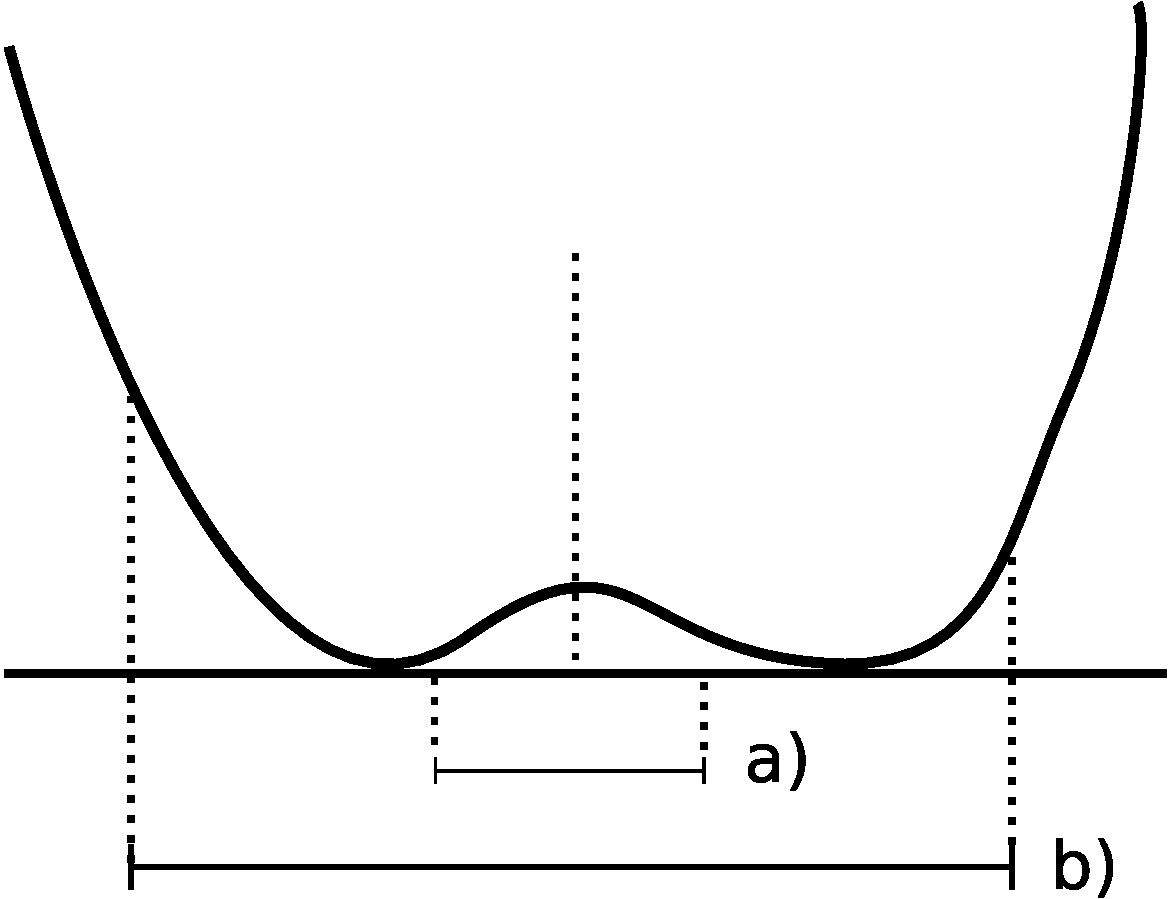
\includegraphics[width= .45\mycolumnwidth]{Analisis_espacial/Escalas_formas_terreno.pdf}
\caption{\small Dependiendo de la escala de an�lisis, un mismo relieve puede ser caracterizado como cima (a) o fondo de valle (b)}
\label{Fig:Escalas_formas_terreno} 
\end{figure}

Por tanto, debemos observar el relieve desde la distancia correcta a la cual la informaci�n que nos proporciona es la m�s adecuada para un an�lisis dado. Adem�s de existir una escala de mayor relevancia para un an�lisis concreto,  es de inter�s el trabajar a \textbf{m�ltiples escalas} y combinar los resultados.

Otro ejemplo de c�mo la escala de an�lisis condiciona los resultados obtenidos lo encontramos en el caso de efectuar \textbf{mediciones}. Como puede verse en la figura \ref{Fig:Medida_linea_fractal}, la unidad de medida empleada provoca que se obtengan resultados distintos. 

\begin{figure}[h]   
\centering
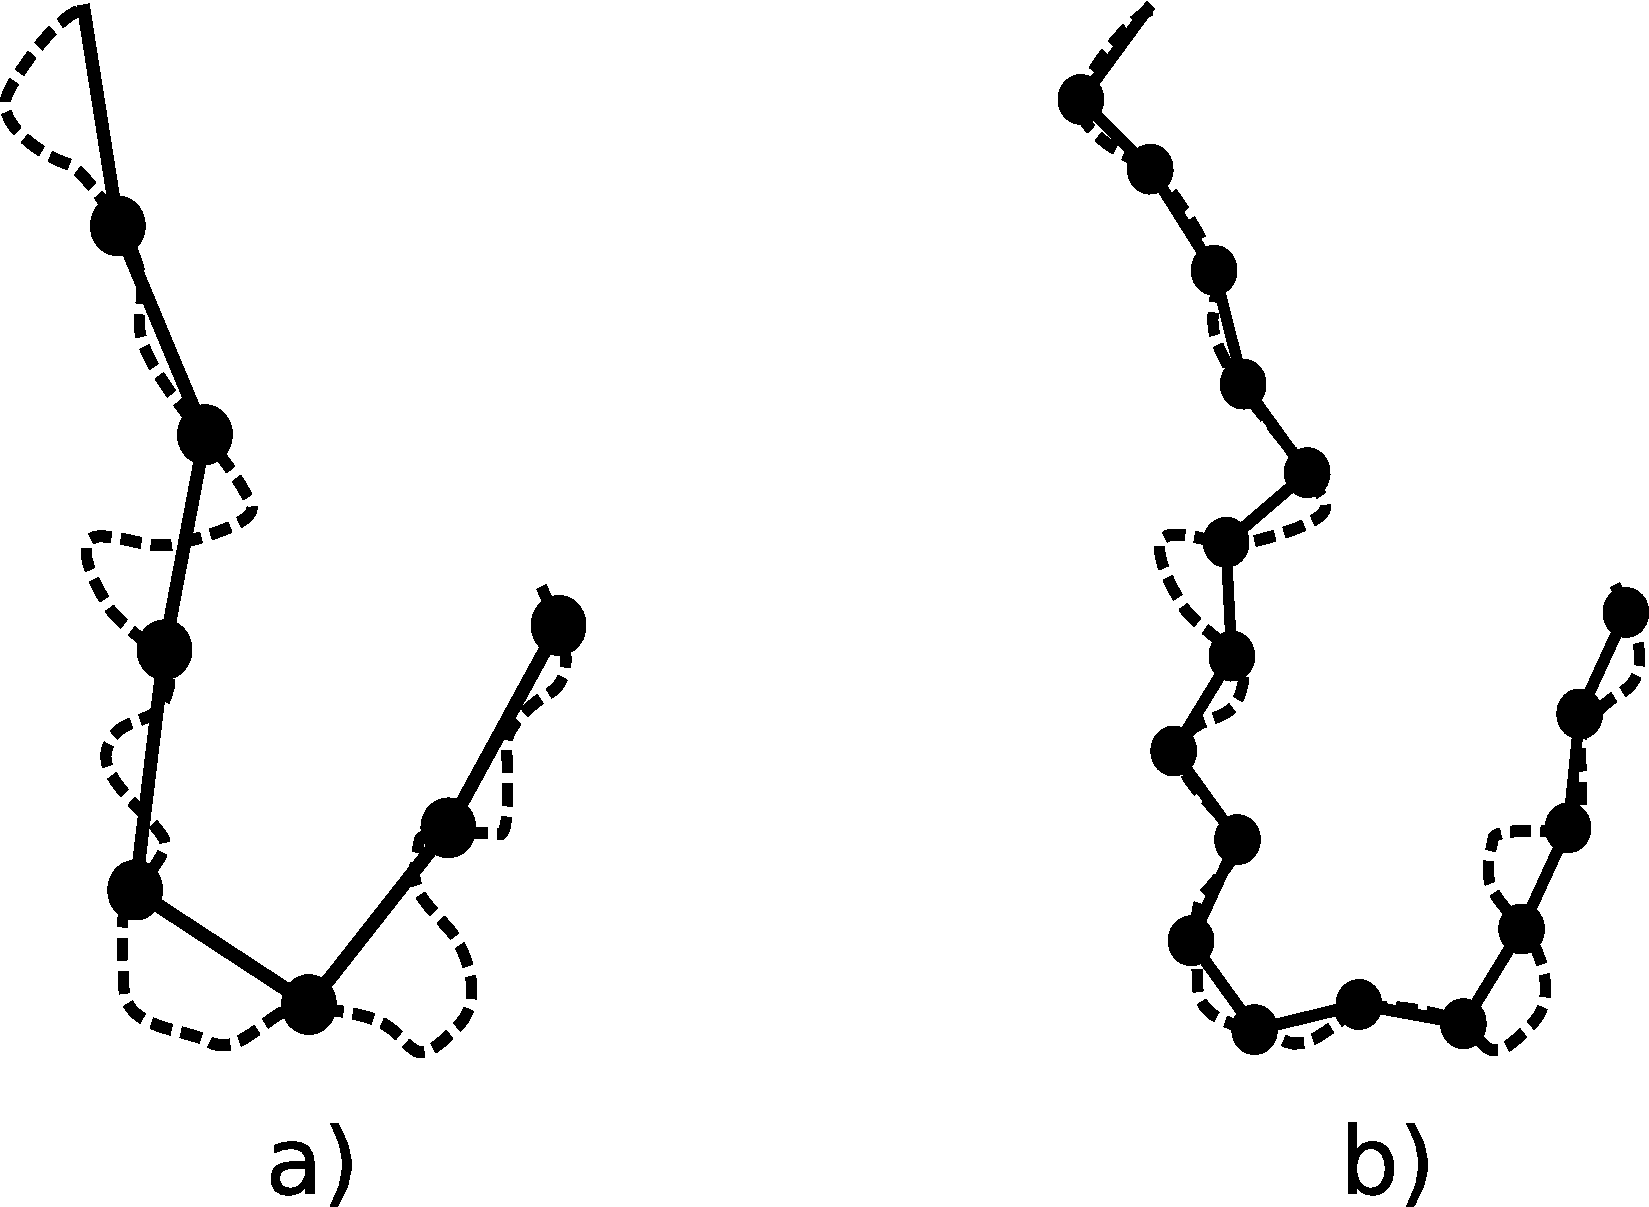
\includegraphics[width= .45\mycolumnwidth]{Analisis_espacial/Medida_linea_fractal.pdf}
\caption{\small La unidad de medida empleada modifica el resultado obtenido.}
\label{Fig:Medida_linea_fractal} 
\end{figure}

La uni�n del valor resultante con la escala a la que se ha obtenido tiene en conjunto pleno significado, pero ese valor por s� mismo carece de dicho significado. 

El concepto de \textbf{fractal} tiene una implicaci�n directa en este hecho.

El propio \textbf{formato de almacenamiento} condiciona el efecto de la escala, ya que puede imponer l�mites. Tal es el caso cuando se trabaja con capas raster, en las que el \textbf{tama�o de celda} delimita la precisi�n que puede obtenerse en el an�lisis.

\subsection{El Problema de la Unidad de �rea Modificable}
\label{MAUP}

Muchas de las variables con las que trabajamos dentro de un SIG \textbf{no pueden medirse de forma puntual}, y por ello han de \textbf{estudiarse para un �rea dada}. Ejemplos de este tipo de variables son el porcentaje de poblaci�n en un rango de edad determinado o la densidad media de poblaci�n.

Las �reas que se definen para poder trabajar con las variables de esta �ndole son \textbf{esencialmente arbitrarias}, tales como pa�ses, regiones o distritos, que se establece sin ning�n criterio propio del an�lisis espacial. La utilizaci�n de una u otra unidad \textbf{altera los resultados} extra�dos de las variables estudiadas.

Este problema, por tener relaci�n con la elecci�n de la unidad de agregaci�n de la informaci�n, se conoce como \emph{Problema de la Unidad de �rea Modificable}(PUAM).


Un problema particular relacionado con el PUAM es la denominada \textbf{falacia ecol�gica}, que consiste en asumir que los valores calculados para una unidad de �rea pueden aplicarse a los individuos de la poblaci�n existente en dicha �rea. S�lo en el caso de que exista una completa homogeneidad para la variable analizada, lo cual raramente sucede, la anterior suposici�n ser�a cierta.

\subsection{Autocorrelaci�n espacial} 
\label{Autocorrelacion_espacial}

Se denomina \textbf{autocorrelaci�n espacial} a la existencia de una \textbf{correlaci�n de la variable consigo misma}, de tal modo que los valores de esta variable en un punto guardan relaci�n directa con los de esa misma variable en otros puntos cercanos. Por ejemplo, en el caso de medirse la temperatura, los puntos cerca de un foco de calor tendr�n una temperatura mayor que aquellos cerca de focos fr�os. Si estudiamos la distribuci�n de una enfermedad infecciosa, es m�s probable que los casos se encuentren agrupados, de forma que la presencia de un alto n�mero de casos implique tambi�n una alta incidencia en poblaciones cercanas.

Otra forma de expresar la autocorrelaci�n espacial es mediante la conocida como \textbf{Primera Ley Geogr�fica de Tobler}, que establece que <<todo est� relacionado con todo, pero las cosas pr�ximas entre s� est�n m�s relacionadas que las distantes>>.

La autocorrelaci�n espacial, tal y como se ha descrito antes, es \textbf{positiva}. Puede, no obstante, existir una \emph{autocorrelaci�n espacial negativa}, si los valores altos se rodean de valores bajos y viceversa.

En caso de no existir ning�n tipo de autocorrelaci�n espacial, se tiene que los datos recogidos en una serie de puntos son \textbf{independientes entre s�} y no se afectan mutuamente, sin que tenga influencia de la distancia.

La figura \ref{Fig:Autocorrelacion_espacial} muestra unas sencillas capas r�ster en las que se presentan los tres tipos de autocorrelaci�n espacial anteriores.

\begin{figure}[!hbt]   
\centering
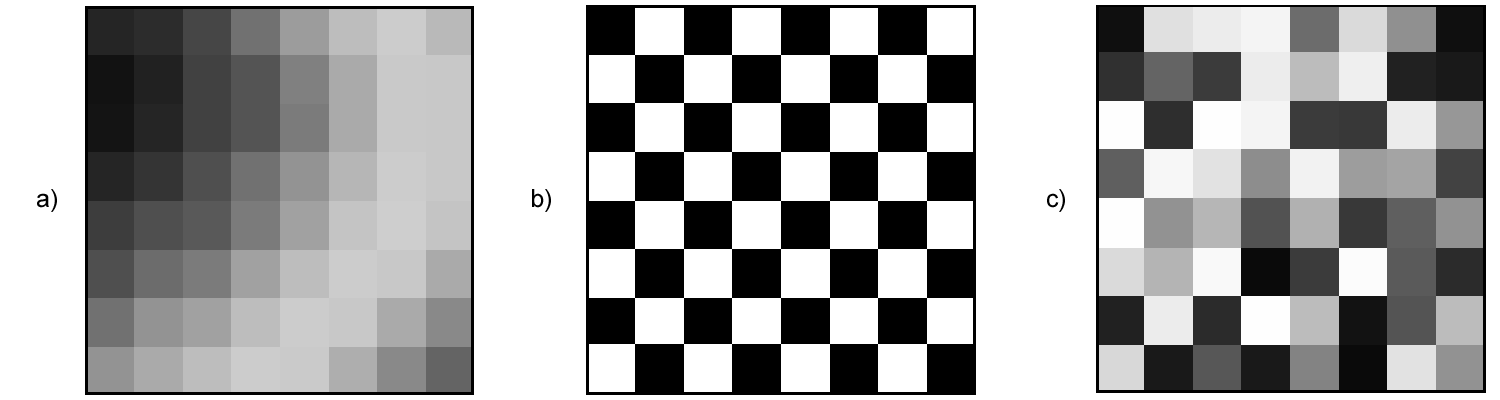
\includegraphics[width=\textwidth]{Analisis_espacial/Autocorrelacion_espacial.png}
\caption{\small a) Autocorrelaci�n espacial positiva. b) Autocorrelaci�n espacial negativa. c) Ausencia de autocorrelaci�n espacial (independencia)}
\label{Fig:Autocorrelacion_espacial} 
\end{figure}

Las consecuencias de la existencia de autocorrelaci�n espacial son numerosas y de gran importancia.

Por una parte, muchos de los an�lisis estad�sticos suponen la \textbf{independencia de la variable}. Puesto que existe una dependencia de la componente espacial, ser� necesario para obtener resultados correctos introducir dicha componente espacial como una variable m�s. 

Algo similar sucede cuando los datos presentan alguna \textbf{tendencia espacial} (los valores de una variable est�n relacionados con sus propias coordenadas geogr�ficas), ya que esto tambien invalida el supuesto de la independencia de los datos.

Existiendo autocorrelaci�n espacial, y siendo esta positiva, la \textbf{inferencia estad�stica es menos eficaz} que si se cuenta con un n�mero igual de observaciones de una variable independiente. 

La autocorrelaci�n espacial no es, no obstante, un elemento que siempre tenga consecuencias negativas. Puesto que los puntos cercanos a uno dado guardan relaci�n con este, la autocorrelaci�n puede aprovecharse para \textbf{estimar valores} en un punto cualquiera si conocemos los valores en puntos cercanos. Este es el fundamento de los \textbf{m�todos de interpolaci�n}


\subsection{Existencia de estructura}

Tanto la disposici�n de los datos como las propiedades de la variable estudiada (por ejemplo, la propia autocorrelaci�n espacial como propiedad intr�nseca) exhiben una estructura determinada. Esta estructura puede condicionar los resultados del an�lisis y tener influencia sobre estos.

Los dos principales conceptos estad�sticos que definen la estructura espacial de los datos son la \textbf{estacionaridad} y la \textbf{isotrop�a}. La estacionaridad indica que el proceso es \textbf{invariante a la traslaci�n}. Es decir, que las propiedades son constantes en el espacio y no existe tendencia alguna. La isotrop�a indica que el proceso es \textbf{invariante a la rotaci�n} y tiene lugar del mismo modo en todas direcciones. 


\subsection{Efectos de borde}
\label{EfectoBorde}

Las zonas que estudiamos dentro de todo an�lisis espacial \textbf{tienen unos l�mites establecidos}. Estos l�mites vienen definidos de forma artificial ---el l�mite de la fotograf�a a�rea de la que disponemos, por ejemplo--- o bien de forma natural ---si estudiamos un bosque junto a un pantano, el bosque encuentra su l�mite al borde de este �ltimo---. La presencia de estos bordes \textbf{distorsiona el resultado de los an�lisis}, en especial para aquellos par�metros no puntuales que requieren la definici�n de un area de estudio (densidades, etc., como ya vimos para el caso del PUAM)

La figura \ref{Fig:Efecto_borde} muestra un ejemplo de efecto de borde.

\begin{figure}[h]   
\centering
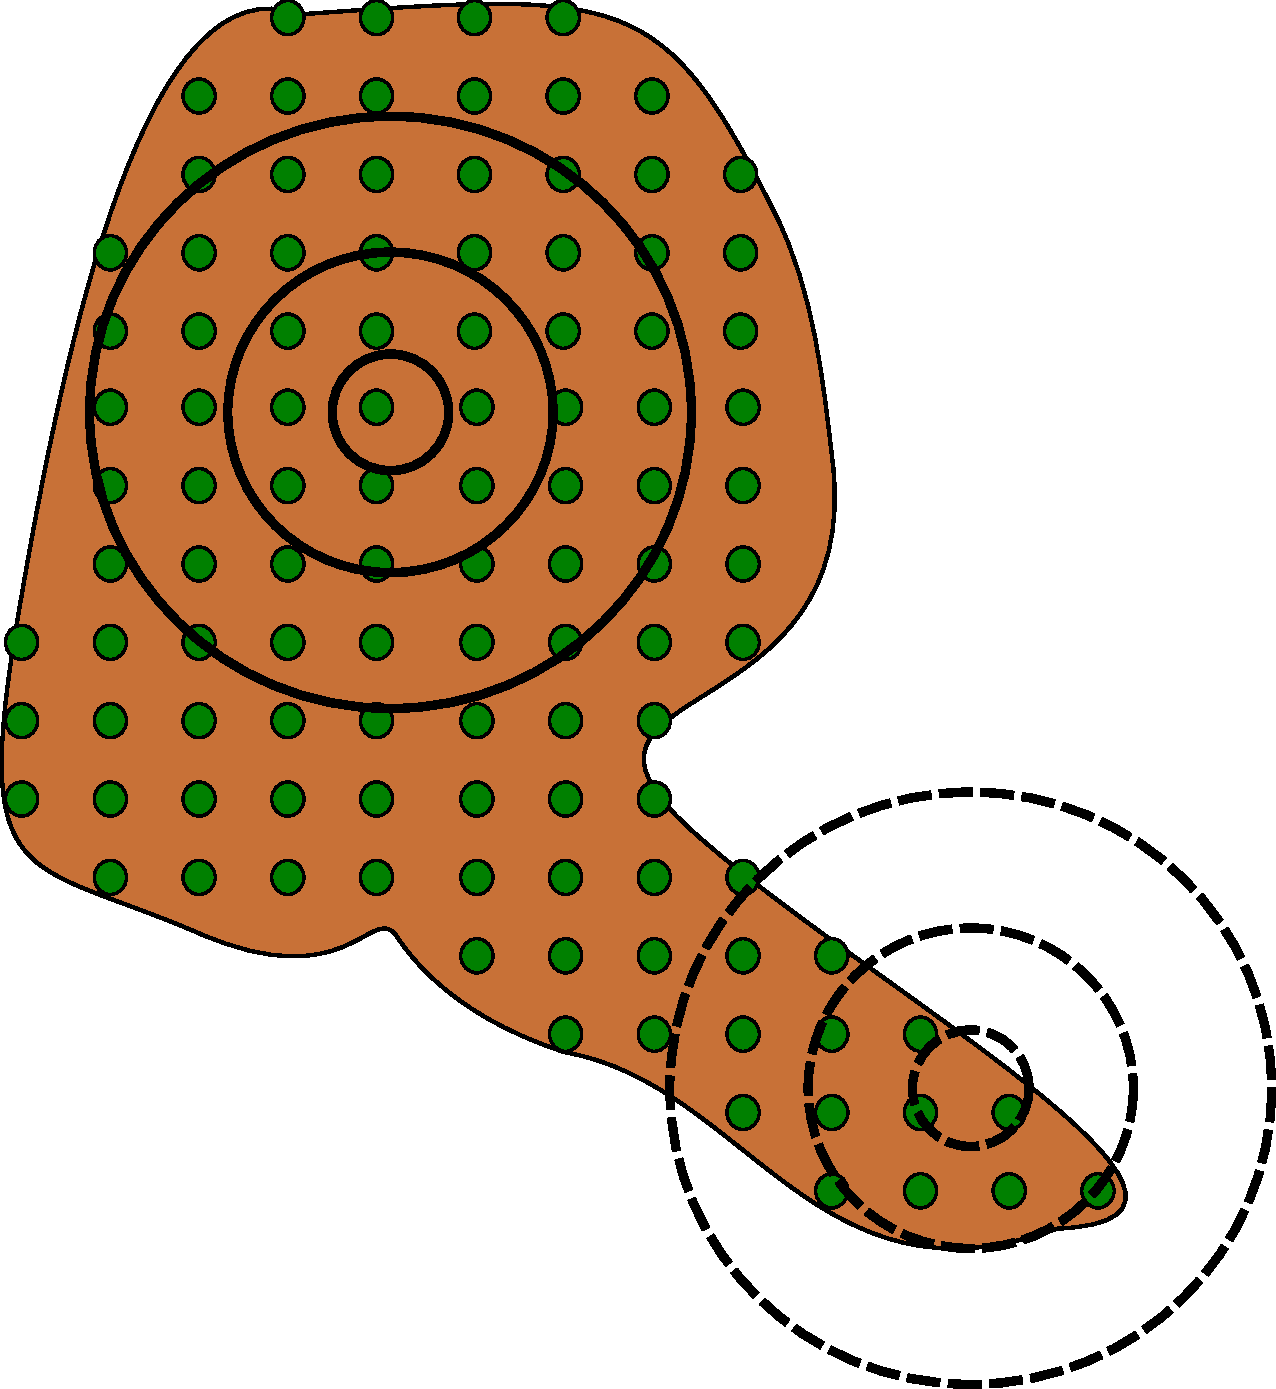
\includegraphics[width=.35\columnwidth]{Analisis_espacial/Efecto_borde.pdf}
\caption{\small Representaci�n del efecto borde y c�mo este afecta en mayor o menor medida en funci�n de la escala de an�lisis. Las zonas en trazo continuo no se ven afectadas. Las zonas en trazo punteado est�n afectadas de efecto de borde en diferente grado.}
\label{Fig:Efecto_borde} 
\end{figure}

En algunos casos, el efecto de borde no se manifiesta �nicamente para puntos cercanos a dicho borde, sino para \textbf{todos aquellos relacionados o conectados} con �l seg�n un determinado criterio, con independencia de su distancia a este.


\pagestyle{empty}
\chapter{Visualizaci�n y representaci�n de datos espaciales}
\label{Introduccion_visualizacion}


\pagestyle{fancy}

Visualizar la informaci�n geogr�fica es una parte fundamental del trabajo con un SIG. Aunque algunos datos incluyen su propia manera de representarse ---por  ejemplo, las im�genes de sat�lite, las ortofotos, o las obtenidas de un servicio de mapas---, en el SIG es en general el usuario quien define la forma de representar el dato. Es decir, el usuario de SIG toma el papel del cart�grafo, y por tanto debe conocer los fundamentos que este utiliza para la creaci�n de mapas.

Adem�s de las herramientas y conceptos cartogr�ficos cl�sicos, los SIG incorporan elementos de la denominada \textbf{visualizaci�n cient�fica}, tales como la interactividad o la representacion de datos multidimensionales. El resultado de este nuevo planteamiento, m�s rico que el de la cartograf�a cl�sica, se conoce como \textbf{geovisualizaci�n}. La diferencia entre la geovisualizacion y la cartograf�a cl�sica puede visualizarse mediante el  denominado \emph{Cubo cartogr�fico} (Figura \ref{Fig:CuboCartografico}).

\begin{figure}
\centering
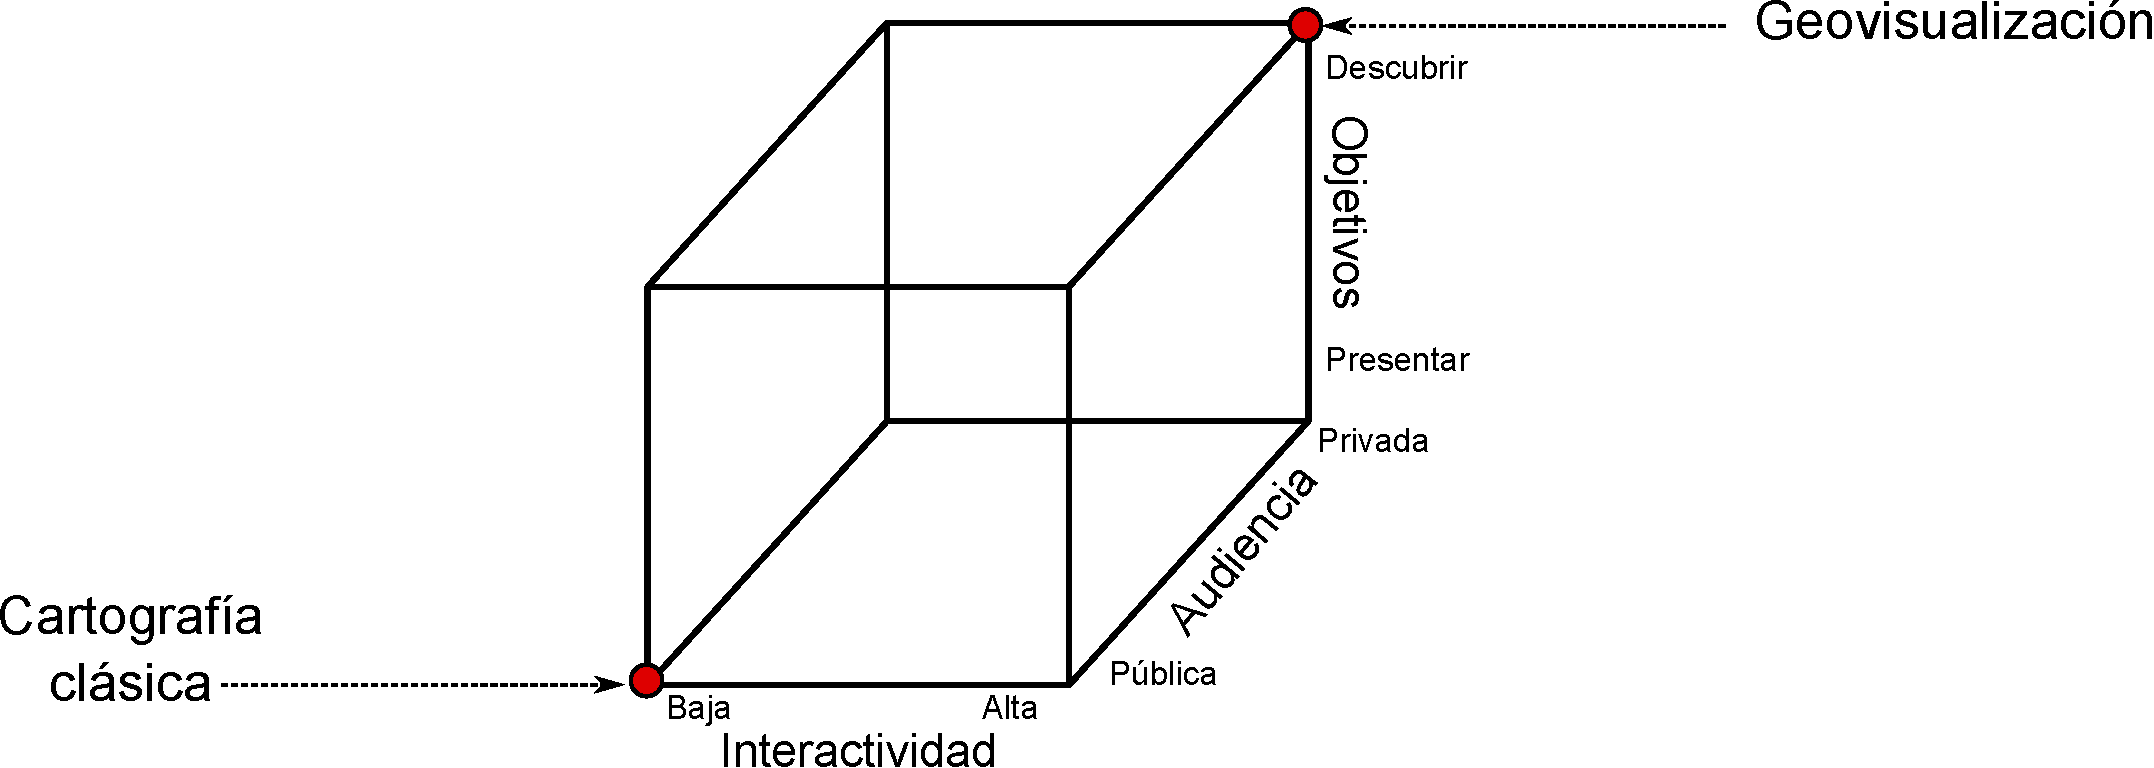
\includegraphics[width=\columnwidth]{Visualizacion/CuboCartografico.pdf}
\caption{\small El \emph{cubo cartogr�fico}.}
\label{Fig:CuboCartografico} 
\end{figure}

El cubo cartogr�fico contiene tres ejes, en los cuales se representan el grado de interactividad, el objetivo principal de la representaci�n y la audiencia a la que esta se dirige. La cartograf�a cl�sica y la geovisualizaci�n se sit�an en v�rtices opuestos, ya que presentan caracter�sticas distintas en estos tres conceptos. El mapa cl�sico esta pensado para presentar una informaci�n de la que ya se dispone, pero no es una herramienta para descubrir nueva informaci�n. La geovisualizaci�n, por el contrario, con la posibilidad que ofrece al usuario de <<explorar>> los datos, puede servir para extraer informaci�n que no se conoc�a de antemano a la hora de crear la representaci�n. La interactividad es alta en la geovisualizaci�n y baja en el mapa cl�sico, como ya hemos visto. Por �ltimo, la audiencia en la geovisualizaci�n es privada, entendi�ndose con esto no que existan restricciones para su acceso, sino que en su mayor�a son representaciones fugaces que cambian seg�n el usuario interact�a con el \emph{software}, y por tanto lo normal es que solo sea ese usuario quien las disfrute, no teniendo un car�cter persistente como el mapa impreso.

En este cap�tulo veremos las ideas fundamentales sobre la representaci�n de datos, tanto las empleadas en la cartograf�a tradicional como aquellas propias del �mbito de la geovisuliaci�n.




\section{Conceptos b�sicos de visualizaci�n}
\label{Conceptos_basicos_visualizacion}


Cuando visualizamos cualquier tipo de informaci�n geogr�fica, ya sea a trav�s de un mapa cl�sico o de alg�n elemento gr�fico en la pantalla de un ordenador, estamos utilizando un \textbf{lenguaje visual} para transmitirla. Del mismo modo que al hablar empleamos un lenguaje oral y al escribir un lenguaje escrito, siempre que plasmemos la informaci�n geogr�fica en una serie de elementos visuales estaremos empleando este lenguaje visual.


El estudio de los signos de un lenguaje constituye lo que se conoce como \textbf{semiolog�a}. En el caso de los elementos del lenguaje visual, encontramos una \textbf{semiolog�a gr�fica}. Esta semiolog�a trata los signos del lenguaje visual y la gram�tica de estos, definiendo una ling��stica visual que nos ayuda a comprender c�mo una representaci�n gr�fica dada cumple su prop�sito de transmitir la informaci�n en base a la cual se crea.


\subsection{Las variables visuales}

Existen diversas propiedades de los elementos visuales que podemos emplear para trasnmitir una informaci�n, siendo m�s adecuadas unas u otras seg�n sea la circunstancia.

\begin{figure}[!hbt]
\centering
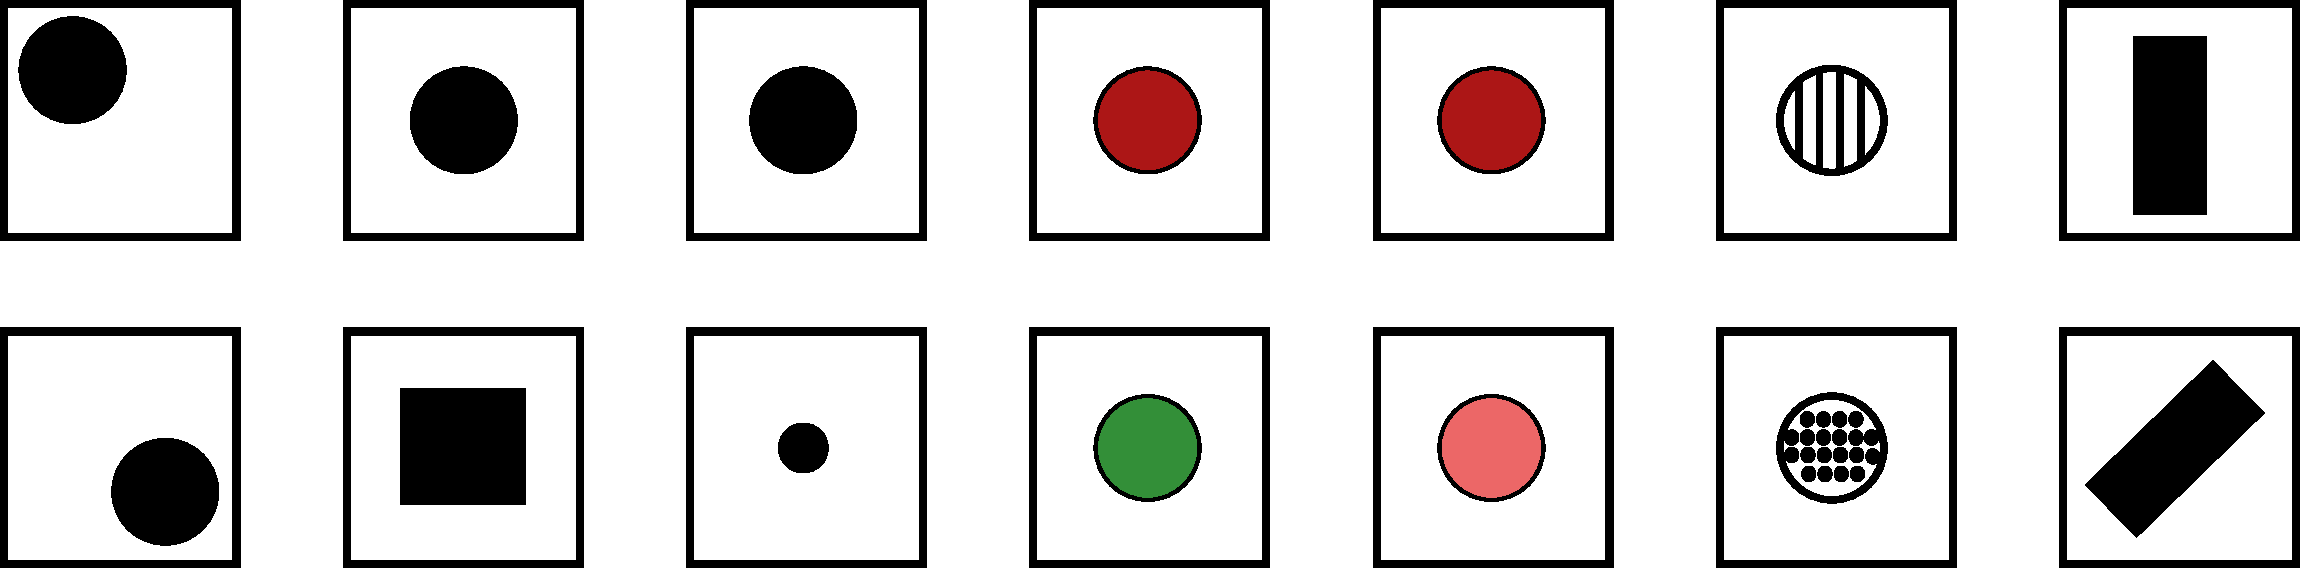
\includegraphics[width=\columnwidth]{Visualizacion/VariablesVisuales.pdf}
\caption{\small Ejemplo de uso de las distintas variables visuales. De izquierda a derecha: posici�n, forma, tama�o, tono, valor, textura, y orientaci�n}
\label{Fig:VariablesVisuales} 
\end{figure}


Estas propiedades conforman lo que se conoce como \emph{variables visuales}, y se aplican a los elementos b�sicos de la representaci�n, que son aquellos objetos geom�tricos de que se compone esta. Las variables visuales permiten diferenciar unos de otros y asignarles unas ciertas caracter�sticas, susceptibles a su vez de ser interpretadas junto al propio significado que el objeto pueda tener. Dados dos elementos, estos pueden diferenciarse por las siguientes variables, que aparecen representadas en la figura \ref{Fig:VariablesVisuales}: Posici�n, forma, tama�o, textura, color y orientaci�n

El uso de la \textbf{posici�n} est� muy restringido en el caso de un mapa, por deber respetarse el emplazamiento real en el espacio del elemento representado, y por ello y no se emplea.

La \textbf{forma} viene definida por el per�metro exterior del objeto. La forma se aplica fundamentalmente a los s�mbolos puntuales, situando un s�mbolo de una forma dada sobre las coordenadas exactas del punto a representar. Su aplicaci�n a s�mbolos lineales es dif�cil y no se da, mientras que en el caso de aplicarse sobre s�mbolos de superficie requiere la alteraci�n de los pol�gonos representados (por ejemplo, que tracen los l�mites de pa�ses), dando lugar a una representaci�n imprecisa, al menos en lo que al contorno del pol�gono respecta. 

El \textbf{tama�o} se refiere a la dimensi�n del s�mbolo. Para el caso de s�mbolos puntuales, puede aplicarse sin m�s que hacer m�s grande o peque�o el s�mbolo en s�. En el caso de l�neas, el grosor de estas constituye la forma de aplicar la variable tama�o. No se usa en s�mbolos superficiales, salvo aplic�ndolo sobre la textura de relleno.(Figura \ref{Fig:TamanoTexturas}).


\begin{figure}[!hbt]
\centering
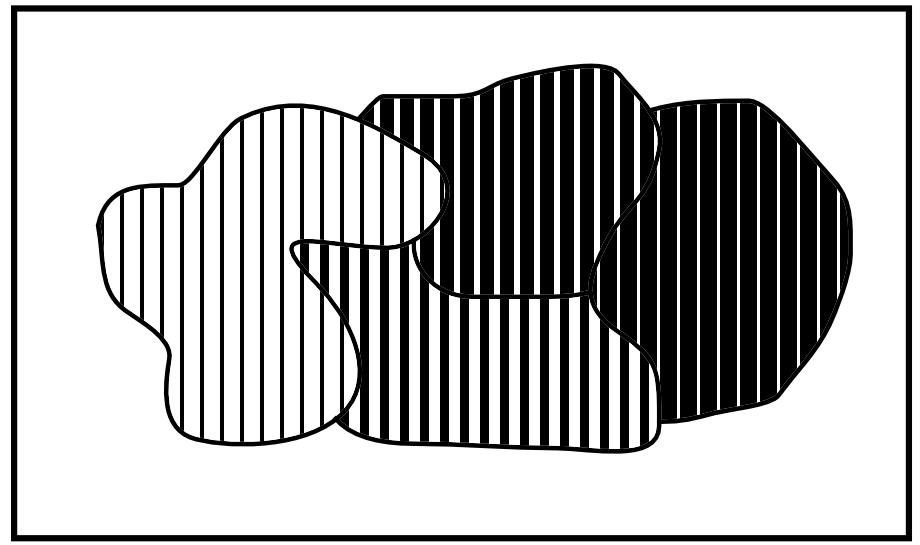
\includegraphics[width=.4\mycolumnwidth]{Visualizacion/Texturas.png}
\caption{\small Uso del tama�o en s�mbolos de superficie mediante texturas.}
\label{Fig:TamanoTexturas} 
\end{figure}


El tama�o condiciona la percepci�n de otras variables visuales, especialmente cuando se trata de tama�os peque�os. 

La \textbf{textura} hace referencia al relleno de un s�mbolo mediante alg�n patr�n. Se aplica en lineas mediante el uso de guiones y espacios en blanco que dan lugar a un patr�n de discontinuidad, aunque su uso principal es en el caso de s�mbolos de superficie.

El color es la m�s importante de todas las variables visuales, debido a las posibilidades que ofrece\footnote{Si estas leyendo una copia impresa de este libro, en blanco y negro, te recomiendo acudir a la versi�n digital, donde encontraras las im�genes en colores.}.

Dos son las componentes de un color que se utilizan como variables visuales, y que pueden entenderse como tales por si mismas: el tono y el  valor. 

El \textbf{tono} es lo que en el lenguaje com�n denominar�amos color, es decir el nombre del color, por ejemplo verde, rojo o amarillo. 

El tono puede verse alterado por los tonos del entorno, especialmente en s�mbolos de peque�o tama�o. Aunque es una variable para la que la percepci�n humana tiene gran sensibilidad, en los s�mbolos peque�os puede ser dif�cil de identificar y pueden producirse una falsa percepci�n si comparten espacio con otras m�s grandes de un tono distinto. 

Por su parte, el \textbf{valor} indica la claridad del color. Un tono azul puede ser m�s claro o m�s oscuro sin dejar de ser azul. Esa variaci�n que se produce es una variaci�n del valor del color. 

La capacidad de diferenciar dos s�mbolos con valor distinto var�a en funci�n del tipo de s�mbolo. As�, es mayor en el caso de s�mbolos de superficie, mientras que en el caso de s�mbolos puntuales y lineales est� relacionada con el tama�o. Si el punto es muy peque�o o la l�nea muy delgada, es m�s dif�cil apreciar el valor y, por tanto, comparar este con otro o extraer la informaci�n que mediante esa variable visual se intenta transmitir.


Por �ltimo, la \textbf{orientaci�n} se aplica sobre los s�mbolos puntuales, siempre que estos no presenten simetr�as que impidan percibir correctamente la orientaci�n. Para los s�mbolos de superficie, se aplica a trav�s de la textura, variando la orientaci�n de esta. No se aplica en el caso de l�neas.




\subection{Las propiedades de las variables visuales}

Las variables que acabamos de ver son ahora nuestras herramientas que emplearemos para simbolizar la informaci�n geogr�fica y sabemos ya c�mo aplicarlas. Lo que no hemos visto a�n es qu� capacidades tienen y qu� podemos simbolizar mediante ellas, y este es realmente el aspecto clave sobre el que deberemos decidir posteriormente cuando nos dispongamos a crear un mapa, para as� seleccionar la variable visual m�s adecuada en funci�n de aquello que queramos representar.

Se distinguen 4 propiedades b�sicas que una variable visual puede presentar:

\begin{itemize}
	\item \textbf{Asociativa}. Una variable visual presenta la propiedad asociativa si al ser aplicada no aumenta ni disminuye la visibilidad de un elemento. Es decir, cuando en funci�n de esa variable visual no puede asign�rsele m�s o menos importancia a este.
	\item \textbf{Selectiva}. La propiedad selectiva la presentan aquellas variables visuales que, al ser aplicadas, generan distintas categor�as de s�mbolos.
	\item \textbf{Ordenada}. Cuando una variable visual puede emplearse para representar un orden, se dice que presenta la propiedad ordenada.
	\item \textbf{Cuantitativa}. Cuando, adem�s del orden, una variable puede mostrar cantidades o proporciones, entonces se dice que posee la propiedad cuantitativa.
\end{itemize}

\index{Variables visuales!propiedades}

El orden en que se han presentado estas propiedades no es casual, ya que est�n ordenadas dando lugar a lo que Bertin denomina \emph{niveles de organizaci�n}. La propiedad asociativa se sit�a en el nivel m�s bajo, mientras que la cuantitativa ocupa el m�s alto. El nivel de organizaci�n de las variables visuales tiene importancia a la hora de combinar varias de ellas en un s�mbolo, como veremos m�s adelante. Asimismo, y como detallaremos en el cap�tulo siguiente, el nivel de organizaci�n define qu� tipo de informaci�n podemos transmitir con una variable visual.\index{Niveles de organizaci�n}

Para ver m�s exactamente el significado de estas propiedades, estudiemos con detalle la figura \ref{Fig:PropiedadesVariablesVisuales}, que muestra diferentes representaciones de un conjunto de s�mbolos (en este caso, s�mbolos puntuales) en los que en cada caso se ha utilizado �nicamente una variable visual.

\begin{figure}[!hbt]
\centering
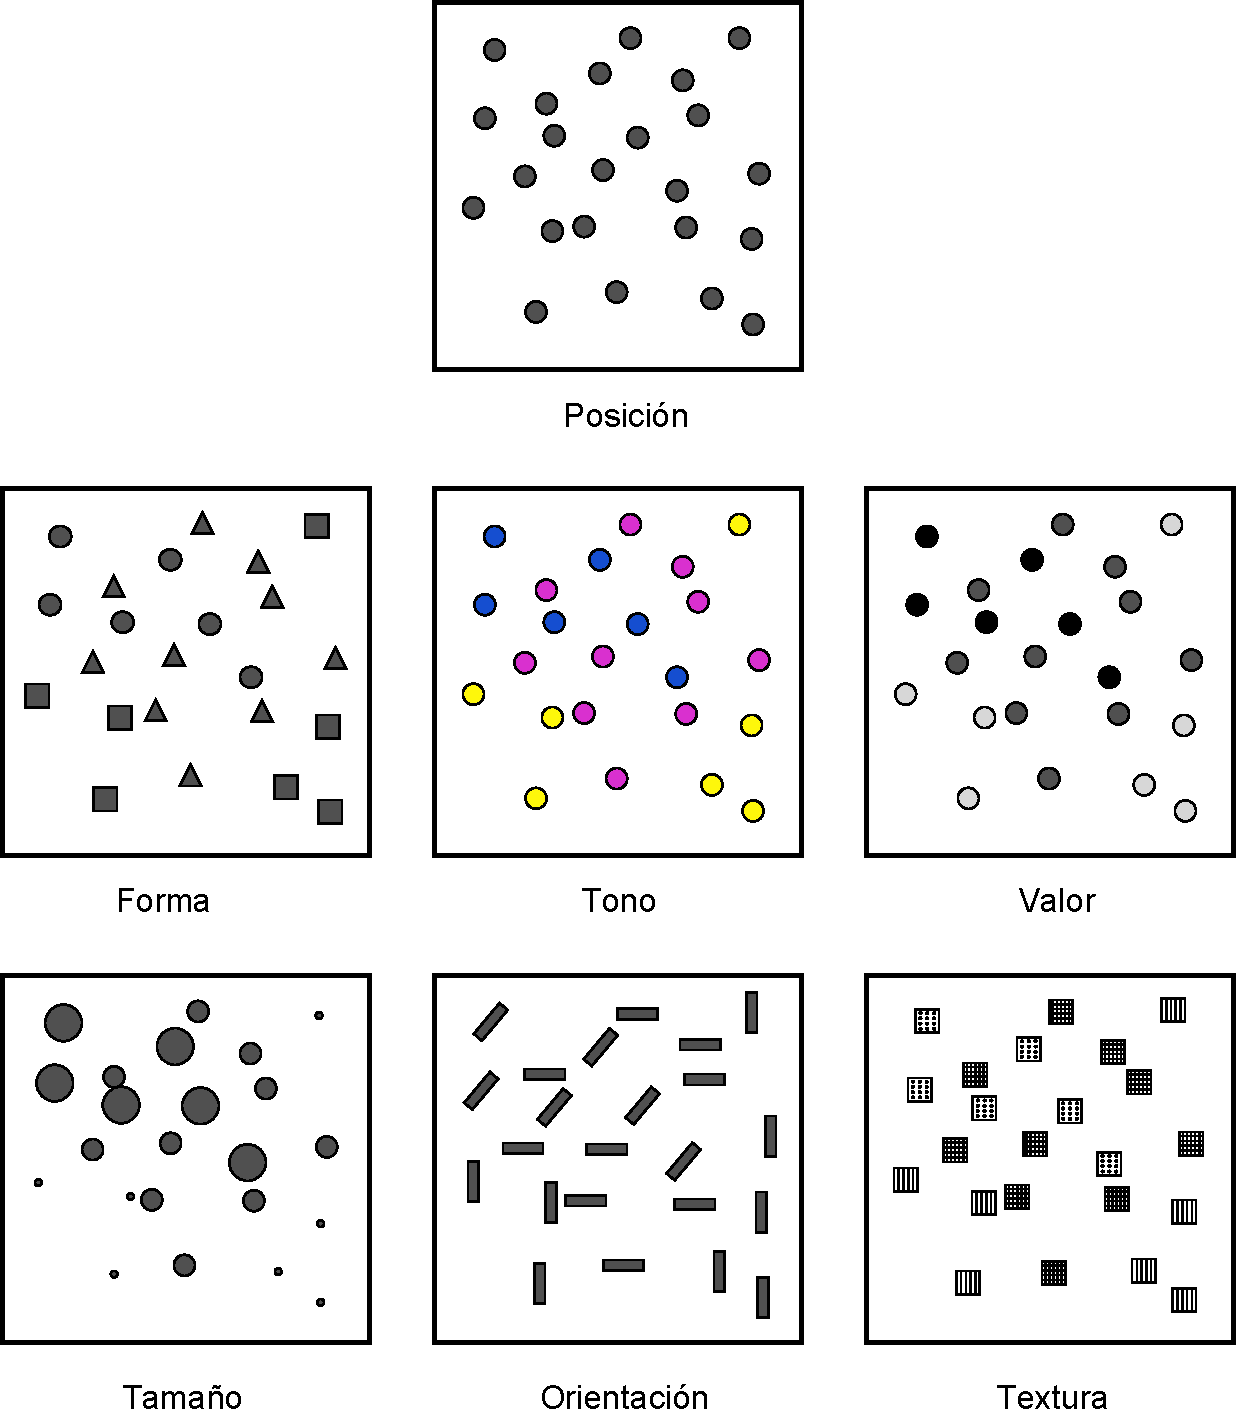
\includegraphics[width=\mycolumnwidth]{Conceptos_basicos/PropiedadesVariablesVisuales.pdf}
\caption{\small Representaci�n de un conjunto de s�mbolos aplicando de forma individual las distintas variables visuales.}
\label{Fig:PropiedadesVariablesVisuales} 
\end{figure}

Comenzando con la propiedad asociativa, vemos que a excepci�n del tama�o y el valor, las dem�s variables visuales no hacen que los elementos presenten una preponderancia en la imagen. No existen una orientaci�n que podamos definir como m�s importante, ni tampoco un color. Lo mismo sucede con la textura, la forma y la posici�n. Podemos emplear una u otra forma, o una u otra textura, y con ello no conseguiremos llamar m�s la atenci�n sobre un elemento en cuesti�n. 

Con el tama�o, sin embargo, resulta claro que mayor tama�o implica un papel destacado dentro de la informaci�n que transmite el mapa. De igual modo, un mayor valor (un color m�s oscuro) da sensaci�n de mayor definici�n, y centra la atenci�n de observador sobre el elemento de un modo muy superior a como lo hace un valor bajo.

Respecto a la propiedad selectiva, diremos que una variable visual la presenta si de un vistazo podemos r�pidamente seleccionar los elementos que pertenecen a un determinado grupo, identificados estos mediante dicha variable visual. El caso m�s claro de propiedad selectiva lo presenta el tono. Podemos r�pidamente quedarnos solo con los elementos amarillos o con los rojos. Aunque no de un modo tan claro, todas las restantes variables presentan igualmente esta propiedad, a excepci�n de la forma. La forma no permite que los elementos se agrupen de modo espont�neo en familias, y su validez en este sentido est� muy ligada a la complejidad de dicha forma.

La propiedad ordenada la presentan aquellas variables que permiten establecer un orden. Tan solo posici�n, textura, tama�o y valor la presentan, mientras que las dem�s carecen de ella. Por ejemplo, en la imagen correspondiente a la variable visual tono no podemos decir cu�les de los elementos situar�amos al principio y cu�les al final de una escala dada definida por esos tonos. Con el valor, sin embargo, s� que podemos, ya que esta escala ir�a de los tonos m�s claros a los m�s oscuros, y visualmente podemos sin dificultad distinguir los distintos niveles y ordenarlos.

Por �ltimo, la propiedad cuantitativa la presentan aquellas variables visuales que permiten estimar proporciones o cantidades de forma visual. Esta propiedad es exclusiva del tama�o y de la posici�n, mientras que las dem�s no la presentan. Podemos visualmente estimar una distancia en comparaci�n con otra y decir que es, por ejemplo, el doble de esta. Tambi�n podemos ver que los c�rculos grandes en la figura correspondiente son aproximadamente el doble que los peque�os. 

El valor, que ya sabemos que presenta la propiedad ordenada, podr�a pensarse que tambi�n presenta la propiedad cuantitativa, pero no sucede as�. Es dif�cil e impreciso afirmar que un color es el doble de oscuro que otro, y lo m�s que podemos hacer es situarlo entre dos valores distintos (de ah� que posea la propiedad ordenada), pero no deducir una cifra que exprese una cantidad o proporci�n. Las restantes variables visuales resulta claro que no poseen esta propiedad.

En el cuadro \ref{Tabla:PropiedadesVariablesVisuales} se muestra un resumen de todo lo anterior.

\begin{table}[!hbt]
\small
\centering  \label{Tabla:PropiedadesVariablesVisuales}
\begin{tabular}{p{3.6cm}ccccccc}  
 & \rotatebox{60}{\textbf{Posici�n}} & \rotatebox{60}{\textbf{Tama�o}} & \rotatebox{60}{\textbf{Forma}} & \rotatebox{60}{\textbf{Valor}} & \rotatebox{60}{\textbf{Tono}} & \rotatebox{60}{\textbf{Textura}} & \rotatebox{60}{\textbf{Orientaci�n}} \\ \midrule   
\textbf{Asociativa}& $\diamondsuit$ & - & $\diamondsuit$ & - & $\diamondsuit$ & $\diamondsuit$ & $\diamondsuit$ \\
\textbf{Selectiva}& $\diamondsuit$ & $\diamondsuit$ & - & $\diamondsuit$ & $\diamondsuit$ & $\diamondsuit$ & $\diamondsuit$ \\
\textbf{Ordenada}&$\diamondsuit$ & $\diamondsuit$ & - & $\diamondsuit$ & - & - & - \\
\textbf{Cuantitativa}& $\diamondsuit$ & $\diamondsuit$ & - & - & - & - & -  \\
\bottomrule \end{tabular}
\caption{\small Cuadro resumen con las propiedades de las variables visuales.}
\end{table}



\section{Uso combinado de las variables visuales}

Para explicar cada una de las variables visuales, hemos visto diversos ejemplos en los que utiliz�bamos cada una de ellas por separado y de forma �nica. Sin embargo, las variables visuales pueden combinarse y, si se hace de la manera correcta, esto reforzar� la capacidad que estas tienen para transmitir una informaci�n dada. La imagen \ref{Fig:CombinacionVariablesVisuales} muestra algunos ejemplos de combinaci�n de variables visuales que nos servir�n para detallar la forma adecuada de usas varias de ellas simult�neamente.

\begin{figure}[!hbt]
\centering
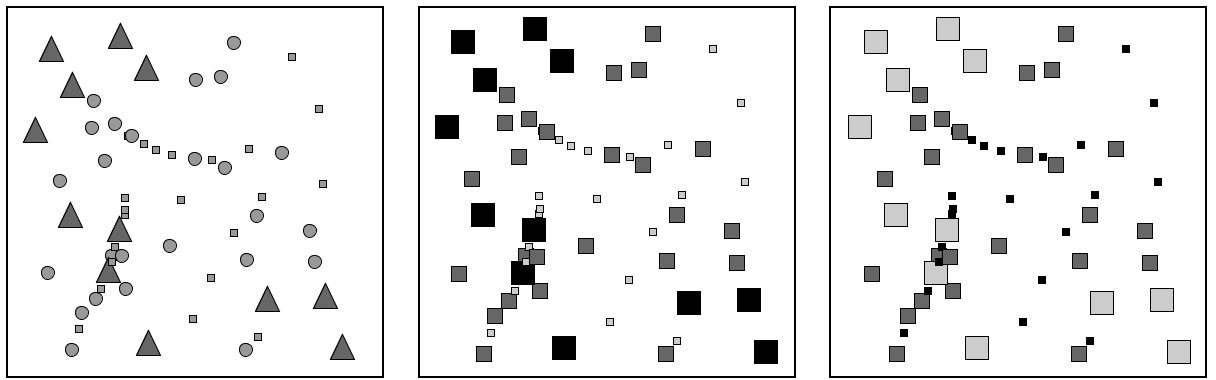
\includegraphics[width=\mycolumnwidth]{Conceptos_basicos/CombinacionVariablesVisuales.png}
\caption{\small Combinaci�n de variables visuales.}
\label{Fig:CombinacionVariablesVisuales} 
\end{figure}

\index{Variables visuales!uso combinado}

El primero de los ejemplos propuestos muestra el uso combinado de las variables tama�o y forma para s�mbolos puntuales. Estos s�mbolos representan la profundidad del suelo medida en determinados emplazamientos, estando relacionado un mayor tama�o del s�mbolo  con una profundidad mayor. Asimismo, se ha asociado un s�mbolo triangular a los valores m�s bajos, un s�mbolo circular a los intermedios y uno cuadrado a los m�s altos. Aunque se emplean dos variables visuales distintas, el resultado no es, sin embargo, mejor que en caso de emplear uno solo de ellos (en este caso, deber�a emplearse el tama�o, ya que la forma no presenta la propiedad cuantitativa necesaria para representar cantidades). Lejos de producirse una sinergia entre el efecto de ambas variables, el resultado es similar al uso exclusivo del tama�o en cuanto a su capacidad de transmitir la informaci�n, o incluso peor, ya que la forma puede dificultar la estimaci�n visual del tama�o, al ser m�s complicado comparar la dimensi�n de objetos de distinta forma.

Pese a que no es clara la ventaja de aplicar conjuntamente las variables forma y tama�o, esta puede emplearse para representar cantidades, por lo que podemos decir que mantiene la propiedad cuantitativa que posee el tama�o. En general, al combinar dos variables visuales el resultado presentara las propiedades de aquella que tenga un mayor nivel organizativo. Puesto que la propiedad cuantitativa representa el nivel organizativo superior, en este caso se mantiene en la combinaci�n.

A�n as�, hay mejores formas de combinar las variables visuales para que esta combinaci�n enfatice en mayor grado la informaci�n que se pretende transmitir, como por ejemplo la mostrada en el segundo ejemplo. Este ejemplo combina el tama�o y el valor, variables ambas que no poseen la propiedad asociativa. Es decir, poseen su complementaria, que podr�amos denominar \emph{disociativa}, y que, recordemos, es la propiedad que, al aplicarse sobre un s�mbolo, hace que este gane importancia visual. El resultado presenta un car�cter todav�a m�s disociativo, en cuanto que los s�mbolos que representan una cantidad elevada, al ser no solo grandes, sino estar pintados en color oscuro, llaman a�n m�s nuestra atenci�n que si emple�ramos una �nica de las variables visuales utilizadas.

Como regla en este sentido, podemos decir que, cuando se combinan variables visuales que poseen una determinada propiedad, en el resultado esta propiedad queda reforzada con respecto a las variables individuales.

El tercer ejemplo nos muestra que combinar variables visuales con una misma propiedad no garantiza necesariamente que se vaya a producir una sinergia entre ellas, sino que, por el contrario, pueden anularse. Las variables empleadas en este caso son las mismas, valor y tama�o, pero se ha asociado el color claro a los valores mayores y el oscuro a los menores, de tal modo que los s�mbolos de mayor tama�o son m�s claros que los peque�os. Esto aten�a el efecto disociativo del tama�o, de forma que la representaci�n es m�s dif�cil de interpretar y su informaci�n no se transmite de modo tan inmediato y directo.

En resumen, podemos sintetizar lo anterior diciendo que, a la hora de combinar variables visuales, deben tenerse en cuenta las propiedades de estas del mismo modo que cuando se emplean de forma individual. Las propiedades a reforzar ser�n aquellas que convengan m�s al tipo de informaci�n representado, y deben presentarlas todas las variables a combinar para que el efecto conjunto sea m�s acusado.


\section{La percepci�n visual}

La percepci�n engloba toda la serie de procesos que convierten un fen�meno f�sico en una informaci�n acerca de nuestro entorno, a trav�s de la estimulaci�n de unos �rganos perceptivos. La percepci�n tiene una fase f�sica, una fisiol�gica (la estimulaci�n en s�) y una psicol�gica (la interpretaci�n del est�mulo). En el caso de la percepci�n visual, este fen�meno f�sico es de tipo energ�tico (la luz), y los �rganos correspondientes son los ojos. \index{Percepci�n visual}

El estudio de la percepci�n es un fen�meno complejo que no entraremos a detallar, pero en el que resulta de inter�s profundizar para conocer algo m�s acerca de c�mo la informaci�n que plasmamos en un mapa (que es un elemento visual) acaba convertida en una informaci�n en la mente del observador de ese mapa. Entender este proceso, al menos someramente, nos permitir� mejorar la eficacia de la percepci�n, de forma que tengamos una mayor garant�a de que la informaci�n que transmitimos sea recibida e interpretada correctamente.

Dos son los aspectos que detallaremos en esta secci�n: las constancias perceptivas y las ayudas a la percepci�n. En otras palabras, hasta qu� punto podemos modificar los elementos visuales o su entorno sin que dejen de transmitir su informaci�n y sean confundidos sus caracter�sticas, y c�mo podemos facilitar que se perciban exactamente como pretendemos.

\subsection{Las constancias y contrastes perceptivos}

Entendemos por constancias perceptivas a las propiedades de los objetos cuya percepci�n no var�a aunque se produzcan modificaciones. Podemos ver algunos ejemplos para algunas de las variables visuales que conocemos.

\index{Constancia perceptiva}\index{Contraste perceptivo}

Dado un objeto redondo tal como una rueda, si lo miramos en una direcci�n perpendicular aparecer� efectivamente como una forma circular perfecta. Sin embargo, si la miramos desde otro �ngulo, veremos una forma el�ptica, pero ello no nos lleva a pensar que la rueda en s� no sea ya redonda. Nuestra percepci�n de esa rueda es la misma, y podemos apreciar de igual modo su tama�o o su forma. Alterar el �ngulo de visi�n no altera el objeto y la percepci�n que tenemos de �l.

Del mismo modo, un elemento pintado de un color claro se identifica como tal aunque la luz sea tenue, y un elemento oscuro lo seguimos percibiendo como oscuro aunque estemos en unas condiciones de iluminaci�n fuerte. Nuestro cerebro es capaz de interpretar simult�neamente el objeto y el contexto, y de este modo extraer las caracter�sticas de ese objeto, que no var�an.

Estos dos ejemplos muestran la constancia perceptiva de la forma y el valor, y podemos buscar otros similares para otras variables visuales.

No todas las variables visuales tienen una constancia perceptiva como la anterior. Todos conocemos m�ltiples ejemplos de ilusiones �pticas en las que algo no parece lo que realmente es, y esa percepci�n err�nea viene normalmente motivada por las condiciones en las que percibimos el objeto, por ejemplo debido al entorno particular en el que este se encuentra junto a otros objetos. La figura \ref{Fig:Zollner} muestra un ejemplo cl�sico de ilusi�n �ptica, conocida como \emph{ilusi�n de Zollner}. Las lineas largas diagonales son paralelas, pero no aparentan serlo, debido al efecto causado por las l�neas m�s cortas. En este caso, no existe una constancia perceptiva de la variable visual orientaci�n.

\index{Ilusi�n de Zollner}

Cuando la percepci�n de un elemento cambia aunque el estimulo no lo haga, en lugar de una constancia perceptiva hablamos de un \emph{contraste perceptivo}. Los contrastes perceptivos son importantes, ya que pueden inducir una interpretaci�n err�nea de la informaci�n que pretendemos transmitir, al producirse una percepci�n equivocada.


\begin{figure}[!hbt]
\centering
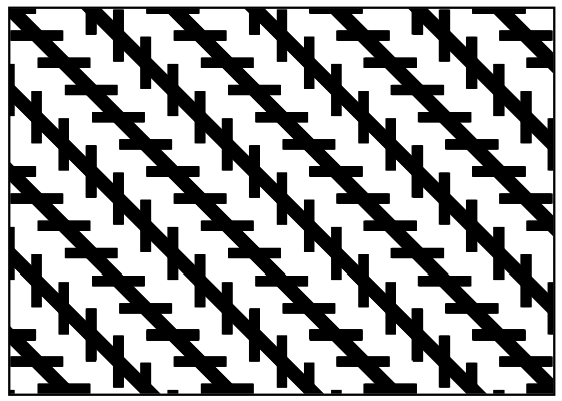
\includegraphics[width=.4\mycolumnwidth]{Conceptos_basicos/Zollner_illusion.png}
\caption{\small Ilusi�n de Zollner que demuestra el contraste perceptivo de la orientaci�n.}
\label{Fig:Zollner} 
\end{figure}

Las siguientes son algunas de las ideas m�s importantes a tener en cuenta a este respecto a la hora de crear un mapa:

\begin{itemize}
	\item El tama�o es la variable visual que m�s afectada se ve, y el tama�o aparente de un objeto puede variar notablemente si se encuentra rodeado de otros de un tama�o distinto. La figura \ref{Fig:ContrasteTamano} muestra un ejemplo de esto. A la hora de emplear simbolog�a de elementos puntuales en un mapa (por ejemplo, en un mapa de s�mbolos graduados, como veremos en el apartado \ref{MapasSimbolosGraduados}), esto debe tenerse en cuenta, ya que pueden presentarse situaciones como la de la figura.	
	\item El valor se ve igualmente alterado al situar alrededor elementos de distinto valor. Si el n�mero de distintos valores es peque�o, es m�s dif�cil que aparezca este contraste perceptivo. A medida que se aumenta el n�mero de estos, es m�s probable que aparezca en mayor o menor medida.
	\item El tono se ve alterado por la presencia de otros tonos distintos. En un mapa, veremos este efecto al enfrentar el color de un elemento sobre el color del fondo. Por ejemplo, si una l�nea que representa a una carretera y cruza una serie de pol�gonos de distinto tono, puede parecer que el tono de la l�nea varia aunque en realidad sea constante.
	\item Tonos complementarios puestos juntos pueden crear sensaci�n de vibraci�n en la frontera que los separa.
\end{itemize}

\begin{figure}[!hbt]
\centering
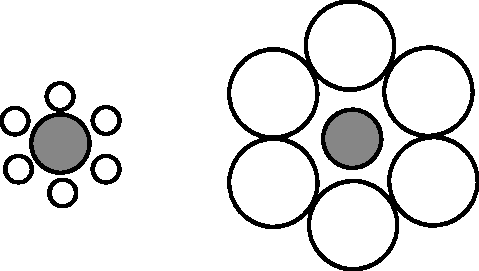
\includegraphics[width=.5\mycolumnwidth]{Conceptos_basicos/ContrasteTamano.pdf}
\caption{\small Contraste perceptivo del tama�o. Ambos circulos grises tienen el mismo tama�o, pero el de la izquierda aparenta ser mayor.}
\label{Fig:ContrasteTamano} 
\end{figure}

\subsection{Ayudas a la percepci�n}
\label{AyudasPercepcion}

Con lo que hemos visto anteriormente, queda claro que podemos alterar la forma en que se perciben las variables visuales que caracterizan a un elemento visual. Podemos usar este hecho para nuestro beneficio, de tal modo que el dise�o de un mapa incorpore elementos que hagan m�s patente la informaci�n que este contiene, facilitando la correcta percepci�n del mapa en su conjunto.

Un factor clave en este sentido es la adecuado separaci�n entre el fondo y la figura. Aquello que queremos que resulte visible con car�cter principal (en el caso de un mapa, sus distintos elementos) debe separarse de aquello que constituye el fondo de la imagen, y debe atraer la atenci�n del observador de manera prioritaria. En caso de no ser as�, puede resultar dif�cil <<descubrir>> la informaci�n que el mapa transmite, al quedar esta al mismo nivel que la de otros elementos de menor importancia. El ejemplo cl�sico de la figura \ref{Fig:CupOrFaces} ilustra este hecho. Puesto que no existe una diferenciaci�n clara entre el fondo y la figura, no es obvio saber si la imagen pretende representar una copa o dos caras.

\begin{figure}[!hbt]
\centering

\includegraphics[width=.25\mycolumnwidth]{Conceptos_basicos/Cup_or_faces_paradox.pdf}
\caption{\small Sin un adecuado contraste entre fondo y figura la imagen presenta ambig�edad.}
\label{Fig:CupOrFaces} 
\end{figure}

En un mapa, y como veremos en el pr�ximo cap�tulo, encontramos dos tipos de cartograf�a: una con car�cter de base que define un contexto geogr�fico, y una tem�tica que constituye la informaci�n principal que se transmite con el mapa. Puesto que esta segunda es la fundamental y de mayor importancia, y la primera se incluye tan solo como apoyo de esta, es importante asegurarse de que esa cartograf�a base no interfiere y se mantiene en un segundo plano, constituy�ndose como fondo y dejando que sea la informaci�n tem�tica la que act�e como figura. Para ello podemos emplear las distintas variables visuales aplicadas a la cartograf�a base, de modo que su importancia relativa no sea mayor que la de los elementos principales de la parte tem�tica.

Otro aspecto a considerar es la adecuada jerarquizaci�n entre los elementos del mapa. La divisi�n entre fondo y figura ya constituye en s� una jerarquizaci�n, pero no es suficiente si conviven varios tipos de elementos en el mapa. Dentro de la parte tem�tica es necesario estructurar estos visualmente para que quede clara su importancia y se vea sin dificultad que existe una divisi�n entre ellos.\index{Jerarquizaci�n}\index{Fondo--figura}

Esta jerarqu�a debe aportar una <<profundidad>> a la informaci�n, de forma que existan niveles en esta y se perciba que algunos elementos est�n por encima de otros. Como veremos en el cap�tulo \ref{Visualizacion_SIG}, la forma de ordenar las distintas capas en un SIG ya establece un orden, aunque este no es en s� suficiente, y deben utilizarse las variables visuales para enfatizar o no unas o otras capas y la informaci�n que contienen.

Algunas t�cnicas b�sicas para esto son las que permiten que exista alg�n factor diferencial en la informaci�n m�s relevante. Si las propiedades de los elementos destacados difieren notablemente de las del fondo, esto centra la atenci�n sobre ellas y garantiza que no se confundan con este. Emplear unas caracter�sticas m�s homog�neas para el fondo permite que la diferenciaci�n de la figura sea m�s patente. En otras palabras, el contraste, aplicado este a todas las variables visuales, es una de las claves para lograr una adecuada transmisi�n de la informaci�n al emplear una representaci�n visual.

El contraste se aplica no solo a las variable visuales, sino en general a las caracter�sticas de la representaci�n. Por ejemplo, el nivel de detalle es una propiedad susceptible de ser utilizada para enfatizar algo. As�, y en el caso particular del documento cartogr�fico, el lector de un mapa espera que el detalle sea mayor en la cartograf�a tem�tica que en la de base, ya que esta �ltima es simplemente un elemento complementario de ayuda. Un mayor detalle sobre ciertos elementos llamar� m�s la atenci�n en contrate con un fondo menos detallado, y esto puede utilizarse para enfocar la atenci�n sobre lo m�s relevante. Ofrecer menos detalle en la cartograf�a de base no es un inconveniente si esto ayuda a un mejor entendimiento de los elementos principales del mapa.

Como ejemplo de lo anterior, la figura \ref{Fig:JerarquiaMapa} muestra un ejemplo de como una correcta jerarquizaci�n es fundamental para crear mapas de calidad.

\begin{figure}[!hbt]
\centering
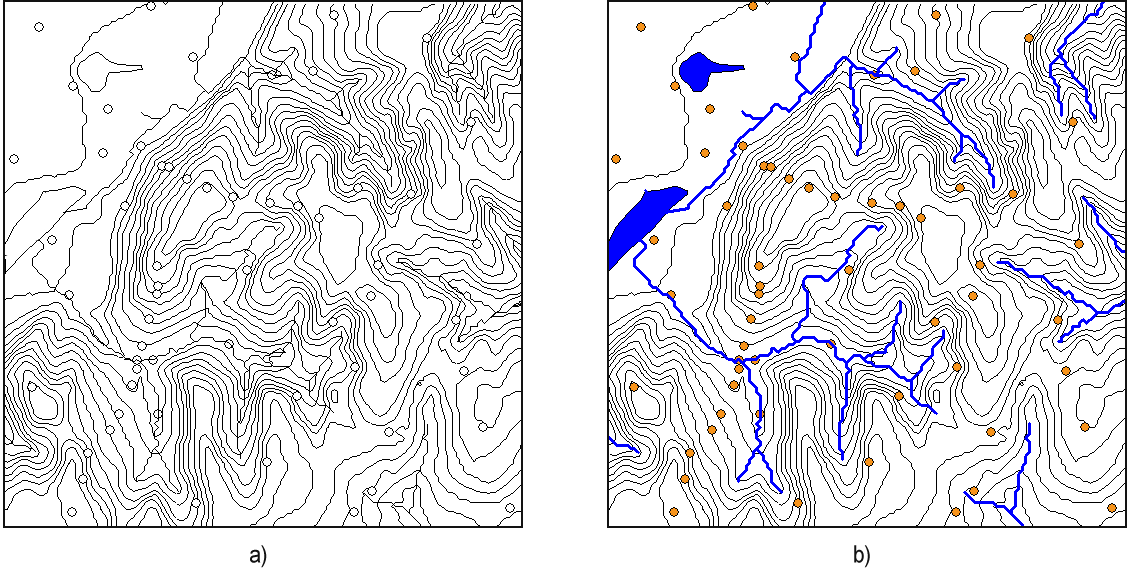
\includegraphics[width=\mycolumnwidth]{Conceptos_basicos/JerarquiaMapa.png}
\caption{\small Mapa con jerarqu�a incorrecta (a) y mapa adecuadamente jerarquizado (b).}
\label{Fig:JerarquiaMapa} 
\end{figure}

Por �ltimo, un aspecto clave para la claridad de un mapa es el relativo al poder separador. Este define la capacidad de un individuo para distinguir objetos muy peque�os y separar objetos cercanos. Adem�s de depender del propio individuo, est� condicionado por una serie de factores. 

Se admite en l�neas generales que el l�mite de separaci�n entre dos objetos para el ojo humano es de 0,2mm. Si existe una distancia menor entre ellos, en condiciones normales no ser� posible distinguir uno de otro. \index{Limite@L�mite de separaci�n}

Existe tambi�n un l�mite para poder reconocer objetos aislados, aunque este depende del tipo de objeto. Los siguientes son algunos de los aplicados usualmente:

\begin{itemize}
	\item 0,2mm de diametro para el caso de un punto.
	\item 0,5mm de grosor para el caso de una l�nea negra.
	\item 0,4mm de lado para el caso de un cuadrado negro.
	\item 0,6mm de lado para un cuadrado sin relleno.
\end{itemize}

Existe asimismo un umbral de diferenciaci�n, que define el tama�o m�nimo de dos objetos para que puedan ser percibidos como distintos. Este umbral tambi�n depende de las caracteristicas de los objetos, como por ejemplo la forma (si las formas son muy distintas ser� m�s f�cil distinguirlos que si son muy similares). 

El poder separador no depende �nicamente de variables de tipo espacial, sino que tambi�n est� en relaci�n con otras variables visuales. Por ejemplo, una l�nea negra sobre fondo blanco puede distinguirse aunque sea fina, pero en caso de ser amarilla sobre ese mismo fondo, ser� necesario un grosor mayor.

Como parece l�gico, estos conceptos deben usarse para no incorporar a un mapa elementos que est�n m�s all� del umbral de separaci�n del lector del mapa, ya que en este caso no podr� extraer la informaci�n que se ha incorporado en este al crearlo.




\pagestyle{empty} 
\end{mainmatter}

\cleardoublepage

\end{document}


